% PhD thesis
\documentclass[12pt,twoside,openright]{report}
\usepackage{etex}
\usepackage[all]{xy}
\usepackage{pb-diagram}
\usepackage{amsfonts, amssymb, amsmath}
\usepackage{tikz}
\usepackage{bussproofs}
\usepackage{epsfig}
\usepackage{hyperref}
\usepackage{latexsym,url}
\usepackage{txfonts}
\usepackage{undertilde}
\usepackage[pdf]{pstricks}
\usepackage{pstricks-add, pst-grad, pst-plot}
\usepackage[tiling]{pst-fill}
\usepackage{pstcol}
\PassOptionsToPackage{hyphens}{url}\usepackage{hyperref}
\usetikzlibrary{matrix,arrows}
\usetikzlibrary{backgrounds}
\usetikzlibrary{decorations.pathmorphing}
\usetikzlibrary{decorations.pathreplacing}
\usetikzlibrary{decorations.shapes}
\usetikzlibrary{decorations.markings}
\usetikzlibrary{calc}
% PsTricks defaults
\psset{linewidth=0.3pt,dimen=middle}
\psset{xunit=.70cm,yunit=0.70cm}

\tikzset{l/.style={font=\fontsize{8}{8}\selectfont}}
\tikzset{m/.style={font=\fontsize{6}{6}\selectfont}}
\tikzset{
electron/.style={postaction=decorate, decoration={markings, mark=at position 0.55 with {\arrow{triangle 45}}}}, photon/.style={decorate, decoration={coil, aspect=0}}
}
\definecolor{salmon}{rgb}{1,0.47,0.425}
%\definecolor{purple}{rgb}{0.5,0,0.5}


\textwidth = 6.5 in
\textheight = 9 in
\oddsidemargin = 0.0 in
\evensidemargin = 0.0 in
\topmargin = 0.0 in
\headheight = 0.0 in
\headsep = 0.0 in
\parskip = 0.1in
\parindent = 0.0in

% theorem environments
\newtheorem{thm}{Theorem}
\newtheorem{definition}[thm]{Definition}
\newtheorem{defn}{Definition}
\newtheorem{lemma}{Lemma}

%famous sets
\newcommand{\RR}{\mathbb{R}}
\newcommand{\QQ}{\mathbb{Q}}
\newcommand{\NN}{\mathbb{N}}
\newcommand{\CC}{\mathbb{C}}
\newcommand{\ZZ}{\mathbb{Z}}

%famous categories
\newcommand{\Cob}{\mathrm{Cob}}
\newcommand{\Hilb}{\mathrm{Hilb}}
\newcommand{\Set}{\mathrm{Set}}
\newcommand{\Fin}{\mathrm{Fin}}
\newcommand{\Cat}{{\rm Cat}}
\newcommand{\Tang}{{\rm Tang}}
\newcommand{\Lie}{{\rm Lie}}
\newcommand{\Grp}{{\rm Grp}}
\newcommand{\CommRing}{{\rm CommRing}}
\newcommand{\Diff}{{\rm Diff}}
\newcommand{\Rep}{{\rm Rep}}
\newcommand{\Vect}{{\rm Vect}}
\newcommand{\Braid}{{\rm Braid}}
\newcommand{\Rel}{{\rm Rel}}
\newcommand{\Super}{{\rm Super}}
\newcommand{\Th}{\mathrm{Th}}

%arrows
\newcommand{\maps}{\colon}
\newcommand{\iso}{\cong}
\newcommand{\isoto}{\stackrel{\sim}{\to}}
\newcommand{\To}{\Rightarrow}

%homs
\newcommand{\lHom}{\vdash}
\newcommand{\lhom}{\multimap}
\newcommand{\rhom}{\leftspoon}
\renewcommand{\hom}{{\rm hom}}
\newcommand{\HOM}[2]{{#1 \lhom #2}}

%products
\newcommand{\tensor}{\otimes}
\newcommand{\x}{\times}
\newcommand{\OTIMES}{{\boldmath$\otimes$ \,}}
\newcommand{\TENSOR}{{\boldmath$\hat{\otimes}$ \,}}
\newcommand{\CIRC}{{\boldmath$\circ$ \,}}
\newcommand{\LAMBDA}{{\boldmath$\lambda$ \,}}
\newcommand{\ab}[1]{\langle #1 \rangle} % "angle brackets"

%morphisms, rules, constants
\newcommand{\id}{{\rm i}}
\newcommand{\Id}{{\rm id}}
\newcommand{\ev}{{\rm ev}}
\newcommand{\coev}{{\rm coev}}
\newcommand{\eval}{{\rm eval}}
\newcommand{\app}{{\rm app}}
\newcommand{\assoc}{{\rm assoc}}
\newcommand{\unassoc}{{\rm unassoc}}
\newcommand{\braid}{{\rm braid}}
\newcommand{\Left}{{\rm left}}
\newcommand{\Right}{{\rm right}}
\newcommand{\unright}{{\rm unright}}
\newcommand{\unleft}{{\rm unleft}}
\newcommand{\Tensor}{{\rm tensor}}
\newcommand{\swap}{{\rm swap}}
\newcommand{\term}{{\rm term}}
\newcommand{\cp}{{\rm cp}}
\newcommand{\vp}{{\rm vp}}
\newcommand{\cut}{{\circ}}
\newcommand{\op}{{\rm op}}   
\newcommand{\name}[1]{\ulcorner \! #1 \! \urcorner}
\newcommand{\inv}{${}^{-1}$}

%data types and programs
\newcommand{\plus}{{\rm plus}}
\newcommand{\Times}{{\rm times}}
\newcommand{\double}{{\rm double}}
\newcommand{\increment}{{\rm increment}}
\newcommand{\Day}{{\rm day}}
\newcommand{\Tuesday}{{\rm Tuesday}}
\newcommand{\integer}{{\rm integer}}
\newcommand{\duplicate}{{\rm duplicate}}
\newcommand{\curry}{{\rm curry}}
\newcommand{\uncurry}{{\rm uncurry}}
\newcommand{\compose}{{\rm compose}}

%chemical elements
\renewcommand{\H}{H}
\renewcommand{\O}{O}

%formatting commands
\newcommand{\apos}{{\boldmath${}'$}}
\newcommand{\cent}[1]{\begin{center} #1 \end{center}}
\newcommand{\al}[1]{\begin{align} #1 \end{align}}
\renewcommand{\thefootnote}{\fnsymbol{footnote}}
\newcommand {\tuple}[1]{\langle #1 \rangle}
\newcommand{\di}[1]{\[\begin{diagram}#1\end{diagram}\]}
\newcommand{\xeq}[1]{{\displaystyle \mathop{=}_{#1}}}
\renewcommand{\text}{\mbox}
\newcommand{\QUOTE}[1]{\begin{quote} {\tt #1 } \end{quote}}
\newcommand{\mbold}[1]{\mbox{\bf #1}}
\newcommand{\too}{\Rightarrow}
\newcommand{\isotoo}{\; \tilde{\Rightarrow} \;}


\newcommand{\et}{\hspace{-0.08in}{\bf .}\hspace{0.1in}}   
\newcommand{\Hom}{\mbox{Hom}}
\newcommand{\FinSet}{\mbox{FinSet}}
\newcommand{\Aut}{\mbox{Aut}}
\newcommand{\Span}{\mbox{Span}}
\newcommand{\Ob}{\mbox{Ob}}
\newcommand{\Mor}{\mbox{Mor}}
\newcommand{\Cocont}{\mbox{Cocont}}
\newcommand{\MatN}{\ensuremath{\mbox{Mat(\NN)}}}
\newcommand{\nCob}{n\mbox{Cob}}
\newcommand{\Tr}{\mbox{Tr}}

\newcommand{\comod}{\textnormal{Comod}  }
\newcommand{\rev}{\textnormal{rev} }
\newcommand{\comodf}{\textnormal{Comod}_f  }
\newcommand{\coalg}{ \textnormal{Coalg}  }
\newcommand{\comonadic}{ \textnormal{Comonadic}  }
\newcommand{\cocent}{ \textnormal{Cocent}  }
\renewcommand{\mod}{ {\textnormal{Mod}}  }
\newcommand{\vact}{ \V  {\textnormal{-Act}}  }
\newcommand{\catvv}{ \textnormal{Cat} / \negthinspace / \V  }
\newcommand{\cotr} { \textnormal{Cotract}  }
\newcommand{\vactv}{ {\mathcal{V}} {\textnormal{-Act}}  / \V  }
\newcommand{\catvf}{  \cat  / {\V_f}  }
\newcommand{\catvectf}{  \cat  / {\vectf}  }
\newcommand{\catv}{  \cat  / \V  }
\newcommand{\vactvv}{ \vact  / \negthinspace / \V }
\newcommand{\Ach}{\ensuremath {A_{\textnormal{ch}}}  }
\newcommand{\ench}{\ensuremath {\textnormal{End}}^{\vee}  }
\newcommand{\coend}{\ensuremath {\textnormal{coend}} }
\newcommand{\V}{ {\mathcal{V}}  }
\newcommand{\W}{ {\mathcal{W}}  }
\newcommand{\A}{ {\mathcal{A}}  }
%\newcommand{\B}{ {\mathcal{B}}  }
\newcommand{\C}{ {\mathcal{K}}  }
\newcommand{\D}{ {\mathcal{D}}  }
\newcommand{\K}{ {\mathcal{K}}  }
\renewcommand{\L}{ {\mathcal{L}}  }
\newcommand{\M}{ {\mathcal{M}}  }
\newcommand{\U}{ {\mathcal{U}}  }
\newcommand{\X}{ {\mathcal{X}}  }
\newcommand{\comoda}{ S }
\newcommand{\comodb}{  T }
\newcommand{\cat}{ {\textnormal{Cat}}  }
\newcommand{\sq}{ {\textnormal{Sq}}  }
\newcommand{\comp}{ \C  }
%\newcommand{\gray}{ {\textnormal{Gray}}  }
\newcommand{\obj}{ {\textnormal {obj}}  }
\newcommand{\vect}{ {\textnormal{Vect}}  }
\newcommand{\vectf}{ {\textnormal{Vect}}_f  }
\newcommand{\E}{ {\textnormal{E}}  }
\newcommand{\comon}{ {\textnormal{Comon}}  }
\newcommand{\mon}{ {\textnormal{Mon}}  }
\newcommand{\vopcat}{ \V^{\textnormal{op}} {\textnormal{-Cat}}  }
\newcommand{\vopcatop}{ \vopcat^{\textnormal{op}}  }
\newcommand{\vcat}{ \V {\textnormal{-Cat}}  }
\newcommand{\set}{ {\textnormal{Set}}  }
\newcommand{\disc}{ {\mathbb{D}}  }
\newcommand{\Vop}{ {\V^{\textnormal{op}}}  }
\newcommand{\desc}{ {\textnormal{Desc}}  }
\newcommand{\lbr}{ [ \negthinspace [  }
\newcommand{\rbr}{ ] \negthinspace ]  }
\newcommand{\psmon}{ \textnormal{PsMon}   }
\newcommand{\brpsmon}{ \textnormal{BrPsMon}  }
\newcommand{\sympsmon}{ \textnormal{SymPsMon}  }
\newcommand{\balpsmon}{ \textnormal{BalPsMon}  }
\newcommand{\cone}{  \textnormal{Cone}  }
\newcommand{\wmonhom}{ \textnormal{WMon}  }
\newcommand{\brwmonhom}{ \textnormal{BrWMon}  }
\newcommand{\syllwmonhom}{ \textnormal{SyllWMon}  }
\newcommand{\balwmonhom}{ \textnormal{BalWMon}  }
\newcommand{\symwmonhom}{ \textnormal{SymWMon}  }
%\newcommand{\assoc}{{\sf{a}}}
%\newcommand{\leftunit}{{\sf{l}}}
%\newcommand{\rightunit}{{\sf{r}}}
%\newcommand{\mqn}{ M_q(n)}
\newcommand{\acirc}{ {\stackrel{\mbox{\circle{2}}}{a}} }
\newcommand{\lcirc}{ {\stackrel{\mbox{\circle{2}}}{l}} }
\newcommand{\rcirc}{ {\stackrel{\mbox{\circle{2}}}{r}} }

\newcommand{\ctr}[1]{\begin{center} #1 \end{center}}
\newcommand{\oo}{\infty}
\newcommand{\alx}[1]{\begin{align*} #1 \end{align*}}
\renewcommand{\L}{\mathfrak{L}}
\newcommand{\N}{\mathbb{N}}
\newcommand{\R}{\mathbb{R}}
\newcommand{\prf}{\noindent {\em Proof.}  }
\newcommand{\QED}{\hfill $\square$}
\newcommand{\dom}{\mbox{\rm dom}}
\newcommand{\bin}{\mbox{bin}}
\newcommand{\Iota}{\mbox{{\tiny Iota}}}
\newcommand{\floor}[1]{\lfloor #1 \rfloor}
\renewcommand{\thefootnote}{\fnsymbol{footnote}}
\newcommand{\fdom}{\mbox{\rm \footnotesize{dom}}}
\newcommand{\fbin}{\mbox{\rm \footnotesize{bin}}}
\newcommand{\COM}[2]{{#1 \choose #2}}
\newcommand{\Prob}{{\rm Prob}}
\newcommand{\Halt}{{\rm Halt}}
\newcommand{\ttime}{{\rm time}}
\newtheorem{fact}[thm]{Fact}
\newtheorem{lem}[thm]{Lemma}
\newtheorem{cor}[thm]{Corollary}
\newtheorem{example}[thm]{Example}
\newtheorem{sch}[thm]{Scholium}
\newcommand{\myproof}{\noindent {\em Proof.}  }
\newcommand{\Space}{\mbox{Space}}


%pictures of cobordisms

\newcommand{\multc}{
  \begin{scope}[left color=gray, right color=white]
    \shadedraw (1.5,2.5) 
      .. controls (1.5,1.1) and (.4,1.6) .. (.5,0) 
      .. controls (.4,-.25) and (-.4,-.25) .. (-.5,0)
      .. controls (-.4,1.6) and (-1.5,1.1) .. (-1.5,2.5)
      -- (-.5,2.5)
      .. controls (-.6,1.5)and (0.6,1.5) .. (.5,2.5)
      -- (1.5,2.5);
    \shadedraw (-1,2.5) ellipse (.5 and .2);
    \shadedraw (1,2.5) ellipse (.5 and .2);
  \end{scope}
  \draw[dashed] (0.5,0) arc (0:180:.5 and .2);
}

\newcommand{\comultc}{
  \begin{scope}[left color=gray, right color=white]
    \shadedraw (1.5,0) 
      .. controls (1.5,1.4) and (.4,.9) .. (.5,2.5)
      -- (-0.5,2.5)
      .. controls (-.4,.9) and (-1.5,1.4) .. (-1.5,0)
      .. controls (-1.4,-.25) and (-.6,-.25) .. (-.5,0)
      .. controls (-.6,1) and (0.6,1) .. (.5,0)
      .. controls (.6,-.25) and (1.4,-.25) .. (1.5,0);
    \shadedraw (0,2.5) ellipse (.5 and .2);
  \end{scope}
  \draw[dashed] (1.5,0) arc (0:180:.5 and .2);
  \draw[dashed] (-.5,0) arc (0:180:.5 and .2);
}

\newcommand{\identc}{
  \begin{scope}[left color=gray, right color=white]
    \shadedraw (.5,0) -- (.5,2.5) -- (-.5,2.5) -- (-.5,0) 
      .. controls (-.4,-.25) and (.4,-.25) .. (.5,0);
    \shadedraw (0,2.5) ellipse (.5 and .2);
  \end{scope}
  \draw[dashed] (0.5,0) arc (0:180:.5 and 0.2);
}

\newcommand{\medidentc}{
  \begin{scope}[left color=gray, right color=white]
    \shadedraw (-.5,2) -- (-.5,0)
      .. controls (-.4,-.25) and (.4,-.25) .. (.5,0)
      -- (.5,2) -- (-.5, 2);
    \shadedraw (0,2) ellipse (.5 and .2);
  \end{scope}
  \draw[dashed] (0.5,0) arc (0:180:.5 and 0.2);
}

\newcommand{\smallidentc}{
  \begin{scope}[left color=gray, right color=white]
    \shadedraw (-.5,1) -- (-.5,0)
      .. controls (-.4,-.25) and (.4,-.25) .. (.5,0)
      -- (.5,1) -- (-.5, 1);
    \shadedraw (0,1) ellipse (.5 and .2);
  \end{scope}
  \draw[dashed] (0.5,0) arc (0:180:.5 and 0.2);
}

\newcommand{\birthc}{
  \begin{scope}[left color=gray, right color=white]
    \shadedraw (-.5,0)
      .. controls (-.5,.9) and (0.5,.9) .. (.5,0)
      .. controls (.4,-.25) and (-.4,-.25) .. (-.5,0);
  \end{scope}
  \draw[dashed] (0.5,0) arc (0:180:.5 and 0.2);
}

\newcommand{\deathc}{
  \begin{scope}[left color=gray, right color=white]
    \shadedraw (-.5,1)
      .. controls (-.5,.1) and (0.5,.1) .. (.5,1)
      -- (-.5,1);
    \shadedraw (0,1) ellipse (.5 and .2);
  \end{scope}
}

\newcommand{\ucrossc}{
  \begin{scope}[left color=gray, right color=white]
    \shadedraw (.5,0) -- (-1.5,2.5) -- (-.5,2.5) -- (1.5,0)
       .. controls (1.4,-.25) and (.6,-.25) .. (.5,0);
    \shadedraw (-.5,0) -- (1.5,2.5) -- (.5,2.5) -- (-1.5,0)
       .. controls (-1.4,-.25) and (-.6,-.25) .. (-.5,0);
    \shadedraw (-1,2.5) ellipse (.5 and .2);
    \shadedraw (1,2.5) ellipse (.5 and .2);
  \end{scope}
  \draw[dashed] (-1.5,2.5) -- (.5,0);
  \draw[dashed] (-.5,2.5) -- (1.5,0);
  \draw[dashed](1.5,0) arc (0:180:.5 and 0.2);
  \draw[dashed](-.5,0) arc (0:180:.5 and 0.2);
}

\newcommand{\zagc}{
  \begin{scope}[left color=gray, right color=white]
    \shadedraw (1.5,0) .. controls (1.6,2) and (-1.6,2) .. (-1.5,0)
      .. controls (-1.4,-.25) and (-.6,-.25) .. (-.5,0)
      .. controls (-.6,.8) and (0.6,.8) .. (.5,0)
      .. controls (.6,-.25) and (1.4,-.25) .. (1.5,0);
  \end{scope}
  \draw [dashed] (1.5, 0) arc (0:180:.5 and 0.2);
  \draw [dashed] (-.5, 0) arc (0:180:.5 and 0.2);
}

\newcommand{\zigc}{
  \begin{scope}[left color=gray, right color=white]
    \shadedraw (1.5,2) .. controls (1.6,0) and (-1.6,0) .. (-1.5,2)
      -- (-.5,2)
      .. controls (-.6,1.2) and (0.6,1.2) .. (.5,2)
      -- (1.5,2);
    \shadedraw (1,2) ellipse (.5 and .2);
    \shadedraw (-1,2) ellipse (.5 and .2);
  \end{scope}
}

% Defining this here since I don't use tac.cls
\newcommand{\pushright}[1]{#1}

\def\endproof{\pushright{$\Box$}%\vrule width5pt height 5pt depth 0pt}%
\penalty-700 \par\addvspace{\medskipamount}}
% ``pushright'' is a command from tac.cls

\begin{document}
  \thispagestyle{empty}
  \begin{center}
    
\begin{tikzpicture}
      \fill (0,0) rectangle (\textwidth, 0.3);
    \end{tikzpicture}
    {\em The Department of Computer Science \\ The University of Auckland \\ New Zealand \\[240pt]}
    
\begin{tikzpicture}
      \fill (0,0) rectangle (\textwidth, 0.3);
    \end{tikzpicture}\\
    \vspace{1.2em}{\fontsize{36}{36}\selectfont \bf Physics and Computation}\\~\\
    
\begin{tikzpicture}
      \fill (0,0) rectangle (\textwidth, 0.3);
    \end{tikzpicture}\\
  \end{center}
  {\hfill \em \fontsize{16}{16}\selectfont
    \begin{tabular}{rr}
      & Michael Stay \\
      & January 2013 \\ & \\
      Supervisors: & \\
      & Cristian Calude\\
      & John C. Baez \\
    \end{tabular}
  }\\
  \begin{tabular}{cp{50pt}p{300pt}}
    
\includegraphics[width=75pt]{shield.eps} & &
    \vspace{-50pt} \textsc{\fontsize{16}{16}\selectfont A thesis submitted in partial fulfillment of the requirements of Doctor of Philosophy in Computer Science}
  \end{tabular}\\
  \pagebreak
  
\renewcommand{\thepage}{\roman{page}}
  \chapter*{Abstract}
This thesis is an exploration of some places where ideas in computer science and physics share a common mathematical structure.  The first part of the thesis deals with partition functions in physics and algorithmic information theory.  In physics, partition functions are used to encode information about statistical systems in thermal equilibrium; in algorithmic information theory, they are used to encode information about the probability that a Turing machine will halt given a random program.  We derive analogues of Maxwell's relations in the algorithmic setting and consider thermodynamic cycles such as the Carnot cycle or Stoddard cycle.  We also show that given a program and a probability $P$, we can effectively compute a time after which the probability that the program will eventually halt is less than $P$.  This idea of a time cutoff is reminiscent of a high-energy cutoff in renormalization.

The second part of the thesis reviews symmetric monoidal closed categories and bicategories.   We begin with an expository chapter on symmetric monoidal closed categories and demonstrate how they form a broad generalization of the Curry-Howard isomorphism, including string diagrams in physics, cobordisms in topology, multiplicative intuitionistic linear logic, and the simply-typed lambda calculus in computer science.  We then go up one dimension and present the complete definition of a special kind of symmetric monoidal closed bicategory called a compact closed bicategory.  We emphasize the combinatorial aspects and prove that given a 2-category $T$ with finite products and weak pullbacks, the bicategory $\Span_2(T)$ of objects of $T$, spans, and isomorphism classes of maps of spans is compact closed.  As corollaries, the bicategory of sets, spans, and maps of spans is compact closed; the bicategory of sets, relations, and implications is compact closed, and certain bicategories of ``resistor networks'' are compact closed.


  \vfill
  \pagebreak

  \chapter*{Acknowledgements}
  ...
  
  \vfill
  \pagebreak

  \tableofcontents
  \vfill
  \pagebreak

\renewcommand{\thepage}{\arabic{page}}
\setcounter{page}{1}
\chapter*{Introduction}
\addcontentsline{toc}{chapter}{Introduction}

There is a nice analogy between the set of possible arrangements of gas particles in a piston and the set of halting programs written in a given programming language.  In chapter I.1, we talk about ``observables'' in each case: just as we can ask for the volume of the convex hull of the particles, their total kinetic energy, or how many particles there are, we can ask for the length of a program, its runtime, or the amount of memory it uses.  We associate thermodynamic conjugate variables to each observable: just as pressure is conjugate to volume, we can talk about the ``algorithmic pressure'' that is conjugate to the size of the program.  We single out one observable property of a program to play the role of internal energy and then define the entropy of a distribution on programs and analogues of Maxwell's equations.  Finally, by considering loops in the pressure/volume space, we describe an ``algorithmic heat engine''.

Algorithmic entropy is a special case of the entropy as studied in statistical mechanics.  A Gibbs ensemble is a probability measure that maximizes the entropy subject to constraints on the average values of some observables.  In most work on algorithmic entropy, the relevant observable is the length of a program; however, the full structure of thermodynamics only appears when we consider multiple observables.  We focus on the log of the runtime $E$, the length $V$, and the output $N$.  The Gibbs ensemble is of the form
\[ p = \frac{1}{Z} e^{-\beta E(x) - \gamma V(x) - \delta N(x)} \]
for certain $\beta, \gamma, \delta,$ where
\[ Z = \sum_{x \in X} e^{-\beta E(x) - \gamma V(x) - \delta N(x)} \]
is called the `partition function' of the ensemble and $X$ is the domain of some universal Turing machine $U$.  The partition function reduces to the halting probability for $U$ when $\beta = \delta = 0$ and $\gamma = \ln 2$.

We derive an algorithmic analogue of the basic thermodynamic relation
\[ dE = TdS - PdV + μdN, \]
where $S$ is the entropy, $T = 1/\beta, P = \gamma/\beta,$ and $\mu = -\delta/\beta$ are algorithmic versions of temperature, pressure, and chemical potential, respectively.  Starting from this relation, we derive analogues of Maxwell's equations and consider thermodynamic cycles like the Carnot cycle or Stoddard cycle.

The halting probability of a universal Turing machine is uncomputable.  However, in chapter I.2, we show that we can effectively bound the probability that a particular program halts.  Consider an $N$-bit program $p$ that runs for a long time without stopping---say, $2^{2N}$ steps.  There is a program not much longer than $N$ bits that will run $p$ and, if it ever halts, will output the number of steps $t$ required for $p$ to halt.  This is a short program of length $N + c$ that produces a large number $t$ whose length is greater than $2N$, so $t$ must be nonrandom.  The density of nonrandom numbers near $t$ goes to zero as $t$ goes to infinity, so the density of times at which the program might halt also goes to zero.  By choosing a computably enumerable distribution on natural numbers, we turn densities into probabilities: given an $N$-bit program $p$ and a natural number $k,$ we show that we can effectively compute a critical time $t_0$ such that the probability that $p$ halts after running at least $t_0$ steps is less than $2^{-k}.$  Manin \cite{ManinRenorm2} referenced the published version of this chapter and showed that this critical time is formally equivalent to a high-energy cutoff when renormalizing quantum field theory.

It is well-known that Wick rotation turns equations describing thermal systems into equations describing quantum systems.  By replacing the energy scale $kT$ in a classical partition function by the imaginary energy $i\hbar/t$, we get a quantum partition function.  Consider a large collection of harmonic oscillators at temperature $T$.  The relative probability of finding any given oscillator with energy $E$ is $\exp(-E/k_B T)$, where $k_B$ is Boltzmann's constant. The average value of an observable $Q$ is, up to a normalizing constant,
\[ \sum_j Q_j e^{-E_j / (k_B T)}.\]
Now consider a single quantum harmonic oscillator in a superposition of basis states, evolving for a time $t$ under a Hamiltonian $H$. The relative phase change of the basis state with energy $E$ is $\exp(-E it/ \hbar),$ where $\hbar$ is Planck's constant. The probability amplitude that a uniform superposition of states $|\psi\rangle = \sum_j |j\rangle$ evolves to an arbitrary superposition $|Q\rangle = \sum_j Q_j |j\rangle$ is, up to a normalizing constant,
\begin{align*}
   & \langle Q|e^{-iHt/\hbar}|\psi\rangle \\
  = & \sum_j Q_j e^{-E_j it/ \hbar}\langle j|j\rangle \\
  = & \sum_j Q_j e^{-E_j it/ \hbar}.
\end{align*}
Feynman's path integral formulation of quantum mechanics considers a sum over paths $\gamma$ rather than a sum over states, each weighted by a phase $e^{-iS(\gamma)/\hbar}$, where $S(\gamma)$ is the classical action of the path.  When we move from quantum mechanics to quantum field theory, the partition function sums over diagrams rather than paths.  Feynman diagrams form a category: there's a trivial diagram for any set of particles where they don't interact at all, and we can compose any two diagrams where the output particles of one diagram match the input particles of the next.  This category is equipped with certain structure that also appears in programming languages, linear logic, and topology.  

The shared structure is called a ``symmetric monoidal closed category''; the contribution of chapter II.1 of this thesis is an exposition of existing work on symmetric monoidal closed categories and the extension of the appropriate version of the Curry-Howard isomorphism to Feynman diagrams and Hilbert spaces.  

A category consists of a collection of ``objects'' and, for each pair $(x, y)$ of objects, a set of ``morphisms'' from $x$ to $y$.  Morphisms are composable if the target of one matches the source of the next; every object has an identity morphism from the object to itself; and composition is associative and unital.  Feynman diagrams form a category in which objects are particle types and morphisms are graphs of interactions between them.  We interpret Feynman diagrams in the category of Hilbert spaces and linear transformations; that is, we associate to each particle a Hilbert space of states and to each diagram a linear transformation that tells how those states change over time.  In computer science, we have a category of data types with typed functions between them; in the Haskell community, this category is called ``Hask''.  In linear logic, we have categories whose objects are propositions and whose morphisms are constructive proofs.  In topology, we have categories whose objects are manifolds of a certain dimension and whose morphisms are cobordisms.

A ``monoidal'' category lets us pair up objects and morphisms.  We can juxtapose Feynman diagrams to get a new diagram and take the tensor product of Hilbert spaces to get a new Hilbert space.  Programming languages usually provide some way of combining data types into a new one; Python and Scala, for instance, have ``tuple'' type constructors.  In linear logic, the assertion that both the propositions P and Q hold is itself a proposition.  In topology, the disjoint union of two manifolds is a manifold.  A ``braided'' monoidal category lets us move objects past each other using an isomorphism called the ``braiding''.  A ``symmetric'' monoidal category is one in which braiding twice is the identity.

A symmetric monoidal ``closed'' category has a notion of a ``function type'' or ``implication'' or ``time reversal''.  Given two Haskell data types {\tt P} and {\tt Q}, the data type {\tt P -> Q} describes typed functions between them.  In linear logic, given two propositions $P$ and $Q$, the assertion that $P$ implies $Q$ is a proposition.  In topology, given any cobordism from a manifold $P$ to a manifold $Q$, we can ``bend'' the input around and make it an output, getting a cobordism from the empty manifold to $Q$ and the reverse orientation of $P$.  
\begin{center}
  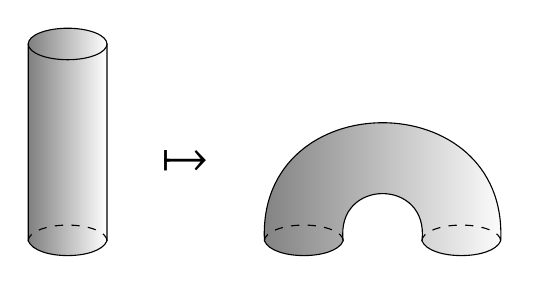
\begin{tikzpicture}
    \identc
    \node [font=\fontsize{18}{18}\selectfont] at (1.5,1) {$\mapsto$};
    \begin{scope}[xshift=4cm]
      \zagc
    \end{scope}  
  \end{tikzpicture}
\end{center}
Similarly, given a Feynman diagram from a set $P$ of particles to a set $Q$, we can ``bend'' the input set around and make it an output, getting a diagram from photons to $Q$ and the antiparticles of $P$:
\begin{center}
  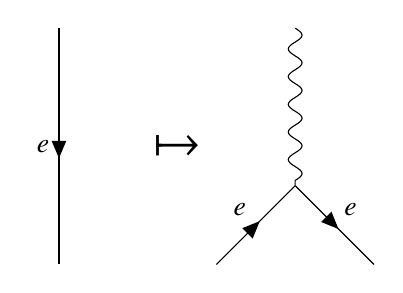
\begin{tikzpicture}
    \coordinate (A) at (1,3);
    \coordinate (D) at (1,0);
    \draw[electron] (A) -- node [left, pos=0.5] {$e$} (D);
    \node [font=\fontsize{18}{18}\selectfont] at (2.5,1.5) {$\mapsto$};
    \coordinate (E) at (4,3);
    \coordinate (F) at (4,1);
    \coordinate (G) at (3,0);
    \coordinate (H) at (5,0);
    \draw[photon] (E) -- (F);
    \draw[electron] (G) -- node [above left, pos=0.5] {$e$} (F);
    \draw[electron] (F) -- node [above right, pos=0.5] {$e$} (H);
  \end{tikzpicture}
\end{center}
Given any linear transformation from a Hilbert space $P$ to a Hilbert space $Q$, we can use the notion of ``gate teleportation'' \cite{GC} to encode the transformation into a quantum state in $P^* \otimes Q.$  When the function type can be expressed in terms of a dual object and the tensor product, as with Feynman diagrams, the category of cobordisms, or Hilbert spaces, we call the category ``compact closed''.

Feynman diagrams were designed to represent quantum systems interacting.  We assign a Hilbert space of quantum states to each particle such that the pairing and braiding operations are preserved: if we assign the space $U$ to one particle and $V$ to another, then we have to assign $U \otimes V$ to the pair of particles.  We assign a linear transformation to each vertex that tells how the quantum states evolve.  This kind of structure-preserving map is called a ``braided monoidal functor''; every monoidal functor also preserves duals, so the entire structure of a compact closed category is preserved.

We can consider such functors from other compact closed categories into the category Hilb of Hilbert spaces and linear transformations.  For example, we can think of manifolds as modeling empty curved space, and cobordisms as modeling spacetime.  A braided monoidal functor from the category of manifolds and cobordisms to Hilb assigns a Hilbert space of quantum states to space and a linear transformation to spacetime, giving a toy model of quantum gravity.  This toy model does not include matter; it only talks about topological changes in space over time, so the model is called a ``topological quantum field theory''.

The structure of a compact closed category can be generalized to ``bicategories'', where in addition to morphisms between objects we have 2-morphisms between morphisms.  In chapter II.2, we lay out the complete definition of a compact closed bicategory (the parts of which have not appeared together in a single place before) and then prove that various useful bicategories are compact closed.  We take special note of bicategories of ``spans''.

In particular, given a category $T$ with pullbacks, we can define a bicategory $\Span(T)$ whose
\begin{itemize}
  \item objects are those of $T$,
  \item morphisms from $A$ to $B$ are ``spans'' consisting of an ``apex'' object $C$ and an ordered pair of morphisms $(f:C\to A, g:C \to B)$ from $T$, and
  \item 2-morphisms are morphisms from $C$ to $C'$ such that the obvious diagram commutes.
\end{itemize}
If $T$ is the category of finite sets, then we can think of the subset of $C$ consisting of those elements $c$ such that $f(c) = a$ and $g(c) = b$ as being a ``matrix element'' at row $a$ and column $b$.  If we simply count these subsets, we get a matrix of natural numbers, and the pullback corresponds to matrix multiplication.  By using categories $T$ other than the category of finite sets, we get a vast generalization of linear algebra.  We conclude chapter II.2 with a proof that when we take the monoidal tricategory of spans described by Hoffnung \cite{Hoffnung} and mod out by 3-isomorphisms, we get a compact closed bicategory.

Compact closed bicategories are interesting to us because they open up at least three areas for future research.  First, Lawvere showed that we can think of categories with products as a kind of programming language.  As programmers, we can write a Java interface that describes the operations on a monoid (identity element and multiplication) and write tests to check the relations (associativity and unit laws).  This interface, together with the tests, is a presentation of a category with products, called ``the Lawvere theory for monoids''.  Every implementation of the interface describes a functor from the Lawvere theory for monoids into the category Set and vice versa.  The tao of categorification suggests there should be a ``higher Lawvere theory of symmetric monoidal closed categories''; the fact that the currying adjunction between tensor and the internal hom is an isomorphism of profunctors means that this higher theory ought to be a compact closed bicategory and take models in Prof.

Second, Lambek and Scott showed that simply-typed lambda calculus forms a cartesian closed category, but only if we {\em ignore the process of computation.}  This is only possible because lambda calculus is confluent: it doesn't matter in what order the rewrite rules are applied.  Concurrent calculi like Milner's pi calculus are not confluent; once we can express contention for resources---like a deposit to and a withdrawal from the same bank account---it matters a great deal in which order the rewrites occur.  This suggests that we need to explicitly account for rewrites using 2-cells in a bicategorical setting.  The higher theory of a symmetric monoidal closed category above provides many of the pieces we need for the pi calculus: the unit object can be the zero process, the tensor product can be concurrency, and the internal hom should be involved in putting a process under a prefix.  The 2-cells for adjunctions in this bicategory drawn as string diagrams look amazingly like synchronization on a name.

Finally, this bicategorical approach should also fit better with physics: rewrites are processes that occur over time like particle interactions do.  Extended topological quantum field theories should be functors between compact closed bicategories, so it's not unreasonable to expect a nice quantum interpretation of some kind of linear pi calculus.

\setcounter{chapter}{0}
\part{Algorithmic information theory}
\chapter{Algorithmic thermodynamics}

The first mathematical structure we will examine that appears in both computer science and physics is the partition function.  Partition functions encode how likely it is to find a system in a given state.  From the partition function, we can compute the ``entropy'', the number of bits required to pick out the particular state the system is in.  In statistical mechanics, the bits describe the positions and momenta of a collection of particles; in algorithmic information theory, the bits describe a program.

Algorithmic entropy can be seen as a special case of entropy as studied in statistical mechanics.  This viewpoint allows us to apply many techniques developed for use in thermodynamics to the subject of algorithmic information theory.  In particular, suppose we fix a universal prefix-free Turing machine and let $X$ be the set of programs that halt for this machine.  Then we can regard $X$ as a set of `microstates', and treat any function on $X$ as an `observable'.  For any collection of observables, we can study the Gibbs ensemble that maximizes entropy subject to constraints on expected values of these observables.  We illustrate this by taking the log runtime, length, and output of a program as observables analogous to the energy $E$, volume $V$ and number of molecules $N$ in a container of gas.  The conjugate variables of these observables allow us to define quantities which we call the `algorithmic temperature' $T$, `algorithmic pressure' $P$ and `algorithmic potential' $\mu$, since they are analogous to the temperature, pressure and chemical potential.  We derive an analogue of the fundamental thermodynamic relation $d E = TdS - P d V + \mu d N$, and use it to study thermodynamic cycles analogous to those for heat engines.  We also investigate the values of $T, P$ and $\mu$ for which the partition function converges. At some points on the boundary of this domain of convergence, the partition function becomes uncomputable.  Indeed, at these points the partition function itself has nontrivial algorithmic entropy.

\section{Introduction}\label{intro}

Many authors \cite{BGLVZ, Chaitin1975, FT1982, Kolmogorov1965, LevinZvonkin, Solomonoff1964, Szilard1929, Tadaki2008} have discussed the analogy between algorithmic entropy and entropy as defined in statistical mechanics: that is, the entropy of a probability measure $p$ on a set $X$.  It is perhaps insufficiently appreciated that algorithmic entropy can be seen as a \textit{special case} of the entropy as defined in statistical mechanics.  We describe how to do this in Section \ref{entropy}.

This allows all the basic techniques of thermodynamics to be imported to algorithmic information theory.  The key idea is to take $X$ to be some version of `the set of all programs that eventually halt and output a natural number', and let $p$ be a Gibbs ensemble on $X$.  A
Gibbs ensemble is a probability measure that maximizes entropy subject to constraints on the mean values of some observables --- that is, real-valued functions on $X$.

In most traditional work on algorithmic entropy, the relevant observable is the length of the program.  However, much of the interesting structure of thermodynamics only becomes visible when we consider several observables.  When $X$ is the set of programs that halt and output a natural number, some other important observables include the output of the program and logarithm of its runtime.  So, in Section \ref{thermodynamics} we illustrate how ideas from thermodynamics can be applied to algorithmic information theory using these three observables.  

To do this, we consider a Gibbs ensemble of programs which maximizes entropy subject to constraints on:
\begin{itemize}
\item
$E$, the expected value of the logarithm of the program's runtime (which we treat as analogous to the energy of a container of gas),
\item 
$V$, the expected value of the length of the program (analogous to the volume of the container), and 
\item
$N$, the expected value of the program's output (analogous to the number of molecules in the gas).
\end{itemize}
This measure is of the form
\[       p = \frac{1}{Z} e^{-\beta E(x) -\gamma V(x) - \delta N(x)} \]
for certain numbers $\beta, \gamma, \delta$, where the normalizing factor
\[     Z = \sum_{x \in X} e^{-\beta E(x) -\gamma V(x) - \delta N(x)} \]
is called the `partition function' of the ensemble.  The partition function reduces to Chaitin's number $\Omega$ when $\beta = 0$, $\gamma = \ln 2$ and $\delta = 0$.  This number is uncomputable \cite{Chaitin1975}.  However, we show that the partition function $Z$ is computable when $\beta > 0$, $\gamma \ge \ln 2$, and $\delta \ge 0$.

We derive an algorithmic analogue of the basic thermodynamic relation
\[          dE = T dS - P dV + \mu dN . \]
Here:
\begin{itemize}
\item 
$S$ is the entropy of the Gibbs ensemble,
\item
$T = 1/\beta$ is the `algorithmic temperature' (analogous to the temperature of a container of gas).  Roughly speaking, this counts how many times you must double the runtime in order to double the number of programs in the ensemble while holding their mean length and output fixed.
\item
$P = \gamma/\beta$ is the `algorithmic pressure' (analogous to pressure).  This measures the tradeoff between runtime and length. Roughly speaking, it counts how much you need to decrease the mean length to increase the mean log runtime by a specified amount, while holding the number of programs in the ensemble and their mean output fixed.
\item
$\mu = -\delta/\beta$ is the `algorithmic potential' (analogous to chemical potential).  Roughly speaking, this counts how much the mean log runtime increases when you increase the mean output while holding the number of programs in the ensemble and their mean length fixed.
\end{itemize}

Starting from this relation, we derive analogues of Maxwell's relations and consider thermodynamic cycles such as the Carnot cycle or Stoddard cycle.  For this we must introduce concepts of `algorithmic heat' and `algorithmic work'.

\begin{center}
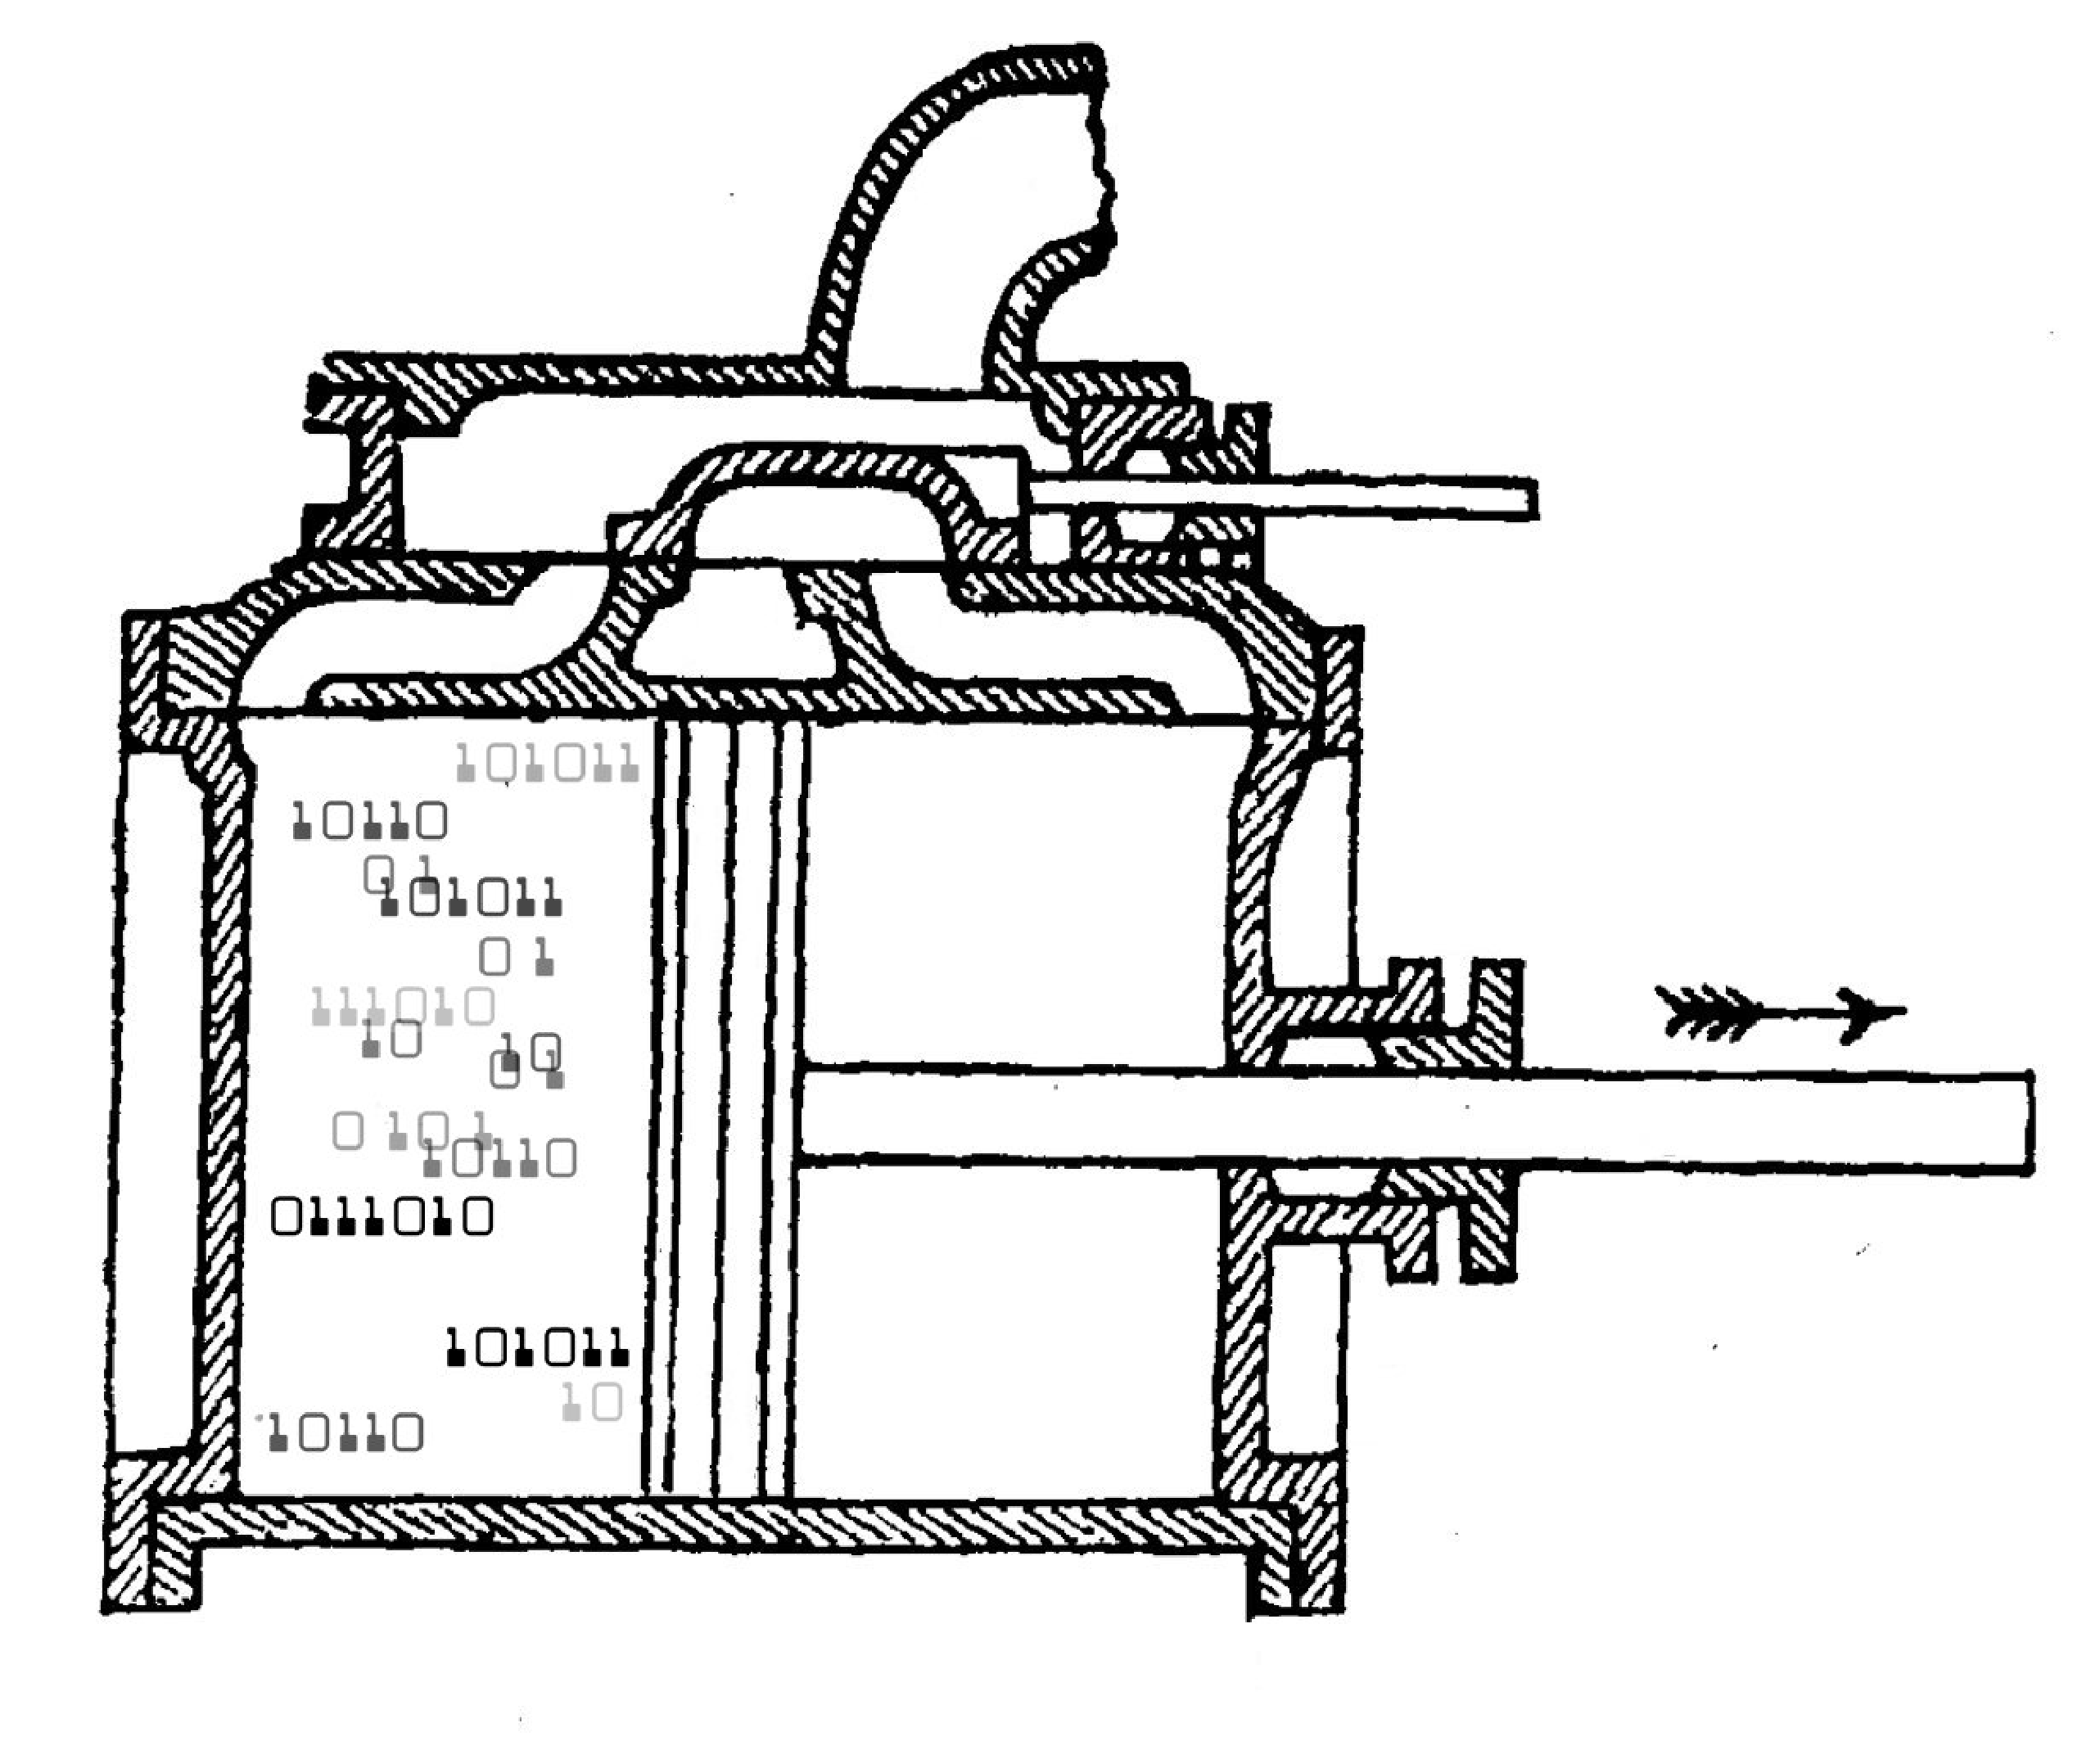
\includegraphics[scale=0.15, angle=0.3]{piston.eps}
\end{center}

Charles Babbage described a computer powered by a steam engine;
we describe a heat engine powered by programs!  We admit that the significance of this line of thinking remains a bit mysterious.  However, we hope it points the way toward a further synthesis of algorithmic information theory and thermodynamics. We call this hoped-for synthesis `algorithmic thermodynamics'.

\section{Related Work}

Li and Vit\'anyi use the term `algorithmic thermodynamics' for describing physical states using a universal prefix-free Turing machine $U$. They look at the smallest program $p$ that outputs a description $x$ of a particular microstate to some accuracy, and define the physical entropy to be
\[ S_A(x) = (k \ln 2)(K (x) + H_x), \]
where $K(x) = |p|$ and $H_x$ embodies the uncertainty in the actual state given $x$. They summarize their own work and subsequent work by others in chapter eight of their book \cite{LV}.  Whereas they consider $x=U(p)$ to be a microstate, we consider $p$ to be the microstate and $x$ the value of the observable $U$.  Then their observables $O(x)$ become observables of the form $O(U(p))$ in our model.
 
Tadaki \cite{Tadaki2002} generalized Chaitin's number $\Omega$ to a function 
$\Omega^D$ and showed that the value of this function is compressible by a factor of exactly $D$ when $D$ is computable. Calude and Stay \cite{CSNatural2006} pointed out that this generalization was formally equivalent to the partition function of a statistical mechanical system where temperature played the role of the compressibility factor, and studied various observables of such a system. Tadaki \cite{Tadaki2008} then explicitly constructed a system with that partition function: given a total length $E$ and number of programs
$N,$ the entropy of the system is the log of the number of $E$-bit strings in $\dom(U)^N.$  The temperature is
\[ \frac{1}{T} = \left.\frac{\Delta E}{\Delta S}\right|_N. \]
In a follow-up paper \cite{Tadaki2009}, Tadaki showed that various other quantities like the free energy shared the same compressibility properties as $\Omega^D$.  In this thesis, we consider multiple variables, which is necessary for thermodynamic cycles, chemical reactions, and so forth.

Manin and Marcolli \cite{MM2009} derived similar results in a broader context and studied phase transitions in those systems.  Manin \cite{ManinRenorm1, ManinRenorm2}
also outlined an ambitious program to treat the infinite runtimes one finds in undecidable problems as singularities to be removed through the process of renormalization.  In a manner reminiscent of hunting for the proper definition of the 
``one-element field'' $F_{un},$ he collected ideas from many different places and considered how they all touch on this central theme. While he mentioned a runtime cutoff as being analogous to an energy cutoff, the renormalizations he presented are uncomputable.  In this thesis, we take the log of the runtime as being analogous to the energy; the randomness described by Chaitin and Tadaki then arises as the infinite-temperature limit.

\section{Algorithmic Entropy}\label{entropy}

To see algorithmic entropy as a special case of the entropy of a probability measure, it is useful to follow Solomonoff
\cite{Solomonoff1964} and take a Bayesian viewpoint.  In Bayesian probability theory, we always start with a probability measure called a `prior', which describes our assumptions about the situation at hand before we make any further observations. As we learn more, we may update this prior.  This approach suggests that we should define the entropy of a probability measure
\textit{relative to another probability measure} --- the prior.

A probability measure $p$ on a finite set $X$ is simply a function $p
\maps X \to [0,1]$ whose values sum to 1, and its entropy is defined as follows:
\[  S(p) = -\sum_{x \in X} p(x) \ln p(x)  .\]
But we can also define the entropy of $p$ relative to another probability measure $q$:
\[  S(p,q) = -\sum_{x \in X} p(x) \ln\frac{p(x)}{q(x)} \raisebox{0.4ex}{.}\]
This {\bf relative entropy} has been extensively studied and goes by various other names, including `Kullback--Leibler divergence' \cite{KL}
and `information gain' \cite{Renyi}.  

The term `information gain' is nicely descriptive.  Suppose we initially assume the outcome of an experiment is distributed according to the probability measure $q$.  Suppose we then repeatedly do the experiment and discover its outcome is distributed according to the measure $p$. Then the information gained is $S(p,q)$.

Why?  We can see this in terms of coding.  Suppose $X$ is a finite set of signals which are randomly emitted by some source. Suppose we wish to encode these signals as efficiently as possible in the form of bit strings.  Suppose the source emits the signal $x$ with probability $p(x)$, but we erroneously believe it is emitted with probability $q(x)$.  Then $S(p,q)/\ln 2$ is the expected extra message-length per signal that is required if we use a code that is optimal for the measure $q$ instead of a code that is optimal for the true measure, $p$.

The ordinary entropy $S(p)$ is, up to a constant, just the relative entropy in the special case where the prior assigns an equal probability to each outcome.  In other words:
\[  S(p) = S(p,q_0) + S(q_0)  \]
when $q_0$ is the so-called `uninformative prior', with $q_0(x) =
1/|X|$ for all $x \in X$.  

We can also define relative entropy when the set $X$ is countably infinite.  As before, a probability measure on $X$ is a function $p
\maps X \to [0,1]$ whose values sum to 1.  And as before, if $p$ and
$q$ are two probability measures on $X$, the entropy of $p$ relative to $q$ is defined by
\begin{equation}
\label{relative_entropy}
  S(p,q) = -\sum_{x \in X} p(x) \, \ln\frac{p(x)}{q(x)} \raisebox{0.4ex}{.}
\end{equation} 
But now the role of the prior becomes more clear, because there is no probability measure that assigns the same value to each outcome!

In what follows we will take $X$ to be --- roughly speaking --- the set of all programs that eventually halt and output a natural number.  As we shall see, while this set is countably infinite, there are still some natural probability measures on it, which we may take as priors.

To make this precise, we recall the concept of a universal prefix-free Turing machine.  In what follows we use {\bf string} to mean a bit string, that is, a finite, possibly empty, list of 0's and
1's.  If $x$ and $y$ are strings, let $x||y$ be the concatenation of
$x$ and $y.$ A \textbf{prefix} of a string $z$ is a substring beginning with the first letter, that is, a string $x$ such that $z =
x||y$ for some $y$.  A \textbf{prefix-free} set of strings is one in which no element is a prefix of any other.  The \textbf{domain}
$\dom(M)$ of a Turing machine $M$ is the set of strings that cause $M$
to eventually halt.  We call the strings in $\dom(M)$
\textbf{programs}.  We assume that when the $M$ halts on the program
$x$, it outputs a natural number $M(x)$.  Thus we may think of the machine $M$ as giving a function $M \maps \dom(M) \to \N$.

A \textbf{prefix-free Turing machine} is one whose halting programs form a prefix-free set.  A prefix-free machine $U$ is {\bf universal}
if for any prefix-free Turing machine $M$ there exists a constant
$c$ such that for each string $x$, there exists a string $y$ with
\[ U(y) = M(x) \; \mbox{ and } \; |y| < |x| + c. \]

Let $U$ be a universal prefix-free Turing machine.  Then we can define some probability measures on $X = \dom(U)$
as follows.   Let 
\[  |\cdot | \maps X \to \N \]
be the function assigning to each bit string its length. Then there is for any constant $\gamma \ge \ln 2$ a probability measure 
$p$ given by
\[   p(x) = \frac{1}{Z} e^{-\gamma |x|}. \]
Here the normalization constant $Z$ is chosen to make the numbers
$p(x)$ sum to 1:
\[   Z = \sum_{x \in X} e^{-\gamma |x|}  .\]
It is worth noting that for computable real numbers $\gamma \ge \ln 2$, the normalization constant $Z$ is uncomputable \cite{Tadaki2002}. Indeed, when $\gamma = \ln 2$, $Z$ is Chaitin's famous number $\Omega$. We return to this issue in Section \ref{computability}.

Let us assume that each program prints out some natural number as its output.   Thus we have a function
\[ N \maps X \to \N \]
where $N(x)$ equals $i$ when program $x$ prints out the number $i$. We may use this function to `push forward' $p$ to a probability measure
$q$ on the set $\N$.  Explicitly:
\[ 
   q(i) = \displaystyle {\sum_{x \in X : N(x) = i}} e^{-\gamma |x|} \; .
\]
In other words, if $i$ is some natural number, $q(i)$ is the probability that a program randomly chosen according to the measure
$p$ will print out this number.  

Given any natural number $n$, there is a probability measure
$\delta_n$ on $\N$ that assigns probability 1 to this number:
\[   \delta_n(m) = \left\{ \begin{array}{cl} 1 & \textrm{if } m = n \\
                              0 & \textrm{otherwise.}  
           \end{array} \right.
\]
We can compute the entropy of $\delta_n$ relative to $q$:
\begin{equation}
\label{relative.entropy}
\begin{array}{ccl} S(\delta_n,q) &=& 
\displaystyle{ -\sum_{i \in \N}  \delta_n(i) \, 
\ln \frac{\delta_n(i)}{q(i)}}   \\
\\ &=& \displaystyle{ -\ln \left( \sum_{x \in X \colon N(x) = n} 
e^{-\gamma |x|} \right) + \ln Z .}  \\
\end{array}
\end{equation}
Since the quantity $\ln Z$ is independent of the number $n$, and uncomputable, it makes sense to focus attention on the other part of the relative entropy:
\[  \displaystyle{ -\ln \left( \sum_{x \in X \colon N(x) = n} 
e^{-\gamma |x|} \right) .}  
\]
If we take $\gamma = \ln 2$, this is precisely the \textbf{algorithmic entropy} \cite{Chaitin1976,LevinZvonkin} of the number $n$.  So, up to the additive constant $\ln Z$, we have seen that \textit{algorithmic entropy is a special case of relative entropy}.  

One way to think about entropy is as a measure of surprise: if you can predict what comes next --- that is, if you have a program that can compute it for you --- then you are not surprised.  For example, the first 2000 bits of the binary fraction for 1/3 can be produced with this short Python program:
\begin{center}
  {\tt print "01" * 1000}
\end{center}
But if the number is complicated, if every bit is surprising and unpredictable, then the shortest program to print the number does not do any computation at all! It just looks something like
\begin{center}
  {\tt print "101000011001010010100101000101111101101101001010"}
\end{center}
Levin's coding theorem \cite{Levin1974} says that the difference between the algorithmic entropy of a number and its \textbf{Kolmogorov complexity} --- the length of the shortest program that outputs it
--- is bounded by a constant that only depends on the programming language.

So, up to some error bounded by a constant, \textit{algorithmic information is information gain}.  The algorithmic entropy is the information gained upon learning a number, if our prior assumption was that this number is the output of a randomly chosen program ---
randomly chosen according to the measure $p$ where $\gamma = \ln 2$.

So, algorithmic entropy is not just \textit{analogous} to entropy as defined in statistical mechanics: it is a \textit{special case}, as long as we take seriously the Bayesian philosophy that entropy should be understood as relative entropy.  This realization opens up the possibility of taking many familiar concepts from thermodynamics, expressed in the language of statistical mechanics, and finding their counterparts in the realm of algorithmic information theory.

But to proceed, we must also understand more precisely the role of the measure $p$.  In the next section, we shall see that this type of measure is already familiar in statistical mechanics: it is a Gibbs ensemble.

\section{Algorithmic Thermodynamics}\label{thermodynamics}

Suppose we have a countable set $X$, finite or infinite, and suppose $C_1, \dots, C_n \maps X \to \R$ is some collection of functions.  Then we may seek a probability measure $p$
that maximizes entropy subject to the constraints that the mean value of each observable $C_i$ is a given real number $\overline{C}_i$:
\[            \sum_{x \in X} p(x) \, C_i(x) = \overline{C}_i  .\]
As nicely discussed by Jaynes \cite{Jaynes1957,Jaynes2003}, the solution, if it exists, is the so-called {\bf Gibbs ensemble}:
\[             p(x) = \frac{1}{Z} e^{-(s_1 C_1(x) + \cdots + s_n C_n(x))}  \]
for some numbers $s_i \in \R$ depending on the desired mean values 
$\overline{C}_i$.  Here the normalizing factor $Z$ is called the 
{\bf partition function}:
\[             Z = \sum_{x \in X} e^{-(s_1 C_1(x) + \cdots + s_n C_n(x))} 
\;.  \]

In thermodynamics, $X$ represents the set of {\bf microstates} of some physical system.  A probability measure on $X$ is also known as an
{\bf ensemble}.  Each function $C_i \maps X \to \R$ is called an {\bf observable}, and the corresponding quantity $s_i$ is called the {\bf conjugate variable} of that observable.  For example, the conjugate of the energy $E$ is the inverse of temperature $T$, in units where Boltzmann's constant equals 1.  The conjugate of the volume $V$ --- of a piston full of gas, for example --- is the pressure $P$ divided by the temperature.  And in a gas containing molecules of various types, the conjugate of the number $N_i$ of molecules of the $i$th type is minus the `chemical potential' $\mu_i$, again divided by temperature. For easy reference, we list these observables and their conjugate variables below.

\begin{center}
\renewcommand{\arraystretch}{2.3}
\begin{tabular}{c|c}  
\multicolumn{2}{c}{\bf{THERMODYNAMICS}} \\
\hline Observable    &  Conjugate Variable\\ 
\hline energy: $E$   &  $\displaystyle{\frac{1}{T}}$ \\
volume: $V$   &  $\displaystyle{\frac{P}{T}}$  \\
number: $N_i$ &  $\displaystyle{-\frac{\mu_i}{T}}$   \\
\end{tabular}
\end{center}
\renewcommand{\arraystretch}{1}

Now let us return to the case where $X=\dom(U)$.  Recalling that programs are bit strings, one important observable for programs is the length:
\[  |\cdot | \maps X \to \N .\]
We have already seen the measure
\[   p(x) = \frac{1}{Z} e^{-\gamma |x|} .\]
Now its significance should be clear!   This is the probability measure on programs that maximizes entropy subject to the constraint that the mean length is some constant $\ell$:
\[    \sum_{x \in X}  p(x) \, |x| = \ell .  \]
So, $\gamma$ is the conjugate variable to program length.

There are, however, other important observables that can be defined for programs, and each of these has a conjugate quantity.  To make the analogy to thermodynamics as vivid as possible, let us arbitrarily choose two more observables and treat them as analogues of energy and the number of some type of molecule.  Two of the most obvious observables are `output' and `runtime'.  Since Levin's computable complexity measure \cite{Levin1973} uses the logarithm of runtime as a kind of `cutoff' reminiscent of an energy cutoff in renormalization, we shall arbitrarily choose the log of the runtime to be analogous to the energy, and denote it as
\[    E \maps X \to [0,\infty) \]
Following the chart above, we use $1/T$ to stand for the variable conjugate to $E$.   We arbitrarily treat the output of a program as analogous to the number of a certain kind of molecule, and denote it as
\[    N \maps X \to \N . \]
We use $-\mu/T$ to stand for the conjugate variable of $N$. Finally, as already hinted, we denote program length as
\[    V \maps X \to \N   \]
so that in terms of our earlier notation, $V(x) = |x|$.  We use
$P/T$ to stand for the variable conjugate to $V$.

\begin{center}
\renewcommand{\arraystretch}{2.3}
\begin{tabular}{c|c}  
\multicolumn{2}{c}{\bf{ALGORITHMS}} \\
\hline Observable  & Conjugate Variable\\ 
\hline log runtime: $E$  & $\displaystyle{\frac{1}{T}}$ \\
length:      $V$  & $\displaystyle{\frac{P}{T}}$  \\
output:      $N$  & $\displaystyle{-\frac{\mu}{T}}$   \\
\end{tabular}
\end{center}
\renewcommand{\arraystretch}{1}

Before proceeding, we wish to emphasize that the analogies here were chosen somewhat arbitrarily.  They are merely meant to illustrate the application of thermodynamics to the study of algorithms.  There may or may not be a specific `best' mapping between observables for programs and observables for a container of gas!  Indeed, Tadaki \cite{Tadaki2008} has explored another analogy, where length rather than log run time is treated as the analogue of energy.  There is nothing wrong with this.  However, he did not introduce enough other observables to see the whole structure of thermodynamics, as developed in Sections \ref{elementary}-\ref{cycles}
below.  

Having made our choice of observables, we define the partition function by 
\[     Z = \sum_{x \in X} e^{-\frac{1}{T}(E(x) + P V(x) - \mu N(x))} \; .\]
When this sum converges, we can define a probability measure on $X$, the Gibbs ensemble, by
\[    p(x) = \frac{1}{Z} e^{-\frac{1}{T}(E(x) + P V(x) - \mu N(x))} \; .\]
Both the partition function and the probability measure are functions of $T, P$ and $\mu$.  From these we can compute the mean values of the observables to which these variables are conjugate:
\[
\begin{array}{ccc} 
    \overline{E} &=& \displaystyle{\sum_{x \in X}} p(x) \, E(x)   \\
                                                   \\
    \overline{V} &=& \displaystyle{\sum_{x \in X}} p(x) \, V(x)   \\
                                                   \\
    \overline{N} &=& \displaystyle{\sum_{x \in X}} p(x) \, N(x)   
\end{array}
\]
In certain ranges, the map $(T,P,\mu) \mapsto (\overline{E},
\overline{V}, \overline{N})$ will be invertible.  This allows us to alternatively think of $Z$ and $p$ as functions of $\overline{E}, \overline{V},$ and $\overline{N}$. In this situation it is typical to abuse language by omitting the overlines which denote `mean value'.

\subsection{Elementary Relations} \label{elementary}

The entropy $S$ of the Gibbs ensemble is given by
\[      S = - \sum_{x \in X} p(x)\, \ln p(x) .\]
We may think of this as a function of $T, P$ and $\mu$, or alternatively --- as explained above --- as functions of the mean values $E, V,$ and $N$.  Then simple calculations, familiar from statistical mechanics \cite{Reif}, show that
%see Reif eqs.\ 8.7.4 to 8.7.5

\begin{equation}
\label{derivative1}
\displaystyle{\left.\frac{\partial S}{\partial E}\right|_{V,N}}  =
\displaystyle{\frac{1}{T}} 
\end{equation}

\begin{equation}
\label{derivative2}
\displaystyle{\left.\frac{\partial S}{\partial V}\right|_{E,N}}  =
\displaystyle{\frac{P}{T}} 
\end{equation}

\begin{equation}
\label{derivative3}
\displaystyle{\left.\frac{\partial S}{\partial N}\right|_{E,V}}  =
-\displaystyle{\frac{\mu}{T}} .
\end{equation}
We may summarize all these by writing
%see Reif eqs.\ 8.7.6 and 8.7.8
\[            dS = \frac{1}{T} dE + \frac{P}{T} dV - \frac{\mu}{T} dN  \]
or equivalently
\begin{equation}
\label{differentials}
          dE = T dS - P dV + \mu dN  .
\end{equation}
Starting from the latter equation we see:
\begin{equation}
\label{derivatives1}
\displaystyle{\left.\frac{\partial E}{\partial S}\right|_{V,N}}  =
\displaystyle{T} 
\end{equation}

\begin{equation}
\label{derivatives2}
\displaystyle{\left.\frac{\partial E}{\partial V}\right|_{S,N}} =
\displaystyle{-P}
\end{equation}

\begin{equation}
\label{derivatives3}
\displaystyle{\left.\frac{\partial E}{\partial N}\right|_{S,V}}  =
\displaystyle{\mu} .
\end{equation}

With these definitions, we can start to get a feel for what the conjugate variables are measuring.  To build intuition, it is useful to think of the entropy $S$ as roughly the logarithm of the number of programs whose log runtimes, length and output lie in small ranges $E
\pm \Delta E$, $V \pm \Delta V$ and $N \pm \Delta N$. This is at best approximately true, but in ordinary thermodynamics this approximation is commonly employed and yields spectacularly good results.  That is why in thermodynamics people often say the entropy is the logarithm of the number of microstates for which the observables $E, V$ and $N$ lie within a small range of their specified values \cite{Reif}.

If you allow programs to run longer, more of them will halt and give an answer.  The \textbf{algorithmic temperature}, $T$, is roughly the number of times you have to double the runtime in order to double the number of ways to satisfy the constraints on length and output.

The \textbf{algorithmic pressure}, $P$, measures the tradeoff between runtime and length \cite{CSHalting2006}: if you want to keep the number of ways to satisfy the constraints constant, then the freedom gained by having longer runtimes has to be counterbalanced by shortening the programs. This is analogous to the pressure of gas in a piston: if you want to keep the number of microstates of the gas constant, then the freedom gained by increasing its energy has to be counterbalanced by decreasing its volume.  

Finally, the \textbf{algorithmic potential} describes the relation between log runtime and output: it is a quantitative measure of the principle that most large outputs must be produced by long programs.

\subsection{Thermodynamic Cycles} \label{cycles}

One of the first applications of thermodynamics was to the analysis of heat engines.  The underlying mathematics applies equally well to algorithmic thermodynamics.  Suppose $C$ is a loop in $(T,P,\mu)$ 
space.  Assume we are in a region that can also be coordinatized by the variables $E,V,N$.  Then the change in {\bf algorithmic heat} 
around the loop $C$ is defined to be
\[        \Delta Q = \oint_C T dS  .\]
Suppose the loop $C$ bounds a surface $\Sigma$.  Then Stokes' theorem implies that
\[        \Delta Q = \oint_C T dS  = \int_{\Sigma} dT dS . \]
However, Equation (\ref{differentials}) implies that
\[    dT dS = d(T dS) = d(dE + P dV - \mu dN) = + dP dV - d\mu dN \]
since $d^2 = 0$.  So, we have
\[      \Delta Q = \int_{\Sigma} (dP dV - d\mu dN)  \]
or using Stokes' theorem again
\begin{equation}
\label{loop}
      \Delta Q = \int_C (P dV - \mu dN). 
\end{equation}

In ordinary thermodynamics, $N$ is constant for a heat engine using gas in a sealed piston.  In this situation we have
\[
      \Delta Q = \int_C P dV  .
\]
This equation says that the change in heat of the gas equals the work done on the gas --- or equivalently, minus the work done \emph{by} the gas.  So, in algorithmic thermodynamics, let us define $\int_C P dV$
to be the {\bf algorithmic work} done on our ensemble of programs as we carry it around the loop $C$.  Beware: the algorithmic work has the same units as the observable we choose to play the role of internal energy.  The algorithmic work is only the same as the `computational work', meaning the amount of computation done by a program as it runs, if we choose to use the runtime as the analogue of internal energy. We have chosen to use the log runtime instead, so the concepts are related, but not the same.  If we had chosen to use the length of a program to represent the internal energy, then algorithmic work would be measured in bits and the two concepts would be completely distinct.

To see an example of a cycle in algorithmic thermodynamics, consider the analogue of the heat engine patented by Stoddard in 1919
\cite{Stoddard1919}.  Here we fix $N$ to a constant value and consider the following loop in the $PV$ plane:
\begin{center}
  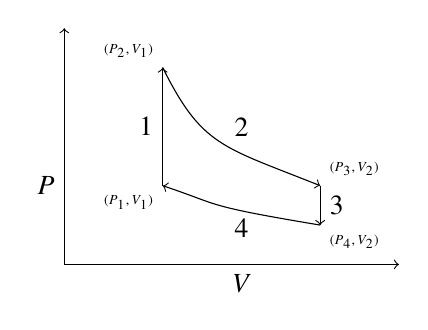
\begin{tikzpicture}
    \draw [->] (-.25,1)--(-.25,4);
    \draw [->] (-.25,1)--(4,1);
    \draw [->] (1,2)--(1,3.5);
    \draw [->] (1,3.5) .. controls (1.5, 2.5) and (1.75, 2.5) .. (3,2);
    \draw [->] (3,2)--(3,1.5);
    \draw [->] (3,1.5).. controls (1.5,1.75) and (1.75, 1.75) .. (1,2);
    \node at (-.25,2) [left] {$P$};
    \node at (2,1) [below] {$V$};
    \node at (1,2.75) [left] {1};
    \node at (2,2.5) [above] {2};
    \node at (3,1.75) [right] {3};
    \node at (2,1.7) [below] {4};
    \begin{scope}[font=\fontsize{5}{5}\selectfont]
      \node at (1,2) [below left] {$(P_1, V_1)$};
      \node at (1,3.5) [above left] {$(P_2, V_1)$};
      \node at (3,2) [above right] {$(P_3, V_2)$};
      \node at (3,1.5) [below right] {$(P_4, V_2)$};
    \end{scope}
  \end{tikzpicture}
\end{center}
We start with an ensemble with algorithmic pressure $P_1$ and mean length $V_1$.  We then trace out a loop built from four parts:

\begin{enumerate}
  \item 
  \emph{Isometric}. We increase the pressure from $P_1$ to $P_2$ while keeping
  the mean length constant.  No algorithmic work is done on the ensemble
  of programs during this step.
  \item
  \emph{Isentropic.} We increase the length from $V_1$ to $V_2$ while keeping
  the number of halting programs constant.  High pressure means 
  that we're operating in a range of runtimes where if we increase
  the length a little bit, many more programs halt.  In order
  to keep the number of halting programs constant,
  we need to shorten the runtime significantly.  As we gradually
  increase the length and lower the runtime, the pressure drops to $P_3$.
  The total difference in log runtime is the algorithmic 
  work done on the ensemble during this step.
  \item
  \emph{Isometric.} Now we decrease the pressure from $P_3$ to $P_4$ while
  keeping the length constant.  No algorithmic work is done during this step.
  \item
  \emph{Isentropic.} Finally, we decrease the length from $V_2$ back to $V_1$
  while keeping the number of halting programs constant.
  Since we're at low pressure, we need only increase the
  runtime a little.  As we gradually decrease the length
  and increase the runtime, the pressure rises slightly
  back to $P_1$.  The total increase in log runtime is minus the algorithmic
  work done on the ensemble of programs during this step.
\end{enumerate}
The total algorithmic work done on the ensemble per cycle is the difference in log runtimes between steps 2 and 4.

\subsection{Further Relations} \label{maxwell}

From the elementary thermodynamic relations in Section 
\ref{elementary}, we can derive various others. For example, the so-called `Maxwell relations' are obtained by computing the second derivatives of thermodynamic quantities in two different orders and then applying the basic derivative relations, Equations (\ref{derivatives1}-\ref{derivatives3}).  While trivial to prove, these relations say some things about algorithmic thermodynamics which may not seem intuitively obvious.

We give just one example here.  Since mixed partials commute, we have:
\[  \left.\frac{\partial^2 E}{\partial V \partial S}\right|_N = 
\left.\frac{\partial^2 E}{\partial S \partial V}\right|_N . \]
Using Equation (\ref{derivatives1}), the left side can be computed as follows:
\[  \left.\frac{\partial^2 E}{\partial V \partial S}\right|_N = 
\left.\frac{\partial}{\partial V}\right|_{S,N}
\left.\frac{\partial E}{\partial S}\right|_{V,N} = 
\left.\frac{\partial T}{\partial V}\right|_{S,N}  \]
Similarly, we can compute the right side with the help of Equation (\ref{derivatives2}):
\[  \left.\frac{\partial^2 E}{\partial S \partial V}\right|_N = 
\left.\frac{\partial}{\partial S}\right|_{V,N}
\left.\frac{\partial E}{\partial V}\right|_{S,N} = 
-\left.\frac{\partial P}{\partial S}\right|_{V,N} . \]
As a result, we obtain:
\[  \left.\frac{\partial T}{\partial V}\right|_{S,N}  =
-\left.\frac{\partial P}{\partial S}\right|_{V,N} . \]

We can also derive interesting relations involving derivatives of the partition function.  These become more manageable if we rewrite the partition function in terms of the conjugate variables of the observables $E, V$, and $N$:
\begin{equation}
\label{new.variables}
   \beta = \frac{1}{T}\raisebox{0.4ex}{,} \quad
 \gamma =  \frac{P}{T}\raisebox{0.4ex}{,}  \quad
\delta = -\frac{\mu}{T}\raisebox{0.4ex}.
\end{equation}
Then we have
\[     Z = \sum_{x \in X} e^{-\beta E(x) -\gamma V(x) - \delta N(x)} \]

Simple calculations, standard in statistical mechanics 
\cite{Reif}, then allow us to compute the mean values of observables as derivatives of the logarithm of $Z$ 
with respect to their conjugate variables.    Here let us revert to using overlines to denote mean values:
\[
\begin{array}{ccc}
   \overline{E} &= 
   \displaystyle{\sum_{x \in X} p(x) \, E(x)} &=
- \displaystyle{\frac{\partial}{\partial \beta} \ln Z}  \\  
\\
   \overline{V} &=
   \displaystyle{\sum_{x \in X} p(x) \, V(x)} &=
- \displaystyle{\frac{\partial}{\partial \gamma} \ln Z}  \\  
\\
   \overline{N} &=
   \displaystyle{\sum_{x \in X} p(x) \, N(x)} &=
- \displaystyle{\frac{\partial}{\partial \delta} \ln Z}  
\end{array}
\]
We can go further and compute the variance of these observables using second derivatives:
\[       
\begin{array}{ccc}
   {(\Delta E)^2} &=
\displaystyle{\sum_{x \in X} p(x) (E(x)^2 - \overline{E}^2)} &=
\displaystyle{ \frac{\partial^2}{\partial^2 \beta} \ln Z } 
\end{array}
\]
and similarly for $V$ and $N$.  Higher moments of $E, V$ and 
$N$ can be computed by taking higher derivatives of $\ln Z$.  

\subsection{Convergence}

So far we have postponed the crucial question of convergence:
for which values of $T,P$ and $\mu$ does the partition function 
$Z$ converge?  For this it is most convenient to treat $Z$ as a function of the variables $\beta, \gamma$ and $\delta$
introduced in Equation (\ref{new.variables}).  For which values of $\beta, \gamma$ and $\delta$ does the partition function converge?   

First, when $\beta = \gamma = \delta = 0,$ the contribution of each program is 1.   Since there are infinitely many halting programs, $Z(0,0,0)$ does not converge.

Second, when $\beta = 0, \gamma = \ln 2,$ and $\delta = 0,$ the partition function converges to Chaitin's number
\[ \Omega = \sum_{x \in X} 2^{-V(x)}.  \]
To see that the partition function converges in this case, consider this mapping of strings to segments of the unit interval: 
\begin{center}
  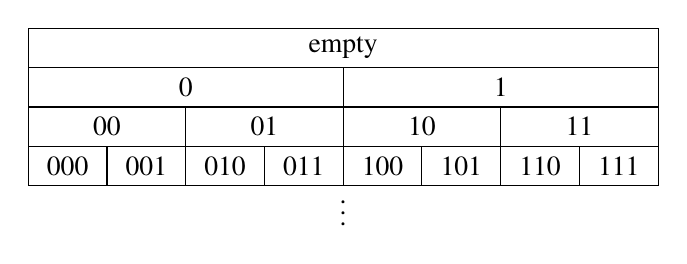
\begin{tikzpicture}
    \draw (0,2)--(0,0);
    \draw (8,2)--(8,0);
    \draw (4,1.5)--(4,0);
    \draw (2,1)--(2,0);
    \draw (6,1)--(6,0);
    \draw (1,.5)--(1,0);
    \draw (3,.5)--(3,0);
    \draw (5,.5)--(5,0);
    \draw (7,.5)--(7,0);
    \node at (4,1.75) {empty};
    \node at (2,1.25) {0};
    \node at (6,1.25) {1};
    \node at (1,0.75) {00};
    \node at (3,0.75) {01};
    \node at (5,0.75) {10};
    \node at (7,0.75) {11};
    \node at (0.5,.25) {000};
    \node at (1.5,.25) {001};
    \node at (2.5,.25) {010};
    \node at (3.5,.25) {011};
    \node at (4.5,.25) {100};
    \node at (5.5,.25) {101};
    \node at (6.5,.25) {110};
    \node at (7.5,.25) {111};
    \node at (4,-0.25) {$\vdots$};
    \foreach \y in {0,1,2,3,4} \draw (0,\y/2)--(8,\y/2);
  \end{tikzpicture}
\end{center}

Each segment consists of all the real numbers whose binary expansion begins with that string; for example, the set of real numbers whose binary expansion begins $0.101\ldots$
is [0.101, 0.110) and has measure $2^{-|101|} = 2^{-3} = 1/8.$
Since the set of halting programs for our universal machine is prefix-free, we never count any segment more than once, so the sum of all the segments corresponding to halting programs is at most 1.

Third, Tadaki has shown \cite{Tadaki2002} that the expression  
\[ \sum_{x \in X} e^{-\gamma V(x)} \]
converges for $\gamma \ge \ln 2$ but diverges for $\gamma < \ln 2.$ 
It follows that $Z(\beta, \gamma, \delta)$
converges whenever $\gamma \ge \ln 2$ and $\beta, \delta \ge 0$.  

Fourth, when $\beta>0$ and $\gamma=\delta=0,$ convergence depends on the machine.  There are machines where infinitely many programs halt immediately.  For these, $Z(\beta,0,0)$ does not converge. However, there are also machines where program $x$ takes at least 
$V(x)$ steps to halt; for these machines $Z(\beta,0,0)$ will converge when $\beta \ge \ln 2.$  Other machines take much longer to run. For these, $Z(\beta,0,0)$ will converge for even smaller values of $\beta$.  

Fifth and finally, when $\beta = \gamma = 0$ and $\delta > 0$, 
$Z(\beta,\gamma,\delta)$ fails to converge, since there are infinitely many programs that halt and output 0.

\subsection{Computability} \label{computability}

Even when the partition function $Z$ converges, it may not be computable.  The theory of computable real numbers was independently introduced by Church, Post, and Turing, and later blossomed into the field of computable analysis \cite{PourElRichards}. We will only need the basic definition: a real number $a$ is {\bf computable} if there is a recursive function that maps any natural number $n > 0$ to an integer $f(n)$ such that
\[              \frac{f(n)}{n} \le a \le \frac{f(n)+1}{n}  \raisebox{0.4ex}{.}\]
In other words, for any $n > 0$, we can compute a rational number that approximates $a$ with an error of at most $1/n$.  This definition can be formulated in various other equivalent ways: for example, the computability of binary digits.

Chaitin \cite{Chaitin1975} proved that the number
\[     \Omega = Z(0,\ln 2, 0)  \]
is uncomputable.  In fact, he showed that for any universal machine, the values of all but finitely many bits of $\Omega$ are not only uncomputable, but random: knowing the value of some of them tells you nothing about the rest.  They're independent, like separate flips of a fair coin.

More generally, for any computable number $\gamma \ge \ln 2$, 
$Z(0,\gamma,0)$ is `partially random' in the sense of Tadaki \cite{CST2004,Tadaki2002}. This deserves a word of explanation.  A fixed formal system with finitely many axioms can only prove finitely many bits of 
$Z(0,\gamma,0)$ have the values they do; after that, one has to add more axioms or rules to the system to make any progress. The number $\Omega$ is completely random in the following sense:
for each bit of axiom or rule one adds, one can prove at most one more bit of its binary expansion has the value it does.  So, the most efficient way to prove the values of these bits is simply to add them as axioms!  But for $Z(0,\gamma,0)$ with $\gamma > \ln 2$, the ratio of bits of axiom per bits of sequence is less than than 1. In fact, Tadaki showed that for any computable $\gamma \ge \ln 2$, the ratio can be reduced to exactly $(\ln 2)/\gamma$.

On the other hand, $Z(\beta,\gamma,\delta)$ is computable for all computable real numbers $\beta > 0$, $\gamma \ge \ln 2$ and 
$\delta \ge 0$.   The reason is that $\beta > 0$ exponentially suppresses the contribution of machines with long runtimes, eliminating the problem posed by the undecidability of the halting problem.  The fundamental insight here is due to Levin \cite{Levin1973}.  His idea was to `dovetail' all programs: on turn $n$, run each of the first $n$ programs a single step and look to see which ones have halted.  As they halt, add their contribution to the running estimate of $Z$. For any $k\ge 0$ and turn $t\ge 0$, let $k_t$ be the location of the first zero bit after position $k$ in the estimation of $Z$. Then because $-\beta E(x)$ is a monotonically decreasing function of the runtime and decreases faster than $k_t$, there will be a time step where the total contribution of all the programs that have not halted yet is less than $2^{-k_t}$.

\section{Conclusions}

There are many further directions to explore.  Here we mention just three.  First, as already mentioned, the `Kolmogorov complexity' 
\cite{Kolmogorov1965} of a number $n$ is the number of bits in the shortest program that produces $n$ as output. However, a very short program that runs for a million years before giving an answer is not very practical.  To address this problem, the \textbf{Levin complexity} \cite{Levin1974} of $n$ is defined using the program's length plus the logarithm of its runtime, again minimized over all programs that produce $n$ as output.  Unlike the Kolmogorov complexity, the Levin complexity is computable.  But like the Kolmogorov complexity, the Levin complexity can be seen as a \emph{relative entropy}---at least, up to some error bounded by a constant.   The only difference is that now we compute this entropy relative to a different probability measure: instead of using the Gibbs distribution at infinite algorithmic temperature, we drop the temperature to $\ln 2$.  Indeed, the Kolmogorov and Levin complexities are just two examples from a continuum of options. By adjusting the algorithmic pressure and temperature, we get complexities involving other linear combinations of length and log runtime.  The same formalism works for complexities involving other observables: for example, the maximum amount of memory the program uses while running.

Second, instead of considering Turing machines that output a single natural number, we can consider machines that output a finite list of natural numbers $(N_1, \ldots, N_j);$ we can treat these as populations of different ``chemical species'' and define algorithmic potentials for each of them.  Processes analogous to chemical reactions are paths through this space that preserve certain invariants of the lists.  With chemical reactions we can consider things like internal combustion cycles.

Finally, in ordinary thermodynamics the partition function $Z$ is simply a number after we fix values of the conjugate variables.  The same is true in algorithmic thermodynamics.  However, in algorithmic thermodynamics, it is natural to express this number in binary and inquire about the algorithmic entropy of the first $n$ bits.  For example, we have seen that for suitable values of temperature, pressure and chemical potential, $Z$ is Chaitin's number $\Omega$. For each universal machine there exists a constant $c$ such that the first $n$ bits of the number $\Omega$ have at least 
$n - c$ bits of algorithmic entropy with respect to that machine.  Tadaki \cite{Tadaki2002} generalized this computation to other cases.

So, \textit{in algorithmic thermodynamics, the partition function itself has nontrivial entropy}.  Tadaki has shown that the same is true for algorithmic pressure (which in his analogy he calls `temperature').   This reflects the self-referential nature of computation.  

The bits of $\Omega$ are uncomputable; we can never be {\em sure} that a computed estimate is correct in its initial digits.  However, in the next chapter we show that we can make the probability that we are wrong an arbitrarily small nonzero number.  

\chapter{Critical time}

In the last chapter, we looked at partition functions and how they relate the entropy of physical systems like a piston of gas to the algorithmic entropy of a particular output of a computer.  A special output of the partition function for a prefix-free universal Turing machine is the machine's ``$\Omega$ number,'' the probability that it will run to completion and produce an output, as opposed to failing with a syntax error or going into an infinite loop.  Given the first $n$ digits of a machine's $\Omega$ number, there is a program that will compute whether or not any program up to $n$ bits long halts or not.  However, the bits of the $\Omega$ number for a prefix-free universal Turing machine are uncomputable; past a finite initial segment, there's no way to know for certain that the bits are correct.

The aim of this chapter is to provide a probabilistic, but non-quantum, analysis of the halting problem.  Our approach is to have the probability space extend over both space and time and to consider the probability that a random $N$-bit program has halted by a random time. We postulate {\it an a priori computably enumerable probability distribution on all possible runtimes} and we prove that given an integer $k>0$, we can effectively compute a time bound $T$ such that the probability that an $N$-bit program will eventually halt given that it has not halted by $T$ is smaller than $2^{-k}$.  

We also show that the set of halting programs (which is computably enumerable, but not computable) can be written as a disjoint union of a computable set and a set of effectively vanishing probability.

Finally, we show that ``long'' runtimes are effectively rare. More formally, the set of times at which an $N$-bit program can stop after the time $2^{N +\,\mbox{constant }}$  has effectively zero density.

\section{Introduction}

The Halting Problem for Turing machines is to decide whether an arbitrary Turing machine $M$ eventually halts on an arbitrary input $x$. As a Turing machine $M$ can be coded by a finite string---say, $code(M)$---one can ask whether there is  a Turing machine $M_{\footnotesize halt}$ which, given  $code(M)$ and the input $x$, eventually stops and produces $1$ if $M(x)$ stops,  and $0$ if $M(x)$ does not stop. Turing's famous result states that this problem cannot be solved by any Turing machine, i.e.~there is no such  $M_{\footnotesize halt}$. Halting computations can be recognised by simply running them; the main difficulty is to detect non-halting programs. In what follows time is discrete.

Since many real-world problems arising in the fields of compiler optimisation, automatised software engineering, formal proof systems, and so forth are equivalent to the Halting Problem, there is a strong interest---not merely academic!---in understanding the problem better and in providing alternative solutions.

There are two approaches we can take to calculating the probability that an $N$-bit program will halt.  The first approach, initiated by Chaitin \cite{Chaitin1975},  is to have the probability space range only over programs; this is the approach taken when computing the Omega number, \cite{CDS,Calude}.  In that case, the probability is $Prob_N = \#\{p \in \{0, 1\}^N \mid p  \mbox{ halts}\}/2^N.$  For a prefix-free machine, $Prob_N$ goes to zero when $N$ tends to infinity, since it becomes more and more likely that any given $N$-bit string is an extension of a shorter halting program.  For a universal non-prefix-free Turing machine, the probability is always nonzero for large enough $N$: after some point, the  universal non-prefix-free Turing machine will simulate a total Turing machine (one that halts on all inputs), so some fixed proportion of the space will always contribute.  The probability in this case is uncomputable, machine-dependent; in general, 1 is the best computable upper bound one can find. In this approach it matters only whether a program halts or not; the time at which a halting program stops is irrelevant.

Our approach is to have the probability space extend over both space and time, and to consider the probability that a random $N$-bit program---which hasn't stopped by some given time---will halt by a random later time.  In this approach, the stopping time of a halting program is paramount. The problem is that there is no uniform distribution on the integers, so we must choose some kind of distribution on times as well.  Any distribution we choose must have that most long times are rare, so in the limit, which distribution we choose doesn't matter very much.

The new approach was proposed by Calude and Pavlov \cite{CP} (see also \cite{ACP}) where a mathematical quantum ``device" was constructed to probabilistically solve the Halting Problem.  The procedure has two steps: a) based on the length of the program and an  {\it a priori} admissible error $2^{-k}$, a finite time $T$ is effectively computed, b) a quantum ``device", designed to work on a randomly chosen test-vector is run for the time $T$; if the device produces a click, then the program halts; otherwise, the program probably does not halt, with probability higher than $1-2^{-k}$. This result uses an unconventional model of quantum computing, an infinite dimensional Hilbert space.  This  quantum proposal has been discussed in  Ziegler \cite{Z}.

 It is natural to ask whether the quantum mechanics machinery is essential for obtaining the result.  In this thesis we discuss a method to ``de-quantize'' the algorithm.  We have been motivated by some recent approximate solutions to the Halting Problem obtained by K\"ohler,  Schindelhauer  and  M. Ziegler \cite{KSZ} and experimental work \cite{CDS,LP}.\footnote{For example, Langdon and Poli \cite{LP} suggest that, for a specific universal machine that they describe, about $N^{-1/2}$ programs of length $N$ halt.}
Different approaches were proposed by Hamkins and Miasnikov 
\cite{HM}, and D'Abramo \cite{D'A}.




Our working hypothesis, crucial for this approach, is to postulate {\it an a priori computably enumerable probability distribution on all possible runtimes}. Consequently, the probability space is the product of the space of programs of fixed length (or of all possible lengths), where programs are uniformly distributed, and the time space, which is discrete and has an {\it a priori} computable probability distribution. In this context we show that given an integer $k>0$, we can effectively compute a time bound $T$ such that  the probability on the product space that an $N$-bit program will eventually halt given that it not stopped by $T$ is smaller than
$2^{-k}$. This phenomenon is similar to the one described for proofs in formal axiomatic systems \cite{CJ}.

We also show that for every integer $k >0$, the set of halting programs (which is computably enumerable, but not computable) can be written as  a disjoint union of a computable set and a set of probability effectively smaller than  $2^{-k}$.

Of course, an important question is to what extent the postulated hypothesis is acceptable or realistic. The next part of the chapter deals with this question offering an argument in favor of the hypothesis.  First we note that for any computably enumerable probability distribution most long times are effectively rare, so in the limit they all have the same behavior irrespective of the choice of the distribution. Our second argument is based on the common properties of the times when programs may stop. Our proof consists of three parts: a) the exact time a program stops is algorithmically not too complicated; it is (algorithmically) nonrandom because most  programs either stop `quickly' or never halt, b) an $N$-bit program which hasn't stopped by time $2^{N +\, \mbox{constant }}$ cannot halt at a later random time, c) since nonrandom times are (effectively) rare, the density of times an $N$-bit program can stop vanishes.  


We will start by examining a particular case in detail, the behavior of all programs of length 3 for a certain Turing machine.  This case study will describe various possibilities of halting/non-halting programs, the difference between a program stopping exactly {\em at} a time and a program stopping {\em by} some time, as well as the corresponding probabilities for each such event.


Finally, we show some differences between the halting probabilities for different types of universal machines.

Some comments will be made about the ``practicality'' of the results presented in this chapter: can we use them to approximately solve any mathematical problems?

\section{A case study}

We consider all programs of length $N=3$ for a simple Turing machine $M$  whose domain is the finite set $\{000,010,011,100,110,111\}$. The halting ``history'' of these programs, presented in Table~1, shows the times at which the programs in the domain of $M$ halt. The program $M(p_{1})$ halts at time $t=1$, so it is indicated by an ``h'' on the row corresponding to $p_{1}$ and time $t=1$; the program $M(p_{4})$ hasn't halted at time $t=5$, so on the row corresponding to $p_{4}$ and time $t=4$ there is a blank. Finally, programs which haven't stopped by time $t=17$ never stop.

\begin{center}
\begin{tabular}{|c|c|c|c|c|c|c|c|c|c|}\hline Program/time & $t=1$ & $t=2$ & $t=5$ & $t=8$ & $\ldots$ & $ t=14$ & $t=15$ & $t=16$ & $t=17$\\
\hline
$p_{1}=000$ & h & h & h & h & h & h & h & h & h \\
\hline
$p_{2}=001$ &   &   &   &   &   &   &   &   &  \\
\hline
$p_{3}=010$ &   &   &   &   &   &   & h & h & h \\
\hline
$p_{4}=011$ &   &   &   & h & h & h & h & h & h \\
\hline                              
$p_{5}=100$ &   &   &   &   &   & h & h & h & h \\
\hline
$p_{6}=101$ &   &   &   &   &   &   &   &   &  \\
\hline
$p_{7}=110$ & h & h & h & h & h & h & h & h & h \\
\hline
$p_{8}=111$ &   &   &   &   &   &   &   & h & h\\
\hline\end{tabular}\\

\bigskip

Table~1:  Halting  ``history'' for 3-bit programs.
\end{center}


Here are a few miscellaneous facts we can derive from Table~1:
\begin{itemize}
\item the program  $M(p_{1})$ halts exactly at time $t=1$,
\item the set of 3-bit programs which halt exactly at time $t=1$ consists of $\{p_{1}, p_{7}\}$, so the `probability' that a randomly chosen 3-bit program halts at time $t=1$ is 
\[\frac{\#\{\mbox{3-bit programs halting at time 1}\}}{\#\{\mbox{3-bit programs}\}} = \frac{\#\{p1, p7\}}{8} = \frac{2}{8}=\frac{1}{4}\raisebox{0.4ex}{,}\]


%$2/8=1/4$,
\item the set of 3-bit programs which halt  by time $t=8$ consists of $\{p_{1},  p_{4}, p_{7}\}$, so the `probability' that a randomly picked  3-bit program halts by time $t=8$ is 
\[\frac{\#\{\mbox{3-bit programs halting by time 8}\}}{\#\{\mbox{3-bit programs}\}} = \frac{\#\{p1, p4, p7\}}{8} = \frac{3}{8}\raisebox{0.4ex}{,}\]

\item the `probability' that a random 3-bit program eventually stops is 
\[\#\{\mbox{3-bit programs that halt}\}/ \#\{\mbox{3-bit programs}\}=\frac{6}{8}\raisebox{0.4ex}{,}\]

\item the program  $M(p_{4})$ hasn't stopped by time $t=5$, but stops at time $t=8$,

\item the `probability' that a 3-bit program does not stop by time $t=5$ and that it eventually halts is 
\begin{align*}
  & \frac{\#\{\mbox{3-bit programs that eventually halt that have not stopped by time }t=5\}}{\#\{\mbox{3-bit programs}\}} \\
  = & \frac{\#\{p3, p4, p5, p8\}}{8} = \frac{4}{8} = \frac{1}{2}\raisebox{0.4ex}{,}
\end{align*}

\item the `probability' that a 3-bit program eventually stops given that it has not halted by time $t=5$ is 
\[\frac{\#\{\mbox{3-bit programs that eventually halt that have not stopped by time }t=5\}}{\#\{\mbox{3-bit programs that have not halted by time }t=5\}} = \frac{4}{8-2} = \frac{2}{3}\raisebox{0.4ex}{,}\]

\item the `probability' that a 3-bit program halts at time $t=8$ given that it has not halted by time $t=5$ is 
\[\frac{\#\{\mbox{3-bit programs that halt by time }t=8 \mbox{ but not by time } t=5\}}{\#\{\mbox{3-bit programs that have not halted by time }t=5\}} = \frac{1}{6}\raisebox{0.4ex}.\]
\end{itemize}

We can express the above facts in a bit more formal way as follows.  We fix a universal Turing machine $U$ (see section~3 for a definition) 
and a pair $(N,T)$, where $N$ represents the length of the program and $T$ is the ``time-window'', i.e.\ the interval $\{1,2,\ldots ,T\}$, where the computational time is observed.  The probability space is thus \[\Space_{N,T} = \{0, 1\}^{N} \times \{1,2,\ldots ,T\}.\]

Both programs and times are assumed to be {\it uniformly distributed}. For $A \subseteq \Space_{N,T}$ we define  $\Prob_{N,T}(A)$ to be $\#(A)\cdot 2^{-N} \cdot T^{-1}$.

\medskip


Define
\[A_{N,T} = \{(p,t)\in \Space_{N,T}  \mid U(p) \mbox{ stops exactly at time $t$}\},\]
\noindent and
\[B_{N,T} = \{(p,t)\in \Space_{N,T}  \mid U(p) \mbox{ stops  by time $t$}\}.\]




\medskip

\begin{fact}
\label{prel}  We have: $\Prob_{N,T}(A_{N,T})  \le  \frac{1}{T}$ and  $\Prob_{N,T}(B_{N,T}) \le  1.$ 
\end{fact}

\myproof It is easy to see that $\# (A) \le 2^{N}$, consequently,
$$\Prob_{N,T}(A_{N,T}) = \frac{\#(A_{N,T})}{2^{N} \cdot T} \le \frac{2^{N}}{2^{N} \cdot T} = \frac{1}{T}\raisebox{0.4ex}{,} \phantom{x} \Prob_{N,T}(B_{N,T}) \le \frac{\#(B_{N,T})}{2^{N} \cdot T}\le  \frac{2^{N} \cdot T}{2^{N} \cdot T} = 1.$$   \QED

\medskip

\noindent {\bf Comment}. The inequality  $\Prob_{N,T}(B_{N,T}) \le  1$ does not seem to be very informative. However, for all $N$, one can construct a universal Turing machine $U_N$ such that $\Prob_{N,T}(B) = 1;$  $U_{N}$ cannot be prefix-free (see, for a definition,  section~4).  There is no universal Turing machine  $U$ such that $\Prob_{N,T}(B) = 1, $ for all $N$, so  can we do better than stated in Fact~\ref{prel}?


More precisely, we are interested in the following problem: 
\begin{quote} \it We are given a universal Turing machine $U$ and a randomly chosen program $p$ of length $N$ that we know  not to stop by time $t$. Can we effectively evaluate the `probability' that $U(p)$ eventually stops? 
\end{quote}

An obvious way to proceed is the following. Simply, run in parallel all programs of length $N$ till the time  $T_{N} = \max\{t_{p} \mid  |p|=N, U(p) \mbox{  halts} \} = \min\{t\mid \mbox{for all } |p|=N, t_{p} \le t\}$, where $t_{p} $ is the exact time $U(p)$ halts (if indeed it stops). In other words, get the analogue of the Table~1 for $U$ and $N$, and then calculate directly all probabilities. This method, as simple as it may look, isn't very useful, since the time $T_{N}$ is {\it not computable}   because of the undecidability of the Halting Problem.

Can we overcome this serious difficulty?

\if01
\medskip

If $U$ is a prefix-free universal Turing machine, then

\[\Omega_{U} = \sum_{N\ge 1} \#\{ p \mid |p|=N, U(p) \mbox{  halts}\}\cdot 2^{-N},\]

\noindent hence

\[\lim_{N \rightarrow \infty}   \#\{ p \mid |p|=N, U(p) \mbox{  halts}\}\cdot 2^{-N}=0.\]

I suspect we can prove that this limit is {\it not constructive}.

\medskip

Claim 4:   If $U$ is a prefix-free universal Turing machine, then $$\lim_{N \rightarrow \infty}\Prob_{N,T}(B) \le \lim_{N \rightarrow \infty}
\frac{ \#\{ p \mid |p|=N, U(p) \mbox{  halts}\}\ \cdot T}{2^{N} \cdot T} =0.$$


Claim 4 doesn't talk about asymptotic behavior in time, but rather in program length.  I.e. it says,  ``long programs run a long time on average".
\fi
 
 
 
 


\section{Notation}

All strings are binary and the set of strings is denoted by $\{0, 1\}^{*}$.  The length of the string $x$ is denoted by $|x|$. The logarithms are binary too.  Let $\NN = \{1,2,\ldots\}$ and let $\bin:\NN \rightarrow \{0, 1\}^*$ be the computable bijection which associates to every $n\ge 1$ its binary expansion without the leading 1,  
\ctr{\begin{tabular}{r|c|c|c}
$n$&$n_2$&$\bin(n)$& $|\bin(n)|$\\
\hline
1&1&$\lambda$ & 0\\
2&10&0 & 1\\
3&11&1& 1\\
4&100&00 & 2\\
$\vdots$&$\vdots$&$\vdots$&$\vdots$
\end{tabular}}


We will work with  Turing machines $M$  which process  strings into  strings. The domain of $M$, $\dom (M)$, is the set of strings on which $M$ halts (is defined).  The  {\it natural complexity} \cite{CSNatural2006} of the string $x\in\{0, 1\}^*$ (with respect to $M$) is $\nabla_M(x) = \min\{n\ge 1 \mid M({\rm bin}(n))=x\}$.  The Invariance Theorem \cite{Calude} has the following form: we can effectively construct a machine $U$ (called {\em universal}) such that for every  machine $M$, there is a constant $\varepsilon>0$ (depending on $U$ and $M$) such that $\nabla_U (x) \leq \varepsilon \cdot \nabla_M (x)$, for all strings $x$. For example, if $U(0^{i}1x) = M_{i}(x)$ (where $(M_{i})$ is an effective enumeration of all Turing machines), then $\nabla_{U}(x) \le (2^{i+1}+1)\cdot \nabla_{M_{i}}(x)$, because $0^{i}1\bin(m) = \bin (2^{i+1 +\lfloor \log (m)\rfloor}+m)$, for all $m\ge 1$. In what follows we will fix a universal Turing machine $U$ and we will write $\nabla$ instead of $\nabla_{U}$. There are some advantages in working with the complexity $\nabla$ instead of the classical complexity $K$ (see \cite{Calude});  for example, for every $N>0$, the inequality $\#\{x\in \{0, 1\}^{*}\,:\, \nabla (x) <N\}\le N$ is  obvious; a better example appears in \cite{cs0} where $\nabla$ is a more natural measure to investigate the relation between incompleteness and uncertainty.
 
 %Note that if $K_{T}(x) =  \min\{ |y| \mid T(y)=x\},$ then $K_{T}(x) = 
 % \lfloor \nabla_{T}(x) \rfloor$.

\section{Halting according to a computably enumerable time distribution}

\if01 
We start by observing the physical context for the scenario investigated here.  The running of $U(p)$ is supposed to be done in some physical universe which determines the ``local runtime''; the observer, possibly in another physical universe, has its own ``time'' and ``time probability distribution''.  For example, $U$ may run on a satellite revolving around the Earth and the observer could be located somewhere in New Zealand.\footnote{There may or may not be a clear relation between the machine runtime and observer's time. }
\fi

We postulate {\it an a priori computably enumerable probability distribution on all possible runtimes}. Consequently, the probability space is the product of the space of programs---either taken to be all programs of a fixed length, where programs are uniformly distributed, or to be all programs of all possible lengths, where the distribution depends on the length---and the time space, which is discrete and has an {\it a priori} computably enumerable probability distribution. 

In what follows we randomly choose a time $i$ according to a probability distribution $\rho(i)$ which effectively converges to 1; that is, there exists a computable function $B$ such that for every $n\ge B(k)$, $$|1-\sum_{i=1}^{n}\rho(i)|< 2^{-k}.$$  

How long does it take for an $N$-bit program $p$ to run without halting on $U$ to conclude that the probability that $U(p)$ eventually stops is less than $2^{-k}$?
 
It is not difficult to see that the probability that an $N$-bit program which hasn't stopped on $U$ by time $t_{k}$ (which can be effectively computed) will eventually halt is not larger than $\sum_{i\ge t_{k}} \rho(i)$, which effectively converges to 0, that is, there is a computable function $b(k)$ such that for $n\ge b(k)$, $\sum_{i\ge n} \rho(i) < 2^{-k}$.
   
The probability distribution $\rho(i)$ may or may not be related to the computational runtime of a program for $U$. Here is an example of a probability distribution which effectively converges to 1 and relates the observer time to the computational runtime. This probability distribution is reminiscent of Chaitin's halting probability \cite{Calude}.

The idea is to define the distribution at moment $i$ to be $2^{-i}$ divided by the exact time it takes $U(\bin(i))$ to halt, or to be 0 if $U(\bin(i))$ does not halt.  Recall that $t_{p}$ is the exact time $U(p)$ halts (or $t_{p}=\infty$ when $U(p)$ does not halt). 

First we define the number
\[\Upsilon_{U}=\sum_{i\ge 1}2^{-i}/t_{\fbin(i)}. \]
It is clear that $0<\Upsilon_{U}<1$. Moreover,  $\Upsilon_{U}$ is computable.  Indeed, we construct an algorithm computing, for every positive integer $n$, the $n$th digit of $\Upsilon_{U}.$ The proof is simple: only the terms $2^{-i}/t_{\fbin(i)}$ for which $U(\bin(i))$ does not halt, i.e.\ $t_{\bin(i)}=\infty$,  produce `false' information because at every finite step of the computation they appear to be non-zero when, in fact, they are zero! The solution is to run all non-stopping programs $U(\bin(i))$ for enough time such that their cumulative contribution is too small to affect the $n$th digit of $\Upsilon_{U}$: indeed, if $n>2$, and $t_{\bin(i)}= 1$, for $i\ge n$, then $\sum_{i=n}^{\infty} 2_{-i}/t_{\fbin(i)}< 2^{-n}$.
 

So,  $\Upsilon_{U}$  induces a natural probability distribution on the runtime: to $i$ we associate\footnote{Of course, instead of $2^{-i}/t_{\fbin(i)}$ we can take $r_i/t_{\fbin(i)}$, where $\sum_{i\ge 1}r_i <\infty$, effectively.}
\begin{equation}
\label{timed}
\rho(i)= \frac{2^{-i}}{t_{\fbin(i)}\cdot \Upsilon_{U}}\raisebox{0.5ex}.
\end{equation}

The probability space is 
\[\Space_{N, \{\rho(i)\}} = \{0, 1\}^{N} \times \{1,2,\ldots \},\]
\noindent where $N$-bit programs are assumed to be uniformly distributed, and we choose at random a runtime from distribution (\ref{timed}).

\medskip


\begin{thm}
Assume that $U(p)$ has not stopped by time $T> k - \lfloor \log \Upsilon_{U} \rfloor$. Then, the probability (according to the distribution (\ref{timed})) that $U(p)$ eventually halts is smaller than $2^{-k}$.
\end{thm}

\myproof It is seen that 
\[     \frac{1}{\Upsilon_{U}} \sum_{i=T}^{\infty} \frac{2^{-i}}{t_{\fbin(i)}} 
   \le \frac{1}{\Upsilon_{U} \cdot 2^{T-1}} < 2^{-k},\]
for $T> k - \lfloor \log \Upsilon_{U} \rfloor$. The bound is computable because $\Upsilon_{U}$ is computable.

\QED


We now consider the probability space to be 
\[\Space_{\{\rho(i)\}} = \{0, 1\}^{*} \times \{1,2,\ldots \},\]
\noindent where $N$-bit programs  are assumed to be uniformly distributed, and the runtime is chosen at random from the computably enumerable probability distribution  $\{\rho(i)\}$. 

\medskip


\begin{thm}
Assume that $U$ and $\Space_{\{\rho(i)\}}$ have been fixed.  For every integer $k >0$, the set of halting programs for $U$ can be written as  a disjoint union of a computable set and a set of probability effectively smaller than  $2^{-k}$.
\end{thm}

\myproof Let $b$ be a computable function such that for $n\ge b(k)$ we have  $\sum_{i\ge n} \rho(i) < 2^{-k}$.  The set of halting programs for $U$ can be written as  a disjoint union of the computable set $\{(p,t_{p}) \mid t_{p} < 2^{b(k+|p|+2)}\}$ and the set $\{(p,t_{p}) \mid 2^{b(k+|p|+2)} \le t_{p}  < \infty \}$. The last set has probability effectively less than 
\[      \sum_{N=1}^{\infty} \sum_{n=b(k+N+2)}^{\infty} \rho_{n}
    \le \sum_{N=1}^{\infty} 2^{-N-k-2} = 2^{-k-1}.\]
\QED

\medskip

\noindent {\bf Comment}. A stronger (in the sense that the computable set is even polynomially decidable), but machine-dependent, decomposition theorem for the set of halting programs was proved in \cite{HM}.


\section{How long does it take for a halting program to stop?}

The common wisdom says that it is possible to write short programs which stop after a very long time. However, it is less obvious that there are only a few such programs; these programs are ``exceptions''. 

Working with prefix-free Turing machines, Chaitin \cite{busy} has given the following estimation of the complexity\footnote{Chaitin used  program-size complexity.} of the runtime of a program which eventually halts: there is a constant $c$ such that if $U(\bin(i))$ first halts in time $t$\footnote{Of course, if $U(\bin(i))$ halts in time $t$, it stops also in time $t'>t$, but only finitely many $t'$  satisfy the inequality (\ref{chaitin-ineqR}). For the reader more familiar with the program-size complexity $H$---with repsect to a universal prefix-free Turing machine \cite{Calude}---the inequality (\ref{chaitin-ineqR}) corresponds to $H(\bin(t)) \le |\bin(i)| +c$.}, then 
\begin{equation}
\label{chaitin-ineqR}\nabla (\bin (t)) \le 2^{|\fbin(i)|}\cdot c \le i\cdot c.
\end{equation} 
The above relation puts a limit on the {\it complexity} of the time $t$ a program $\bin(i)$, that eventually halts on $U$, has to run before it stops; this translates into a  limit on the  time  $t$ because only finitely many strings have complexity bounded by a constant.  In view of (\ref{chaitin-ineqR}), {\it the bound depends only upon the  length of the program}; the program itself (i.e. $\bin(i)$) does not matter.


Because $\lim_{t\rightarrow \infty}\nabla (\bin(t)) = \infty$, there are only finitely many integers $t$ satisfying the inequality (\ref{chaitin-ineqR}). That is, there exists a critical value $T_{\footnotesize critical}$ (depending upon $U$ and  $|\bin(i)|$) such that if for each $t < T_{\footnotesize critical}$, $U(\bin(i))$ does not stop in time $t$, then $U(\bin(i))$ never halts. In other words, 
\begin{quote}
if $U(\bin(i))$ does not stop in time $T_{\footnotesize critical}$, then $U(\bin(i))$ never halts. 
\end{quote}


So, what prevents us from running the computation $U(\bin(i))$ for the time $T_{\footnotesize critical}$ and deciding whether it halts or not?  Obviously, the uncomputability of $T_{\footnotesize critical}$.  Neither the natural complexity $\nabla$ nor any other size complexity, like $K$ or $H$, is computable (see \cite{Calude}).  Obviously, there are large integers $t$ with small complexity $\nabla(\bin(t))$, but they cannot be effectively ``separated'' because  we cannot effectively compute a bound $b(k)$ such that $\nabla (\bin(t))>k$ whenever $t > b(k)$.

The above analysis suggests that {\it a program that has not stopped after running for a long time has smaller and smaller chances to eventually stop}. The bound (\ref{chaitin-ineqR}) is not computable.  Still, can we ``extract information'' from the inequality (\ref{chaitin-ineqR}) to derive a computable probabilistic description of this phenomenon? 


Without loss of generality, we assume that the universal Turing machine $U$ has a built-in counting instruction. Based on this, there is an effective transformation which for each program $p$ produces a new program $time(p)$ such that there is a constant $c>0$ (depending upon $U$) for which the following three conditions are satisfied:
\begin{enumerate}
\item $U(p)$ halts iff $U(time(p))$ halts,
\item $|time(p)| \le |p| + c$,
\item if $U(p)$ halts, then it halts at the step $t_{p} = \bin^{-1}(U(time(p)))$.
\end{enumerate}

Intuitively, $time(p)$ either calculates the number of steps $t_{p}$ till $U(p)$ halts and prints $\bin(t_{p})$, or, if $U(p)$ is not defined, never halts. The constant $c$ can be taken to be less than or equal to 2, as the counting instruction is used only once, and we need one more instruction to print its value; however, we  don't need to print the value $U(p)$. 

\medskip

We continue with a proof of the inequality (\ref{chaitin-ineqR}) for an arbitrary universal Turing machine.
  
\medskip

\begin{thm}
\label{nablaineq}
Assume that $U(p)$ stops at time $t_{p}$, exactly. Then,
\begin{equation}
\label{chaitin-ineqRR}\nabla (\bin (t_{p})) \le 2^{|p|+c+1}.
\end{equation}
\end{thm}
\myproof First we note that for every program $p$ of length at most $N$, $\bin^{-1}(p) < 2^{N+1}$. Indeed, $|p| =|\bin(\bin^{-1}(p))| \le N$ implies 
\begin{equation}
\label{expineq}
2^{|p|} \le \bin^{-1} (p) < 2^{|p|+1} \le  2^{N+1}.
\end{equation}

Since $U(p) = U(\bin(\bin^{-1}(p)))$ we have:
\[\nabla (U(p))  = \min\{i\ge 1\;:\; U(\bin(i))=U(p)\}\le \bin^{-1}(p),\]
\noindent hence
\[\nabla (\bin(t_{p}))  = \nabla (U(time(p)))  \le \bin^{-1}(time(p)) < 2^{|p| + c +1},\]
\noindent because $|time(p)| \le |p|+c$ and (\ref{expineq}). 
\QED





\section{Can a program stop at an algorithmically random time?}

In this section we prove that no program of length $N\ge 2$ which has not stopped by time $2^{2N+2c+1}$ will stop at an algorithmically random time.  Consequently, since  algorithmically nonrandom times are (effectively) rare, there are only a few times an $N$-bit program can stop in a suitably large range.  As a consequence, the set of times at which an $N$-bit program can stop after the time $2^{N +\,\mbox{constant }}$ has effectively zero density.

\if01
In this scenario, an $N$-bit program which has not halted by time
$2^{2N+2c+1}$ has effectively vanishing to zero chances to stop a later time
(called exponential stopping time); the set of exponential stopping has effectively zero density.
\fi

\medskip 

A binary string $x$ is ``algorithmically random'' if $\nabla (x) \ge  2^{|x|}/|x|$. Most binary strings of a given length $n$ are  algorithmically random because they have high density:  $\#\{ x \in \{0, 1\}^{*} \,:\, |x|=n, \nabla (x) \ge 2^{n}/n\}\cdot 2^{-n} \ge 1 - 1/n$ which tends to 1 when $n \rightarrow \infty$.\footnote{In the language of program-size complexity, $x$ is ``algorithmically random'' if $H(x) \ge |x| - \log (|x|)$.}

A time $t$ will be called ``algorithmically random'' if $\bin (t)$ is algorithmically random. 

\begin{thm}
\label{randstop}
Assume that an $N$-bit program $p$ has not stopped on $U$  by time $2^{2N+2c+1}$, where $N\ge 2$ and $c$ comes from Theorem~\ref{nablaineq}.  Then, $U(p)$ cannot exactly stop at any algorithmically random time $t \ge 2^{2N+2c+1}$.
\end{thm}

\myproof First we prove that for every $n\ge 4$  and $t\ge 2^{2n-1}$, we have: 
\begin{equation}
\label{ubound}
2^{|\fbin(t)|} > 2^{n} \cdot |\bin(t)|.
\end{equation}

%fact we note is that algorithmically random times do not satisfy the inequality (\ref{chaitin-ineqRR}):

Indeed, the real function $f(x) = 2^{x}/x$ is strictly increasing for $x \ge 2$ and tends to infinity when $x \rightarrow \infty$.  Let $m=|\bin(t)|$.  As $2^{2n-1} \le t < 2^{m+1}$, it follows that $m \ge 2n-1$, hence  $2^{m}/m \ge 2^{2n-1}/(2n-1) \ge 2^{n}$.  The inequality  is true for every $|\bin (t)| \ge  2n-1$, that is, for every $t\ge 2^{2n-1}$.

Next we take  $n=N+c+1$ in (\ref{ubound}) and we  prove  that every algorithmically random time $t \ge 2^{2N+2c+1}$, $N \ge 2$, does not satisfy the inequality (\ref{chaitin-ineqRR}). Consequently, no program of length $N$ which has not stopped by time $2^{2N+2c+1}$ will stop at an  algorithmically random time.

\QED

\medskip

A time $t$ is called ``exponential stopping time'' if there is a program $p$ which stops on $U$ exactly at    $t=t_{p} > 2^{2|p|+2c+1}$.  How large is the set of exponential stopping times?  To answer this question we first need  a technical result.

\medskip

\begin{lem}\label{series}
Let $m \ge 3, s\ge 1$. Then
\[\frac{1}{2^{s}-1}\cdot  \sum_{i=0}^{s} \frac{2^{i}}{m+i} < \frac{5}{m+s-1}\raisebox{0.5ex}.\]
\end{lem} 

\myproof Let us denote by $x_{s}^{m}$ the left-hand side of the inequality below.  It is easy to see that $$ x_{s+1}^{m} = \frac{2^{s}-1}{2^{s+1}-1} \cdot x_{s}^{m} + \frac{2^{s+1}}{m+s+1}\le \frac{x_{s}^{m}}{2} + \frac{2}{m+s+1}
\raisebox{0.5ex}.$$

Next we prove by induction (on $s$) the inequality in the statement of the lemma. For $s=1$ we have $x_{1}^{m} = 1/m + 2/(m+1) < 5/m$. Assume that  $x_{s}^{m}< 5/(m+s-1).$ Then:
\[ x_{s+1}^{m} \le  \frac{x_{s}^{m}}{2} + \frac{2}{m+s+1} < \frac{5}{2(m+s-1)} + \frac{2}{m+s+1}\le \frac{5}{m+s}\raisebox{0.5ex}. \]
\QED

\medskip

The density of times in the set $\{1,2,\ldots ,N\}$ satisfying the property $P$ is the ratio $\#\{ t \mid
1 \le t \le N, P(t)\}/N$. A property $P$ of times has ``effective zero density'' if   the density of times satisfying the property $P$  effectively converges to zero, that is, there is a computable function $B(k)$ such that for every
$N> B(k)$, the density of times satisfying the property $P$ is smaller than $2^{-k}$.


\medskip


\begin{thm}
\label{onestep}
For every length $N$, we can effectively compute a threshold time $\theta_{N}$ (which depends on $U$ and $N$) such that if a program of length $N$ runs for time $\theta_N$  without halting, then the density of times greater than $\theta_N$ at which the program can stop has effective zero density. More precisely, if an $N$-bit program runs for time  $T >\max\{\theta_{N}, 2^{2+5\cdot 2^{k}}\}$, then the density of times at which the program can stop is less than $2^{-k}$.
\end{thm}

\myproof We choose the bound $\theta_{N} = 2^{2N+2c+1}+1$, where $c$ comes from (\ref{chaitin-ineqRR}).  Let $T> \theta_{N}$ and put $m = 2N+2c+1$, and $s = \lfloor \log (T+1)\rfloor -m$.  Then, using Theorem~\ref{randstop}  and Lemma~\ref{series}, we have:
\[ \frac{1}{T-2^{m} + 1} \cdot \#\left\{2^{m}\le t\le T \mid \nabla (\bin(t)) \ge \frac{2^{|\fbin (t)|}}{|\bin(t)|}\right\} \phantom{xxxxxxxxxxxxxxxxxxxxxxxx}\]\\[-4ex]
\begin{eqnarray*}
&\ge & \frac{1}{T-2^{m} + 1}\cdot  \sum_{i=0}^{s}\#\left\{2^{m+i}\le t\le 2^{m+i+1}-1\mid \nabla (\bin(t)) \ge \frac{2^{|\fbin (t)|}}{|\bin(t)|}\right\}  \\[1ex]
&= & \frac{1}{T-2^{m} + 1}\cdot \sum_{i=0}^{s}\#\left\{2^{m+i}\le t\le 2^{m+i+1}-1\mid \nabla (\bin(t)) \ge \frac{2^{m+i}}{m+i}\right\}  \\[1ex]
&\ge & \frac{1}{T-2^{m} + 1}\cdot \sum_{i=0}^{s} 2^{m+i} \left( 1 - \frac{1}{m+i}\right)\\
& \ge & 1 - \frac{1}{T-2^{m} + 1}\cdot \sum_{i=0}^{s}   \frac{2^{m+i}}{m+i}
\end{eqnarray*}
\begin{eqnarray*}
&\ge &  1 - \frac{1}{(2^{s} - 1)}\cdot \sum_{i=0}^{s}   \frac{2^{i}}{m+i}\\
&> &  1 - \frac{5}{m+s-1}\raisebox{0.5ex},
\end{eqnarray*}

\noindent consequently, the density of algorithmically random times effectively converges to 1:

\[  \lim_{T \rightarrow \infty} \frac{\#\{t\mid t > \theta_{N}, t\le T, t \not= t_{p}, \mbox{  for all } p \mbox{  with }  |p|=N\}}{T-2^{m} + 1} \phantom{xxxxxxxxxxxxxxxxxxxxxxxxxxxxxxxxxxxxxxxxxxxxxx} \]\\[-7ex]

\begin{eqnarray*}
&\ge & \lim_{T \rightarrow \infty} \frac{1}{T-2^{m} + 1} \cdot \#\left\{2^{m}\le t\le T \mid \nabla (\bin(t)) \ge \frac{2^{|\fbin (t)|}}{|\bin(t)|}\right\} = 1,
\end{eqnarray*}

\noindent so the density of times greater than $\theta_N$ at which an $N$-bit program can stop  effectively converges to zero. 
\QED

\medskip

The next result states that  ``almost any'' time is not an exponential stopping time.

\medskip

\begin{cor}
The set of exponential stopping times has effective zero density.
\end{cor}

\myproof It is seen that 
\[ \{t \mid t=t_{p}, \mbox{  for some } p \mbox{  with  } t > 2^{2|p|+2c+1}\}  \phantom{xxxxxxxxxxxxxxxxxxxxxxxx}\]\\[-7ex]
\begin{eqnarray*}
&\subseteq & \bigcup_{N\ge 1}\left\{ t \mid  t >  2^{2|p|+2c-1}, |p|=N, \, \nabla (\bin(t)) < \frac{2^{|\fbin (t)|}}{|\bin(t)|}\right\}\\[1ex]
&\subseteq & \left\{ t \mid  t >  2^{2c+1},  \, \nabla (\bin(t)) < \frac{2^{|\fbin (t)|}}{|\bin(t)|}\right\}\raisebox{0.5ex},
\end{eqnarray*}

\noindent which has effectively zero density in view of Theorem~\ref{onestep}.

\QED
   
\section{Halting probabilities for different universal machines}

In this section we show a significant difference between the halting probability of a program of a given length for a universal Turing machine and for a universal prefix-free  Turing machine: in the first case the probability is always positive, while in the second case the probability tends to zero when the length tends to infinity.

\medskip

The probability that an arbitrary string of length $N$ belongs to $A \subset \{0, 1\}^{*}$ is $\Prob_{N}(A) = \#(A\cap \{0, 1\}^{N})\cdot 2^{-N}$, where $ \{0, 1\}^{N}$ is the set of $N$-bit strings. 

If $U$ is a universal Turing machine, then the probability that an $N$-bit program $p$ halts on $U$ is  $\Prob_{N}(\dom (U))$. 

\medskip

\begin{fact} 
Let $U$ be a universal Turing machine. Then, $\lim_{N \rightarrow \infty} \Prob_{N}(\dom (U)) >0$. 
\end{fact}
\myproof We consider the universal Turing machine $U(0^{i}x) = T_{i}(x)$, described in section~3.   If $N$ is sufficiently large, then there exists an $i <N$ such that $T_{i}$ is a total function, i.e. $T_{i}$  is defined on each input, so  $\#(\dom (U) \cap \{0, 1\}^{N}) \ge 2^{N-i-1}$. For all  such  $N$'s, $\Prob_{N}(\dom (U)) \ge 2^{-i-1}>0$.  The result extends to any universal Turing machine because of universality.

\QED

\medskip

A convergent machine $V$ is a Turing machine such that its $\zeta$ number is finite:
$$\zeta_{V} = \sum_{\fbin (n) \in \fdom (V)} 1/n <\infty,$$ see \cite{CSNatural2006}. The $\Omega$ number of $V$ is $\Omega_{V} =\sum_{N=1}^{\infty} \Prob_{N}(\dom (V))$. Because $\zeta_{V} < \infty $ if and only if $\Omega_{V} < \infty$, see \cite{CSNatural2006}, we get:

\medskip

\begin{fact} 
Let $V$ be a convergent machine. Then, $\lim_{N \rightarrow \infty} \Prob_{N}(\dom (V)) =0$. 
\end{fact}

\medskip

Recall that a prefix-free  Turing machine  $V$ is a machine with a prefix-free domain. For such a machine, $\Omega_{V} < 1$, hence we have:

\medskip

\begin{cor} 
Let $V$ be a universal prefix-free Turing machine.  Then $\lim_{N \rightarrow \infty} \Prob_{N}(\dom (V)) =0$. 
\end{cor}

\medskip

The probability that an $N$-bit program never stops on a convergent Turing machine tends to one when $N$ tends to infinity; this is not the case for a universal Turing machine. 
      
\section{Final comments}

We studied the halting probability using a new approach, namely we considered the probability space extend over both space and time, and the probability that a random $N$-bit program will halt by a random later time given that it hasn't stopped by some threshhold time.  We postulated {\it an a priori computably enumerable probability distribution on all possible runtimes}.  Consequently, the probability space is the product of the space of programs---either taken to be all programs of a fixed length, where programs are uniformly distributed, or to be all programs of all possible lengths, where the distribution depends on the length---and the time space, which is discrete and has an a priori computable probability distribution.   We proved  that given an integer $k>0$, we can effectively compute  a time bound $T$ such that  the probability that an $N$-bit program will eventually halt, given that it has not stopped by time $T$, is smaller than $2^{-k}$.  

We also proved that the set of halting programs (which is computably enumerable, but not computable) can be written as  a disjoint union of a computable set and a set of probability effectively smaller than any fixed bound.

Finally we showed that runtimes much longer than the lengths of their respective halting programs are (effectively) rare. More formally, the set of times at which an $N$-bit program can stop after the time $2^{N +\,\mbox{constant }}$  has effectively zero density.

Can we use this type of analysis for developing a probabilistic approach for proving theorems? 

The class of problems which can be treated in this way are the ``finitely refutable conjectures''.  A conjecture is finitely refutable if verifying a finite number of instances suffices to disprove it \cite{CJL}.  The method seems simple: we choose  a natural universal Turing machine $U$ and to each such conjecture $C$ we can effectively associate a program $\Pi_{C}$ such that $C$ is true iff $U(\Pi_{C})$ never halts.  Running $U(\Pi_{C})$ for a time longer than the threshold will produce a good evidence of the likelihood validity of the conjecture.  For example, it has been shown \cite{CCD} that for a natural $U$, the length of the program validating the Riemann Hypothesis is 7,780 bits, while for the Goldbach's Conjecture the length of the program is 3,484 bits.

Of course, the choice of the probability distribution on the runtime is paramount.  Further, there are at least two types of problems with this approach. 

First, the choice of the universal machine is essential.  Pick a universal $U$ and let $p$ be a program such that $U(p)$ never stops if and only if a fixed finitely refutable conjecture (say, the Riemann Hypothesis) is true.  Define $W$ such that $W(1)=U(p)$ (tests the conjecture), and $W(0x)=U(x)$.  The Turing machine $W$ is clearly universal, but working with $W$ ``artificially'' makes the threshold $\underline{\theta}$ very small.  Going in the opposite direction, we can write our simulator program in such a way that it takes a huge number of steps to simulate the machine---say Ackermann's function of the runtime given by the original machine.  Then the new runtime will be very long, while the program is very short.  Or we could choose very powerful instructions so that even a ridiculously long program on the original machine would have a very short runtime on the new one.  

The moral is that if we want to have some real idea about the probability that a conjecture has a counter-example, we should choose a simulator and program that are  ``honest":  they should not overcharge or undercharge for each time-step advancing the computation.  This phenomenon is very similar to the fact that the complexity of a single string cannot be independent of the universal machine; here, the probability of halting cannot be independent of the machine whose steps we are counting.

Second, the threshold $T$ will increase exponentially with the length of the program $\Pi_{C}$ (of course, the length depends upon the chosen $U$). For most interesting conjectures the length is greater than 100, so it is hopeless to imagine that these computations can be effectively carried out (see \cite{ml} for an analysis of the maximum speed of dynamical evolution). It is an open question whether another type of computation (possibly, quantum) can be used to speed-up the initial run of the program.

\section{Wick rotation}

Part I of this thesis has dealt with sums over programs as being analogous to sums over physical microstates in thermal systems.  It is well-known that Wick rotation turns equations describing thermal systems into equations describing quantum systems.  By replacing the energy scale $kT$ in a classical partition function by the imaginary energy $i\hbar/t$, we get a quantum partition function.  Consider a large collection of harmonic oscillators at temperature $T$.  The relative probability of finding any given oscillator with energy $E$ is $\exp(-E/k_B T)$, where $k_B$ is Boltzmann's constant. The average value of an observable $Q$ is, up to a normalizing constant,
\[ \sum_j Q_j e^{-E_j / (k_B T)}.\]
Now consider a single quantum harmonic oscillator in a superposition of basis states, evolving for a time $t$ under a Hamiltonian $H$. The relative phase change of the basis state with energy $E$ is $\exp(-E it/ \hbar),$ where $\hbar$ is Planck's constant. The probability amplitude that a uniform superposition of states $|\psi\rangle = \sum_j |j\rangle$ evolves to an arbitrary superposition $|Q\rangle = \sum_j Q_j |j\rangle$ is, up to a normalizing constant,
\begin{align*}
   & \langle Q|e^{-iHt/\hbar}|\psi\rangle \\
  = & \sum_j Q_j e^{-E_j it/ \hbar}\langle j|j\rangle \\
  = & \sum_j Q_j e^{-E_j it/ \hbar}.
\end{align*}
Feynman's path integral formulation of quantum mechanics considers a sum over paths $\gamma$ rather than a sum over states, each weighted by a phase $e^{-iS(\gamma)/\hbar}$, where $S(\gamma)$ is the classical action of the path.  When we move from quantum mechanics to quantum field theory, the partition function sums over diagrams rather than paths.  Feynman diagrams form a category: there's a trivial diagram for any set of particles where they don't interact at all, and we can compose any two diagrams where the output particles of one diagram match the input particles of the next.  This category is equipped with certain structure that also appears in programming languages, linear logic, and topology.

Part II of this thesis will explore this shared structure in detail.  Chapter II.1 is an expository chapter that describes the gradual discovery of this structure over the course of a century, beginning with the Curry-Howard isomorphism and extending to Feynman diagrams and topological quantum field theory.  Chapter II.2 ``categorifies'' this structure and concludes with a proof that a particular bicategory of spans is an example.


\setcounter{chapter}{0}
\part{Symmetric monoidal closed categories and bicategories}
\chapter{The Rosetta Stone}

Category theory is a very general formalism, but there is a certain special way that physicists use categories which turns out to have close analogues in topology, logic and computation.  A category has
\emph{objects} and \emph{morphisms}, which represent \emph{things} and
\emph{ways to go between things}.  In physics, the objects are often 
\emph{physical systems}, and the morphisms are \emph{processes} turning a state of one physical system into a state of another system ---
perhaps the same one.  In quantum physics we often formalize this by taking \emph{Hilbert spaces} as objects, and \emph{linear operators}
as morphisms.

Sometime around 1949, Feynman \cite{Kaiser} realized that in quantum field theory it is useful to draw linear operators as diagrams: 
\begin{center}
  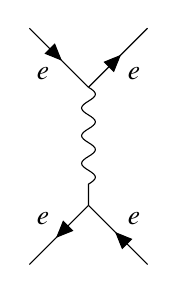
\begin{tikzpicture}[scale=.75]
    \coordinate (A) at (0,4);
    \coordinate (B) at (2,4);
    \coordinate (C) at (1,3);
    \coordinate (D) at (1,1);
    \coordinate (E) at (0,0);
    \coordinate (F) at (2,0);
    \draw[electron] (A) -- node [below left, pos=0.5] {$e$} (C);
    \draw[electron] (C) -- node [below right, pos=0.5] {$e$} (B);
    \draw[photon] (C) -- (D);
    \draw[electron] (F) -- node [above right, pos=0.5] {$e$} (D);
    \draw[electron] (D) -- node [above left, pos=0.5] {$e$} (E);
  \end{tikzpicture}
\end{center}
\noindent This lets us reason with them pictorially.  We can warp a picture without changing the operator it stands for: all that matters is the topology, not the geometry.  In the 1970s, Penrose realized that generalizations of Feynman diagrams arise throughout quantum theory, and might even lead to revisions in our understanding of spacetime 
\cite{Penrose}.  In the 1980s, it became clear that underlying these diagrams is a powerful analogy between quantum physics and topology!  
Namely, a linear operator behaves very much like a `cobordism' ---
that is, an $n$-dimensional manifold going between manifolds of one dimension less:

\begin{center}
  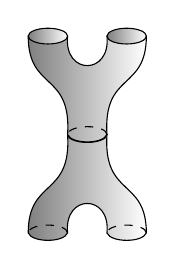
\begin{tikzpicture}[scale=0.5]
    \comultc
    \begin{scope}[yshift=2.5cm]
      \multc
    \end{scope}
  \end{tikzpicture}
\end{center}

\noindent String theory exploits this analogy by replacing the Feynman diagrams of ordinary quantum field theory with 2-dimensional cobordisms, which represent the worldsheets traced out by strings with the passage of time.  The analogy between operators and cobordisms is also important in loop quantum gravity and --- most of all ---
the more purely mathematical discipline of `topological quantum field theory'.  

Meanwhile, quite separately, logicians had begun using categories where the objects represent \emph{propositions} and the morphisms represent \emph{proofs}.  The idea is that a proof is a process going from one proposition (the hypothesis) to another (the conclusion). Later, computer scientists started using categories where the objects represent \emph{data types} and the morphisms represent 
\emph{programs}.   They also started using `flow charts' to describe programs.  Abstractly, these are very much like Feynman diagrams!

The logicians and computer scientists were never very far from each other.  Indeed, the `Curry--Howard correspondence' relating proofs to programs has been well-known at least since the early 1970s, with roots stretching back earlier \cite{Curry,Howard}.  But, it is only in the 1990s that the logicians and computer scientists bumped into the physicists and topologists.  One reason is the rise of interest in quantum cryptography and quantum computation \cite{ChuangNielsen}. With this, people began to think of quantum processes as forms of information processing and to apply ideas from computer science. It was then realized that the loose analogy between flow charts and Feynman diagrams could be made more precise and powerful with the aid of category theory \cite{AC}.

By now there is an extensive network of interlocking analogies between physics, topology, logic and computer science.   They suggest that research in the area of common overlap is actually trying to build a new science: {\it a general science of systems and processes}. Building this science will be very difficult. There are good reasons for this, but also bad ones.  One bad reason is that different fields use different terminology and notation.

The original Rosetta Stone, created in 196 BC, contains versions of the same text in three languages: demotic Egyptian, hieroglyphic script and classical Greek.  Its rediscovery by Napoleon's soldiers let modern Egyptologists decipher the hieroglyphs.  Eventually this led to a vast increase in our understanding of Egyptian culture.

At present, the deductive systems in mathematical logic look like hieroglyphs to most physicists.  Similarly, quantum field theory is Greek to most computer scientists, and so on.  So, there is a need for a new Rosetta Stone to aid researchers attempting to translate between fields. Table \ref{analogy} shows our guess as to what this Rosetta Stone might look like.  

\vskip 1em 
\begin{table}[h]
\begin{center}
%{\baselineskip=18pt
\begin{tabular}{|c|c|c|c|c|}
\hline Category Theory  &  Physics &   Topology  &  Logic       &  Computation \\
\hline object           &  system  &  manifold   &  proposition &  data type \\ 
\hline morphism         &  process &  cobordism  &  proof       &  program  \\
\hline
\end{tabular}
\\
\caption{The Rosetta Stone (pocket version)}
\label{analogy}
%}
\end{center}
\end{table}
The rest of this chapter expands on this table by comparing how categories are used in physics, topology, logic, and computation. Unfortunately, these different fields focus on slightly different kinds of categories.  Though most physicists don't know it, quantum physics has long made use of `compact symmetric monoidal categories'.  Knot theory uses 
`compact braided monoidal categories', which are slightly more general. However, it became clear in the 1990's that these more general gadgets are useful in physics too. Logic and computer science used to focus on `cartesian closed categories' --- 
where `cartesian' can be seen, roughly, as an antonym of `quantum'. However, thanks to work on linear logic and quantum computation, some logicians and computer scientists have dropped their insistence on cartesianness: now they study more general sorts of `closed symmetric monoidal categories'.

In Section \ref{physics_topology} we explain these concepts, how they illuminate the analogy between physics and topology, and how to work with them using string diagrams.  We assume no prior knowledge of category theory, only a willingness to learn some. In Section \ref{logic} we explain how closed symmetric monoidal categories correspond to a small fragment of ordinary propositional logic, which also happens to be a fragment of Girard's 
`linear logic' \cite{Girard1}.   In Section \ref{computation} 
we explain how closed symmetric monoidal categories correspond to a simple model of computation.   Each of these sections starts with some background material.  In Section \ref{conclusions}, we conclude by presenting a larger version of the Rosetta Stone.

Our treatment of all four subjects --- physics, topology, logic and computation --- is bound to seem sketchy, narrowly focused and idiosyncratic to practitioners of these subjects.  Our excuse is that we wish to emphasize certain analogies while saying no more than absolutely necessary.  To make up for this, we include many references for those who wish to dig deeper.

\section{The Analogy Between Physics and Topology}
\label{physics_topology}

\subsection{Background}
\label{ptbackground}

Currently our best theories of physics are general relativity and the Standard Model of particle physics.  The first describes gravity without taking quantum theory into account; the second describes all the other forces taking quantum theory into account, but ignores gravity.  So, our world-view is deeply schizophrenic. The field where physicists struggle to solve this problem is called {\em quantum gravity}, since it is widely believed that the solution requires treating gravity in a way that takes quantum theory into account.

\begin{table}[h]
\begin{center}
\begin{tabular}{|c|c|}                    \hline Physics                           &  Topology \\  \hline Hilbert space                     &  $(n-1)$-dimensional manifold       \\  
(system)                          & (space)             \\  \hline operator between                  &  cobordism between  \\
Hilbert spaces                    & $(n-1)$-dimensional manifolds \\
(process)                         &  (spacetime)           \\  \hline composition of operators          &  composition of cobordisms \\  \hline identity operator                 &  identity cobordism \\  \hline
\end{tabular} 
\\
\caption{Analogy between physics and topology}
\label{analogy2}
\end{center}
\end{table}

Nobody is sure how to do this, but there is a striking similarity between two of the main approaches: string theory and loop quantum gravity.  Both rely on the analogy between physics and topology shown in Table \ref{analogy2}. On the left we have a basic ingredient of quantum theory: 
the category $\Hilb$ whose objects are Hilbert spaces, used to describe physical {\em systems}, and whose morphisms are linear operators, used to describe physical {\em processes}.  On the right we have a basic structure in differential topology: the category $n\Cob$. Here the objects are $(n-1)$-dimensional manifolds, used to describe
{\em space}, and whose morphisms are $n$-dimensional cobordisms, used to describe {\em spacetime}.  

As we shall see, $\Hilb$ and $n\Cob$ share many structural features. Moreover, both are very different from the more familiar category $\Set$, whose objects are sets and whose morphisms are functions. Elsewhere we have argued at great length that this is important for better understanding quantum gravity \cite{B3} and even the foundations of quantum theory \cite{B4}.  The idea is that if $\Hilb$ is more like 
$n\Cob$ than $\Set$, maybe we should stop thinking of a quantum process as a function from one set of states to another.  Instead, maybe we should think of it as resembling a `spacetime' going between spaces of dimension one less.   

This idea sounds strange, but the simplest example is something very practical, used by physicists every day: a Feynman diagram.  This is a 1-dimensional graph going between 0-dimensional collections of points, with edges and vertices labelled in certain ways.  Feynman diagrams are topological entities, but they describe linear operators. String theory uses 2-dimensional cobordisms equipped with extra structure --- string worldsheets --- to do a similar job.  Loop quantum gravity uses 2d generalizations of Feynman diagrams called `spin foams' \cite{B2}.  Topological quantum field theory uses higher-dimensional cobordisms \cite{HDATQFT}.  In each case, processes are described by morphisms in a special sort of category: a `compact symmetric monoidal category'.

In what follows, we shall not dwell on puzzles from quantum theory or quantum gravity.  Instead we take a different tack, simply explaining some basic concepts from category theory and showing how $\Set$, 
$\Hilb$, $n\Cob$ and categories of tangles give examples.  A recurring theme, however, is that $\Set$ is very different from the other examples.

To help the reader safely navigate the sea of jargon, here is a chart of the concepts we shall explain in this section:
\[
\xymatrix{
*+[F]\txt{categories}\ar@{-}[d] 
\\
*+[F]\txt{monoidal categories}\ar@{-}[d] \ar@{-}[dr] 
\\
*+[F]\txt{braided \\ monoidal categories}\ar@{-}[d] \ar@{-}[dr] 
&*+[F]\txt{closed \\ monoidal categories}\ar@{-}[d] \ar@{-}[dr]
\\
*+[F]\txt{symmetric \\ monoidal categories} \ar@{-}[d] \ar@{-}[dr] 
&*+[F]\txt{closed braided \\ monoidal categories}\ar@{-}[d] \ar@{-}[dr] 
&*+[F]\txt{compact \\ monoidal categories}\ar@{-}[d] 
\\
*+[F]\txt{cartesian categories} \ar@{-}[d] 
&*+[F]\txt{closed symmetric \\ monoidal categories}\ar@{-}[dl] \ar@{-}[dr] 
&*+[F]\txt{compact braided \\ monoidal categories}\ar@{-}[d] 
\\
*+[F]\txt{cartesian \\ closed categories} 
& & *+[F]\txt{compact symmetric \\ monoidal categories} 
} 
\]

\vskip 1em
\noindent The category $\Set$ is cartesian closed, while $\Hilb$ and $n\Cob$ are compact symmetric monoidal.

\subsection{Categories}
\label{categories}

Category theory was born around 1945, with Eilenberg and Mac Lane
\cite{EM} defining `categories', `functors' between categories, and `natural transformations' between functors.  By now there are many introductions to the subject
\cite{Crole,MacLane2,McLarty}, including some available for free online \cite{JLBell,Goldblatt}.  Nonetheless, we begin at the beginning:

\begin{definition} A {\bf category} $C$ consists of:
\begin{itemize}
    \item a collection of {\bf objects}, where if $X$ is an object of $C$
    we write $X \in C$, and
    \item for every pair of objects $(X,Y),$ a set $\hom(X,Y)$ of 
    {\bf morphisms} from $X$ to $Y$.  We call this set $\hom(X,Y)$ a
    {\bf homset}.  If $f \in \hom(X,Y),$ then we write $f\maps X\to Y.$
\end{itemize}
such that:
\begin{itemize}
    \item for every object $X$ there is an {\bf identity morphism} $1_X\maps 
     X\to X;$
    \item morphisms are composable: given $f\maps X\to Y$ and $g\maps
    Y\to Z,$ there is a {\bf composite morphism} $gf \maps X \to Z;$
    sometimes also written $g \circ f$.
    \item an identity morphism is both a {\bf left and a right unit} for 
   composition: if $f \maps X\to Y,$ then $f 1_X = f = 1_Y f;$ and
    \item composition is {\bf associative}: $(h g) f = 
   h (g f)$ whenever either side is well-defined.
\end{itemize}
\end{definition}

\begin{definition}
  We say a morphism $f\maps X \to Y$ is an \textbf{isomorphism} if it
  has an inverse--- that is, there exists another morphism $g\maps Y
  \to X$ such that $gf = 1_X$ and $fg = 1_Y.$
\end{definition}

A category is the simplest framework where we can talk about systems (objects) and processes (morphisms).  To visualize these, we can use `Feynman diagrams' of a very primitive sort.  In applications to linear algebra, these diagrams are often called `spin networks', but category theorists call them `string diagrams', and that is the term we will use.  The term `string' here has little to do with string theory: 
instead, the idea is that objects of our category label `strings' or `wires':
\[\begin{pspicture}(0,0)(1,2)
\psset{angleA=-90,angleB=90,ArrowInside=->,arrowscale=2}
\pnode(0,2){A}
\pnode(1,0){B}
\nccurve{A}{B} \nbput{$X$}
\end{pspicture}\]
and morphisms $f \maps X \to Y$ label `black boxes' with an input wire of type $X$ and an output wire of type $Y$:
\[\begin{pspicture}(0,0)(2,4)
\psset{angleA=-90,angleB=90,ArrowInside=->,arrowscale=2}
\pnode(1,4){A}
\rput(1,2){\ovalnode{B}{$f$}}
\pnode(1,0){C}
\nccurve{A}{B} \nbput{$X$}
\nccurve{B}{C} \nbput{$Y$}
\end{pspicture}\]
We compose two morphisms by connecting the output of one black box to the input of the next.  So, the composite of $f\maps X \to Y$
and $g\maps Y \to Z$ looks like this:
\begin{center}
    \begin{pspicture}(0,0)(2,6)
    \psset{angleA=-90,angleB=90,ArrowInside=->,arrowscale=2}
    \pnode(1,6){A}
    \rput(1,4){\ovalnode{B2}{$f$}}
    \rput(1,2){\ovalnode{B1}{$g$}}
    \pnode(1,0){C}
    \nccurve{A}{B2} \nbput{$X$}
    \nccurve{B2}{B1} \nbput{$Y$}
    \nccurve{B1}{C} \nbput{$Z$}
    \end{pspicture}
\end{center}
Associativity of composition is then implicit:
\begin{center}
    \begin{pspicture}(0,0)(2,8)
    \psset{angleA=-90,angleB=90,ArrowInside=->,arrowscale=2}
    \pnode(1,8){A}
    \rput(1,6){\ovalnode{B3}{$f$}}
    \rput(1,4){\ovalnode{B2}{$g$}}
    \rput(1,2){\ovalnode{B1}{$h$}}
    \pnode(1,0){C}
    \nccurve{A}{B3} \nbput{$X$}
    \nccurve{B3}{B2} \nbput{$Y$}
    \nccurve{B2}{B1} \nbput{$Z$}
    \nccurve{B1}{C} \nbput{$W$}
    \end{pspicture}
\end{center}
is our notation for both $h (g f)$ and 
$(h g) f$.  Similarly, if we draw the identity morphism $1_X \maps X \to X$ as a piece of wire of type $X$:
\[\begin{pspicture}(0,0)(1,2)
\psset{angleA=-90,angleB=90,ArrowInside=->,arrowscale=2}
\pnode(1,2){A}
\pnode(1,0){B}
\nccurve{A}{B} \nbput{$X$}
\end{pspicture}\]
then the left and right unit laws are also implicit.

There are countless examples of categories, but we will focus on four:
\begin{itemize}
\item $\Set$: the category where objects are sets.
\item $\Hilb$: the category where objects are finite-dimensional 
      Hilbert spaces.
\item $n\Cob$: the category where morphisms are $n$-dimensional 
      cobordisms.
\item $\Tang_k$: the category where morphisms are $k$-codimensional
      tangles.
\end{itemize}
As we shall see, all four are closed symmetric monoidal categories, at least when $k$ is big enough.  However, the most familiar of the lot, namely $\Set$, is the odd man out: it is `cartesian'.

Traditionally, mathematics has been founded on the category $\Set$, where the objects are {\em sets} and the morphisms are {\em functions}.  So, when we study systems and processes in physics, it is tempting to specify a system by giving its set of states, and a process by giving a function from states of one system to states of another.

However, in quantum physics we do something subtly different:
we use categories where objects are {\em Hilbert spaces} 
and morphisms are {\em bounded linear operators}.  We specify a system by giving a Hilbert space, but this Hilbert space is not really the set of states of the system: a state is actually a ray in Hilbert space.  Similarly, a bounded linear operator is not precisely a function from states of one system to states of another.  

In the day-to-day practice of quantum physics, what really matters is not sets of states and functions between them, but Hilbert space and operators.  One of the virtues of category theory is that it frees us from the `$\Set$-centric' view of traditional mathematics and lets us view quantum physics on its own terms.  As we shall see, this sheds new light on the quandaries that have always plagued our understanding of the quantum realm \cite{B4}.

To avoid technical issues that would take us far afield, we will take $\Hilb$ to be the category where objects are {\em finite-dimensional Hilbert spaces} and morphisms are {\em linear operators}
(automatically bounded in this case).  Finite-dimensional Hilbert spaces suffice for some purposes; infinite-dimensional ones are often important, but treating them correctly would require some significant extensions of the ideas we want to explain here.

In physics we also use categories where the objects represent choices of {\em space}, and the morphisms represent choices of {\em spacetime}.  The simplest is $n\Cob$, where the objects are {\em
$(n-1)$-dimensional manifolds}, and the morphisms are {\em
$n$-dimensional cobordisms}.  Glossing over some subtleties that a careful treatment would discuss \cite{Sawin}, a cobordism 
$f \maps X \to Y$ is an $n$-dimensional manifold whose boundary is the disjoint union of the $(n-1)$-dimensional manifolds $X$ and $Y$. Here are a couple of cobordisms in the case $n = 2$:
\begin{center}
  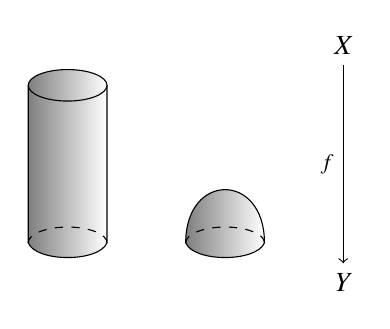
\begin{tikzpicture}
    \medidentc
    \begin{scope}[xshift=2cm]
      \birthc
    \end{scope}
    \node (Y) at (3.5, -.5) {$Y$};
    \node (X) at (3.5, 2.5) {$X$}
      edge [->] node [left, l] {$f$} (Y);
  \end{tikzpicture}
  $\qquad \qquad$
  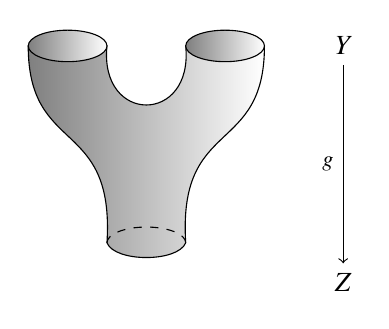
\begin{tikzpicture}
    \begin{scope}[xshift=1cm]
      \multc
    \end{scope}
    \node (Z) at (3.5, -.5) {$Z$};
    \node (Y) at (3.5, 2.5) {$Y$}
      edge [->] node [left, l] {$g$} (Z);
  \end{tikzpicture}
\end{center}
We compose them by gluing the `output' of one to the `input' of the other.   So, in the above example $gf \maps X \to Z$ looks like this:
\begin{center}
  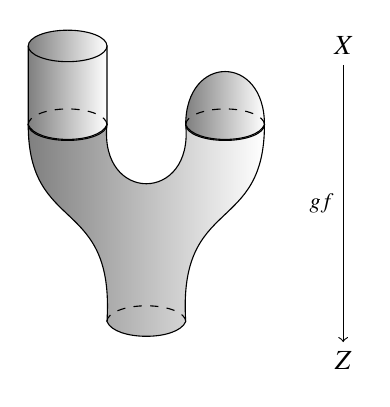
\begin{tikzpicture}
    \multc
    \begin{scope}[xshift=-1cm, yshift=2.5cm]
      \smallidentc
    \end{scope}
    \begin{scope}[xshift=1cm, yshift=2.5cm]
      \birthc
    \end{scope}
    \node (Z) at (2.5, -.5) {$Z$};
    \node (X) at (2.5, 3.5) {$X$}
      edge [->] node [left, l] {$gf$} (Z);
  \end{tikzpicture}
\end{center}

Another kind of category important in physics has objects representing
{\em collections of particles}, and morphisms representing their {\em worldlines and interactions}.  Feynman diagrams are the classic example, but in these diagrams the `edges' are not taken literally as particle trajectories.  An example with closer ties to topology is
$\Tang_k$.  

Very roughly speaking, an object in $\Tang_k$ is a collection of points in a $k$-dimensional cube, while a morphism is a `tangle':
a collection of arcs and circles smoothly embedded in a 
$(k+1)$-dimensional cube, such that the circles lie in the interior of the cube, while the arcs touch the boundary of the cube only at its top and bottom, and only at their endpoints.  A bit more precisely, tangles are `isotopy classes' of such embedded arcs and circles: this equivalence relation means that only the topology of the tangle matters, not its geometry.  We compose tangles by attaching one cube to another top to bottom.

More precise definitions can be found in many sources, at least for
$k = 2$, which gives tangles in a 3-dimensional cube \cite{FY, Kassel,Sawin,Shum,Turaev,Yetter}.  But since a picture is worth a thousand words, here is a picture of a morphism in $\Tang_2$:
\[  
\epsfysize=1.5in\epsfbox{3dtangle.eps}
\quad
 \xy
 {\ar_{f} (0,38)*+{X}; (0,0)*+{Y}};
 \endxy
\]
\noindent Note that we can think of a morphism in $\Tang_k$ as a 1-dimensional cobordism {\it embedded in a $k$-dimensional cube}.  This is why 
$\Tang_k$ and $n\Cob$ behave similarly in some respects.

Here are two composable morphisms in $\Tang_1$:
\[
\text{\epsfysize=1.2in\epsfbox{2dtangle.eps}} 
\quad
 \xy
 {\ar_{f} (0,30)*+{X}; (0,0)*+{Y}};
 \endxy
\qquad \qquad
\text{\epsfysize=1.2in\epsfbox{another2dtangle.eps}}
\quad
 \xy
 {\ar_{g} (0,30)*+{Y}; (0,0)*+{Z}};
 \endxy
\]
and here is their composite:
\[  
\epsfysize=2.2in\epsfbox{compositetangle.eps}
\quad
 \xy
 {\ar_{gf} (0,55)*+{X}; (0,0)*+{Z}};
 \endxy
\]
Since only the tangle's topology matters, we are free to squash this rectangle into a square if we want, but we do not need to.

It is often useful to consider tangles that are decorated in various ways.  For example, in an `oriented' tangle, each arc and circle is equipped with an orientation.  We can indicate this by drawing a little arrow on each curve in the tangle.  In applications to physics, these curves represent worldlines of particles, and the arrows say whether each particle is going forwards or backwards in time, following Feynman's idea that antiparticles are particles going backwards in time. We can also consider `framed' tangles.  Here each curve is replaced by a `ribbon'.  In applications to physics, this keeps track of how each particle twists.  This is especially important for fermions, where a 
$2\pi$ twist acts nontrivially.  Mathematically, the best-behaved tangles are both framed and oriented \cite{HDATQFT,Shum}, and these are what we should use to define $\Tang_k$.  The category $n\Cob$ also has a framed oriented version.  However, these details will barely matter in what is to come.

It is difficult to do much with categories without discussing the maps between them.  A map between categories is called a `functor':

\begin{definition} 
A {\bf functor} $F\maps C\to D$ from a category $C$ to a category $D$
is a map sending:
\begin{itemize}
\item any object $X \in C$ to an object $F(X) \in D$,
\item any morphism $f\maps X\to Y$ in $C$ to a morphism $F(f)\maps F(X)\to F(Y)$ 
in $D$,
\end{itemize}
in such a way that:
\begin{itemize}
\item $F$ {\bf preserves identities}: for any object $X \in C$,
$F(1_X) = 1_{F(X)}$;
\item $F$ {\bf preserves composition}: for any pair of morphisms $f \maps X \to Y$, $g \maps Y \to Z$ in $C$,
$F(gf) = F(g) F(f)$.
\end{itemize}
\end{definition}

In the sections to come, we will see that functors and natural transformations are useful for putting extra structure on categories. Here is a rather different use for functors: we can think of a functor $F \maps C \to D$ as giving a picture, or `representation', of $C$ in $D$.  The idea is that $F$ can map objects and morphisms of some `abstract' category $C$ to objects and morphisms of a more `concrete' category $D$.  

For example, consider an abstract group $G$.  This is the same as a category with one object and with all morphisms invertible. The object is uninteresting, so we can just call it $\bullet$, but the morphisms are the elements of $G$, and we compose them by multiplying them.  From this perspective, a {\bf representation} of $G$ on a finite-dimensional Hilbert space is the same as a functor 
$F \maps G \to \Hilb$.  Similarly, an {\bf action} of $G$ 
on a set is the same as a functor $F \maps G \to \Set$.  Both notions are ways of making an abstract group more concrete.

Ever since Lawvere's 1963 thesis on functorial semantics
\cite{Lawvere}, the idea of functors as representations has become pervasive.  However, the terminology varies from field to field. Following Lawvere, logicians often call the category $C$ a `theory', and call the functor $F \maps C \to D$ a `model' of this theory. Other mathematicians might call $F$ an `algebra' of the theory. In this work, the default choice of $D$ is usually the category
$\Set$.  

In physics, it is the functor $F \maps C \to D$ that is called the `theory'.  Here the default choice of $D$ is either the category we are calling $\Hilb$ or a similar category of \emph{infinite-dimensional}
Hilbert spaces.  For example, both `conformal field theories' \cite{Segal} 
and topological quantum field theories \cite{AtiyahTQFT} can be seen as functors of this sort.

If we think of functors as models, natural transformations are maps between models:

\begin{definition} 
\label{naturality}
Given two functors $F,F'\maps C\to D,$ a {\bf natural transformation} $\alpha\maps F \Rightarrow F'$ assigns to every object
$X$ in $C$ a morphism $\alpha_X\maps F(X)\to F'(X)$ such that for any morphism $f\maps X \to Y$ in $C,$ the equation $\alpha_Y \, F(f) = F'(f)
\, \alpha_X$ holds in $D.$   In other words, this square commutes:
\[\begin{diagram}
\node{F(X)}\arrow{e,t}{F(f)}\arrow{s,l}{\alpha_X}\node{F(Y)}
\arrow{s,r}{\alpha_Y}\\
\node{F'(X)}\arrow{e,b}{F'(f)}\node{F'(Y)}
\end{diagram}\]
(Going across and then down equals going down and then across.)
\end{definition}

\begin{definition} A {\bf natural isomorphism} between functors
$F,F' \maps C \to D$ is a natural transformation $\alpha \maps F
\Rightarrow F'$ such that $\alpha_X$ is an isomorphism for every $X \in C$.
\end{definition}

For example, suppose $F, F' \maps G \to \Hilb$ are functors where
$G$ is a group, thought of as a category with one object, say $\bullet$. Then, as already mentioned, $F$ and $F'$ are secretly just representations of $G$ on the Hilbert spaces $F(\bullet)$ and $F'(\bullet)$.  A natural transformation $\alpha \maps F \To F'$ is then the same as an {\bf intertwining operator} from one representation to another: that is, a linear operator 
\[  A \maps F(\bullet) \to F'(\bullet) \]
satisfying
\[  A F(g) = F'(g) A \]
for all group elements $g$. 

\subsection{Monoidal Categories}
\label{monoidal}

In physics, it is often useful to think of two systems sitting side by side as forming a single system.  In topology, the disjoint union of two manifolds is again a manifold in its own right.  In logic, the conjunction of two statement is again a statement.  In programming we can combine two data types into a single `product type'. The concept of `monoidal category' unifies all these examples in a single framework.

A monoidal category $C$ has a functor $\tensor \maps C \times C \to C$
that takes two objects $X$ and $Y$ and puts them together to give a new object $X \tensor Y$.  To make this precise, we need the cartesian product of categories:

\begin{definition} The {\bf cartesian product} $C \times C'$ of categories $C$ and $C'$ is the category where:
\begin{itemize}
\item an object is a pair $(X,X')$ consisting of an object $X \in C$ and an object 
$X' \in C'$;
\item a morphism from $(X,X')$ to $(Y,Y')$ is a pair $(f,f')$ consisting of a morphism $f \maps X \to Y$ and a morphism $f' \maps X' \to Y'$;
\item composition is done componentwise: $(g,g')(f,f') = (gf,g'f')$;
\item identity morphisms are defined componentwise:
$1_{(X,X')} = (1_X, 1_{X'})$.
\end{itemize}
\end{definition}

Mac Lane \cite{MacLane} defined monoidal categories in 1963.  The subtlety of the definition lies in the fact that $(X \tensor Y)
\tensor Z$ and $X \tensor (Y \tensor Z)$ are not usually equal. Instead, we should specify an isomorphism between them, called the
`associator'.  Similarly, while a monoidal category has a `unit object' $I$, it is not usually true that $I \tensor X$ and $X \tensor I$ 
equal $X$.  Instead, we should specify isomorphisms $I \tensor X \cong X$
and $X \tensor I \cong X$.  To be manageable, all these isomorphisms must then satisfy certain equations:

\begin{definition}
\label{mon.cat}
A {\bf monoidal category} consists of:
    \begin{itemize}
        \item a category $C,$
        \item a {\bf tensor product} functor $\tensor \maps
       C\times C\to C,$ 
        \item a {\bf unit object} $I \in C$,
        \item a natural isomorphism called the {\bf associator}, assigning to each triple of objects $X,Y,Z \in C$ an isomorphism
        \[a_{X,Y,Z}:(X \tensor Y)\tensor Z \isoto X \tensor (Y \tensor Z),\]
        \item natural isomorphisms called the {\bf left} and {\bf right unitors}, assigning to each object $X \in C$ isomorphisms 
        \[l_X:I\tensor X \isoto X\]
        \[r_X:X\tensor I \isoto X,\]
    \end{itemize}
    such that:
    \begin{itemize}
        \item for all $X,Y \in C$ the {\bf triangle equation} holds:
        \di{
            \node{(X\tensor I)\tensor Y}\arrow[2]{e,t}{a_{X,I,Y}}\arrow{se,b}{r_X\tensor 1_Y}\node[2]{X\tensor(I\tensor Y)}\arrow{sw,b}{1_X\tensor l_Y}\\
            \node[2]{X\tensor Y}
        }
        \item for all $W,X,Y,Z \in C$, the {\bf pentagon equation} holds:
        \di{
            \node[2]{((W\tensor X)\tensor Y)\tensor Z}\arrow{ssw,t}{a_{W\tensor X,Y,Z}}\arrow{se,t}{a_{W,X,Y}\tensor 1_Z}\\
            \node[3]{(W\tensor (X\tensor Y))\tensor Z}\arrow[2]{s,r}{a_{W,X\tensor Y,Z}}\\
            \node{(W\tensor X)\tensor(Y\tensor Z)}\arrow{sse,b}{a_{W,X,Y\tensor Z}}\\
            \node[3]{W\tensor ((X\tensor Y)\tensor Z)}\arrow{sw,r}{1_W\tensor a_{X,Y,Z}}\\
            \node[2]{W\tensor(X\tensor(Y\tensor Z))}
        }
    \end{itemize}
\end{definition}

When we have a tensor product of four objects, there are five ways to parenthesize it, and at first glance the associator lets us build two isomorphisms from $W \tensor (X \tensor (Y \tensor Z))$ to
$((W \tensor X) \tensor Y) \tensor Z$.  But, the pentagon equation says these isomorphisms are equal.  When we have tensor products of even more objects there are even more ways to parenthesize them, and even more isomorphisms between them built from the associator. However, Mac Lane showed that the pentagon identity implies these isomorphisms are all the same.  Similarly, if we also assume the triangle equation, all isomorphisms with the same source and target built from the associator, left and right unit laws are equal.

In a monoidal category we can do processes in `parallel' as well as in `series'.  Doing processes in series is just composition of morphisms, which works in any category.  But in a monoidal category we can also tensor morphisms $f \maps X \to Y$ and $f' \maps X' \to Y'$ and obtain a `parallel process' $f \tensor f' \maps X \tensor X' \to Y \tensor Y'$.  We can draw this in various ways:

\[\begin{pspicture}(0,0)(15,4)
\psset{angleA=-90,angleB=90,ArrowInside=->,arrowscale=2}
\pnode(1,4){A}
\rput(1,2){\ovalnode{B}{$f$}}
\pnode(1,0){C}
\nccurve{A}{B} \nbput{$X$}
\nccurve{B}{C} \nbput{$Y$}

\pnode(3,4){A}
\rput(3,2){\ovalnode{B}{$f'$}}
\pnode(3,0){C}
\nccurve{A}{B} \nbput{$X'$}
\nccurve{B}{C} \nbput{$Y'$}

\rput(5,2){=}

\pnode(7,4){A}
\pnode(9,4){A2}
\rput(8,2){\ovalnode{B}{$f \tensor f'$}}
\pnode(7,0){C}
\pnode(9,0){C2}
\nccurve[angleB=135]{A}{B} \nbput{$X$}
\nccurve[angleA=-135]{B}{C} \nbput{$Y$}
\nccurve[angleB=45]{A2}{B} \naput{$X'$}
\nccurve[angleA=-45]{B}{C2} \naput{$Y'$}

\rput(11,2){=}

\pnode(13,4){A}
\rput(13,2){\ovalnode{B}{$f \tensor f'$}}
\pnode(13,0){C}
\nccurve{A}{B} \nbput{$X \tensor X'$}
\nccurve{B}{C} \nbput{$Y \tensor Y'$}

\end{pspicture}\]

More generally, we can draw any morphism 
\[f \maps X_1 \tensor \cdots \tensor X_n \to 
          Y_1 \tensor \cdots \tensor Y_m \]
as a black box with $n$ input wires and $m$ output wires:
\[\begin{pspicture}(0,0)(4,4)
\psset{angleA=-90,angleB=90,ArrowInside=->,arrowscale=2}
    \pnode(0,4){X1}
    \pnode(2,4){X2}
    \pnode(4,4){X3}
    \rput(2,2){\ovalnode{F}{$f$}}
    \pnode(1,0){Y1}
    \pnode(3,0){Y2}
    \nccurve[angleB=135]{X1}{F} \nbput[npos=0]{$X_1$}
    \nccurve{X2}{F} \nbput[npos=0]{$X_2$}
    \nccurve[angleB=45]{X3}{F} \naput[npos=0]{$X_3$}
    \nccurve[angleA=-120]{F}{Y1} \nbput[npos=1]{$Y_1$}
    \nccurve[angleA=-60]{F}{Y2} \naput[npos=1]{$Y_2$}
\end{pspicture}\]
We draw the unit object $I$ as a blank space.  So, for example, we draw a morphism $f \maps I \to X$ as follows:
\[\begin{pspicture}(0,0)(2,3)
\psset{angleA=-90,angleB=90,ArrowInside=->,arrowscale=2}
\pnode(1,3){A}
\rput(1,2){\ovalnode{B}{$f$}}
\pnode(1,0){C}
\nccurve{B}{C} \nbput{$X$}
\end{pspicture}\]
By composing and tensoring morphisms, we can build up elaborate pictures resembling Feynman diagrams:
\[\begin{pspicture}(0,0)(8,6)
  \psset{angleA=-90,angleB=90,ArrowInside=->,arrowscale=2}
  \pnode(1,6){X1}
  \pnode(2,6){X2}
  \pnode(5,6){X3}
  \pnode(7,6){X4}
  \rput(1,2){\ovalnode{F}{$f$}}
  \rput(2,1){\ovalnode{G}{$g$}}
  \rput(5,2.5){\ovalnode{H}{$h$}}
  \rput(7,4){\ovalnode{J}{$j$}}
  \pnode(1,0){Y1}
  \pnode(2,0){Y2}
  \pnode(5,0){Y3}
  \pnode(7,0){Y4}
  \nccurve{X1}{F} \nbput[npos=0]{$X_1$}
  \nccurve[angleB=60]{X2}{G} \naput[npos=0]{$X_2$}
  \nccurve{X3}{H} \nbput[npos=0]{$X_3$}
  \nccurve{X4}{J} \nbput[npos=0]{$X_4$}
  \nccurve[angleA=-120]{F}{Y1} \nbput[npos=1]{$Y_1$}
  \nccurve{G}{Y2} \naput[npos=1]{$Y_2$}
  \nccurve{H}{Y3} \nbput[npos=1]{$Y_3$}
  \nccurve{J}{Y4} \nbput[npos=1]{$Y_4$}
  \nccurve[angleA=-60, angleB=120]{F}{G} \naput{$Z$}
\end{pspicture}\]
The laws governing a monoidal category allow us to neglect associators and unitors when drawing such pictures, without getting in trouble.  The reason is that Mac Lane's Coherence Theorem says any monoidal category is `equivalent', in a suitable sense, to one where all associators and unitors are identity morphisms \cite{MacLane}.

We can also deform the picture in a wide variety of ways without changing the morphism it describes. For example, the above morphism equals this one:
\[\begin{pspicture}(0,0)(8,6)
    \psset{angleA=-90,angleB=90,ArrowInside=->,arrowscale=2}
    \pnode(1,6){X1}
    \pnode(2,6){X2}
    \pnode(5,6){X3}
    \pnode(7,6){X4}
    \rput(1,5){\ovalnode{F}{$f$}}
    \rput(2,3){\ovalnode{G}{$g$}}
    \rput(4,4){\ovalnode{H}{$h$}}
    \rput(6.5,2){\ovalnode{J}{$j$}}
    \pnode(1,0){Y1}
    \pnode(2,0){Y2}
    \pnode(5,0){Y3}
    \pnode(7,0){Y4}
    \nccurve[ArrowInsidePos=.75]{X1}{F} \nbput[npos=0]{$X_1$}
    \nccurve[angleB=60]{X2}{G} \naput[npos=0]{$X_2$}
    \nccurve{X3}{H} \nbput[npos=0]{$X_3$}
    \nccurve{X4}{J} \nbput[npos=0]{$X_4$}
    \nccurve[angleA=-120]{F}{Y1} \nbput[npos=1]{$Y_1$}
    \nccurve{G}{Y2} \naput[npos=1]{$Y_2$}
    \nccurve{H}{Y3} \nbput[npos=1]{$Y_3$}
    \nccurve{J}{Y4} \naput[npos=1]{$Y_4$}
    \nccurve[angleA=-60, angleB=120]{F}{G} \nbput{$Z$}
\end{pspicture}\]
Everyone who uses string diagrams for calculations in monoidal categories starts by worrying about the rules of the game:
{\em precisely how} can we deform these pictures without changing the morphisms they describe?  Instead of stating the rules precisely
--- which gets a bit technical --- we urge you to explore for yourself what is allowed and what is not.  For example, show that we can slide black boxes up and down like this:
\[\begin{pspicture}(0,0)(3,3)
    \psset{angleA=-90,angleB=90,ArrowInside=->,arrowscale=2}
    \pnode(1,3){X1}
    \pnode(2,3){X2}
    \rput(1,2){\ovalnode{F}{$f$}}
    \rput(2,1){\ovalnode{G}{$g$}}
    \pnode(1,0){Y1}
    \pnode(2,0){Y2}
    \nccurve{X1}{F} \nbput[npos=0]{$X_1$}
    \nccurve{F}{Y1} \nbput[npos=1]{$Y_1$}
    \nccurve{X2}{G} \naput[npos=0]{$X_2$}
    \nccurve{G}{Y2} \naput[npos=1]{$Y_2$}
\end{pspicture} \begin{pspicture}(0,0)(2,3)
    \rput(1,1.5){=}
\end{pspicture} \begin{pspicture}(0,0)(3,3)
    \psset{angleA=-90,angleB=90,ArrowInside=->,arrowscale=2}
    \pnode(1,3){X1}
    \pnode(2,3){X2}
    \rput(1,1.5){\ovalnode{F}{$f$}}
    \rput(2,1.5){\ovalnode{G}{$g$}}
    \pnode(1,0){Y1}
    \pnode(2,0){Y2}
    \nccurve{X1}{F} \nbput[npos=0]{$X_1$}
    \nccurve{F}{Y1} \nbput[npos=1]{$Y_1$}
    \nccurve{X2}{G} \naput[npos=0]{$X_2$}
    \nccurve{G}{Y2} \naput[npos=1]{$Y_2$}
\end{pspicture} \begin{pspicture}(0,0)(2,3)
    \rput(1,1.5){=}
\end{pspicture} \begin{pspicture}(0,0)(3,3)
    \psset{angleA=-90,angleB=90,ArrowInside=->,arrowscale=2}
    \pnode(1,3){X1}
    \pnode(2,3){X2}
    \rput(1,1){\ovalnode{F}{$f$}}
    \rput(2,2){\ovalnode{G}{$g$}}
    \pnode(1,0){Y1}
    \pnode(2,0){Y2}
    \nccurve{X1}{F} \nbput[npos=0]{$X_1$}
    \nccurve{F}{Y1} \nbput[npos=1]{$Y_1$}
    \nccurve{X2}{G} \naput[npos=0]{$X_2$}
    \nccurve{G}{Y2} \naput[npos=1]{$Y_2$}
\end{pspicture}\]
For a formal treatment of the rules governing string diagrams, try the original papers by Joyal and Street \cite{JS0}
and the book by Yetter \cite{Yetter}.

Now let us turn to examples.  Here it is crucial to realize that the same category can often be equipped with different tensor products, resulting in different monoidal categories:

\begin{itemize}

\item There is a way to make $\Set$ into a monoidal category where
$X \tensor Y$ is the cartesian product $X \times Y$ and the unit object is any one-element set.  Note that this tensor product is not strictly associative, since $(x, (y, z)) \ne ((x, y), z),$ but there's a natural isomorphism $(X \times Y) \times Z \iso X \times (Y \times Z)$, and this is our associator.  Similar considerations give the left and right unitors.  In this monoidal category, the tensor product of $f \maps X \to Y$ and $f' \maps X' \to Y'$ is the function
\[
\begin{array}{rccl}
        f \times f' & \maps X\times X'& \to& Y\times Y' \\
                    & (x,x') &\mapsto & (f(x),f'(x')) .
\end{array}
\]

There is also a way to make $\Set$ into a monoidal category where
$X \tensor Y$ is the disjoint union of $X$ and $Y$, which we shall denote by $X + Y$.  Here the unit object is the empty set. Again, as indeed with all these examples, the associative law and left/right unit laws hold only up to natural isomorphism.  In this monoidal category, the tensor product of $f \maps X \to Y$ and 
$f' \maps X' \to Y'$ is the function
\[
\begin{array}{rccl}
 f+f' \maps & X+X'  &\to&  Y+Y'  \\
           &      x &\mapsto& 
\left\{
\begin{array}{cl} 
f(x) & \text{if $x \in X$,} \\ 
f'(x) & \text{if $x \in X'$.}
\end{array} \right.
\end{array}
\]

{\em However, in what follows, when we speak of $\Set$ as a monoidal category, we always use the cartesian product!}

\item There is a way to make $\Hilb$ into a monoidal category with the usual tensor product of Hilbert spaces: $\CC^n \tensor \CC^m \cong 
\CC^{nm}.$  In this case the unit object $I$ can be taken to be a
1-dimensional Hilbert space, for example $\CC$.  

There is also a way to make $\Hilb$ into a monoidal category where the tensor product is the direct sum: $\CC^n \oplus \CC^m \cong 
\CC^{n+m}.$  In this case the unit object is the zero-dimensional Hilbert space, $\{ 0\}.$

{\em However, in what follows, when we speak of $\Hilb$ as a monoidal category, we always use the usual tensor product!}

\item The tensor product of objects and morphisms in $n\Cob$ is given by disjoint union.  For example, the tensor product of these two morphisms:
\begin{center}
  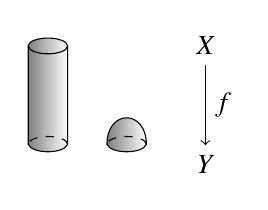
\begin{tikzpicture}[scale=.5]
    \identc
    \begin{scope}[xshift=2cm]
      \birthc
    \end{scope}
    \node (Y) at (4,-.5) {$Y$};
    \node (X) at (4,2.5) {$X$}
      edge [->] node [right] {$f$} (Y);
  \end{tikzpicture}
  $\qquad ~ \qquad$
  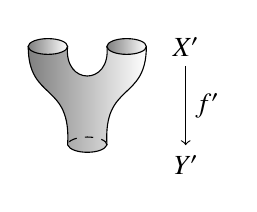
\begin{tikzpicture}[scale=.5]
    \multc
    \node (Y) at (2.5,-.5) {$Y'$};
    \node (X) at (2.5,2.5) {$X'$}
      edge [->] node [right] {$f'$} (Y);
  \end{tikzpicture}
\end{center}
is this:
\begin{center}
  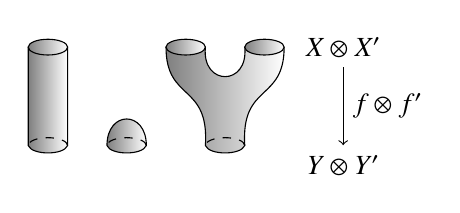
\begin{tikzpicture}[scale=.5]
    \identc
    \begin{scope}[xshift=2cm]
      \birthc
    \end{scope}
    \begin{scope}[xshift=4.5cm]
      \multc
    \end{scope}
    \node (Y) at (7.5,-.5) {$Y \otimes Y'$};
    \node (X) at (7.5,2.5) {$X \otimes X'$}
      edge [->] node [right] {$f \otimes f'$} (Y);
  \end{tikzpicture}
\end{center}

\item The category $\Tang_k$ is monoidal when $k \ge 1$, where the the tensor product is given by disjoint union.  For example, given these two tangles:
\[
\text{\epsfysize=1.2in\epsfbox{2dtangle.eps}} 
\quad
 \xy
 {\ar_{f} (0,30)*+{X}; (0,0)*+{Y}};
 \endxy
\qquad \qquad
\text{\epsfysize=1.2in\epsfbox{another2dtangle.eps}}
\quad
 \xy
 {\ar_{f'} (0,30)*+{X'}; (0,0)*+{Y'}};
 \endxy
\]
their tensor product looks like this:
\[  
\epsfysize=1.2in\epsfbox{tensortangle.eps}
\quad
 \xy
 {\ar_{f \tensor f'} (0,30)*+{X \tensor X'}; (0,0)*+{Y \tensor Y'}};
 \endxy
\]
\end{itemize}

The example of $\Set$ with its cartesian product is different from our other three main examples, because the cartesian product of sets 
$X \times X'$ comes equipped with functions called `projections' to the sets $X$ and $X'$:
\[    
\begin{diagram}
\node{X} \node{X \times X'} \arrow{w,t}{p} \arrow{e,t}{p'} \node{X'}
\end{diagram}
\]
Our other main examples lack this feature --- though $\Hilb$ made into a monoidal category using $\oplus$ has projections. Also, every set has a unique function to the one-element set:
\[           !_X \maps X \to I. \]
Again, our other main examples lack this feature, though $\Hilb$ made into a monoidal category using $\oplus$ has it.  A fascinating feature of quantum mechanics is that we make $\Hilb$ into a monoidal category using $\tensor$ instead of $\oplus$, even though the latter approach would lead to a category more like $\Set$.

We can isolate the special features of the cartesian product of sets and its projections, obtaining a definition that applies to any category:

\begin{definition}
Given objects $X$ and $X'$ in some category, we say an object $X \times X'$ equipped with morphisms 
\[    
\begin{diagram}
\node{X} \node{X \times X'} \arrow{w,t}{p} \arrow{e,t}{p'} \node{X'}
\end{diagram}
\]
is a {\bf cartesian product} (or simply {\bf product}) of $X$ and $X'$ 
if for any object $Q$ and morphisms 
\[          
\begin{diagram}
\node[2]{Q} \arrow{sw,t}{f} \arrow{se,t}{f'}  \\
\node{X} \node[2]{X'}
\end{diagram}
\]
there exists a unique morphism $g \maps Q \to X \times X'$ making the following diagram commute:
\[          
\begin{diagram}
\node[2]{Q} \arrow{sw,t}{f} \arrow{se,t}{f'} 
\arrow{s,r}{g} \\
\node{X} \node{X \times X'} \arrow{w,b}{p} \arrow{e,b}{p'} \node{X'}
\end{diagram}
\]
(That is, $f = p g$ and $f' = p' g$.)  We say a category has
{\bf binary products} if every pair of objects has a product.
\end{definition}
\noindent The product may not exist, and it may not be unique, but when it exists it is unique up to a canonical isomorphism.  This justifies our speaking of `the' product of objects $X$ and $Y$ when it exists, and denoting it as $X \times Y$.

The definition of cartesian product, while absolutely fundamental, is a bit scary at first sight.  To illustrate its power, let us do something with it: combine two morphisms $f \maps X \to Y$ and $f'
\maps X' \to Y'$ into a single morphism
\[   f \times f' \maps X \times X' \to Y \times Y'. \]
The definition of cartesian product says how to build a morphism of this sort out of a pair of morphisms: namely, morphisms from $X \times X'$ to $Y$ and $Y'$.  If we take these to be $f p$ and $f' p'$, we obtain $f \times f'$:
\[          
\begin{diagram}
\node[2]{X \times X'} \arrow{sw,t}{fp} \arrow{se,t}{f'p'} 
\arrow{s,r}{f \times f'} \\
\node{Y} \node{Y \times Y'} \arrow{w,t}{p} \arrow{e,t}{p'} \node{Y'}
\end{diagram}
\]

Next, let us isolate the special features of the one-element set:

\begin{definition}
An object $1$ in a category $C$ is {\bf terminal} if for any object
$Q \in C$ there exists a unique morphism from $Q$ to $1$, which we denote as $!_Q \maps Q \to 1$.
\end{definition}
\noindent Again, a terminal object may not exist and may not be unique, but it is unique up to a canonical isomorphism.  This is why we can speak of `the'
terminal object of a category, and denote it by a specific symbol, $1$.

We have introduced the concept of binary products.  One can also talk about $n$-ary products for other values of $n$, but a category with binary products has $n$-ary products for all $n \ge 1$, since we can construct these as iterated binary products.  The case $n = 1$ is trivial, since the product of one object is just that object itself
(up to canonical isomorphism).  The remaining case is $n = 0$.  The zero-ary product of objects, if it exists, is just the terminal object. So, we make the following definition:

\begin{definition} 
\label{finite_products}
A category has {\bf finite products} if it has binary products and a terminal object.  
\end{definition}
\noindent A category with finite products can always be made into a monoidal category by choosing a specific product $X \times Y$ to be the tensor product $X \tensor Y$, and choosing a specific terminal object to be the unit object.  It takes a bit of work to show this!  A
monoidal category of this form is called {\bf cartesian}.

In a cartesian category, we can `duplicate and delete information'. In general, the definition of cartesian products gives a way to take two morphisms $f_1 \maps Q \to X$ and $f_2 \maps Q \to Y$ and combine them into a single morphism from $Q$ to $X \times Y$.  If we take $Q = X = Y$ and take $f_1$ and $f_2$ to be the identity, we obtain the {\bf diagonal}
or {\bf duplication} morphism:
\[         \Delta_X \maps X \to X \times X.  \]
In the category $\Set$ one can check that this maps any element $x \in X$ to the pair $(x,x)$.  In general, we can draw the diagonal as follows:
\[\begin{pspicture}(0,0)(2,4)
\psset{angleA=-90,angleB=90,ArrowInside=->,arrowscale=2}
\pnode(1,4){A}
\pnode(0,0){B1}
\pnode(2,0){B2}
\rput(1,2){\ovalnode{D}{$\Delta$}}
\nccurve{A}{D}\nbput{$X$}
\nccurve[angleA=-135]{D}{B1}\nbput{$X$}
\nccurve[angleA=-45]{D}{B2}\naput{$X$}
\end{pspicture}\]
Similarly, we call the unique map to the terminal object
\[      !_X \maps X \to 1  \]
the {\bf deletion} morphism, and draw it as follows:
\[\begin{pspicture}(0,0)(2,3)
\psset{angleA=-90,angleB=90,ArrowInside=->,arrowscale=2}
\pnode(1,3){A}
\rput(1,1){\ovalnode{D}{!}}
\nccurve{A}{D}\nbput{$X$}
\end{pspicture}\]
Note that we draw the unit object as an empty space.

A fundamental fact about cartesian categories is that duplicating something and then deleting either copy is the same as doing nothing at all!  In string diagrams, this says:
\[\begin{pspicture}(0,0)(8,7)
  \psset{angleA=-90,angleB=90,ArrowInside=->,arrowscale=2}
  \pnode(1,7){A}
  \rput(0,3){\ovalnode{B1}{!}}
  \pnode(2,3){B2}
  \rput(1,5){\ovalnode{D}{$\Delta$}}
  \nccurve{A}{D}\nbput{$X$}
  \nccurve[angleA=-135]{D}{B1}\nbput{$X$}
  \nccurve[angleA=-45,ArrowInside=-]{D}{B2}\naput{$X$}
  \pnode(2,1){B3}
  \nccurve{B2}{B3}    
  
  \rput(3,5){$=$}
  
  \pnode(5,7){A}
  \pnode(5,1){B}
  \nccurve{A}{B} \nbput{$X$}
  
  \rput(7,5){$=$}
  
  \pnode(9,7){A}
  \pnode(8,3){B1}
  \rput(10,3){\ovalnode{B2}{!}}
  \rput(9,5){\ovalnode{D}{$\Delta$}}
  \nccurve{A}{D}\nbput{$X$}
  \nccurve[angleA=-135]{D}{B1}\nbput{$X$}
  \nccurve[angleA=-45,ArrowInside=-]{D}{B2}\naput{$X$}
  \pnode(8,1){B3}
  \nccurve{B1}{B3}    
\end{pspicture}\]
We leave the proof as an exercise for the reader.

Many of the puzzling features of quantum theory come from the noncartesianness of the usual tensor product in $\Hilb$. For example, in a cartesian category, every morphism 
\[\begin{pspicture}(0,0)(4,3)
\psset{angleA=-90,angleB=90,ArrowInside=->,arrowscale=2}
    \rput(2,2){\ovalnode{F}{$g$}}
    \pnode(1,0){Y1}
    \pnode(3,0){Y2}
    \nccurve[angleA=-120]{F}{Y1} \nbput[npos=1]{$X$}
    \nccurve[angleA=-60]{F}{Y2} \naput[npos=1]{$X'$}
\end{pspicture}\]
is actually of the form 
\[\begin{pspicture}(0,0)(4,3)
\psset{angleA=-90,angleB=90,ArrowInside=->,arrowscale=2}
\pnode(1,4){A}
\rput(1,2){\ovalnode{B}{$f$}}
\pnode(1,0){C}
\nccurve{B}{C} \nbput{$X$}
\rput(3,2){\ovalnode{B}{$f'$}}
\pnode(3,0){C}
\nccurve{B}{C} \naput{$X'$}
\end{pspicture}\]
In the case of $\Set$, this says that every point of the set $X \times X'$
comes from a point of $X$ and a point of $X'$.  In physics, this would say that every state $g$ of the combined system $X \tensor X'$ 
is built by combining states of the systems $X$ and $X'$. Bell's theorem \cite{JSBell} says that is {\it not} true in quantum theory.   The reason is that quantum theory uses the noncartesian monoidal category $\Hilb$!

Also, in quantum theory we {\it cannot} freely duplicate or delete information.  Wootters and Zurek \cite{WZ} proved a precise theorem to this effect, focused on duplication: the `no-cloning theorem'.  One can also prove a `no-deletion theorem'.  Again, these results rely on the noncartesian tensor product in $\Hilb$.

\subsection{Braided Monoidal Categories}
\label{braided}

In physics, there is often a process that lets us `switch' two systems by moving them around each other.  In topology, there is a tangle that describes the process of switching two points:
\begin{center}
\epsfysize=1.2in\epsfbox{braid.eps} 
\end{center}
In logic, we can switch the order of two statements in a conjunction:
the statement `$X$ and $Y$' is isomorphic to `$Y$ and $X$'.  In computation, there is a simple program that switches the order of two pieces of data.  A monoidal category in which we can do this sort of thing is called `braided':

\begin{definition} A {\bf braided monoidal category} consists of:
\begin{itemize} 
\item a monoidal category $C$,
\item a natural isomorphism called the {\bf braiding} 
that assigns to every pair of objects $X, Y \in C$ an isomorphism
    \[b_{X,Y} \maps X\tensor Y \to Y \tensor X, \]
\end{itemize}
such that the {\bf hexagon equations} hold:
\[
    \begin{diagram}
 \node{X \tensor (Y \tensor Z)} \arrow{e,t}{a^{-1}_{X,Y,Z}} \arrow{s,l}{b_{X, Y\tensor Z}} 
 \node{(X \tensor Y) \tensor Z} \arrow{e,t}{b_{X,Y}\tensor 1_Z} 
 \node{(Y \tensor X) \tensor Z} \arrow{s,r}{a_{Y,X,Z}}\\
 \node{(Y \tensor Z) \tensor X} 
 \node{Y \tensor (Z \tensor X)} \arrow{w,b}{a^{-1}_{Y,Z,X}} 
 \node{Y\tensor (X\tensor Z)} \arrow{w,b}{1_Y \tensor b_{X, Z}}
\\
 \node{(X\tensor Y)\tensor Z} \arrow{e,t}{a_{X,Y,Z}} \arrow{s,l}{b_{X\tensor Y,Z}} 
 \node{X \tensor(Y\tensor Z)} \arrow{e,t}{1_X \tensor b_{Y,Z}} 
 \node{X \tensor(Z\tensor Y)} \arrow{s,r}{a^{-1}_{X,Z,Y}}\\
 \node{Z \tensor (X \tensor Y)} 
 \node{(Z \tensor X) \tensor Y} \arrow{w,b}{a_{Z,X,Y}} 
 \node{(X \tensor Z) \tensor Y} \arrow{w,b}{b_{Z, X}\tensor 1_Y} 
    \end{diagram}
\]
\end{definition}
\noindent The first hexagon equation says that switching the object $X$ past 
$Y \tensor Z$ all at once is the same as switching it past $Y$ and then past $Z$ (with some associators thrown in to move the parentheses). The second one is similar: it says switching $X \tensor Y$ past $Z$ 
all at once is the same as doing it in two steps.

In string diagrams, we draw the braiding $b_{X,Y} \maps X \tensor Y \to Y \tensor X$ like this:
\[\begin{pspicture}(0,0)(2,3)
\psset{angleA=-90,angleB=90,ArrowInside=->,arrowscale=2}
\pnode(0,2){A1}
\pnode(0,0){B1}
\pnode(1,2){A2}
\pnode(1,0){B2}
\nccurve[ArrowInsidePos=.25]{A1}{B2} \nbput[npos=0]{$X$} \ncput{\cnode[linecolor=white,fillstyle=solid,fillcolor=white]{4pt}{C}}
\nccurve[ArrowInsidePos=.25]{A2}{B1} \naput[npos=0]{$Y$}
\end{pspicture}\]
We draw its inverse $b_{X,Y}^{-1}$ like this:
\[\begin{pspicture}(0,0)(2,3)
\psset{angleA=-90,angleB=90,ArrowInside=->,arrowscale=2}
\pnode(0,2){A1}
\pnode(0,0){B1}
\pnode(1,2){A2}
\pnode(1,0){B2}
\nccurve[ArrowInsidePos=.25]{A2}{B1} \naput[npos=0]{$Y$} \ncput{\cnode[linecolor=white,fillstyle=solid,fillcolor=white]{4pt}{C}}
\nccurve[ArrowInsidePos=.25]{A1}{B2} \nbput[npos=0]{$X$} 
\end{pspicture}\]
This is a nice notation, because it makes the equations saying that $b_{X,Y}$ and $b_{X,Y}^{-1}$ are inverses 
`topologically true':
\[\begin{pspicture}(0,0)(2,5)
\psset{angleA=-90,angleB=90,ArrowInside=->,arrowscale=2}
\pnode(0,4){A1}
\pnode(0,2){A2}
\pnode(0,0){A3}
\pnode(1,4){B1}
\pnode(1,2){B2}
\pnode(1,0){B3}
\nccurve[ArrowInsidePos=.25]{A1}{B2} \nbput[npos=0]{$X$} \ncput{\cnode[linecolor=white,fillstyle=solid,fillcolor=white]{4pt}{C}}
\nccurve[ArrowInsidePos=.25]{B2}{A3} \nbput[npos=1]{$X$} \ncput{\cnode[linecolor=white,fillstyle=solid,fillcolor=white]{4pt}{C}}
\nccurve[ArrowInsidePos=.25]{B1}{A2} \naput[npos=0]{$Y$} 
\nccurve[ArrowInsidePos=.25]{A2}{B3} \naput[npos=1]{$Y$} 
\end{pspicture} \begin{pspicture}(0,0)(2,5)
\rput(0.5,2){=}
\end{pspicture} \begin{pspicture}(0,0)(2,5)
\psset{angleA=-90,angleB=90,ArrowInside=->,arrowscale=2}
\pnode(0,4){A1}
\pnode(0,0){A3}
\pnode(1,4){B1}
\pnode(1,0){B3}
\nccurve{A1}{A3} \nbput{$X$} 
\nccurve{B1}{B3} \naput{$Y$}
\end{pspicture} \begin{pspicture}(0,0)(2,5)
\rput(0.5,2){=}
\end{pspicture} \begin{pspicture}(0,0)(2,5)
\psset{angleA=-90,angleB=90,ArrowInside=->,arrowscale=2}
\pnode(0,4){A1}
\pnode(0,2){A2}
\pnode(0,0){A3}
\pnode(1,4){B1}
\pnode(1,2){B2}
\pnode(1,0){B3}
\nccurve[ArrowInsidePos=.25]{B1}{A2} \naput[npos=0]{$Y$} \ncput{\cnode[linecolor=white,fillstyle=solid,fillcolor=white]{4pt}{C}}
\nccurve[ArrowInsidePos=.25]{A2}{B3} \naput[npos=1]{$Y$} \ncput{\cnode[linecolor=white,fillstyle=solid,fillcolor=white]{4pt}{C}}
\nccurve[ArrowInsidePos=.25]{A1}{B2} \nbput[npos=0]{$X$} 
\nccurve[ArrowInsidePos=.25]{B2}{A3} \nbput[npos=1]{$X$} 
\end{pspicture}\]

Here are the hexagon equations as string diagrams:
\[\begin{pspicture}(0,0)(2,5)
  \psset{angleA=-90,angleB=90,ArrowInside=->,arrowscale=2}
  \pnode(0,4){A1}
  \pnode(2,4){B1}
  \pnode(0,0){A3}
  \pnode(2,0){B3}
  \nccurve[ArrowInsidePos=.4]{A1}{B3} \nbput[npos=0]{$X$} \naput[npos=1]{$X$} \ncput{\cnode[linecolor=white,fillstyle=solid,fillcolor=white]{4pt}{C}} 
  \nccurve[ArrowInsidePos=.4]{B1}{A3} \naput[npos=0]{$Y\tensor Z$} \nbput[npos=1]{$Y\tensor Z$}
  \end{pspicture} \begin{pspicture}(0,0)(4,5)
  \rput(2,2){=}
  \end{pspicture} \begin{pspicture}(0,0)(2,5)
  \psset{angleA=-90,angleB=90,ArrowInside=->,arrowscale=2}
  \pnode(0,4){A1}
  \pnode(1,4){B1}
  \pnode(2,4){C1}
  \pnode(0,2){A2}
  \pnode(1,2){B2}
  \pnode(2,2){C2}
  \pnode(0,0){A3}
  \pnode(1,0){B3}
  \pnode(2,0){C3}
  \nccurve[ArrowInsidePos=1]{A1}{B2} \nbput[npos=0]{$X$} \ncput{\cnode[linecolor=white,fillstyle=solid,fillcolor=white]{4pt}{C}}
  \nccurve[ArrowInsidePos=1]{B1}{A2} \naput[npos=0]{$Y$} 
  \nccurve[ArrowInsidePos=1]{C1}{C2} \naput[npos=0]{$Z$} 
  \nccurve[ArrowInside=]{A2}{A3} \nbput[npos=1]{$Y$} 
  \nccurve[ArrowInside=]{B2}{C3} \naput[npos=1]{$X$} \ncput{\cnode[linecolor=white,fillstyle=solid,fillcolor=white]{4pt}{C}}
  \nccurve[ArrowInside=]{C2}{B3} \nbput[npos=1]{$Z$}
\end{pspicture}\]

\[\begin{pspicture}(0,0)(2,5)
  \psset{angleA=-90,angleB=90,ArrowInside=->,arrowscale=2}
  \pnode(0,4){A1}
  \pnode(2,4){B1}
  \pnode(0,0){A3}
  \pnode(2,0){B3}
  \nccurve[ArrowInsidePos=.4]{A1}{B3} \nbput[npos=0]{$X\tensor Y$} \naput[npos=1]{$X\tensor Y$} \ncput{\cnode[linecolor=white,fillstyle=solid,fillcolor=white]{4pt}{C}}
  \nccurve[ArrowInsidePos=.4]{B1}{A3} \naput[npos=0]{$Z$} \nbput[npos=1]{$Z$} 
  \end{pspicture} \begin{pspicture}(0,0)(4,5)
  \rput(2,2){=}
  \end{pspicture} \begin{pspicture}(0,0)(2,5)
  \psset{angleA=-90,angleB=90,ArrowInside=->,arrowscale=2}
  \pnode(0,4){A1}
  \pnode(1,4){B1}
  \pnode(2,4){C1}
  \pnode(0,2){A2}
  \pnode(1,2){B2}
  \pnode(2,2){C2}
  \pnode(0,0){A3}
  \pnode(1,0){B3}
  \pnode(2,0){C3}
  \nccurve[ArrowInsidePos=1]{B1}{C2} \nbput[npos=0]{$Y$} \ncput{\cnode[linecolor=white,fillstyle=solid,fillcolor=white]{4pt}{C}}
  \nccurve[ArrowInsidePos=1]{C1}{B2} \naput[npos=0]{$Z$} 
  \nccurve[ArrowInsidePos=1]{A1}{A2} \nbput[npos=0]{$X$} 
  \nccurve[ArrowInside=]{C2}{C3} \naput[npos=1]{$Y$} 
  \nccurve[ArrowInside=]{A2}{B3} \naput[npos=1]{$X$} \ncput{\cnode[linecolor=white,fillstyle=solid,fillcolor=white]{4pt}{C}}
  \nccurve[ArrowInside=]{B2}{A3} \nbput[npos=1]{$Z$}
\end{pspicture}\]

For practice, we urge you to prove the following equations:
\[\begin{pspicture}(0,0)(2,5)
  \psset{angleA=-90,angleB=90,ArrowInside=->,arrowscale=2}
  \pnode(0,4){A1}
  \rput(0,3){\ovalnode{F}{$f$}}
  \pnode(0,2){A2}
  \pnode(0,0){A3}
  \pnode(1,4){B1}
  \rput(1,3){\ovalnode{G}{$g$}}
  \pnode(1,2){B2}
  \pnode(1,0){B3}
  \nccurve[ArrowInsidePos=.75]{A1}{F} \nbput[npos=0]{$X$}
  \nccurve[ArrowInside=]{F}{A2}
  \nccurve[ArrowInsidePos=.25]{A2}{B3} \naput[npos=1]{$X'$} \ncput{\cnode[linecolor=white,fillstyle=solid,fillcolor=white]{4pt}{C}}
  \nccurve[ArrowInsidePos=.75]{B1}{G} \naput[npos=0]{$Y$}
  \nccurve[ArrowInside=]{G}{B2}
  \nccurve[ArrowInsidePos=.25]{B2}{A3} \nbput[npos=1]{$Y'$}
  \end{pspicture} \begin{pspicture}(0,0)(2,5)
  \rput(0.5,2){=}
  \end{pspicture} \begin{pspicture}(0,0)(1,5)
  \psset{angleA=-90,angleB=90,ArrowInside=->,arrowscale=2}
  \pnode(0,4){A1}
  \pnode(0,2){A2}
  \rput(0,1){\ovalnode{G}{$g$}}
  \pnode(0,0){A3}
  \pnode(1,4){B1}
  \pnode(1,2){B2}
  \rput(1,1){\ovalnode{F}{$f$}}
  \pnode(1,0){B3}
  \nccurve[ArrowInsidePos=.75]{A1}{B2} \nbput[npos=0]{$X$} \ncput{\cnode[linecolor=white,fillstyle=solid,fillcolor=white]{4pt}{C}}
  \nccurve[ArrowInside=]{B2}{F}
  \nccurve[ArrowInsidePos=.75]{F}{B3} \naput[npos=1]{$X'$}
  \nccurve[ArrowInsidePos=.75]{B1}{A2} \naput[npos=0]{$Y$}
  \nccurve[ArrowInside=]{A2}{G}
  \nccurve[ArrowInsidePos=.75]{G}{A3} \nbput[npos=1]{$Y'$}
\end{pspicture}\]
\[\begin{pspicture}(0,0)(2,7)
\psset{angleA=-90,angleB=90,ArrowInside=->,arrowscale=2}
\pnode(0,6){A1}
\pnode(1,6){B1}
\pnode(2,6){C1}
\pnode(0,4){A2}
\pnode(1,4){B2}
\pnode(2,4){C2}
\pnode(0,2){A3}
\pnode(1,2){B3}
\pnode(2,2){C3}
\pnode(0,0){A4}
\pnode(1,0){B4}
\pnode(2,0){C4}
\nccurve[ArrowInsidePos=1]{C1}{C2} \naput[npos=0]{$Z$} 
\nccurve[ArrowInsidePos=1]{A1}{B2} \nbput[npos=0]{$X$} \ncput{\cnode[linecolor=white,fillstyle=solid,fillcolor=white]{4pt}{C}}
\nccurve[ArrowInsidePos=1]{B1}{A2} \nbput[npos=0]{$Y$}
\nccurve[ArrowInsidePos=1]{B2}{C3} \ncput{\cnode[linecolor=white,fillstyle=solid,fillcolor=white]{4pt}{C}}
\nccurve[ArrowInsidePos=1]{C2}{B3} 
\nccurve[ArrowInsidePos=1]{A2}{A3} 
\nccurve[ArrowInside=]{C3}{C4} \naput[npos=1]{$X$} 
\nccurve[ArrowInside=]{A3}{B4} \nbput[npos=1]{$Y$} \ncput{\cnode[linecolor=white,fillstyle=solid,fillcolor=white]{4pt}{C}}
\nccurve[ArrowInside=]{B3}{A4} \nbput[npos=1]{$Z$}
\end{pspicture} \begin{pspicture}(0,0)(4,5)
\rput(2,3){=}
\end{pspicture} \begin{pspicture}(0,0)(2,7)
\psset{angleA=-90,angleB=90,ArrowInside=->,arrowscale=2}
\pnode(0,6){A1}
\pnode(1,6){B1}
\pnode(2,6){C1}
\pnode(0,4){A2}
\pnode(1,4){B2}
\pnode(2,4){C2}
\pnode(0,2){A3}
\pnode(1,2){B3}
\pnode(2,2){C3}
\pnode(0,0){A4}
\pnode(1,0){B4}
\pnode(2,0){C4}
\nccurve[ArrowInsidePos=1]{B1}{C2} \nbput[npos=0]{$Y$} \ncput{\cnode[linecolor=white,fillstyle=solid,fillcolor=white]{4pt}{C}}
\nccurve[ArrowInsidePos=1]{C1}{B2} \naput[npos=0]{$Z$} 
\nccurve[ArrowInsidePos=1]{A1}{A2} \nbput[npos=0]{$X$}
\nccurve[ArrowInsidePos=1]{C2}{C3} 
\nccurve[ArrowInsidePos=1]{A2}{B3} \ncput{\cnode[linecolor=white,fillstyle=solid,fillcolor=white]{4pt}{C}}
\nccurve[ArrowInsidePos=1]{B2}{A3} 
\nccurve[ArrowInside=]{B3}{C4} \naput[npos=1]{$X$} \ncput{\cnode[linecolor=white,fillstyle=solid,fillcolor=white]{4pt}{C}}
\nccurve[ArrowInside=]{C3}{B4} \nbput[npos=1]{$Y$} 
\nccurve[ArrowInside=]{A3}{A4} \nbput[npos=1]{$Z$}
\end{pspicture}\]
If you get stuck, here are some hints.  The first equation follows from the naturality of the braiding.  The second is called the {\bf Yang--Baxter equation} and follows from a combination of naturality and the hexagon equations \cite{JS1}.

Next, here are some examples.  There can be many different ways to give a monoidal category a braiding, or none.  However, most of our favorite examples come with well-known `standard' braidings:

\begin{itemize}
\item Any cartesian category automatically becomes braided, and in $\Set$ with its cartesian product, this standard braiding is given by:
\[
\begin{array}{rccl}
        b_{X,Y} & \maps X\times Y& \to& Y\times X \\
                    & (x,y) &\mapsto & (y,x) .
\end{array}
\]
\item In $\Hilb$ with its usual tensor product, the standard braiding is given by:
\[
\begin{array}{rccl}
        b_{X,Y} & \maps X\tensor Y& \to& Y\tensor X \\
                    & x \tensor y &\mapsto & y \tensor x .
\end{array}
\]
\item The monoidal category $n\Cob$ has a standard braiding where
$b_{X,Y}$ is diffeomorphic to the disjoint union of cylinders $X
\times [0,1]$ and $Y \times [0,1]$.  For $2\Cob$ this braiding looks as follows when $X$ and $Y$ are circles:
\begin{center}
  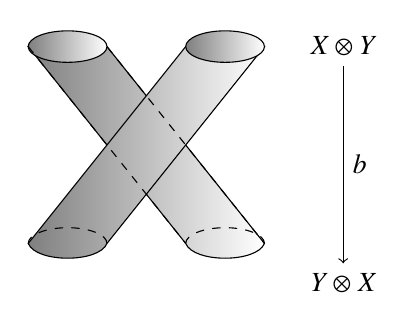
\begin{tikzpicture}
    \ucrossc
    \node (B) at (2.5,-.5) {$Y \tensor X$};
    \node at (2.5, 2.5) {$X \tensor Y$}
      edge [->] node [right] {$b$} (B);
  \end{tikzpicture}
\end{center}

\item The monoidal category $\Tang_k$ has a standard braiding when $k \ge 2$.  For $k = 2$ this looks as follows when $X$ and 
$Y$ are each a single point:
\begin{center}
\epsfysize=1.2in\epsfbox{braid.eps}
\qquad
$
 \xy
 {\ar_{b_{X,Y}} (0,32)*+{X \tensor Y}; (0,-2)*+{Y \tensor X}};
 \endxy
$
\end{center}
\end{itemize}

The example of $\Tang_k$ illustrates an important pattern.  $\Tang_0$ is just a category, because in 0-dimensional space we can only do processes in `series': that is, compose morphisms.  $\Tang_1$ is a monoidal category, because in 1-dimensional space we can also do processes in `parallel': that is, tensor morphisms.  $\Tang_2$ is a braided monoidal category, because in 2-dimensional space there is room to move one object around another.  Next we shall see what happens when space has 3 or more dimensions!

\subsection{Symmetric Monoidal Categories}
\label{symmetric}

Sometimes switching two objects and switching them again is the same as doing nothing at all.  Indeed, this situation is very familiar. So, the first braided monoidal categories to be discovered were
`symmetric' ones \cite{MacLane}:

\begin{definition}
    A {\bf symmetric monoidal category} is a braided monoidal category where the braiding satisfies $b_{X,Y} = b_{Y,X}^{-1}$.
\end{definition}

So, in a symmetric monoidal category, 
\[\begin{pspicture}(0,0)(5,5)
\psset{angleA=-90,angleB=90,ArrowInside=->,arrowscale=2}
\pnode(0,4){A1}
\pnode(1,4){A2}
\pnode(0,2){B1}
\pnode(1,2){B2}
\nccurve[ArrowInsidePos=1]{A1}{B2} \nbput[npos=0]{$X$} \ncput{\cnode[linecolor=white,fillstyle=solid,fillcolor=white]{4pt}{C}}
\nccurve[ArrowInsidePos=1]{A2}{B1} \naput[npos=0]{$Y$}
\pnode(0,2){A1}
\pnode(1,2){A2}
\pnode(0,0){B1}
\pnode(1,0){B2}
\nccurve[ArrowInside=-]{A1}{B2} \naput[npos=1]{$Y$} \ncput{\cnode[linecolor=white,fillstyle=solid,fillcolor=white]{4pt}{C}}
\nccurve[ArrowInside=-]{A2}{B1} \nbput[npos=1]{$X$}

\rput(2.5,2){$=$}

\pnode(4,4){A1}
\pnode(5,4){A2}
\pnode(4,0){B1}
\pnode(5,0){B2}
\nccurve{A1}{B1} \nbput{$X$}
\nccurve{A2}{B2} \naput{$Y$}
\end{pspicture}\]
or equivalently:
\[\begin{pspicture}(0,0)(1,3)
\psset{angleA=-90,angleB=90,ArrowInside=->,arrowscale=2}
\pnode(0,2){A1}
\pnode(1,2){A2}
\pnode(0,0){B1}
\pnode(1,0){B2}
\nccurve[ArrowInsidePos=.25]{A1}{B2} \nbput[npos=0]{$X$} \ncput{\cnode[linecolor=white,fillstyle=solid,fillcolor=white]{4pt}{C}}
\nccurve[ArrowInsidePos=.25]{A2}{B1} \naput[npos=0]{$Y$}
\end{pspicture}
\begin{pspicture}(0,0)(2,2)
\rput(1,1){$=$}
\end{pspicture}
\begin{pspicture}(0,0)(1,2)
\psset{angleA=-90,angleB=90,ArrowInside=->,arrowscale=2}\pnode(0,2){A1}
\pnode(1,2){A2}
\pnode(0,0){B1}
\pnode(1,0){B2}
\nccurve[ArrowInsidePos=.25]{A2}{B1} \naput[npos=0]{$Y$} \ncput{\cnode[linecolor=white,fillstyle=solid,fillcolor=white]{4pt}{C}}
\nccurve[ArrowInsidePos=.25]{A1}{B2} \nbput[npos=0]{$X$} 
\end{pspicture}\]

Any cartesian category automatically becomes a symmetric monoidal category, so $\Set$ is symmetric.  It is also easy to check that
$\Hilb$, $n\Cob$ are symmetric monoidal categories.  So is $\Tang_k$ 
for $k \ge 3$.   

Interestingly, $\Tang_k$ `stabilizes' at $k = 3$: increasing the value of $k$ beyond this value merely gives a category equivalent to
$\Tang_3$.  The reason is that we can already untie all knots in
4-dimensional space; adding extra dimensions has no real effect. In fact, $\Tang_k$ for $k \ge 3$ is equivalent to $1\Cob$. This is part of a conjectured larger pattern called the `Periodic Table' of $n$-categories \cite{HDATQFT}.  A piece of this is shown in Table \ref{periodic_table}.

An $n$-category has not only morphisms going between objects, but 
2-morphisms going between morphisms, 3-morphisms going between 
2-morphisms and so on up to $n$-morphisms.  In topology we can use $n$-categories to describe tangled higher-dimensional surfaces
\cite{HDA4}, and in physics we can use them to describe not just particles but also strings and higher-dimensional membranes \cite{HDATQFT,BL}. The Rosetta Stone we are describing concerns only the $n = 1$ column of the Periodic Table.   So, it is probably just a fragment of a larger, still buried $n$-categorical Rosetta Stone.  We examine the $n=2$ column in Part III of this thesis.

\begin{table}[h]
\begin{center}
\begin{tabular}{|c|c|c|c|}  \hline
        & $\mathbf{\mathit n = 0}$ & $\mathbf{\mathit n = 1}$ &
$\mathbf{\mathit n = 2}$\\ \hline $\mathbf{\mathit k = 0}$ & sets
& categories & 2-categories     \\     \hline
$\mathbf{\mathit k = 1}$  & monoids   & monoidal   & monoidal         \\
        &           & categories & 2-categories     \\     \hline
$\mathbf{\mathit k = 2}$  &commutative& braided    & braided          \\
        & monoids   & monoidal   & monoidal         \\
        &           & categories & 2-categories     \\     \hline
$\mathbf{\mathit k = 3}$  &`'         & symmetric  & sylleptic \\
        &           & monoidal   & monoidal         \\
        &           & categories & 2-categories     \\     \hline
$\mathbf{\mathit k = 4}$  &`'         & `'         & symmetric \\
        &           &            & monoidal         \\
        &           &            & 2-categories     \\     \hline
$\mathbf{\mathit k = 5}$  &`'         &`'          & `'               \\
        &           &            &                  \\
        &           &            &                  \\     \hline
$\mathbf{\mathit k = 6}$  &`'         &`'          & `'               \\
        &           &            &                  \\
        &           &            &                  \\     \hline
\end{tabular}
\\
\caption{The Periodic Table: conjectured descriptions of $(n+k)$-categories with only one $j$-morphism for $j < k$.}
\label{periodic_table}
\end{center}
\end{table}

\subsection{Closed Categories}
\label{closed}

In quantum mechanics, one can encode a linear operator $f \maps X \to Y$ into a quantum state using a technique called `gate teleportation'
\cite{GC}.  In topology, there is a way to take any tangle $f \maps X
\to Y$ and bend the input back around to make it part of the output. In logic, we can take a proof that goes from some assumption $X$ to some conclusion $Y$ and turn it into a proof that goes from no assumptions to the conclusion `$X$ implies $Y$'.  In computer science, we can take any program that takes input of type $X$ and produces output of type $Y$, and think of it as a piece of data of a new type:
a `function type'.  The underlying concept that unifies all these examples is the concept of a `closed category'.

Given objects $X$ and $Y$ in any category $C$, there is a {\em set} of morphisms from $X$ to $Y$, denoted $\hom(X,Y)$.  In a closed category there is also an {\em object} of morphisms from $X$ to $Y$, which we denote by $X \lhom Y$.  (Many other notations are also used.)  In this situation we speak of an `internal hom', since the object $X \lhom Y$
lives inside $C$, instead of `outside', in the category of sets.

Closed categories were introduced in 1966, by Eilenberg and Kelly \cite{EK}. While these authors were able to define a closed structure for any category, it turns out that the internal hom is most easily understood for monoidal categories.  The reason is that when our category has a tensor product, it is closed precisely when morphisms from $X \tensor Y$
to $Z$ are in natural one-to-one correspondence with morphisms from $Y$
to $X \lhom Z$.  In other words, it is closed when we have a natural isomorphism
\[  
\begin{array}{rcl}       
 \hom(X \tensor Y , Z) &\iso & \hom(Y, X \lhom Z)  \\
                    f &\mapsto & \tilde{f}  
\end{array}
\]
For example, in the category $\Set$, if we take
$X \tensor Y$ to be the cartesian product $X \times Y$, then 
$X \lhom Z$ is just the set of functions from $X$ to $Z$, and we have a one-to-one correspondence between
\begin{itemize}
\item functions $f$ that eat elements of
$X \times Y$ and spit out elements of $Z$ 
\end{itemize}
and 
\begin{itemize}
\item functions $\tilde{f}$ that eat elements of $Y$ and spit out functions from $X$ to $Z$.
\end{itemize}
This correspondence goes as follows:
\[          \tilde{f}(y)(x) = f(x,y)  .\]

Before considering other examples, we should make the definition of `closed monoidal category' completely precise.  For this we must note that for any category $C$, there is a functor
\[            \hom \maps C^{\op} \times C \to \Set  .\]

\begin{definition} The {\bf opposite category} $C^{\op}$ of a category $C$ 
has the same objects as $C$, but a morphism $f \maps x \to y$ in $C^{\op}$ is a morphism $f \maps y \to x$ in $C$, and the composite $gf$ in
$C^{\op}$ is the composite $fg$ in $C$.  \end{definition}

\begin{definition} 
\label{hom.functor}
For any category $C$, the {\bf hom functor}
\[       \hom \maps C^\op \times C \to \Set  \]
sends any object $(X,Y) \in C^\op \times C$ to the set $\hom(X,Y)$, and sends any morphism $(f,g) \in C^\op \times C$ to the function
\[ 
\begin{array}{rrcl}
\hom(f,g) \maps & \hom(X,Y) & \to     & \hom(X',Y')\\
                & h         & \mapsto & ghf
\end{array}
\]
when $f\maps X' \to X$ and $g\maps Y \to Y'$ are morphisms in $C$.
\end{definition}

\begin{definition}
\label{closed.definition}
A monoidal category $C$ is {\bf left closed} if there is an
{\bf internal hom} functor
\[     \lhom \maps C^\op \times C \to C \]
together with a natural isomorphism $c$ called
{\bf currying} that assigns to any objects $X, Y, Z \in C$ 
a bijection
\[ \begin{array}{rrcl}
 c_{X,Y,Z} \maps & \hom(X\tensor Y, Z) & \isoto & \hom(X,Y \lhom Z)  
\end{array}
\]
It is {\bf right closed} if there is an internal hom functor as above and a natural isomorphism
\[ \begin{array}{rrcl}
 c_{X,Y,Z} \maps & \hom(X\tensor Y, Z) & \isoto & \hom(Y,X \lhom Z) . 
\end{array}
\]
\end{definition}
\noindent The term `currying' is mainly used in computer science, after the work of Curry \cite{Curry}.  In the rest of this section we only consider {\it right} closed monoidal categories.   Luckily, there is no real difference between left and right closed for a braided monoidal category, as the braiding gives an isomorphism $X \tensor Y \cong Y \tensor X$.  

All our examples of monoidal categories are closed, but we shall see that, yet again, $\Set$ is different from the rest:

\begin{itemize}
\item The cartesian category $\Set$ is closed, where 
$X \lhom Y$ is just the set of functions from $X$ to $Y$. In $\Set$ or any other cartesian closed category, the internal hom $X \lhom Y$ is usually denoted $Y^X$. To minimize the number of different notations and emphasize analogies between different contexts, we shall not do this:
we shall always use $X \lhom Y$.  To treat $\Set$ as {\it left}
closed, we define the curried version of $f \maps X \times Y \to Z$
as above:
\[        \tilde{f}(x)(y) = f(x,y)  .\]
To treat it as {\it right} closed, we instead define it by
\[        \tilde{f}(y)(x) = f(x,y)  .\]
This looks a bit awkward, but it will be nice for string diagrams.
\item The symmetric monoidal category $\Hilb$ with its usual tensor product is closed, where $X \lhom Y$ is the set of linear operators from $X$ to $Y$, made into a Hilbert space in a standard way.  In this case we have an isomorphism
\[        X \lhom Y \iso X^* \tensor Y \]
where $X^*$ is the dual of the Hilbert space $X$, that is, the set of linear operators $f \maps X \to \mathbb{C}$, made into a Hilbert space in the usual way.  
\item The monoidal category $\Tang_k$ ($k \ge 1$) is closed. As with $\Hilb$, we have
\[        X \lhom Y \iso X^* \tensor Y \]
where $X^*$ is the orientation-reversed version of $X$.
\item The symmetric monoidal category $n\Cob$ is also closed;
again
\[        X \lhom Y \iso X^* \tensor Y \]
where $X^*$ is the $(n-1)$-manifold $X$ with its orientation reversed.
\end{itemize}

Except for $\Set$, all these examples are actually `compact'.  This basically means that $X \lhom Y$ is isomorphic to $X^* \tensor Y$, where
$X^*$ is some object called the `dual' of $X$.  But to make this precise, we need to define the `dual' of an object in an arbitrary monoidal category.

To do this, let us generalize from the case of $\Hilb$.  As already mentioned, each object $X \in \Hilb$ has a dual $X^*$ 
consisting of all linear operators $f \maps X \to I$, where the unit object $I$ is just $\mathbb{C}$.  There is thus a linear operator 
\[
\begin{array}{rccl}
          e_X  \maps & X \tensor X^* & \to    & I  \\
                     & x \tensor f  & \mapsto & f(x)  
\end{array}
\]
called the {\bf counit} of $X$.  Furthermore, the space of all linear operators from $X$ to $Y \in \Hilb$ can be identified with $X^* \tensor Y$. So, there is also a linear operator called the {\bf unit} of $X$:
\[ 
\begin{array}{rccc}
          i_x  \maps & I & \to     & X^* \tensor X \\
                     & c & \mapsto & c\, 1_X  
\end{array}
\]   
sending any complex number $c$ to the corresponding multiple of the identity operator. 

The significance of the unit and counit become clearer if we borrow some ideas from Feynman.  In physics, if 
$X$ is the Hilbert space of internal states of some particle, 
$X^\ast$ is the Hilbert space for the corresponding antiparticle. Feynman realized that it is enlightening to think of antiparticles as particles going backwards in time.  So, we draw a wire labelled by 
$X^\ast$ as a wire labelled by $X$, but with an arrow pointing 
`backwards in time': that is, up instead of down:
\[\begin{pspicture}(0,0)(2.5,2)
 \psset{angleA=-90,angleB=90,ArrowInside=->,arrowscale=2}
 \pnode(0,2){A1}
 \pnode(0,0){B1}
 \pnode(2.5,2){A2}
 \pnode(2.5,0){B2}
 \nccurve{A1}{B1} \nbput{$X^*$}
 \rput(1,1){=}
 \nccurve[angleA=90,angleB=-90]{B2}{A2} \naput{$X$}
 \end{pspicture}\]
(Here we should admit that most physicists use the opposite convention, where time marches up the page.  Since we read from top to bottom, we prefer to let time run down the page.)  

If we draw $X^*$ as $X$ going backwards in time, we can draw the unit as a {\bf cap}:
\[\begin{pspicture}(0,0)(1,2)
  \psset{ArrowInside=->,arrowscale=2}
  \pnode(0,0){A1}
  \pnode(1,0){B1}
  \pnode(.5,1){C1}
  \nccurve[angleA=90,angleB=180]{A1}{C1} \naput[npos=0]{$X$}
  \nccurve[angleA=0,angleB=90]{C1}{B1} \naput[npos=1]{$X$}
\end{pspicture}\]
and the counit as a {\bf cup}:
\[\begin{pspicture}(0,0)(1,2)
  \psset{ArrowInside=->,arrowscale=2}
  \pnode(0,1){A1}
  \pnode(1,1){B1}
  \pnode(.5,0){C1}
  \nccurve[angleA=-90,angleB=180]{A1}{C1} \nbput[npos=0]{$X$}
  \nccurve[angleA=0,angleB=-90]{C1}{B1} \nbput[npos=1]{$X$}
\end{pspicture}\]
In Feynman diagrams, these describe the {\em creation} and
{\em annihilation} of virtual particle-antiparticle pairs!

It then turns out that the unit and counit satisfy two equations, the {\bf zig-zag equations}:
\[\begin{pspicture}(0,0)(2,4)
  \psset{angleA=-90,angleB=90,ArrowInside=->,arrowscale=2}
  \pnode(0,3){A}
  \pnode(.5,1){B}
  \pnode(1,2){C}
  \pnode(1.5,0){D}
  \nccurve[angleB=180]{A}{B} \nbput[npos=0]{$X$}
  \nccurve[angleA=0,angleB=180]{B}{C}
  \nccurve[angleA=0]{C}{D} \nbput[npos=1]{$X$}
  \end{pspicture}
  \begin{pspicture}(0,0)(2,4)\rput(0.5,1.5){=}\end{pspicture}
  \begin{pspicture}(0,0)(1,4)
  \psset{angleA=-90,angleB=90,ArrowInside=->,arrowscale=2}
  \pnode(0,3){A}
  \pnode(0,0){B}
  \nccurve{A}{B} \nbput{$X$}
  \end{pspicture}
\]
\[
  \begin{pspicture}(0,0)(2,4)
  \psset{angleA=90,angleB=-90,ArrowInside=->,arrowscale=2}
  \pnode(1.5,3){A}
  \pnode(1,1){B}
  \pnode(.5,2){C}
  \pnode(0,0){D}
  \nccurve[angleB=180]{D}{C} \naput[npos=0]{$X$}
  \nccurve[angleA=0,angleB=180]{C}{B}
  \nccurve[angleA=0]{B}{A} \naput[npos=1]{$X$}
  \end{pspicture}
  \begin{pspicture}(0,0)(2,4)\rput(0.5,1.5){=}\end{pspicture}
  \begin{pspicture}(0,0)(1,4)
  \psset{angleA=90,angleB=-90,ArrowInside=->,arrowscale=2}
  \pnode(0,3){A}
  \pnode(0,0){B}
  \nccurve{B}{A} \naput{$X$}
  \end{pspicture}
\]
Verifying these is a fun exercise in linear algebra, which we leave to the reader.  If we write these equations as commutative diagrams, we need to include some associators and unitors, and they become a bit intimidating:
\[
    \begin{diagram}
\node{X \tensor I} \arrow{e,t}{1_X \tensor i_X} \arrow{s,l}{r_X} 
\node{X \tensor (X^* \tensor X)} \arrow{e,t}{a^{-1}_{X,X^*,X}}
\node{(X \tensor X^*) \tensor X} \arrow{s,r}{e_X \tensor 1_X}\\
\node{X} \node[2]{I \tensor X} \arrow[2]{w,b}{l_X} 
\\
\node{I \tensor X^*} \arrow{e,t}{i_X \tensor 1_X} \arrow{s,l}{l_X} 
\node{(X^* \tensor X) \tensor X^*} \arrow{e,t}{a_{X^*,X,X^*}}
\node{X^* \tensor (X \tensor X^*)} \arrow{s,r}{1_{X^*} \tensor e_X}\\
\node{X^*} \node[2]{X^* \tensor I} \arrow[2]{w,b}{r_{X^*}} 
    \end{diagram}
\]
But, they really just say that zig-zags in string diagrams can be straightened out.

This is particularly vivid in examples like $\Tang_k$ and $n\Cob$. For example, in $2\Cob$, taking $X$ to be the circle, the unit looks like this:
\begin{center}
  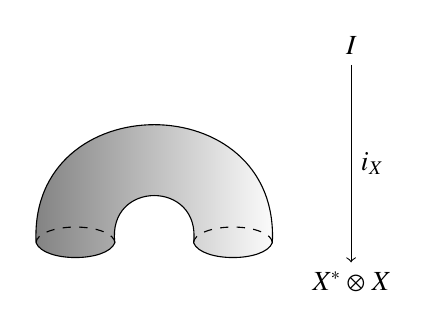
\begin{tikzpicture}
    \zagc
    \node (B) at (2.5, -.5) {$X^* \tensor X$};
    \node at (2.5, 2.5) {$I$}
      edge [->] node [right] {$i_X$} (B);
  \end{tikzpicture}
\end{center}
while the counit looks like this:
\begin{center}
  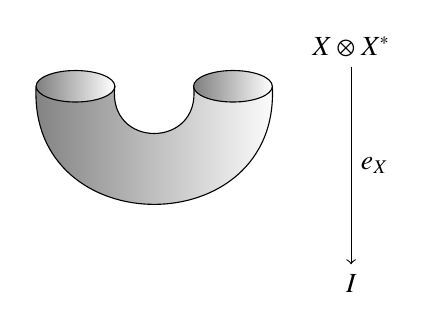
\begin{tikzpicture}
    \zigc
    \node (B) at (2.5, -.5) {$I$};
    \node at (2.5, 2.5) {$X \tensor X^*$}
      edge [->] node [right] {$e_X$} (B);
  \end{tikzpicture}
\end{center}
In this case, the zig-zag identities say we can straighten a wiggly piece of pipe.

Now we are ready for some definitions:

\begin{definition} Given objects $X^*$ and $X$ in a monoidal category, we call $X^*$ a {\bf right dual} of $X$, and $X$ 
a {\bf left dual} of $X^*$, if there are morphisms
\[           i_X \maps I \to X^* \tensor X  \]
and 
\[           e_X \maps X \tensor X^* \to I, \]
called the {\bf unit} and {\bf counit} respectively, satisfying the zig-zag equations.
\end{definition}
One can show that the left or right dual of an object is unique up to canonical isomorphism.   So, we usually speak of `the' right or left dual of an object, when it exists.

\begin{definition} A monoidal category $C$ is {\bf compact}
if every object $X \in C$ has both a left dual and a right dual.
\end{definition}
Often the term `autonomous' is used instead of 
`compact' here.  Many authors reserve the term `compact' for the case where $C$ is symmetric or at least braided; then left duals are the same as right duals, and things simplify \cite{FY}. To add to the confusion, compact symmetric monoidal categories are often called simply `compact closed categories'.

A partial explanation for the last piece of terminology is that any compact monoidal category is automatically closed!   For this, we define the internal hom on objects by
\[                X \lhom Y = X^* \tensor Y  .\]
We must then show that the $*$ operation extends naturally to a functor
$* \maps C \to C$, so that $\lhom$ is actually a functor.  Finally, we must check that there is a natural isomorphism
\[          \hom(X \tensor Y , Z) \cong \hom(Y, X^* \tensor Z) \]
In terms of string diagrams, this isomorphism takes any morphism
\[\begin{pspicture}(0,0)(2,4)
  \psset{angleA=-90,angleB=90,ArrowInside=->,arrowscale=2}
  \pnode(0,4){A}
  \pnode(2,4){B}
  \rput(1,2){\ovalnode{C}{$f$}}
  \pnode(1,0){D}
  \nccurve[angleB=135]{A}{C} \nbput{$X$}
  \nccurve[angleB=45]{B}{C} \naput{$Y$}
  \nccurve{C}{D} \nbput{$Z$}
\end{pspicture}\]
and bends back the input wire labelled $X$ to make it an output:
\[\begin{pspicture}(0,0)(2,4)
  \psset{angleA=-90,angleB=90,ArrowInside=->,arrowscale=2}
  \pnode(0,0){A}
  \pnode(1,4){B}
  \rput(1,2){\ovalnode{C}{$f$}}
  \pnode(2,0){D}
  \nccurve[angleA=90,angleB=135]{A}{C} \naput[npos=.25]{$X$}
  \nccurve[angleB=45]{B}{C} \nbput[npos=.25]{$Y$}
  \nccurve{C}{D} \naput[npos=.75]{$Z$}
\end{pspicture}\]

Now, in a compact monoidal category, we have:
\[\begin{pspicture}(0,0)(4,2)
  \psset{angleA=-90,angleB=90,ArrowInside=->,arrowscale=2}
  \pnode(0,2){A1}
  \pnode(0,0){B1}
  \pnode(1,2){A2}
  \pnode(1,0){B2}
  \nccurve[angleA=90,angleB=-90]{B1}{A1} \naput{$X$}
  \nccurve{A2}{B2} \nbput{$Z$}
  \rput(2,1){=}
  \pnode(3,2){A3}
  \pnode(3,0){B3}
  \nccurve{A3}{B3} \naput{$X\lhom Z$}
\end{pspicture}\]
But in general, closed monoidal categories don't allow arrows pointing up!  So for these, drawing the internal hom is more of a challenge. We can use the same style of notation as long as we add a decoration --- a
{\bf clasp} --- that binds two strings together:
\[\begin{pspicture}(0,0)(4,2)
  \psset{angleA=-90,angleB=90,ArrowInside=->,arrowscale=2}
  \pnode(0,2){A1}
  \pnode(0,0){B1}
  \pnode(1,2){A2}
  \pnode(1,0){B2}
  \nccurve[angleA=90,angleB=-90]{B1}{A1} \naput{$X$} \ncput[npos=.8]{\pnode{A3}}
  \nccurve{A2}{B2} \nbput{$Z$} \ncput[npos=.2]{\cnode{4pt}{B3}}
  \nccurve[angleA=0,angleB=180,ArrowInside=]{A3}{B3}
  \rput(2,1){:=}
  \pnode(3,2){A3}
  \pnode(3,0){B3}
  \nccurve{A3}{B3} \naput{$X\lhom Z$}
\end{pspicture}\]
Only when our closed monoidal category happens to be compact can we eliminate the clasp. 

Suppose we are working in a closed monoidal category. Since we draw a morphism $f \maps X\tensor Y\to Z$ like this:
\[\begin{pspicture}(0,0)(2,4)
  \psset{angleA=-90,angleB=90,ArrowInside=->,arrowscale=2}
  \pnode(0,4){A}
  \pnode(2,4){B}
  \rput(1,2){\ovalnode{C}{$f$}}
  \pnode(1,0){D}
  \nccurve[angleB=135]{A}{C} \nbput{$X$}
  \nccurve[angleB=45]{B}{C} \naput{$Y$}
  \nccurve{C}{D} \nbput{$Z$}
\end{pspicture}\]
we can draw its curried version $\tilde f \maps Y\to X\lhom Z$ by bending down the input wire labelled $X$ to make it part of the output:
\[\begin{pspicture}(0,0)(2,4)
  \psset{angleA=-90,angleB=90,ArrowInside=->,arrowscale=2}
  \pnode(0,0){A}
  \pnode(1,4){B}
  \rput(1,2){\ovalnode{C}{$f$}}
  \pnode(2,0){D}
  \nccurve[angleA=90,angleB=135]{A}{C} \naput[npos=.25]{$X$} \ncput[npos=.25]{\pnode{E}}
  \nccurve[angleB=45]{B}{C} \naput[npos=.25]{$Y$}
  \nccurve{C}{D} \naput[npos=.75]{$Z$} \ncput[npos=.75]{\cnode{4pt}{F}}
  \nccurve[linestyle=none,ArrowInside=-]{C}{C} \ncput{\pscircle{.8}}
  \nccurve[angleA=0,angleB=180,ArrowInside=-]{E}{F}
\end{pspicture}\]
Note that where we bent back the wire labelled $X$, a cap like this appeared:
\[\begin{pspicture}(0,0)(1,1)
  \psset{ArrowInside=->,arrowscale=2}
  \pnode(0,0){A1}
  \pnode(1,0){B1}
  \pnode(.5,1){C1}
  \nccurve[angleA=90,angleB=180]{A1}{C1} \naput[npos=0]{$X$}
  \nccurve[angleA=0,angleB=90]{C1}{B1} \naput[npos=1]{$X$}
\end{pspicture}\]
Closed monoidal categories don't really have a cap unless they are compact.  So, we drew a {\bf bubble} enclosing $f$ and the cap, to keep us from doing any illegal manipulations.  In the compact case, both the bubble and the clasp are unnecessary, so we can draw 
$\tilde{f}$ like this:
\[\begin{pspicture}(0,0)(2,4)
  \psset{angleA=-90,angleB=90,ArrowInside=->,arrowscale=2}
  \pnode(0,0){A}
  \pnode(1,4){B}
  \rput(1,2){\ovalnode{C}{$f$}}
  \pnode(2,0){D}
  \nccurve[angleA=90,angleB=135]{A}{C} \naput[npos=.25]{$X$}
  \nccurve[angleB=45]{B}{C} \nbput[npos=.25]{$Y$}
  \nccurve{C}{D} \naput[npos=.75]{$Z$}
\end{pspicture}\]

An important special case of currying gives the {\bf name} of a morphism
$f \maps X\to Y$, 
\[          \name{f} \maps I \to X \lhom Y .\]
This is obtained by currying the morphism
\[ f r_x \maps I \tensor X \to Y . \]
In string diagrams, we draw $\name{f}$ as follows:
\[\begin{pspicture}(0,0)(1,3)
    \psset{angleA=-90,angleB=90,ArrowInside=->,arrowscale=2}
    \pnode(0,0){A}
    \rput(0.5,2){\ovalnode{C}{$f$}}
    \pnode(1,0){D}
    \nccurve[angleA=90, angleB=135]{A}{C} \naput[npos=.25]{$X$} \ncput[npos=.25]{\pnode{E}}
    \nccurve[angleA=-45]{C}{D} \naput[npos=.75]{$Y$} \ncput[npos=.75]{\cnode{4pt}{F}}
    \nccurve[linestyle=none,ArrowInside=-]{C}{C} \ncput{\pscircle{.8}}
    \nccurve[angleA=0,angleB=180,ArrowInside=-]{E}{F}
\end{pspicture}\]
In the category $\Set$, the unit object is the one-element set, $1$. So, a morphism from this object to a set $Q$ picks out a point of $Q$. In particular, the name $\name{f} \maps 1 \to X \lhom Y$ picks out the element of $X \lhom Y$ corresponding to the function $f \maps X \to Y$.  More generally, in any cartesian closed category the unit object is the terminal object $1$, and a morphism from $1$ to an object $Q$
is called a {\bf point} of $Q$.  So, even in this case, we can say the name of a morphism $f \maps X \to Y$ is a point of $X \lhom Y$.

Something similar works for $\Hilb$, though this example is compact rather than cartesian.  In $\Hilb$, the unit object 
$I$ is just $\CC$.  So, a nonzero morphism from $I$ to any Hilbert space $Q$ picks out a nonzero vector in $Q$, which we can normalize to obtain a {\bf state} in $Q$: that is, a unit vector.  In particular, the name of a nonzero morphism $f \maps X \to Y$ gives a state of
$X^* \tensor Y$.   This method of encoding operators as states is the basis of `gate teleportation' \cite{GC}.

Currying is a bijection, so we can also {\bf uncurry}:
\[ \begin{array}{rrcl}
 c_{X,Y,Z}^{-1} \maps & \hom(Y, X \lhom Z) & \isoto & \hom(X \tensor Y, Z)  \\
                      &         g            & \mapsto    & \utilde{g}   .
\end{array}
\]
Since we draw a morphism $g \maps Y \to X \lhom Z$ like this:
\[\begin{pspicture}(0,0)(3,4)
  \psset{angleA=-90,angleB=90,ArrowInside=->,arrowscale=2}
  \pnode(1,0){A}
  \pnode(2,4){B}
  \rput(2,2){\ovalnode{C}{$g$}}
  \pnode(3,0){D}
  \nccurve[angleA=90,angleB=-135]{A}{C} \naput[npos=.25]{$X$} \ncput[npos=.25]{\pnode{E}}
  \nccurve{B}{C} \naput[npos=.25]{$Y$}
  \nccurve[angleA=-45]{C}{D} \naput{$Z$} \ncput[npos=.75]{\cnode{4pt}{F}}
  \nccurve[angleA=0,angleB=180,ArrowInside=-]{E}{F}
\end{pspicture}\]
we draw its `uncurried' version $\utilde{g} \maps X \tensor Y\to Z $ 
by bending the output $X$ up to become an input:
\[\begin{pspicture}(0,0)(2,4)
  \psset{angleA=-90,angleB=90,ArrowInside=->,arrowscale=2}
  \pnode(0,4){A}
  \pnode(2,4){B}
  \rput(1,2){\ovalnode{C}{$g$}}
  \pnode(1,0){D}
  \nccurve[angleB=-135]{A}{C} \nbput{$X$} \ncput[npos=.9]{\pnode{E}}
  \nccurve{B}{C} \naput{$Y$} 
  \nccurve[angleA=-45,ArrowInsidePos=.75]{C}{D} \nbput[npos=.75]{$Z$} \ncput[npos=.2]{\cnode{4pt}{F}}
  \nccurve[linestyle=none,ArrowInside=-]{C}{C} \ncput{\pscircle{.8}}
  \nccurve[angleA=-90,angleB=180,ArrowInside=-]{E}{F}
\end{pspicture}\]
Again, we must put a bubble around the `cup' formed when we bend down the wire labelled $Y$, unless we are in a compact monoidal category.

A good example of uncurrying is the {\bf evaluation} morphism:
\[ \ev_{X,Y} \maps X \tensor (X\lhom Y) \to Y . \]
This is obtained by uncurrying the identity 
\[          1_{X \lhom Y} \maps (X \lhom Y) \to (X \lhom Y). \]
In $\Set$, $\ev_{X,Y}$ takes any function from $X$ to $Y$ and evaluates it at any element of $X$ to give an element of $Y$. In terms of string diagrams, the evaluation morphism looks like this:
\[\begin{pspicture}(0,0)(3,4)
  \psset{angleA=-90,angleB=90,ArrowInside=->,arrowscale=2}
  \pnode(0,4){A}
  \pnode(2,4){B}
  \pnode(3,4){C}
  \rput(1.5,2){\ovalnode{D}{$\ev$}}
  \pnode(1.5,0){E}
  \nccurve[angleB=144]{A}{D} \nbput{$X$}
  \nccurve[angleA=72,angleB=-90]{D}{B} \naput{$X$}\ncput[npos=0.75]{\pnode{F}}
  \nccurve[angleB=36]{C}{D} \naput{$Y$} \ncput[npos=0.25]{\cnode{4pt}{G}}
  \nccurve{D}{E} \nbput{$Y$}
  \nccurve[angleA=0,angleB=180,ArrowInside=-]{F}{G}
  \end{pspicture}
  \begin{pspicture}(0,0)(2,4)\rput(1,2){=}\end{pspicture}
  \begin{pspicture}(0,0)(3,4)
  \psset{angleA=-90,angleB=90,ArrowInside=->,arrowscale=2}
  \pnode(0,4){A}
  \pnode(2,4){B}
  \pnode(3,4){C}
  \rput(1.5,2){\cnode{24pt}{D}}
  \pnode(1.5,0){E}
  \nccurve[angleB=144]{A}{D} \nbput{$X$} \ncput[npos=1]{\pnode{H}}
  \nccurve[angleA=72,angleB=-90]{D}{B} \naput{$X$}\ncput[npos=0.75]{\pnode{F}} \ncput[npos=0]{\pnode{I}}
  \nccurve[angleB=36]{C}{D} \naput{$Y$} \ncput[npos=0.25]{\cnode{4pt}{G}} \ncput[npos=1]{\pnode{J}}
  \nccurve{D}{E} \nbput{$Y$} \ncput[npos=0]{\pnode{K}}
  \nccurve[angleA=0,angleB=180,ArrowInside=-]{F}{G}
  \psset{ArrowInside=-}
  \nccurve[angleA=-36, angleB=-72]{H}{I}
  \nccurve[angleA=-144]{J}{K}
\end{pspicture}\]

In any closed monoidal category, we can recover a morphism from its name using evaluation.  More precisely, this diagram commutes:
\[
\begin{diagram}
\node{X \tensor I} \arrow{s,l}{1_X \tensor \name{f}}
\node{X} \arrow{w,t}{r^{-1}} \arrow{s,r}{f} \\
\node{X \tensor (X \lhom Y)} \arrow{e,b}{\ev_{X,Y}} \node{Y}
\end{diagram}
\]
Or, in terms of string diagrams:
\[\begin{pspicture}(0,0)(3,8)
  \psset{angleA=-90,angleB=90,ArrowInside=->,arrowscale=2}
  \pnode(0,8){id}
  \rput(2.5,6){\ovalnode{func}{$f$}}
  \rput(2.5,6){\pscircle{.8}}
  \pnode(0,4){A}
  \pnode(2,4){B}
  \pnode(3,4){C}
  \rput(1.5,2){\cnode{24pt}{D}}
  \pnode(1.5,0){E}
  \nccurve{id}{A}
  \nccurve[angleA=90, angleB=135]{B}{func}
  \nccurve[angleA=-45]{func}{C}
  \nccurve[angleB=144]{A}{D} \nbput{$X$} \ncput[npos=1]{\pnode{H}}
  \nccurve[angleA=72,angleB=-90]{D}{B} \naput{$X$}\ncput[npos=0.75]{\pnode{F}} \ncput[npos=0]{\pnode{I}}
  \nccurve[angleB=36]{C}{D} \naput{$Y$} \ncput[npos=0.25]{\cnode{4pt}{G}} \ncput[npos=1]{\pnode{J}}
  \nccurve{D}{E} \nbput{$Y$} \ncput[npos=0]{\pnode{K}}
  \nccurve[angleA=0,angleB=180,ArrowInside=-]{F}{G}
  \psset{ArrowInside=-}
  \nccurve[angleA=-36, angleB=-72]{H}{I}
  \nccurve[angleA=-144]{J}{K}
  \end{pspicture}
  \begin{pspicture}(0,0)(2,8)\rput(2,4){=}\end{pspicture}
  \begin{pspicture}(0,0)(2,8)
  \psset{angleA=-90,angleB=90,ArrowInside=->,arrowscale=2}
  \pnode(1,8){A}
  \rput(1,4){\ovalnode{B}{$f$}}
  \pnode(1,0){C}
  \nccurve{A}{B} \nbput{$X$}
  \nccurve{B}{C} \nbput{$Y$}
\end{pspicture}\]
We leave the proof of this as an exercise.  In general, one must use the naturality of currying.  In the special case of a compact monoidal category, there is a nice picture proof!  Simply pop the bubbles and remove the clasp:
\[\begin{pspicture}(0,0)(3,7)
  \psset{angleA=-90,angleB=90,ArrowInside=->,arrowscale=2}
  \pnode(0,7){id}
  \rput(2.5,6){\ovalnode{func}{$f$}}
  \pnode(0,4){A}
  \pnode(2,4){B}
  \pnode(3,4){C}
  \rput(1.5,2){\cnode[linestyle=none]{24pt}{D}}
  \pnode(1.5,0){E}
  \nccurve{id}{A}
  \nccurve[angleA=90, angleB=135]{B}{func}
  \nccurve[angleA=-45]{func}{C}
  \nccurve[angleB=144]{A}{D} \nbput{$X$} \ncput[npos=1]{\pnode{H}}
  \nccurve[angleA=72,angleB=-90]{D}{B} \naput{$X$}\ncput[npos=0.75]{\pnode{F}} \ncput[npos=0]{\pnode{I}}
  \nccurve[angleB=36]{C}{D} \naput{$Y$} \ncput[npos=1]{\pnode{J}}
  \nccurve{D}{E} \nbput{$Y$} \ncput[npos=0]{\pnode{K}}
  \psset{ArrowInside=-}
  \nccurve[angleA=-36, angleB=-72]{H}{I}
  \nccurve[angleA=-144]{J}{K}
  \end{pspicture}
  \begin{pspicture}(0,0)(2,7)\rput(2,3){=}\end{pspicture}
  \begin{pspicture}(0,0)(2,7)
  \psset{angleA=-90,angleB=90,ArrowInside=->,arrowscale=2}
  \pnode(1,7){A}
  \rput(1,3){\ovalnode{B}{$f$}}
  \pnode(1,0){C}
  \nccurve{A}{B} \nbput{$X$}
  \nccurve{B}{C} \nbput{$Y$}
\end{pspicture}\]
The result then follows from one of the zig-zag identities.  

In our rapid introduction to string diagrams, we have not had time to illustrate how these diagrams become a powerful tool for solving concrete problems.  So, here are some starting points for further study:

\begin{itemize}
\item Representations of Lie groups play a fundamental role in quantum physics, especially gauge field theory. Every Lie group has a compact symmetric monoidal category of finite-dimensional representations.  In his book
{\sl Group Theory}, Cvitanovic \cite{Cvitanovic} develops detailed string diagram descriptions of these representation categories for the classical Lie groups 
$\mathrm{SU}(n)$, $\mathrm{SO}(n)$, $\mathrm{SU}(n)$ and also the more exotic `exceptional' Lie groups. His book also illustrates how this technology can be used to simplify difficult calculations in gauge field theory.
\item Quantum groups are a generalization of groups which show up in 2d and 3d physics.  The big difference is that a quantum group has a compact {\em braided} monoidal category of finite-dimensional representations.  Kauffman's {\sl Knots and Physics} \cite{Kauffman} 
is an excellent introduction to how quantum groups show up in knot theory and physics; it is packed with string diagrams. For more details on quantum groups and braided monoidal categories, see the book by Kassel \cite{Kassel}.
\item Kauffman and Lins \cite{KaufmanLins} have written a beautiful string diagram treatment of the category of representations of the simplest quantum group, $\mbox{SU}_q(2)$.  They also use it to construct some famous 
3-manifold invariants associated to 3d and 4d topological quantum field theories: the Witten--Reshetikhin--Turaev, Turaev--Viro and Crane--Yetter invariants.  In this example, string diagrams are often called 
`$q$-deformed spin networks' \cite{Smolin}.  For generalizations to other quantum groups, see the more advanced texts by Turaev 
\cite{Turaev} and by Bakalov and Kirillov \cite{BK}. The key ingredient is a special class of compact braided monoidal categories called `modular tensor categories'.
\item Kock \cite{Kock04} has written a nice introduction to 2d topological quantum field theories which uses diagrammatic methods to work with $2\Cob$.
\item Abramsky, Coecke and collaborators \cite{Abramsky,AC,AD,Coecke1, CP1,CP2} have developed string diagrams as a tool for understanding quantum computation.  The easiest introduction is Coecke's 
`Kindergarten quantum mechanics' \cite{Coecke2}.
\end{itemize}

\subsection{Dagger Categories}
\label{dagger}

Our discussion would be sadly incomplete without an important admission: {\it nothing we have done so far with Hilbert spaces used the inner product!}   So, we have not yet touched on the essence of quantum theory.

Everything we have said about $\Hilb$ applies equally well to $\Vect$:
the category of finite-dimensional {\it vector spaces} and linear operators.  Both $\Hilb$ and $\Vect$ are compact symmetric monoidal categories.  In fact, these compact symmetric monoidal categories are
`equivalent' in a certain precise sense \cite{MacLane2}.

So, what makes $\Hilb$ different?  In terms of category theory, the special thing is that we can take the Hilbert space adjoint of any linear operator $f \maps X \to Y$ between finite-dimensional Hilbert spaces, getting an operator $f^\dagger \maps Y \to X$.  This ability to `reverse' morphisms makes $\Hilb$ into a `dagger category':

\begin{definition}
A {\bf dagger category} is a category $C$ such that for any morphism
$f \maps X \to Y$ in $C$ there is a specified morphism $f^\dagger \maps Y \to X$ such that
\[  (gf)^\dagger = f^\dagger g^\dagger  \]
for every pair of composable morphisms $f$ and $g$, and 
\[       (f^\dagger)^\dagger = f  \]
for every morphism $f$.
\end{definition}
Equivalently, a dagger category is one equipped with a functor $\dagger \maps C \to C^\op$ 
that is the identity on objects and satisfies 
$(f^\dagger)^\dagger = f$ for every morphism.

In fact, all our favorite examples of categories can be made into dagger categories, except for $\Set$:

\begin{itemize}
\item There is no way to make $\Set$ into a dagger category, since there is a function from the empty set to the 1-element set, but none the other way around.
\item The category $\Hilb$ becomes a dagger category as follows. Given any morphism $f \maps X \to Y$ in $\Hilb$, there is a morphism $f^\dagger \maps Y \to X$, the {\bf Hilbert space adjoint} 
of $f$, defined by 
\[         \langle f^\dagger \psi  , \phi \rangle = 
           \langle \psi, f \phi \rangle  \]
for all $\phi \in X$, $\psi \in Y$.  
\item For any $k$, the category $\Tang_k$ becomes a dagger category where we obtain $f^\dagger \maps Y \to X$ by reflecting
$f \maps X \to Y$ in the vertical direction, and then switching the direction of the little arrows denoting the orientations of arcs and circles.
\item For any $n$, the category $n\Cob$ becomes a dagger category where we obtain $f^\dagger \maps Y \to X$
by switching the input and output of $f \maps X \to Y$, and then switching the orientation of each connected component of $f$.  Again, a picture speaks a thousand words:
\begin{center}
  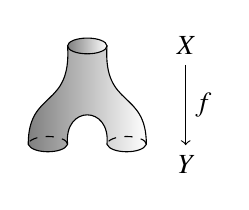
\begin{tikzpicture}[scale=.5]
    \comultc
    \node (Y) at (2.5,-.5) {$Y$};
    \node at (2.5,2.5) {$X$}
      edge [->] node [right] {$f$} (Y);
  \end{tikzpicture}
  $\qquad ~ \qquad$
  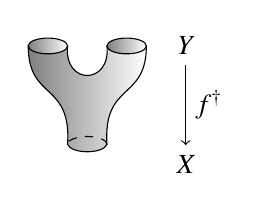
\begin{tikzpicture}[scale=.5]
    \multc
    \node (X) at (2.5,-.5) {$X$};
    \node at (2.5,2.5) {$Y$}
      edge [->] node [right] {$f^{\dagger}$} (X);
  \end{tikzpicture}
\end{center}
In applications to physics, this dagger operation amounts to
`switching the future and the past'.
\end{itemize}

In all the dagger categories above, the dagger structure interacts in a nice way with the monoidal structure and also, when it exists, the braiding.  One can write a list of axioms characterizing how this works \cite{Abramsky,AC,Selinger}.  So, it seems that the ability to `reverse' morphisms is another way in which categories of a quantum flavor differ from the category of sets and functions. This has important implications for the foundations of quantum theory 
\cite{B4} and also for topological quantum field theory \cite{HDATQFT}, where dagger categories seem to be part of larger story involving
`$n$-categories with duals' \cite{HDA4}.  However, this story is still poorly understood --- there is much more work to be done.

\section{Logic}
\label{logic}
\EnableBpAbbreviations 

\subsection{Background}
\label{logic_overview}

Symmetric monoidal closed categories show up not only in physics and topology, but also in logic.  We would like to explain how. To set the stage, it seems worthwhile to sketch a few ideas from
20th-century logic.  

Modern logicians study many systems of reasoning beside ordinary classical logic.  Of course, even classical logic comes in various degrees of strength.  First there is the `propositional calculus', which allows us to reason with abstract propositions 
$X, Y, Z, \dots$ and these logical connectives:
\[  
\begin{array}{cc}
\text{and}        & \wedge   \\
\text{or}         & \vee  \\
\text{implies}    & \Rightarrow \\
\text{not}        & \neg  \\
\text{true}       & \top     \\
\text{false}      & \bot
\end{array}
\]
Then there is the `predicate calculus', which also allows variables like $x,y,z, \dots$, predicates like 
$P(x)$ and $Q(x,y,z)$, and the symbols `for all' ($\forall$) 
and `there exists' ($\exists$), which allow us to quantify over variables. There are also higher-order systems that allow us to quantify over predicates, and so on.  To keep things simple, we mainly confine ourselves to the propositional calculus in what follows.  But even here, there are many alternatives to the `classical' version!

The most-studied of these alternative systems are {\it weaker} 
than classical logic: they make it harder or even impossible to prove things we normally take for granted.  One reason is that some logicians deny that certain familiar principles are actually valid.  But there are also subtler reasons.   One is that studying systems with rules of lesser strength allows for a fine-grained study of precisely which methods of reasoning are needed to prove which results.  Another reason --- the one that concerns us most here --- 
is that dropping familiar rules and then adding them back in one at at time sheds light on the connection between logic and category theory.

For example, around 1907 Brouwer \cite{Heyting} began advocating
`intuitionism'.  As part of this, he raised doubts about the law of excluded middle, which amounts to a rule saying that from $\neg \neg X$ 
we can deduce $X$.  One problem with this principle is that proofs using it are not `constructive'.   For example, we may prove by contradiction that some equation has a solution, but still have no clue how to construct the solution.   For Brouwer, this meant the principle was invalid.

Anyone who feels the law of excluded middle is invalid is duty-bound to study intuitionistic logic.  But, there is another reason for studying this system.  Namely: we do not really {\it lose} anything by dropping the law of excluded middle!  Instead, we {\em gain} a fine-grained distinction: the distinction between a direct proof of $X$ and a proof by contradiction, which yields merely $\neg \neg X$. If we do not care about this distinction we are free to ignore it, but there is no harm in having it around.  

In the 1930's, this idea was made precise by G\"odel \cite{Goedel} and Gentzen \cite{Gentzen}.  They showed that we can embed classical logic in intuitionistic logic.  In fact, they found a map sending any formula $X$ of the propositional calculus to a new formula $X^\circ$, such that $X$ is provable classically if and only if $X^\circ$ is provable intuitionistically.  (More impressively, this map also works for the predicate calculus.)

Later, yet another reason for being interested in intuitionistic logic became apparent: its connection to category theory.  In its very simplest form, this connection works as follows.  Suppose we have a set of propositions $X, Y, Z, \dots$ obeying the laws of the intuitionistic propositional calculus.  We can create a category
$C$ where these propositions are objects and there is at most one morphism from any object $X$ to any object $Y$: a single morphism when $X$ implies $Y$, and none otherwise!  

A category with at most one morphism from any object to any other is called a {\bf preorder}.  In the propositional calculus, we often treat two propositions as equal when they both imply each other. If we do this, we get a special sort of preorder: one where isomorphic objects are automatically equal.  This special sort of preorder is called a {\bf partially ordered set}, or {\bf poset}
for short.  Posets abound in logic, precisely because they offer a simple framework for understanding implication.  

If we start from a set of propositions obeying the intuitionistic propositional calculus, the resulting category $C$ is better than a mere poset.  It is also cartesian, with $X \wedge Y$ as the product of $X$ and $Y$, and $\top$ as the terminal object!  To see this, note that any proposition $Q$ has a unique morphism to $X \wedge Y$ whenever it has morphisms to $X$ and to $Y$.  This is simply a fancy way of saying that $Q$ implies $X \wedge Y$ when it implies $X$ and implies $Y$. It is also easy to see that $\top$ is terminal: anything implies the truth.  

Even better, the category $C$ is cartesian closed, with 
$ X \Rightarrow Y$ as the internal hom.  The reason is that 
\[  X \wedge Y \; \text{implies}\; Z \quad \text{iff} \quad Y 
\; \text{implies} \; X \Rightarrow Z .\]
This automatically yields the basic property of the internal hom:
\[ \hom(X\tensor Y, Z) \cong \hom(Y,X \lhom Z)  . \]
Indeed, if the reader is puzzled by the difference between 
`$X$ implies $Y$' and $X \Rightarrow Y$, we can now explain this more clearly: the former involves the homset $\hom(X,Y)$ 
(which has one element when $X$ implies $Y$ and none otherwise), while the latter is the internal hom, an object in $C$.

So, $C$ is a cartesian closed poset.  But, it also has one more nice property, thanks to the presence of $\vee$ and $\bot$
We have seen that $\wedge$ and $\top$ make the category $C$ cartesian; 
$\vee$ and $\bot$ satisfy exactly analogous rules, but with the implications turned around, so they make $C^\op$ cartesian.  

And that is all!  In particular, negation gives nothing more, since we can define $\neg X$ to be $X \Rightarrow \bot$, and all its intuitionistically valid properties then follow.  So, the kind of category we get from the intuitionistic propositional calculus by taking propositions as objects and implications as morphisms is precisely a {\bf Heyting algebra}: a cartesian closed poset $C$ such that $C^\op$ is also cartesian.

Heyting, a student of Brouwer, introduced Heyting algebras in intuitionistic logic before categories were even invented. So, he used very different language to define them.   But, the category-theoretic approach to Heyting algebras illustrates the connection between cartesian closed categories and logic. It also gives more evidence that dropping the law of excluded middle is an interesting thing to try.

Since we have explained the basics of cartesian closed categories, but not said what happens when the {\it opposite} of such a category is {\it also} cartesian, in the sections to come we will take a drastic step and limit our discussion of logic even further. We will neglect $\vee$ and $\bot$, and concentrate only on the fragment of the propositional calculus involving $\wedge$, $\top$ and 
$\Rightarrow$.  

Even here, it turns out, there are interesting things to say --- and interesting ways to modify the usual rules.  This will be the main subject of the sections to come.  But to set the stage, we need to say a bit about proof theory.

Proof theory is the branch of mathematical logic that treats proofs as mathematical entities worthy of study in their own right. It lets us dig deeper into the propositional calculus by studying not merely {\it whether or not} some assumption $X$ implies some conclusion $Y$, but the whole {\it set of proofs} leading from $X$ to 
$Y$.  This amounts to studying not just posets (or preorders), but categories that allow many morphisms from one object to another.

In Hilbert's approach to proof, there were many axioms and just one rule to deduce new theorems: {\em modus ponens}, which says that from $X$ 
and `$X$ implies $Y$' we can deduce $Y$.  Most of modern proof theory focuses on another approach, the `sequent calculus', due to Gentzen \cite{Gentzen}.  In this approach there are few axioms but many inference rules.  

An excellent introduction to the sequent calculus is the book 
{\it Proofs and Types} by Girard, Lafont and Taylor, freely available online \cite{GLT}.   Here we shall content ourselves with some sketchy remarks.  A `sequent' is something like this:
\[          X_1, \dots, X_m \lHom Y_1, \dots , Y_n  \]
where $X_i$ and $Y_i$ are propositions.  We read this sequent as saying that {\em all} the propositions $X_i$, taken together, can be used to prove at least {\em one} of the propositions $Y_i$.  This strange-sounding convention gives the sequent calculus a nice symmetry, as we shall soon see.

In the sequent calculus, an `inference rule' is something that produces new sequents from old.  For example, here is the
{\bf left weakening} rule:
\begin{center}
\AXC{$X_1, \dots, X_m \lHom Y_1, \dots, Y_n$} 
\UIC{$X_1, \dots , X_m, A \lHom Y_1, \dots, Y_n$} \DP 
\end{center}
This says that from the sequent above the line we can get the sequent below the line: we can throw in the extra assumption $A$ without harm.  Thanks to the strange-sounding convention we mentioned, this rule has a mirror-image version called {\bf right weakening}:
\begin{center}
\AXC{$X_1, \dots, X_m \lHom Y_1, \dots, Y_n$} 
\UIC{$X_1, \dots , X_m  \lHom Y_1, \dots, Y_n, A$} \DP 
\end{center}
In fact, Gentzen's whole setup has this mirror symmetry!
For example, his rule called {\bf left contraction}:
\begin{center}
\AXC{$X_1, \dots, X_m, A, A \lHom Y_1, \dots, Y_n$} 
\UIC{$X_1, \dots , X_m, A \lHom Y_1, \dots, Y_n$} \DP 
\end{center}
has a mirror partner called {\bf right contraction}:
\begin{center}
\AXC{$X_1, \dots, X_m \lHom Y_1, \dots, Y_n, A, A$} 
\UIC{$X_1, \dots , X_m \lHom Y_1, \dots, Y_n, A$} \DP 
\end{center}
Similarly, this rule for `and'
\begin{center}
\AXC{$X_1, \dots, X_m, A \lHom Y_1, \dots, Y_n$} 
\UIC{$X_1, \dots , X_m, A \wedge B \lHom Y_1, \dots, Y_n$} \DP 
\end{center}
has a mirror partner for `or':
\begin{center}
\AXC{$X_1, \dots, X_m \lHom Y_1, \dots, Y_n, A$} 
\UIC{$X_1, \dots , X_m  \lHom Y_1, \dots, Y_n, A \vee B$} \DP 
\end{center}
Logicians now realize that this mirror symmetry can be understood in terms of the duality between a category and its opposite.  

Gentzen used sequents to write inference rules for the classical propositional calculus, and also the classical predicate calculus. Now, in these forms of logic we have
\[          X_1, \dots, X_m \lHom Y_1, \dots, Y_n  \]
if and only if we have
\[ X_1 \wedge \cdots \wedge X_m \lHom Y_1 \vee \cdots \vee Y_n  .\]
So, why did Gentzen use sequents with a {\it list} of propositions on each side of the $\lHom$ symbol, instead just a single proposition?
The reason is that this let him use only inference rules having the 
`subformula property'.  This says that every proposition in the sequent above the line appears as part of some proposition in the sequent below the line.  So, a proof built from such inference rules becomes a `tree' where all the propositions further up the tree are subformulas of those below.

This idea has powerful consequences.  For example, in 1936 Gentzen was able prove the consistency of Peano's axioms of arithmetic!
His proof essentially used induction on trees  (Readers familiar with G\"odel's second incompleteness theorem should be reassured that this sort of induction cannot itself be carried out in Peano arithmetic.)

The most famous rule {\em lacking} the subformula property is the `cut rule':
\begin{center}
\AXC{$X_1, \dots, X_m \lHom Y_1, \dots, Y_k, A$} 
\AXC{$X_{m+1}, \dots, X_n, A \lHom Y_{k+1}, \dots, Y_{\ell}$} 
\BIC{$X_1, \dots , X_n \lHom Y_1, \dots, Y_\ell$} \DP 
\end{center}
From the two sequents on top, the cut rule gives us the sequent below.  Note that the intermediate step $A$ does not appear in the sequent below.  It is `cut out'.  So, the cut rule lacks the subformula property.  But, one of Gentzen's great achievements was to show that any proof in the classical propositional (or even predicate) calculus that can be done {\it with} the cut rule can also be done {\it without}
it.  This is called `cut elimination'.  

Gentzen also wrote down inference rules suitable for the intuitionistic propositional and predicate calculi.  These rules lack the mirror symmetry of the classical case.  But in the 1980s, this symmetry was restored by Girard's invention of `linear logic' \cite{Girard1}.  

Linear logic lets us keep track of how many times we use a given premise to reach a given conclusion.   To accomplish this, Girard introduced some new logical connectives!   For starters, he introduced `linear' connectives called $\tensor$ and $\lhom$, and a logical constant called $I$.  These act a bit like $\wedge$, $\Rightarrow$ and $\top$.  However, they satisfy rules corresponding to a symmetric monoidal category instead of a cartesian closed category.  In particular, from $X$ we can prove neither $X \tensor X$ 
nor $I$.  So, we cannot freely `duplicate' and `delete' propositions using these new connectives.   This is reflected in the fact that linear logic drops Gentzen's contraction and weakening rules. 

By itself, this might seem unbearably restrictive.  However, Girard 
{\it also} kept the connectives $\wedge$, $\Rightarrow$ and $\top$ in his system, still satisfying the usual rules.  And, he introduced an operation called the `exponential', $!$, which takes a proposition $X$ 
and turns it into an `arbitrary stock of copies of $X$'.  So, for example, from $!X$ we can prove $I$, and $X$, and $X \tensor X$, and 
$X \tensor X \tensor X$, and so on.  

Full-fledged linear logic has even more connectives than we have described here.  It seems baroque and peculiar at first glance.   It also comes in both classical and intuitionistic versions!  But, {\it just as classical logic can be embedded in intuitionistic logic, intuitionistic logic can be embedded in intuitionistic linear logic} \cite{Girard1}.  So, we do not lose any deductive power.  Instead, we gain the ability to make even more fine-grained distinctions.

In what follows, we discuss the fragment of intuitionistic linear logic involving only $\tensor, \lhom$ and $I$.  This is called
`multiplicative intuitionistic linear logic' \cite{Hasegawa,Schalk}. It turns out to be the system of logic suitable for closed symmetric monoidal categories --- nothing more or less.

\subsection{Proofs as Morphisms}
\label{proof_theory}

In Section \ref{physics_topology} we described categories with various amounts of extra structure, starting from categories pure and simple, and working our way up to monoidal categories, braided monoidal categories, symmetric monoidal categories, and so on.  Our treatment only scratched the surface of an enormously rich taxonomy.  In fact, each kind of category with extra structure corresponds to a system of logic with its own inference rules!

To see this, we will think of {\em propositions} as {\em objects} in some category, and {\em proofs} as giving {\em morphisms}.  Suppose
$X$ and $Y$ are propositions.  Then, we can think of a proof starting from the assumption $X$ and leading to the conclusion $Y$ as giving a morphism $f \maps X \to Y$.  (In Section \ref{theories} we shall see that a morphism is actually an equivalence class of proofs --- but for now let us gloss over this issue.)

Let us write $X \lHom Y$ when, starting from the assumption 
$X$, there is a proof leading to the conclusion $Y$.   An inference rule is a way to get new proofs from old.  For example, in almost every system of logic, if there is a proof leading from $X$ to $Y$, and a proof leading from $Y$ to $Z$, then there is a proof leading from $X$ 
to $Z$.  We write this inference rule as follows:

\begin{center}
\AXC{$X \lHom Y$} \AXC{$Y \lHom Z$} \BIC{$X \lHom Z$} \DP 
\end{center}

\noindent We can call this {\bf cut rule}, since it lets us `cut out'
the intermediate step $Y$.   It is a special case of Gentzen's cut rule, mentioned in the previous section.  It should remind us of composition of morphisms in a category: if we have a morphism 
$f \maps X \to Y$ and a morphism $g \maps Y \to Z$, we get a morphism 
$gf \maps X \to Z$.

Also, in almost every system of logic there is a proof leading from $X$ to $X$.  We can write this as an inference rule that starts with {\em nothing} and concludes the existence of a proof of $X$ from $X$:

\begin{center}
\AXC{} \UIC{$X\lHom X$} \DP 
\end{center}

\noindent This rule should remind us of how every object in category has an identity morphism: for any object $X$, we automatically get a morphism $1_X \maps X \to X$.  Indeed, this rule is sometimes called the {\bf identity rule}.

If we pursue this line of thought, we can take the definition of a closed symmetric monoidal category and extract a collection of inference rules.  Each rule is a way to get new morphisms from old in a closed symmetric monoidal category.  There are various superficially different but ultimately equivalent ways to list these rules.  Here is one:

\cent{\begin{tabular}{ccc}
     \AXC{} \UIC{$X\lHom X$} \DP {\scriptsize ($\id$)} &\hbox{\qquad}&
     \AXC{$X \lHom Y$} \AXC{$Y \lHom Z$} \BIC{$X \lHom Z$} \DP 
{\scriptsize ($\cut$)} \\ \\
     \AXC{$W \lHom X$} \AXC{$Y \lHom Z$} \BIC{$W \tensor Y \lHom X \tensor Z$} \DP {\scriptsize ($\tensor$)}  &&
     \AXC{$W \lHom (X \tensor Y) \tensor Z$} \doubleLine \UIC{$W \lHom X \tensor (Y \tensor Z)$} \DP 
{\scriptsize ({\rm a})} \\ \\
     \AXC{$X \lHom I \tensor Y$} \doubleLine \UIC{$X \lHom Y$} \DP 
{\scriptsize ({\rm l})} &&
     \AXC{$X \lHom Y \tensor I$} \doubleLine \UIC{$X \lHom Y$} \DP 
{\scriptsize ({\rm r})} \\  \\  
     \AXC{$W \lHom X \tensor Y$} \doubleLine \UIC{$W \lHom Y \tensor X$} \DP 
{\scriptsize ({\rm b})} &&
     \AXC{$X \tensor Y \lHom Z$} \doubleLine \UIC{$Y \lHom X \lhom Z$} \DP 
{\scriptsize ({\rm c})} 
\end{tabular}}

\noindent Double lines mean that the inverse rule also holds.  We have given each rule a name, written to the right in parentheses. As already explained, rules ($\id$) and 
($\cut$) come from the presence of identity morphisms and composition in any category.  Rules ($\tensor$), 
(a), (l), and (r) come from tensoring, the associator, and the left and right unitors in a monoidal category.  Rule (b) comes from the braiding in a braided monoidal category, and rule (c) 
comes from currying in a closed monoidal category.

Now for the big question: {\it what does all this mean in terms of logic?}
These rules describe a small fragment of the propositional calculus. To see this, we should read the connective $\tensor$ as `and', the connective $\lhom$ as `implies', and the proposition $I$ as `true'.  

In this interpretation, rule (c) says we can turn a proof leading from the assumption `$Y$ and $X$' to the conclusion $Z$ into a proof leading from $X$ to `$Y$ implies $Z$'.  It also says we can do the reverse. This is true in classical, intuitionistic and linear logic, and so are all the other rules.  Rules (a) and (b) say that `and' is associative and commutative. Rule (l) says that any proof leading from the assumption $X$ to the conclusion `true and $Y$' can be converted to a proof leading from 
$X$ to $Y$, and vice versa.  Rule (r) is similar.

What do we do with these rules?  We use them to build `deductions'. Here is an easy example:
\begin{center}
\AXC{}
\RightLabel{\scriptsize ($\id$)} 
\UIC{$X \lhom Y \lHom X \lhom Y$} 
\RightLabel{\scriptsize (${\rm c}^{-1})$} 
\UIC{$X \tensor (X \lhom Y) \lHom Y$} 
\DP
\end{center}
First we use the identity rule, and then the inverse of the currying rule.  At the end, we obtain
$$   X \tensor (X \lhom Y) \lHom Y . $$
This should remind us of the evaluation morphisms we have in a closed monoidal category:
$$\ev_{X,Y} \maps X \tensor (X \lhom Y) \to Y. $$
In terms of logic, the point is that we can prove 
$Y$ from $X$ and `$X$ implies $Y$'.  This fact comes in handy so often that we may wish to abbreviate the above deduction as an extra inference rule --- a rule derived from our basic list:
\begin{center}
\AXC{}
\RightLabel{\scriptsize (ev)} 
\UIC{$X \tensor (X \lhom Y) \lHom Y$} 
\DP
\end{center}
This rule is called {\bf modus ponens}.

In general, a deduction is a tree built from inference rules. Branches arise when we use the ($\circ$) or ($\tensor$) rules. Here is an example:
\begin{center}
\AXC{}
\RightLabel{\scriptsize (i)}
\UIC{$(A \tensor B) \tensor C \lHom
(A \tensor B) \tensor C$}
\RightLabel{\scriptsize (a)} 
\UIC{$(A \tensor B) \tensor C \lHom A \tensor (B \tensor C)$}
\AXC{$A \tensor (B \tensor C) \lHom D$} 
\RightLabel{\scriptsize ($\circ$)}
\BIC{$(A \tensor B) \tensor C \lHom D$}
\DP
\end{center}
Again we can abbreviate this deduction as a derived rule. In fact, this rule is reversible:
\begin{center}
\AXC{$A \tensor (B \tensor C) \lHom D$} 
\RightLabel{\scriptsize ($\alpha$)} 
\doubleLine
\UIC{$(A \tensor B) \tensor C \lHom D$}
\DP
\end{center}

For a more substantial example, suppose we want to show
$$  (X \lhom Y) \tensor (Y \lhom Z) \lHom X \lhom Z  . $$
The deduction leading to this will not even fit on the page unless we use our abbreviations: 
\begin{center}
\AXC{}
\RightLabel{\scriptsize (ev)}
\UIC{$X \tensor (X \lhom Y) \lHom Y$}
\AXC{}
\RightLabel{\scriptsize ($\id$)}
\UIC{$Y \lhom Z \lHom Y \lhom Z$}
\RightLabel{\scriptsize ($\tensor$)}
\BIC{$(X \tensor (X \lhom Y)) \tensor (Y \lhom Z) \lHom Y \tensor (Y \lhom Z)$}
\AXC{}
\RightLabel{\scriptsize (ev)}
\UIC{$Y \tensor (Y \lhom Z) \lHom Z$}
\RightLabel{\scriptsize ($\circ$)}
\BIC{$(X \tensor (X \lhom Y)) \tensor (Y \lhom Z) \lHom Z$}
\RightLabel{\scriptsize ($\alpha^{-1}$)}
\UIC{$X \tensor ((X \lhom Y) \tensor (Y \lhom Z)) \lHom Z$}
\RightLabel{\scriptsize (c)}
\UIC{$(X \lhom Y) \tensor (Y \lhom Z) \lHom X \lhom Z$}
\DP
\end{center}
Since each of the rules used in this deduction came from a way to get new morphisms from old in a closed monoidal category (we never used the braiding), it follows that in every such category we have 
{\bf internal composition} morphisms:
\[ \bullet_{X,Y,Z}\, \maps (X \lhom Y) \tensor (Y \lhom Z) \to X \lhom Z . \]
These play the same role for the internal hom that ordinary composition
\[  \circ \maps \hom(X,Y) \times \hom(Y,Z) \to \hom(X,Z)  \]
plays for the ordinary hom.

We can go ahead making further deductions in this system of logic, but the really interesting thing is what it omits. For starters, it omits the connective `or' and the proposition `false'.  It also omits two inference rules we normally take for granted --- namely, {\bf contraction}: 

\begin{center}
\AXC{$X \lHom Y$} \RightLabel{\scriptsize $(\Delta)$} 
\UIC{$X \lHom Y \tensor Y$}\DP 
\end{center}

\noindent and {\bf weakening}:

\begin{center}
\AXC{$X \lHom Y$} \RightLabel{\scriptsize $(!)$} \UIC{$X \lHom I$} \DP
\end{center}

\noindent which are closely related to duplication and deletion in a cartesian category.  Omitting these rules is a distinctive feature of linear logic \cite{Girard1}.  The word `linear' should remind us of the category $\Hilb$.  As noted in Section
\ref{monoidal}, this category with its usual tensor product is noncartesian, so it does not permit duplication and deletion. But, what does omitting these rules mean {\it in terms of logic?}

Ordinary logic deals with propositions, so we have been thinking of the above system of logic in the same way.  Linear logic deals not just with propositions, but also other resources --- for example, physical things!  Unlike propositions in ordinary logic, we typically can't duplicate or delete these other resources.  In classical logic, if we know that a proposition $X$ is true, we can use $X$ as many or as few times as we like when trying to prove some proposition $Y$.   But if we have a cup of milk, we can't use it to make cake and then use it again to make butter.  Nor can we make it disappear without a trace: even if we pour it down the drain, it must go somewhere.

In fact, these ideas are familiar in chemistry.  Consider the following resources:
\[
\begin{array}{ccl}
          \H_2  &=& \text{one molecule of hydrogen} \\
          \O_2  &=& \text{one molecule of oxygen} \\
          \H_2\O &=& \text{one molecule of water} \\
\end{array}
\]
We can burn hydrogen, combining one molecule of oxygen with two of hydrogen to obtain two molecules of water. A category theorist might describe this reaction as a morphism:
\[        f \maps \O_2 \tensor (\H_2 \tensor \H_2) \to 
                  \H_2\O \tensor \H_2\O .  \]
A linear logician might write:
\[        \O_2 \tensor (\H_2 \tensor \H_2) \lHom \H_2\O \tensor \H_2\O    \]
to indicate the existence of such a morphism.  But, we cannot duplicate or delete molecules, so for example
\[         \H_2 \not{\lHom} \H_2 \tensor \H_2 \]
and
\[         \H_2 \not{\lHom} I \]
where $I$ is the unit for the tensor product: not iodine, but
`no molecules at all'.

In short, ordinary chemical reactions are morphisms in a symmetric monoidal category where objects are collections of molecules.  As chemists normally conceive of it, this category is not closed.  So, it obeys an even more limited system of logic than the one we have been discussing, a system lacking the connective $\lhom$. To get a closed category --- in fact a compact one --- we need to remember one of the great discoveries of 20th-century physics: {\em antimatter}.  This lets us define 
$Y \lhom Z$ to be `anti-$Y$ and $Z$':
\[         Y \lhom Z = Y^* \tensor Z . \]
Then the currying rule holds:

\begin{center}
 \AXC{$Y \tensor X \lHom Z$} \doubleLine \UIC{$X \lHom Y^\ast \tensor Z$} \DP 
\end{center}
 
\noindent Most chemists don't think about antimatter very often
--- but particle physicists do.  They don't use the notation of linear logic or category theory, but they know perfectly well that since a neutrino and a neutron can collide and turn into a proton and an electron:
\[   \nu \tensor n \lHom p \tensor e , \]
then a neutron can turn into an antineutrino together with a proton and an electron:
\[   n \lHom \nu^* \tensor (p \tensor e) . \]
This is an instance of the currying rule, rule (c).

\subsection{Logical Theories from Categories}
\label{theories}

We have sketched how different systems of logic naturally arise from different types of categories.  To illustrate this idea, we introduced a system of logic with inference rules coming from ways to get new morphisms from old in a {\it closed symmetric monoidal category}.  One could substitute many other types of categories here, and get other systems of logic.  

To tighten the connection between proof theory and category theory, we shall now describe a recipe to get a logical theory from any closed symmetric monoidal category.  For this, we shall now use 
$X\lHom Y$ to denote the {\em set} of proofs --- or actually, equivalence classes of proofs --- leading from the assumption $X$ 
to the conclusion $Y$.  This is a change of viewpoint.  Previously we would write $X \lHom Y$ when this set of proofs was nonempty;
otherwise we would write $X \not{\lHom} Y$.  The advantage of treating $X \lHom Y$ as a set is that this set is precisely what a category theorist would call $\hom(X,Y)$: a homset in a category.

If we let $X \lHom Y$ stand for a homset, an inference rule becomes a function from a product of homsets to a single homset. For example, the cut rule

\begin{center}
\AXC{$X \lHom Y$} \AXC{$Y \lHom Z$} 
\RightLabel{\scriptsize ($\circ$)} 
\BIC{$X \lHom Z$} \DP 
\end{center}

\noindent becomes another way of talking about the composition function
$$  \circ_{X,Y,Z} \maps \hom(X,Y) \times \hom(Y,Z) \to \hom(X,Z), $$
while the identity rule

\begin{center}
\AXC{} 
\RightLabel{\scriptsize ($\id$)}
\UIC{$X\lHom X$} \DP 
\end{center}

\noindent becomes another way of talking about the function
$$  \id_X \maps 1 \to \hom(X,X) $$
that sends the single element of the set 1 to the identity morphism of $X$.  (Note: the set 1 is a {\em zero-fold} product of homsets.)

Next, if we let inference rules be certain functions from products of homsets to homsets, deductions become more complicated functions of the same sort built from these basic ones.  For example, this deduction:
\begin{center}
\AXC{} 
\RightLabel{\scriptsize ($\id$)} 
\UIC{$X\tensor I \lHom X \tensor I$} 
\RightLabel{\scriptsize (r)}   
\UIC{$X\tensor I \lHom X$}
\AXC{}
\RightLabel{\scriptsize ($\id$)} 
\UIC{$Y \lHom Y$}
\RightLabel{\scriptsize ($\tensor$)} 
\BIC{$(X \tensor I) \tensor Y \lHom X \tensor Y$}
\DP
\end{center}
specifies a function from $1$ to
$\hom((X \tensor I) \tensor Y, X \tensor Y)$, built from the basic functions indicated by the labels at each step. This deduction: 
\begin{center}
                                   \AXC{} 
    \RightLabel{\scriptsize ($\id$)} \UIC{$(X \tensor I) \tensor Y \lHom (X \tensor I) \tensor Y$} 
    \RightLabel{\scriptsize (a)}   \UIC{$(X \tensor I) \tensor Y \lHom X \tensor (I \tensor Y)$}
                                   \AXC{} 
    \RightLabel{\scriptsize ($\id$)} \UIC{$I \tensor Y \lHom I \tensor Y$} 
    \RightLabel{\scriptsize (r)}   \UIC{$I \tensor Y \lHom Y$}
                                   \AXC{} 
    \RightLabel{\scriptsize ($\id$)} \UIC{$X \lHom X$} 
    \RightLabel{\scriptsize ($\tensor$)} \BIC{$X \tensor (I \tensor Y) \lHom X \tensor Y$}
    \RightLabel{\scriptsize ($\circ$)} \BIC{$(X \tensor I) \tensor Y \lHom X \tensor Y$}
    \DP
\end{center}
gives another function from 1 to 
$\hom((X \tensor I) \tensor Y, X \tensor Y)$.

If we think of deductions as giving functions this way, the question arises when two such functions are equal.  In the example just mentioned, the triangle equation in the definition of monoidal category
(Definition \ref{mon.cat}): 
\di{
\node{(X\tensor I)\tensor Y}\arrow[2]{e,t}{a_{X,I,Y}}\arrow{se,b}{r_X\tensor 1_Y}
\node[2]{X\tensor(I\tensor Y)}\arrow{sw,b}{1_X\tensor l_Y}\\
\node[2]{X\tensor Y}
}
says these two functions {\em are} equal.  Indeed, the triangle equation is precisely the statement that these two functions agree!  (We leave this as an exercise for the reader.)

So: even though two deductions may look quite different, they may give the same function from a product of homsets to a homset if we demand that these are homsets in a closed symmetric monoidal category.  This is why we think of $X \lhom Y$ as a set of {\em equivalence classes}
of proofs, rather than proofs: it is forced on us by our desire to use category theory.  We could get around this by using a 2-category with proofs as morphisms and `equivalences between proofs' as 2-morphisms
\cite{Seely}.  This would lead us further to the right in the Periodic Table (Table \ref{periodic_table}).  But let us restrain ourselves and make some definitions formalizing what we have done so far.

From now on we shall call the objects $X,Y, \dots$ 
`propositions', even though we have seen they may represent more general resources.  Also, purely for the sake of brevity, we use the term `proof' to mean `equivalence class of proofs'. The equivalence relation must be coarse enough to make the equations in the following definitions hold:

\begin{definition}
A {\bf closed monoidal theory} consists of the following:
\begin{itemize}
    \item A collection of {\bf propositions}.  The collection must contain a proposition $I$, and if $X$ and $Y$ are propositions, then so are $X \tensor Y$ and $X \lhom Y$. 
    \item For every pair of propositions $X,Y,$ a set $X \lHom Y$ of 
{\bf proofs} leading from $X$ to $Y$.  If $f \in X \lHom Y,$ then we write $f \maps X\to Y$.
     \item Certain functions, written as {\bf inference rules}:
{\rm 
\cent{\begin{tabular}{ccc}
     \AXC{} \UIC{$X\lHom X$} \DP {\scriptsize ($\id$)} &\hbox{\qquad}&
     \AXC{$X \lHom Y$} \AXC{$Y \lHom Z$} \BIC{$X \lHom Z$} \DP 
{\scriptsize ($\cut$)} \\ \\
     \AXC{$W \lHom X$} \AXC{$Y \lHom Z$} \BIC{$W \tensor Y \lHom X \tensor Z$} 
\DP {\scriptsize ($\tensor$)}  &&
     \AXC{$W \lHom (X \tensor Y) \tensor Z$} \doubleLine \UIC{$W \lHom X \tensor (Y \tensor Z)$} \DP 
{\scriptsize ({\rm a})} \\ \\
     \AXC{$X \lHom I \tensor Y$} \doubleLine \UIC{$X \lHom Y$} \DP 
{\scriptsize ({\rm l})} &&
     \AXC{$X \lHom Y \tensor I$} \doubleLine \UIC{$X \lHom Y$} \DP 
{\scriptsize ({\rm r})} \\  \\  
     \AXC{$X \tensor Y \lHom Z$} \doubleLine \UIC{$Y \lHom X \lhom Z$} \DP 
{\scriptsize ({\rm c})} &&
\end{tabular}}
}
A double line means that the function is invertible.  So, for example, for each triple $X,Y,Z$ we have a function 
\[     \circ_{X,Y,Z} \maps (X \lHom Y) \times (Y \lHom Z) \; \to \; 
(X \lHom Z) \]
and a bijection
\[     c_{X,Y,Z} \maps (X \tensor Y \lHom Z) \; \to \; (Y \lHom X \lhom Z) .\]
    \item Certain equations that must be obeyed by the inference rules. The inference rules $(\circ)$ and $(\id)$ must obey equations describing associativity and the left and right unit laws. Rule $(\tensor)$ must obey an equation saying it is a functor. Rules {\rm (a)}, {\rm (l)}, {\rm (r)}, and {\rm (c)} must obey equations saying they are natural transformations. Rules {\rm (a)}, {\rm (l)}, {\rm (r)} and $(\tensor)$ must also obey the triangle and pentagon equations.  
\end{itemize}
\end{definition}

\begin{definition}
A {\bf closed braided monoidal theory} is a closed monoidal theory with this additional inference rule:
{\rm 
\begin{center}
     \AXC{$W \lHom X \tensor Y$} \doubleLine \UIC{$W \lHom Y \tensor X$} \DP 
{\scriptsize (\rm b)} 
\end{center}
}
\noindent We demand that this rule give a natural transformation satisfying the hexagon equations.  
\end{definition}

\begin{definition}
A {\bf closed symmetric monoidal theory} is a closed braided monoidal theory where the rule {\rm (b)} is its own inverse.
\end{definition}

These are just the usual definitions of various kinds of closed category --- monoidal, braided monoidal and symmetric monoidal ---
written in a new style.  This new style lets us \emph{build such categories from logical systems}.  To do this, we take the objects to be propositions and the morphisms to be equivalence classes of proofs, where the equivalence relation is generated by the equations listed in the definitions above.

However, the full advantages of this style only appear when we dig deeper into proof theory, and generalize the expressions we have been considering: 
\[   X \lHom Y \]
to `sequents' like this: 
\[   X_1, \dots, X_n \lHom Y . \]
Loosely, we can think of such a sequent as meaning
\[ X_1 \tensor \cdots \tensor X_n \lHom Y .\]
The advantage of sequents is that they let us use inference rules that
--- except for the cut rule and the identity rule --- have the
`subformula property' mentioned near the end of Section
\ref{logic_overview}.

Formulated in terms of these inference rules, the logic of closed symmetric monoidal categories goes by the name of `multiplicative intuitionistic linear logic', or MILL for short \cite{Hasegawa, Schalk}.  There is a `cut elimination' theorem for MILL, which says that with a suitable choice of other inference rules, the cut rule becomes redundant: any proof that can be done with it can be done without it.  This is remarkable, since the cut rule corresponds to
{\it composition of morphisms} in a category.  One consequence is that in the free symmetric monoidal closed category on any set of objects, the set of morphisms between any two objects is {\it finite}.  There is also a decision procedure to tell when two morphisms are equal. For details, see Trimble's thesis \cite{Trimble} and the papers by Jay
\cite{Jay1990} and Soloviev \cite{Soloviev}.  Also see Kelly and Mac Lane's coherence theorem for closed symmetric monoidal categories
\cite{KM}, and the related theorem for compact symmetric monoidal categories \cite{KellyLaplaza}.

MILL is just one of many closely related systems of logic.  Most include extra features, but some {\it subtract} features. Here are just a few examples:

\begin{itemize}
\item Algebraic theories.   In his famous thesis, Lawvere \cite{Lawvere}
defined an {\bf algebraic theory} to be a cartesian category where every object is an $n$-fold cartesian power $X \times \cdots \times X$ 
($n \ge 0$) of a specific object $X$.  He showed how such categories regarded as logical theories of a simple sort --- the sort that had previously been studied in `universal algebra' \cite{BurrisS}.  This work initiated the categorical approach to logic which we have been sketching here.  Crole's book \cite{Crole} gives a gentle introduction to algebraic theories as well as some richer logical systems. More generally, we can think of any cartesian category as a generalized algebraic theory. 
\item Intuitionistic linear logic (ILL).  ILL
supplements MILL with the operations familiar from intuitionistic logic, as well as an operation $!$ turning any proposition (or resource) $X$ into an `indefinite stock of copies of $X$'.  Again there is a nice category-theoretic interpretation.  Bierman's thesis \cite{BiermanThesis} gives a good overview, including a proof of cut elimination for ILL and a proof of the result, originally due to Girard, that intuitionistic logic can be be embedded in ILL.
\item Linear logic (LL).  For full-fledged linear logic, the online review article by Di Cosmo and Miller \cite{dCM} is a good place to start.  For more, try the original paper by Girard \cite{Girard1} and the book by Troelstra \cite{Troelstra}. Blute and Scott's review article \cite{BS} serves as a Rosetta Stone for linear logic and category theory, and so do the lectures notes by Schalk \cite{Schalk}.  \item Intuitionistic Logic (IL).   Lambek and Scott's classic book \cite{LS} is still an excellent introduction to intuitionistic logic and cartesian closed categories.  The online review article by Moschovakis \cite{Moschovakis} contains many suggestions for further reading.
\end{itemize}

To conclude, let us say precisely what an `inference rule' amounts to in the setup we have described.  We have said it gives a function from a product of homsets to a homset.  While true, this is not the last word on the subject.  After all, instead of treating the propositions appearing in an inference rule as {\it fixed}, we can treat them as
{\it variable}.  Then an inference rule is really a `schema' for getting new proofs from old.  How do we formalize this idea?

First we must realize that $X \lHom Y$ is not just a set: it is a set 
{\em depending in a functorial way} on $X$ and $Y$.   As noted in Definition \ref{hom.functor}, there is a functor, the `hom functor'
$$    \hom \maps C^\op \times C \to \Set, $$ 
sending $(X,Y)$ to the homset $\hom(X,Y) = X \lHom Y$.  To look like logicians, let us write this functor as $\lHom$.

Viewed in this light, most of our inference rules are {\it natural transformations}.  For example, rule (a) is a natural transformation between two functors from $C^\op \times C^3$ to $\Set$, namely the functors 
\[        (W,X,Y,Z) \mapsto W \lHom (X \tensor Y) \tensor Z \]
and 
\[        (W,X,Y,Z) \mapsto W \lHom X \tensor (Y \tensor Z) .\]
This natural transformation turns any proof
\[        f \maps W \to (X \tensor Y) \tensor Z \]
into the proof
\[  a_{X,Y,Z} f \maps W \to X \tensor (Y \tensor Z)  .\]
The fact that this transformation is {\it natural} means that it changes in a systematic way as we vary $W,X,Y$ and $Z$.  The commuting square in the definition of natural transformation, Definition \ref{naturality}, makes this precise.

Rules (l), (r), (b) and (c) give natural transformations in a very similar way.   The $(\tensor)$ rule gives a natural transformation between two functors from $C^\op \times C \times C^\op \times C$ 
to $\Set$, namely
\[       (W,X,Y,Z) \mapsto (W \lHom X) \; \times \; (Y \lHom Z) \]
and 
\[       (W,X,Y,Z) \mapsto W \tensor Y \lHom X \tensor Z .\]
This natural transformation sends any element $(f,g) \in 
\hom(W,X) \times \hom(Y,Z)$ to $f \tensor g$. 

The identity and cut rules are different: they {\it do not} give natural transformations, because the top line of these rules has a different number of variables than the bottom line!
Rule (i) says that for each $X \in C$ there is a function 
\[ \id_X \maps 1 \; \to \; X \lHom X \] 
picking out the identity morphism $1_X.$  
What would it mean for this to be natural in $X$?
Rule $(\circ)$ says that for each triple $X,Y,Z \in C$ there is a function
\[     \circ \maps (X \lHom Y) \; \times \; (Y \lHom Z) \; \to \; X \lHom Z .\] 
What would it mean for this to be natural in $X,Y$ and $Z$? 
The answer to both questions involves a generalization of natural transformations called `dinatural' transformations \cite{MacLane}.

As noted in Definition \ref{naturality}, a natural transformation $\alpha \maps F\Rightarrow G$ between two functors 
$F, G \maps C \to D$ makes certain squares in $D$ commute. If in fact $C=C_1^{\op} \times C_2,$ then we actually obtain commuting cubes in $D.$  Namely, the natural transformation $\alpha$ assigns to each object $(X_1, X_2)$ a morphism $\alpha_{X_1,X_2}$ such that for any morphism $(f_1 \maps Y_1\to X_1, f_2 \maps X_2\to Y_2)$ in $C$, this cube commutes:

\begin{center}
\dgARROWLENGTH=3.75em
\di{
\node[2]{G(Y_1,X_2)}\arrow[2]{e,t,1}{G(1_{Y_1},f_2)}
\node[2]{G(Y_1,Y_2)}\arrow[2]{s,r,1}{G(f_1,1_{Y_2})}
\\
\node{F(Y_1,X_2)}\arrow[2]{s,r,1}{F(f_1,1_{X_2})}\arrow[2]{e,t,1}{F(1_{Y_1},f_2)}\arrow{ne,l}{\alpha_{Y_1,X_2}}
\node{}\arrow{n,r,-}{G(f_1,1_{X_2})}\arrow{s}
\node{F(Y_1,Y_2)}\arrow[2]{s,r,1}{F(f_1,1_{Y_2})}\arrow{ne,l}{\alpha_{Y_1,Y_2}}
\\
\node[2]{G(X_1,X_2)}\arrow{e,t,-}{G(1_{X_1},f_2)}
\node{}\arrow{e}
\node{G(X_1,Y_2)}
\\
\node{F(X_1,X_2)}\arrow[2]{e,t}{F(1_{X_1},f_2)}\arrow{ne,r,3}{\alpha_{X_1,X_2}}
\node[2]{F(X_1,Y_2)}\arrow{ne,r,3}{\alpha_{X_1,Y_2}}
}
\end{center}

If $C_1 = C_2,$ we can choose a single object $X$ and a single morphism $f \maps X\to Y$ and use it in both slots.  As shown in Figure \ref{dinaturalcube}, there are then two paths from one corner of the cube to the antipodal corner that only involve $\alpha$ 
for repeated arguments: that is, $\alpha_{X,X}$ and $\alpha_{Y,Y}$, but not $\alpha_{X,Y}$ or $\alpha_{Y,X}$.   These paths give a commuting hexagon.  

\begin{figure}
\begin{center}
\dgARROWLENGTH=3.75em
\di{
\node[2]{G(Y,X)}
\node[2]{G(Y,Y)}\arrow[2]{s,r}{G(f,1_{Y})}
\\
\node{F(Y,X)}\arrow[2]{s,r}{F(f,1_{X})}\arrow[2]{e,t}{F(1_{Y},f)}
\node{}\arrow{n,!}{}\arrow{s,!}
\node{F(Y,Y)}\arrow{ne,l}{\alpha_{Y,Y}}
\\
\node[2]{G(X,X)}\arrow[2]{e,t}{G(1_{X},f)}
\node{}
\node{G(X,Y)}
\\
\node{F(X,X)}\arrow{ne,r}{\alpha_{X,X}}
\node[2]{F(X,Y)}
}
\caption{A natural transformation between functors 
${F,G\maps C^{\op}\times C \to D}$ gives a commuting cube in 
$D$ for any morphism $f \maps X \to Y$, and there are two paths around the cube that only involve $\alpha$ for repeated arguments.}
\label{dinaturalcube}
\end{center}
\end{figure}

This motivates the following:

\begin{definition}
    A {\bf dinatural transformation} $\alpha \maps F\Rightarrow G$ between
    functors $F,G \maps C^{\op}\times C \to D$ assigns to every object $X$
    in $C$ a morphism $\alpha_X \maps F(X,X) \to G(X,X)$ in $D$ such that
    for every morphism $f \maps X\to Y$ in $C$, the hexagon in Figure
    \ref{dinaturalcube} commutes.
\end{definition}

In the case of the identity rule, this commuting hexagon follows from the fact that the identity morphism is a left and right unit for composition: see Figure \ref{hypcube}.  For the cut rule, this commuting hexagon says that composition is associative:
see Figure \ref{cutcube}.

{
So, in general, the sort of logical theory we are discussing involves:
\begin{itemize}
\item A \emph{category} $C$ of propositions and proofs.
\item A \emph{functor} $\lHom \maps C^\op \times C \to \Set$
sending any pair of propositions to the set of proofs leading from one to the other.
\item A set of \emph{dinatural transformations} describing inference rules.
\end{itemize}
}

\begin{figure}
\dgARROWLENGTH=3.75em
\di{
\node[4]{\begin{array}{c}Y\lHom Y\\1_Y\end{array}}
\arrow[2]{s,r}{- \circ f}
\\
\node{\begin{array}{c} 1 \\ \bullet \end{array}}\arrow[2]{s,l}{1_{1}}\arrow[2]{e,t}{1_{1}}
\node{}\arrow{n,!}
\node{\begin{array}{c} 1 \\ \bullet \end{array}}\arrow{ne,l}{\id_Y}
\\
\node[2]{\begin{array}{c}X\lHom X\\1_X\end{array}}\arrow[2]{e,t}{f \circ -}
\node{}
\node{\begin{array}{c}X \lHom Y\\f \circ 1_X = 1_Y \circ f\end{array}}
\\
\node{\begin{array}{c} 1 \\ \bullet \end{array}}\arrow{ne,r}{\id_X}
}
\caption{Dinaturality of the (i) rule, where $f\maps X\to Y$.  Here
$\bullet \in 1$ denotes the one element of the one-element set.}
\label{hypcube}
\end{figure}

\begin{figure}
\dgARROWLENGTH=3.75em
\di{
\node[4]{\begin{array}{c}X\lHom Z\\h \circ (f \circ g)\end{array}}\arrow[2]{s,r}{1_{X\lHom Z}}
\\
\node{\begin{array}{c}(X\lHom W) \; \times \; (Y\lHom Z)\\(g, h)\end{array}}\arrow[2]{s,l}{(1_{X\lHom W}, - \circ f)}\arrow[2]{e,t}{(f \circ -, 1_{Y\lHom Z})}
\node{}\arrow{n,!}
\node{\begin{array}{c}(X\lHom Y) \; \times \; (Y\lHom Z)\\(f \circ g, h)\end{array}}\arrow{ne,l}{\circ}
\\
\node[2]{\begin{array}{c}X\lHom Z\\(h \circ f) \circ g\end{array}}\arrow[2]{e,t}{1_{X\lHom Z}}
\node{}
\node{\begin{array}{c}X\lHom Z\\(h \circ f) \circ g = h \circ (f \circ g)\end{array}}
\\
\node{\begin{array}{c}(X\lHom W) \; \times \; (W\lHom Z)\\(g, h \circ f)\end{array}}\arrow{ne,r}{\circ}
}
\caption{Dinaturality of the cut rule, where 
${f\maps W\to Y,}$ ${g\maps X\to W,}$ ${h\maps Y\to Z.}$
}
\label{cutcube}
\end{figure}

\section{Computation}
\label{computation}

\subsection{Background}
\label{computation_overview}

In the 1930s, while Turing was developing what are now called `Turing machines' as a model for computation, Church and his student Kleene were developing a different model, called the `lambda calculus'
\cite{Church, Kleene}.  While a Turing machine can be seen as an idealized, simplified model of computer {\it hardware}, the lambda calculus is more like a simple model of {\it software}.

By now there are many careful treatments of the lambda calculus in the literature, from Barendregt's magisterial tome \cite{Barendregt}
to the classic category-theoretic treatment of Lambek and Scott
\cite{LS}, to Hindley and Seldin's user-friendly introduction 
\cite{HS} and Selinger's elegant free online notes \cite{Selinger2}.  So, we shall content ourselves with a quick sketch.

Poetically speaking, the lambda calculus describes a universe where everything is a program and everything is data: {\it programs are data}.  More prosaically, everything is a `$\lambda$-term', or `term'
for short.  These are defined inductively:
\begin{itemize}
\item {\bf Variables:}
there is a countable set of `variables' $x, y, z, \dots$
which are all terms. 
\item {\bf Application:}
if $f$ and $t$ are terms, we can `apply' $f$
to $t$ and obtain a term $f(t)$.
\item {\bf Lambda-abstraction:} if 
$x$ is a variable and $t$ is a term, there is a term 
$(\lambda x . t)$.
\end{itemize}

Let us explain the meaning of application and lambda-abstraction. Application is simple.  Since `programs are data', we can think of any term either as a program or a piece of data.  Since we can apply programs to data and get new data, we can apply any term $f$ to any other term $t$ and get a new term $f(t)$.

Lambda-abstraction is more interesting.  We think of $(\lambda x.t)$
as the program that, given $x$ as input, returns $t$ as output. For example, consider
\[       (\lambda x. x(x)) . \]
This program takes any program $x$ as input and returns $x(x)$ as output.  In other words, it applies any program to itself. So, we have
\[       (\lambda x . x(x))(s) = s(s) \]
for any term $s$.  

More generally, if we apply $(\lambda x . t)$ to any term $s$, we should get back $t$, but with $s$ substituted for each free occurrence of the variable $x$.  This fact is codified in a rule called {\bf beta reduction}:
\[       (\lambda x.t)(s) = t[s/x] \]
where $t[s/x]$ is the term we get by taking $t$ and substituting $s$
for each free occurrence of $x$.  But beware: this rule is not an equation in the usual mathematical sense.  Instead, it is a `rewrite rule': given the term on the left, we are allowed to rewrite it and get the term on the right.  Starting with a term and repeatedly applying rewrite rules is how we take a program and let it run!

There are two other rewrite rules in the lambda calculus.  If $x$ is a variable and $t$ is a term, the term
\[    (\lambda x . t(x)) \]
stands for the program that, given $x$ as input, returns $t(x)$ as output.  But this is just a fancy way of talking about the program
$t$.  So, the lambda calculus has a rewrite rule called {\bf eta reduction}, saying
\[        (\lambda x . t(x)) = t. \]

The third rewrite rule is {\bf alpha conversion}.  This allows us to replace a bound variable in a term by another variable. For example:
\[        (\lambda x . x(x)) = (\lambda y . y(y))  \]
since $x$ is `bound' in the left-hand expression by its appearance in `$\lambda x$'.   In other words, $x$ is just a dummy variable;
its name is irrelevant, so we can replace it with $y$.  On the other hand,
\[        (\lambda x . y(x)) \ne (\lambda x . z(x)).  \]
We cannot replace the variable $y$ by the variable $z$ here, since this variable is `free', not bound.  Some care must be taken to make the notions of free and bound variables precise, but we shall gloss over this issue, referring the reader to the references above for details.

The lambda calculus is a very simple formalism.  Amazingly, starting from just this, Church and Kleene were able to build up Boolean logic, the natural numbers, the usual operations of arithmetic, and so on. For example, they defined `Church numerals' as follows:
\[  \begin{array}{ccl}
       \overline{0} &=& (\lambda f . (\lambda x . x))          \\
       \overline{1} &=& (\lambda f . (\lambda x . f(x)))   \\
       \overline{2} &=& (\lambda f . (\lambda x . f(f(x))))   \\
       \overline{3} &=& (\lambda f . (\lambda x . f(f(f(x)))))
\end{array}   \]
and so on.  Note that $f$ is a variable above.  Thus, the Church numeral $\overline{n}$ is the program that `takes any program to the
$n$th power': if you give it any program $f$ as input, it returns the program that applies $f$ $n$ times to whatever input $x$ it receives.

To get a feeling for how we can define arithmetic operations on Church numerals, consider
\[          \lambda g . \overline{3}(\overline{2}(g))  . \]
This program takes any program $g$, squares it, and then cubes the result. So, it raises $g$ to the sixth power.  This suggests that
\[       \lambda g . \overline{3}(\overline{2}(g)) = \overline{6} . \]
Indeed this is true.  If we treat the definitions of Church numerals as reversible rewrite rules, then we can start with the left side of the above equation and grind away using rewrite rules until we reach the right side:
\[
\begin{array}{ccll}
 (\lambda g . \overline{3} (\overline{2} (g))
 &=& (\lambda g . \overline{3} ((\lambda f . (\lambda x . f(f(x))))) (g)) 
  & \textrm{def.\ of } \overline{2} \\
 &=& (\lambda g . \overline{3} (\lambda x . g(g(x))))  
  & \textrm{beta} \\
 &=& (\lambda g . (\lambda f . (\lambda x . f(f(f(x))))) 
     (\lambda x . g(g(x)))) 
  & \textrm{def.\ of } \overline{3} \\
 &=& (\lambda g . (\lambda x . (\lambda x . g(g(x)))
     ((\lambda x . g(g(x))) ((\lambda x . g(g(x))) (x))))) 
  & \textrm{beta} \\
 &=& (\lambda g . (\lambda x . (\lambda x. g(g(x)))
     ((\lambda g . g(g(x))) (g(g(x))))))
  & \textrm{beta} \\
 &=& (\lambda g . (\lambda x . (\lambda x . g(g(x))) (g(g(g(g(x))))))) 
  & \textrm{beta} \\
 &=& (\lambda g . (\lambda x . g(g(g(g(g(g(x))))))))  
  & \textrm{beta} \\
 &=& \overline{6} 
   & \textrm{def.\ of } \overline{6} 
\end{array}
\]
If this calculation seems mind-numbing, that is precisely the point:
it resembles the inner workings of a computer.  We see here how the lambda calculus can serve as a programming language, with each step of computation corresponding to a rewrite rule.

Of course, we got the answer $\overline{6}$ because $3 \times 2 = 6$. Generalizing from this example, we can define a program called `times' that multiplies Church numerals:
\[    \Times = (\lambda a . (\lambda b . (\lambda x . a(b(x))))) .\]
For example, 
\[
\Times(\overline{3})(\overline{2}) = \overline{6} .
\]
The enterprising reader can dream up similar programs for the other basic operations of arithmetic.  With more cleverness, Church and Kleene were able to write terms corresponding to more complicated functions.  They eventually came to believe that {\it all} computable functions $f \maps \NN \to \NN$ can be defined in the lambda calculus.

Meanwhile, G\"odel was developing another approach to computability, the theory of `recursive functions'.  Around 1936, Kleene proved that the functions definable in the lambda calculus were the same as G\"odel's recursive functions.  In 1937 Turing described his `Turing machines', and used these to give yet another definition of computable functions.  This definition was later shown to agree with the other two.  Thanks to this and other evidence, it is now widely accepted that the lambda calculus can define {\it any} function that can be computed by {\it any} systematic method.  We say it is `Turing complete'.

After this burst of theoretical work, it took a few decades for programmable computers to actually be built.  It took even longer for computer scientists to profit from Church and Kleene's insights. This began around 1958, when McCarthy invented the programming language Lisp, based on the lambda calculus \cite{McCarthy}. In 1965, an influential paper by Landin \cite{Landin} pointed out a powerful analogy between the lambda calculus and the language ALGOL.    These developments led to a renewed interest in the lambda calculus which continues to this day.  By now, a number of computer languages are explicitly based on ideas from the lambda calculus.  The most famous of these include Lisp, ML and Haskell.  These languages, called `functional programming languages', are beloved by theoretical computer scientists for their conceptual clarity.  In fact, for many years, everyone majoring in computer science at MIT has been required to take an introductory course that involves programming in Scheme, a dialect of Lisp.  The cover of the textbook for this course \cite{Sussman} even has a big $\lambda$ on the cover!

We should admit that languages of a different sort --- `imperative programming languages' --- are more popular among working programmers. Examples include FORTRAN, BASIC, and C.  In imperative programming, a program is a series of instructions that tell the computer what to do. By constrast, in functional programming, a program simply describes a function.  To run the program, we apply it to an input.  So, as in the lambda calculus, `application' is a fundamental operation in functional programming.  If we combine application with lambda abstraction, we obtain a language powerful enough to compute any computable function.  

However, most functional programming languages are more regimented than the original lambda calculus.  As we have seen, in the lambda calculus as originally developed by Church and Kleene, any term can be applied to any other.  In real life, programming involves many kinds of data.  For example, suppose we are writing a program that involves days of the week.  It would not make sense to write 
\[       \Times(\overline{3})(\Tuesday)  \]
because Tuesday is not a number.  We might choose to represent Tuesday by a number in some program, but doubling that number doesn't have a good interpretation: is the first day of the week Sunday or Monday?
Is the week indexed from zero or one?  These are arbitrary choices that affect the result.  We could let the programmer make the choices, but the resulting unstructured framework easily leads to mistakes.  

It is better to treat data as coming in various `types', such as integers, floating-point numbers, alphanumeric strings, and so on. Thus, whenever we introduce a variable in a program, we should make a `type declaration' saying what type it is.  For example, we might write:
\[ \begin{array}{l}

  \Tuesday:\Day
\end{array}
\]
This notation is used in Ada, Pascal and some other languages.  Other notations are also in widespread use.  Then, our system should have a
`type checker' (usually part of the compiler) that complains if we try to apply a program to a piece of data of the wrong type.

Mathematically, this idea is formalized by a more sophisticated version of the lambda calculus: the `typed' lambda calculus, where every term has a type.  This idea is also fundamental to category theory, where every morphism is like a black box with input and output wires of specified types:
\[\begin{pspicture}(0,0)(2,4)
\psset{angleA=-90,angleB=90,ArrowInside=->,arrowscale=2}
\pnode(1,4){A}
\rput(1,2){\ovalnode{B}{$f$}}
\pnode(1,0){C}
\nccurve{A}{B} \nbput{$X$}
\nccurve{B}{C} \nbput{$Y$}
\end{pspicture}\]
and it makes no sense to hook two black boxes together unless the output of the first has the same type as the input of the next:
\begin{center}
    \begin{pspicture}(0,0)(2,6)
    \psset{angleA=-90,angleB=90,ArrowInside=->,arrowscale=2}
    \pnode(1,6){A}
    \rput(1,4){\ovalnode{B2}{$f$}}
    \rput(1,2){\ovalnode{B1}{$g$}}
    \pnode(1,0){C}
    \nccurve{A}{B2} \nbput{$X$}
    \nccurve{B2}{B1} \nbput{$Y$}
    \nccurve{B1}{C} \nbput{$Z$}
    \end{pspicture}
\end{center}

Indeed, there is a deep relation between the typed lambda calculus and cartesian closed categories.  This was discovered by Lambek in 1980
\cite{Lambek}.  Quite roughly speaking, a `typed lambda-theory' is a very simple functional programming language with a specified collection of basic data types from which other more complicated types can be built, and a specified collection of basic terms from which more complicated terms can be built.  The data types of this language are {\it objects} in a cartesian closed category, while the programs ---
that is, terms --- give {\it morphisms!}

Here we are being a bit sloppy.  Recall from Section \ref{theories}
that in logic we can build closed monoidal categories where the morphisms are equivalence classes of proofs.  We need to take equivalence classes for the axioms of a closed monoidal category to hold.  Similarly, to get closed monoidal categories from computer science, we need the morphisms to be equivalence classes of terms. Two terms count as equivalent if they differ by rewrite rules such as beta reduction, eta reduction and alpha conversion.  As we have seen, these rewrites represent the steps whereby a program carries out its computation.  For example, in the original `untyped' lambda calculus, the terms $\Times(\overline{3})(\overline{2})$ and $\overline{6}$
differ by rewrite rules, but they give the same morphism.  So, when we construct a cartesian closed category from a typed lambda-theory, we
{\it neglect the actual process of computation}.  To remedy this we should work with a cartesian closed 2-category which has:
\begin{itemize}
\item types as objects,
\item terms as morphisms,
\item equivalence classes of rewrites as 2-morphisms.
\end{itemize}
For details, see the work of Seely \cite{Seely}, Hilken \cite{Hilken}, and Melli\'es \cite{Mellies}.  Someday this work will be part of the larger $n$-categorical Rosetta Stone mentioned at the end of Section
\ref{symmetric}.

In any event, Lambek showed that every typed lambda-theory gives a cartesian closed category --- and conversely, every cartesian closed category gives a typed lambda-theory.  This discovery led to a rich line of research blending category theory and computer science.  There is no way we can summarize the resulting enormous body of work, though it constitutes a crucial aspect of the Rosetta Stone.  Two good starting points for further reading are the textbook by Crole
\cite{Crole} and the online review article by Scott \cite{Scott}.

In what follows, our goal is more limited.  First, in Section
\ref{lambda}, we explain how every `typed lambda-theory' gives a cartesian closed category, and conversely.  We follow the treatment of Lambek and Scott \cite{LS}, in a somewhat simplified form.  Then, in Section \ref{linear_type_theories}, we describe how every `linear type theory' gives a closed symmetric monoidal category, and conversely.

The idea here is roughly that a `linear type theory' is a programming language suitable for {\it both classical and quantum computation}.  This language differs from the typed lambda calculus in that it forbids duplication and deletion of data except when expressly permitted.  The reason is that while every object in a cartesian category comes equipped with `duplication' and `deletion' morphisms:
\[   \Delta_X \maps X \to X \tensor X, \qquad !_X \maps X \to 1 , \]
a symmetric monoidal category typically lacks these.  As we saw in Section \ref{monoidal}, a great example is the category $\Hilb$ with its usual tensor product.  So, a programming language suitable for quantum computation should not assume we can duplicate all types of data \cite{ChuangNielsen,WZ}.

Various versions of `quantum' or `linear' lambda calculus have already been studied, for example by Benton, Bierman de Paiva and Hyland
\cite{BBPH}, Dorca and van Tonder \cite{vT}, and Selinger and Valiron
\cite{SV}.  Abramsky and Tzevelekos sketch a version in their paper in this volume \cite{AT}.  We instead explain the `linear type theories'
developed by Simon Ambler in his 1991 thesis \cite{Ambler}.

\subsection{The Typed Lambda Calculus}
\label{lambda}

Like the original `untyped' lambda calculus explained above, the typed lambda calculus uses terms to represent both programs and data. However, now every term has a specific type.  A program that inputs data of type $X$ and outputs data of type $Y$ is said to be of type $X
\lhom Y$.  So, we can only apply a term $s$ to a term $t$ of type $X$
if $s$ is of type $X \lhom Y$ for some $Y$.  In this case $s(t)$ is a well-defined term of type $Y$.  We call $X \lhom Y$ a {\bf function type}.

Whenever we introduce a variable, we must declare its type.  We write
$t\!:\!X$ to mean that $t$ is a term of type $X$.  So, in lambda abstraction, we no longer simply write expressions like $(\lambda x\, . \,t)$.  Instead, if $x$ is a variable of type $X$, we write
\[      (\lambda x\!:\!X \; .\; t) . \] 
For example, here is a simple program that takes a program of type $X \lhom X$ and `squares' it:
\[       (\lambda f\!:\!X \lhom X \;.\;(\lambda \!x:\!X \; . \; f(f(x)))) .\]

In the original lambda calculus, all programs take a single piece of data as input.  In other words, they compute unary functions.  This is no real limitation, since we can handle functions that take more than one argument using a trick called `currying', discussed in Section
\ref{closed}  This turns a function of several arguments into a function that takes the first argument and returns a function of the remaining arguments.  We saw an example in the last section: the program `$\Times$'.  For example, $\Times(\overline{3})$ is a program that multiplies by 3, so $\Times(\overline{3})(\overline{2}) =
\overline{6}$.

While making all programs compute unary functions is economical, it is not very kind to the programmer.  So, in the typed lambda calculus we also introduce products: given types $X$ and $Y$, there is a type $X
\times Y$ called a {\bf product type}.  We can think of a datum of type $X \times Y$ as a pair consisting of a datum of type $X$ and a datum of type $Y$.  To make this intuition explicit, we insist that given terms $s:X$ and $t:Y$ there is a term $(s,t):X \times Y$.  We also insist that given a term $u:X \times Y$ there are terms $p(u):X$
and $p'(u):Y$, which we think of as the first and second components of the pair $t$.  We also include rewrite rules saying:
\[      
\begin{array}{ccll}
(p(u),p'(u)) &=& u & \textrm{for all } u:X \times Y, \\
p(s,t) &=& s  & \textrm{for all } s\!:\!X \textrm{ and } t\!:\!Y, \\
p'(s,t) &=& t & \textrm{for all } s\!:\!X \textrm{ and } t\!:\!Y .
\end{array}
\]

Product types allow us to write programs that take more than one input.  Even more importantly, they let us deal with programs that produce more than one output.  For example, we might have a type called `integer'.  Then we might want a program that takes an integer and duplicates it:
\[ 
  \duplicate: \integer \lhom (\integer \times \integer)
\]
Such a program is easy to write:
\[  \duplicate = (\lambda x\!:\!\integer \;.\; (x,x))  .\]
Of course this a program we should {\it not} be allowed to write when duplicating information is forbidden, but in this section our considerations are all `classical', i.e., suited to cartesian closed categories.

The typed lambda calculus also has a special type called the `unit type', which we denote as $1$.  There is a single term of this type, which we denote as $()$.  From the viewpoint of category theory, the need for this type is clear: a category with finite products must have not only binary products but also a terminal object (see Definition
\ref{finite_products}).  For example, in the category $\Set$, the terminal object can be taken as any one-element set, and $()$ is the unique element of this set.  It may be less clear why this type is useful in programming.  One reason is that it lets us think of a constant of type $X$ as a function of type $1 \lhom X$ --- that is, a `nullary' function, one that takes no arguments.  There are some other reasons, but they go beyond the scope of this discussion. Suffice it to say that Haskell, Lisp and even widely used imperative languages such as C, C++ and Java include the unit type.

Having introduced the main ingredients of the typed lambda calculus, let us give a more formal treatment.  As we shall see, a `typed lambda-theory' consists of types, terms and rewrite rules.  From a typed lambda-theory we can get a cartesian closed category.  The types will give objects, the terms will give morphisms, and the rewrite rules will give equations between morphisms.

First, the {\bf types} are given inductively as follows:
\begin{itemize}
\item {\bf Basic types:}
There is an arbitarily chosen set of types called {\bf basic types}.
\item {\bf Product types:}
Given types $X$ and $Y$, there is a type $X \times Y$.
\item {\bf Function types:}
Given types $X$ and $Y$, there is a type $X \lhom Y$.
\item {\bf Unit type:} There is a type $1$.
\end{itemize}
Next, we may quotient out by some notion of type equality; for example we may have a type $X$ satisfying $X \times X = X$.  However, we demand that:
\begin{itemize}
\item If $X = X'$ and $Y = Y'$ then $X \times Y = X' \times Y'$.
\item If $X = X'$ and $Y = Y'$ then $X \lhom Y = X' \lhom Y'$.
\end{itemize}

Next we define {\bf terms}.  Each term has a specific type, and if $t$
is a term of type $X$ we write $t\!:\!X$.  The rules for building terms are as follows:
\begin{itemize}
  \item {\bf Basic terms:} For each type $X$ there is a set of
{\bf basic terms} of type $X$.
  \item {\bf Variables:} For each type $X$ there is a countably infinite collection of terms of type $X$ called {\bf variables}
of type $X$.
  \item {\bf Application:} 
If $f:X \lhom Y$ and $t:X$ then there is a term $f(t)$ of type
$Y$.
  \item {\bf Lambda abstraction:} 
If $x$ is a variable of type $X$ and $t:Y$ 
then there is a term $(\lambda x\! : \!X \, .\, t)$ of type $X \lhom Y$.
  \item {\bf Pairing:} If $s:X$ and $t:Y$ then there is a term $(s,t)$ of type $X \times Y$.
  \item {\bf Projection:}
If $t:X \times X'$ then there is a term $p(t)$ of $X$ and a term
$p'(t)$ of type $X'$.
  \item {\bf Unit term:} There is a term $()$ of type $1$.
\end{itemize}

Finally there are {\bf rewrite rules} going between terms of the same type.  Given any fixed set of variables ${\cal S}$, there will be rewrite rules between terms of the same type, all of whose free variables lie in the set ${\cal S}$.  For our present purposes, we only need these rewrite rules to decide when two terms determine the same morphism in the cartesian closed category we shall build.  So, what matters is not really the rewrite rules themselves, but the equivalence relation they generate.  We write this equivalence relation as $s {\; {\sim}_{\cal S} \; } t$.

The relation $\sim_{\cal S}$ can be any equivalence relation satisfying the following list of rules.  In what follows, $t[s/x]$
denotes the result of taking a term $t$ and replacing every free occurence of the variable $x$ by the term $s$.  Also, when when we say
`term' without further qualification, we mean `term all of whose free variables lie in the set ${\cal S}$'.
\begin{itemize}
\item {\bf Type preservation:} If $t \sim_{\cal S} t'$ then 
$t$ and $t'$ must be terms of the same type, all of whose free variables lie in the set $\cal S$.
\item {\bf Beta reduction:} Suppose $x$ is a variable of type $X$, $s$ is a term of type $X$, and $t$ is any term. If no free occurrence of a variable in $s$ becomes bound in $t[s/x]$, then:
\[    (\lambda x\!:\!X\,.\, t)(s) { \;\; {\sim}_{\cal S} \;\; } t[s/x] .\]
\item {\bf Eta reduction:} Suppose the variable $x$ does not appear in the term $f$.  Then:
\[        (\lambda x\! : \! X \, .\, f(x)) {\; {\sim}_{\cal S} \; } f . \]
\item {\bf Alpha conversion:}  Suppose $x$ and $y$ are variables of type $X$, and no free occurrence of any variable in $t$ becomes bound in $t[x/y]$.  Then:
\[        (\lambda x\! : \! X \; . \; t) \;\; {\sim}_{\cal S} \;\;
(\lambda y\!:\!X \; . \; t[x/y]). \]
\item {\bf Application:} 
Suppose $t$ and $t'$ are terms of type $X$ with $t \sim_{\cal S} t'$, and suppose that $f\! :\! X \lhom Y$.  Then:
\[       f(t) \;\; \sim_{\cal S} \;\;  f(t').  \]
\item {\bf Lambda abstraction:}
Suppose $t$ and $t'$ are terms of type $Y$, all of whose free variables lie in the set ${\cal S} \cup \{x\}$.  Suppose that $t \sim_{{\cal S} \cup \{ x \}} t'$.  Then:
\[        (\lambda x\! : \! X \; . \; t) \;\; {\sim}_{\cal S} \;\;
(\lambda x\!:\!X \; . \; t') \]
\item {\bf Pairing:} If $u$ is a term of type $X \times Y$ then:
\[  (p(u),p'(u)) \;\; {\sim}_{\cal S} \;\; u .\]
\item {\bf Projection:} if  $s$ is a term of type $X$ and $t$
is a term of type $Y$ then:
\[
\begin{array}{c}
p(s,t) \;\; {\sim}_{\cal S} \;\;  s  \\
p'(s,t) \;\; {\sim}_{\cal S} \;\;  t.
\end{array}
\]
\item {\bf Unit term:} If $t$ is a term of type $1$ then:
\[          t \;\; {\sim}_{\cal S} \;\;  ().  \]
\end{itemize}

Now we can describe Lambek's classic result relating typed lambda-theories to cartesian closed categories.  From a typed lambda-theory we get a cartesian closed category $C$ for which:
\begin{itemize}
\item The objects of $C$ are the types.
\item The morphisms $f \maps X \to Y$ of $C$
are equivalence classes of pairs
$(x,t)$ consisting of a variable $x\!:\!X$ and a term $t\!:\!Y$ with no free variables except perhaps $x$.  Here $(x,t)$ is equivalent to $(x',t')$ if and only if:
\[     t \; \sim_{\{x\}} \; t'[x/x'] . \]
\item Given a morphism $f \maps X \to Y$
coming from a pair $(x,t)$ and a morphism $g \maps Y \to Z$
coming from a pair $(y,u)$ as above, the composite 
$gf \maps X \to Y$ comes from the pair $(x,u[t/y])$.
\end{itemize}
We can also reverse this process and get a typed lambda-theory from a cartesian closed category.  In fact, Lambek and Scott nicely explain how to construct a category of cartesian closed categories and a category of typed-lambda theories.  They construct functors going back and forth between these categories and show these functors are inverses up to natural isomorphism.  We thus say these categories are `equivalent' \cite{LS}.

\subsection{Linear Type Theories}
\label{linear_type_theories}

In his thesis \cite{Ambler}, Ambler described how to generalize Lambek's classic result from cartesian closed categories to closed symmetric monoidal categories.  To do this, he replaced typed lambda-theories with `linear type theories'.  A linear type theory can be seen as a programming language suitable for both classical and quantum computation.  As we have seen, in a noncartesian category like
$\Hilb$, we cannot freely duplicate or delete information.  So linear type theories must prevent duplication or deletion of data {\it except when it is expressly allowed}.

To achieve this, linear type theories must not allow us to write a program like this:
\[    (\lambda x\!:\!X \; . \; (x,x)) .      \]
Even a program that `squares' another program, like this:
\[   
 (\lambda f\!:\!X \lhom X \;.\;(\lambda \!x:\!X \; . \; f(f(x)))), \]
is not allowed, since it `reuses' the variable $f$.  On the other hand, a program that composes two programs is allowed!

To impose these restrictions, linear type theories treat variables very differently than the typed lambda calculus.  In fact, in a linear type theory, any term will contain a given variable at most {\it once}.  But linear type theories depart even more dramatically from the typed lambda calculus in another way.  They make no use of lambda abstraction!  Instead, they use `combinators'.

The idea of a combinator is very old: in fact, it predates the lambda calculus.  Combinatory logic was born in a 1924 paper by Sch\"onfinkel
\cite{Schoenfinkel}, and was rediscovered and extensively developed by Curry \cite{Curry} starting in 1927.  In retrospect, we can see their work as a stripped-down version of the untyped lambda calculus that completely avoids the use of variables.  Starting from a basic stock of terms called `combinators', the only way to build new ones is application: we can apply any term $f$ to any term $t$ and get a term
$f(t)$.

To build a Turing-complete programming language in such an impoverished setup, we need a sufficient stock of combinators.  Remarkably, it suffices to use three.  In fact it is possible to use just {\it one}
cleverly chosen combinator --- but this tour de force is not particularly enlightening, so we shall describe a commonly used set of three.  The first, called $I$, acts like the identity, since it comes with the rewrite rule:
\[     I(a) = a  \]
for every term $a$.  The second, called $K$, gives a constant function
$K(a)$ for each term $a$.  In other words, it comes with a rewrite rule saying
\[   K(a)(b) = a  \]
for every term $b$.  The third, called $S$, is the tricky one.  It takes three terms, applies the first to the third, and applies the result to the second applied to the third:
\[   S(a)(b)(c) = a(c)(b(c)).  \]

Later it was seen that the combinator calculus can be embedded in the untyped lambda calculus as follows:
\[
\begin{array}{ccl}
  I &=& (\lambda x . x)  \\
  K &=& (\lambda x . (\lambda y . x)) \\
  S &=& (\lambda x . (\lambda y . (\lambda z . x(z)(y(z)) ))) .
\end{array}
\]
The rewrite rules for these combinators then follow from rewrite rules in the lambda calculus.  More surprisingly, any function computable using the lambda calculus can also be computed using just $I, K$ and
$S$!  While we do not need this fact to understand linear type theories, we cannot resist sketching the proof, since it is a classic example of using combinators to avoid explicit use of lambda abstraction.

Note that all the variables in the lambda calculus formulas for $I, K,$ and $S$ are bound variables.  More generally, in the lambda calculus we define a {\bf combinator} to be a term in which all variables are bound variables.  Two combinators $c$ and $d$ are {\bf extensionally equivalent} if they give the same result on any input:
that is, for any term $t$, we can apply lambda calculus rewrite rules to $c(t)$ and $d(t)$ in a way that leads to the same term.  There is a process called `abstraction elimination' that takes any combinator in the lambda calculus and produces an extensionally equivalent one built from $I, K,$ and $S$.

Abstraction elimination works by taking a term $t = (\lambda x.u)$
with a single lambda abstraction and rewriting it into the form
$(\lambda x.f(x))$, where $f$ has no instances of lambda abstraction. Then we can apply eta reduction, which says $(\lambda x. f(x)) = f$. This lets us rewrite $t$ as a term $f$ that does not involve lambda abstraction.  We shall use the notation $[[u]]_x$ to mean `any term
$f$ satisfying $f(x) = u$'.

There are three cases to consider; each case justifies the definition of one combinator:
\begin{enumerate}
  \item $t = (\lambda x.x)$. 
    We can rewrite this as $t = (\lambda x.I(x)),$ so $t = [[x]]_x = I$.  
  \item $t = (\lambda x. u)$, where $u$ does not depend on $x$.
    We can rewrite this as $t = (\lambda x. K(u)(x)),$ so 
   $t = [[u]]_x = K(u).$
  \item $t = (\lambda x. u(v)),$ where $u$ and $v$ may depend
    on $x$.  We can rewrite this as 
    $t = (\lambda x.(([[u]]_x x) ([[v]]_x x))$ or
    $t = (\lambda x. S([[u]]_x)([[v]]_x)(x))$, so $t = S([[u]]_x)([[v]]_x).$
\end{enumerate}

We can eliminate all use of lambda abstraction from any term by repeatedly using these three rules `from the inside out'.  To see how this works, consider the lambda term $t = (\lambda x. (\lambda y. y)),$ which takes two inputs and returns the second. Using the rules above we have:
\[
\begin{array}{ccl}
  (\lambda x. (\lambda y.y)) 
    &=& (\lambda x. (\lambda y. [[y]]_y(y))) \\
    &=& (\lambda x. (\lambda y. I(y))) \\
    &=& (\lambda x.I) \\
    &=& (\lambda x. [[I]]_x(x)) \\
    &=& (\lambda x. K(I)(x) \\
    &=& K(I) .
\end{array}
\]
We can check that it works as desired: $K(I)(x)(y) = I(y) = y.$  

Now let us return to our main theme: linear type theories.  Of the three combinators described above, only $I$ is suitable for use in an arbitrary closed symmetric monoidal category.  The reason is that $K$
deletes data, while $S$ duplicates it.  We can see this directly from the rewrite rules they satisfy:
\[
\begin{array}{ccl}
 K(a)(b) &=& a   \\
 S(a)(b)(c) &=& a(c)(b(c)).
\end{array}
\]

Every linear type theory has a set of `basic combinators', which neither duplicate nor delete data.  Since linear type theories generalize {\it typed} lambda-theories, these basic combinators are typed.  Ambler writes them using notation resembling the notation for morphisms in category theory.   

For example, given two types $X$ and $Y$ in a linear type theory, there is a {\bf tensor product type} $X \otimes Y$.  This is analogous to a product type in the typed lambda calculus. In particular, given a term $s$ of type $X$ and a term $t$ of type
$Y$, we can combine them to form a term of type $X \tensor Y$, which we now denote as $(s \tensor t)$.  We reparenthesize iterated tensor products using the following basic combinator:
\[   \assoc_{X,Y,Z}
      \maps (X\tensor Y)\tensor Z \to X \tensor (Y \tensor Z). \]
This combinator comes with the following rewrite rule:
\[   \assoc_{X,Y,Z}((s \tensor t) \tensor u) = (s \tensor (t \tensor u)) \]
for all terms $s:X$, $t:Y$ and $u:Z$.  

Of course, the basic combinator $\assoc_{X,Y,Z}$ is just a mildly disguised version of the associator, familiar from category theory. Indeed, all the basic combinators come from natural or dinatural transformations implicit in the definition of `closed symmetric monoidal category'.  In addition to these, any given linear type theory also has combinators called `function symbols'. These come from the morphisms particular to a given category. For example, suppose in some category the tensor product $X \otimes X$
is actually the cartesian product.  Then the corresponding linear type theory should have a function symbol
\[        \Delta_X \maps X \to X \tensor X \]
which lets us duplicate data of type $X$, together with function symbols
\[         p \maps X \tensor X \to X, \qquad p' \maps X \tensor X \to X \]
that project onto the first and second factors.  To make sure these work as desired, we can include rewrite rules:
\[ 
\begin{array}{ccc}
      \Delta(s) &=& (s \otimes s)  \\
      p(s \otimes t) &=& s \\
      p'(s \otimes t) &=& t  .
\end{array}
\]
So, while duplication and deletion of data is not a `built-in feature'
of linear type theories, we can include it when desired.  

Using combinators, we could try to design a programming language suitable for closed symmetric monoidal categories that completely avoid the use of variables.  Ambler follows a different path.  He retains variables in his formalism, but they play a very different ---
and much {\it simpler} ---- role than they do in the lambda calculus. Their only role is to help decide which terms should count as equivalent.  Furthermore, lambda abstraction plays no role in linear type theories, so the whole issue of free versus bound variables does not arise!  In a sense, all variables are free.  Moreover, every term contains any given variable at most once.

After these words of warning, we hope the reader is ready for a more formal treatment of linear type theories.  A {\bf linear type theory}
has types, combinators, terms, and rewrite rules.  The types will correspond to objects in a closed symmetric monoidal category, while equivalence classes of combinators will correspond to morphisms. Terms and rewrite rules are only used to define the equivalence relation.

First, the set of {\bf types} is defined inductively as follows:
\begin{itemize}
\item {\bf Basic types:}
There is an arbitarily chosen set of types called {\bf basic types}.
\item {\bf Product types:}
Given types $X$ and $Y$, there is a type $(X \tensor Y)$.
\item {\bf Function types:}
Given types $X$ and $Y$, there is a type $(X \lhom Y)$.
\item {\bf Trivial type:} There is a type $I$.
\end{itemize}
Next, we quotient out by some (perhaps empty) set of equations.  We require that:
\begin{itemize}
\item If $X = X'$ and $Y = Y'$ then $X \tensor Y = X' \tensor Y'$.
\item If $X = X'$ and $Y = Y'$ then $X \lhom Y = X' \lhom Y'$.
\end{itemize}

Second, a linear type theory has for each pair of types $X$ and $Y$
a set of \textbf{combinators} of the form $f\maps X \to Y$. These are defined by the following inductive rules:
\begin{itemize}
  \item Given types $X$ and $Y$ there is an arbitrarily chosen set
        of combinators $f\maps X\to Y$ called \textbf{function symbols}.
  \item Given types $X,Y,$ and $Z$ we have the following combinators,
        called \textbf{basic combinators}:
    \begin{itemize}
      \item $\Id_X \maps X \to X$
      \item $\assoc_{X,Y,Z}
      \maps (X\tensor Y)\tensor Z \to X \tensor (Y \tensor Z)$
      \item $\unassoc_{X,Y,Z}
      \maps X \tensor (Y \tensor Z) \to (X \tensor Y)\tensor Z$
      \item $\braid_{X,Y}\maps X \tensor Y \to Y \tensor X$ 
      \item $\Left_X \maps I \tensor X \to X$
      \item $\unleft_X \maps X \to I \tensor X$
      \item $\Right_X \maps I \tensor X \to X$
      \item $\unright_X \maps X \to I \tensor X$
      \item $\eval_{X,Y} \maps X \tensor (X \lhom Y) \to Y$      
    \end{itemize}
  \item If ${f\maps X \to Y}$ and ${g\maps Y \to Z}$ are combinators, then 
    $(g \circ f) \maps X \to Z$ is a combinator.
  \item If ${f\maps X \to Y}$ and ${g\maps X' \to Y'}$ are combinators, then
    ${(f \tensor g) \maps X \tensor X' \to Y \tensor Y'}$ is a combinator.
  \item If ${f\maps X \tensor Y \to Z}$ is a combinator, then we can
   {\bf curry} $f$ to obtain a combinator
    $\tilde{f} \maps Y \to (X \lhom Z)$.
\end{itemize}
It will generally cause no confusion if we leave out the subscripts on the basic combinators.  For example, we may write simply `$\assoc$'
instead of $\assoc_{X,Y,Z}$.

Third, a linear type theory has a set of {\bf terms} of any given type. As usual, we write $t:X$ to say that $t$ is a term of type $X$.  Terms are defined inductively as follows:
\begin{itemize}
  \item  For each type $X$ there is a countably infinite collection of 
\textbf{variables} of type $X$.  If $x$ is a variable of type $X$ then 
$x:X$.
  \item There is a term $1$ with $1:I$.
  \item If $s:X$ and $t:Y,$ then there is a term $(s \tensor t)$ with
$(s \tensor t): X \tensor Y$, as long as no variable appears in both $s$
and $t$.
  \item If $f \maps X \to Y$ is a combinator and $t:X$ then there is a term $f(t)$ with $f(t):X$.
\end{itemize}
Note that any given variable may appear at most once in a term.

Fourth and finally, a linear type theory has {\bf rewrite rules} going between terms of the same type.  As in our treatment of the typed lambda calculus, we only care here about the equivalence relation $\sim$ generated by these rewrite rules.  This equivalence relation must have all the properties listed below.  In what follows, we say a term is {\bf basic} if it contains no combinators.  Such a term is just an iterated tensor product of distinct variables, such as
\[              (z \tensor ((x \tensor y) \tensor w)) .\]

These are the properties that the equivalence relation $\sim$ must have:
\begin{itemize}
\item If $t \sim t'$ then $t$ and $t'$ must be terms of the same type, containing the same variables.
\item The equivalence relation is {\bf substitutive}: 
\begin{itemize} 
\item Given terms $s \sim s'$, a variable $x$ of type $X$, and terms $t \sim t'$ of type $X$ whose variables appear in neither $s$ nor $s'$, then $s[t/x] \sim s'[t'/x]$.  
\item Given a basic term $t$ with the same type as a variable
$x$, if none of the variables of $t$ appear in the terms
$s$ or $s'$, and $s[t/x] \sim s'[t/x]$, then $s \sim s'$.
\end{itemize}
\item The equivalence relation is {\bf extensional}: if 
$f : X \lhom Y$, $g: X \lhom Y$ and 
$\eval(t \tensor f) \sim \eval(t \tensor g)$ for all basic terms 
$t:X$, then $f \sim g$.  
\item We have:
    \begin{itemize}
      \item $\Id(s) \sim s$
      \item $(g \circ f)(s) \sim g(f(s))$
      \item $(f \tensor g)(s \tensor t) \sim (f(s)\tensor g(t))$
      \item $\assoc((s \tensor t) \tensor u) 
             \sim (s \tensor (t \tensor u))$
      \item $\unassoc(s \tensor (t \tensor u))
             \sim ((s \tensor t) \tensor u)$
      \item $\braid(s \tensor t) \sim (t \tensor s)$
      \item $\Left(1 \tensor s) \sim s$
      \item $\unleft(s) \sim (1 \tensor s)$
      \item $\Right(1 \tensor s) \sim s$
      \item $\unright(s) \sim (1 \tensor s)$
      \item $\eval(s \tensor \tilde{f}(t)) \sim f(s \tensor t)$
    \end{itemize}
\end{itemize}

Note that terms can have variables appearing anywhere within them. For example, if $x,y,z$ are variables of types $X,Y$ and $Z$, and
$f\maps Y \tensor Z \to W$ is a function symbol, then
\[ \braid(x \tensor f(y \tensor z)) \]
is a term of type $W \tensor X$.  However, every term $t$ is equivalent to a term of the form $\cp(t)(\vp(t))$, where $\cp(t)$
is the {\bf combinator part} of $t$ and $\vp(t)$ is a basic term called the {\bf variable part} of $t$.  For example, the above term is equivalent to
\[ \braid \circ (\Id \tensor (f \circ (\Id \tensor \Id)))
(x \tensor (y \tensor z)). \]
The combinator and variable parts can be computed inductively as follows:
\begin{itemize}
  \item If $x$ is a variable of type $X$, $\cp(x) = \Id\maps X \to X$.
  \item $\cp(1) = \Id\maps I \to I$.
  \item For any terms $s$ and $t$, $\cp(s \tensor t) = \cp(s) \tensor \cp(t)$.
  \item For any term $s:X$ and any combinator $f : X \to Y$, 
$\cp(f(s)) = f \circ \cp(s)$. \\
  \item If $x$ is a variable of type $X$, $\vp(x) = x$.
  \item $\vp(1) = 1$.
  \item For any terms $s$ and $t$, $\vp(s \tensor t) = \vp(s) \tensor \vp(t)$.
  \item For any term $s:X$ and any combinator $f \maps X \to Y$, 
$\vp(f(s)) = \vp(s)$.
\end{itemize}

Now, suppose that we have a linear type theory.  Ambler's first main result is this: there is a symmetric monoidal category where objects are types and morphisms are equivalence classes of combinators.  The equivalence relation on combinators is defined as follows: two combinators $f, g \maps X \to Y$ are equivalent if and only if
\[                    f(t) \sim g(t)  \]
for some basic term $t$ of type $X$.  In fact, Ambler shows that
$f(t) \sim g(t)$ for {\it some} basic term $t:X$ if and only if 
$f(t) \sim g(t)$ for {\it all} such basic terms.

Ambler's second main result describes how we can build a linear type theory from any closed symmetric monoidal category, say $C$.  Suppose $C$ 
has composition $\square$, tensor product $\bullet$, internal hom
$\multimapdot$, and unit object $\iota$.  We let the basic types of our linear type theory be the objects of $C$.  We take as equations between types those generated by:
\begin{itemize}
  \item $\iota = I$
  \item $A \bullet B = A \tensor B$
  \item $A \multimapdot B = A \lhom B$
\end{itemize}
We let the function symbols be all the morphisms of $C$.  We take as our equivalence relation on terms the smallest allowed equivalence relation such that:
\begin{itemize}
  \item $1_A(x) \sim A$
  \item $(g \,\square\, f)(x) \sim g (f(x))$
  \item $(f \bullet g)(x \tensor y) \sim (f(x) \tensor g(y))$
  \item $a_{A,B,C}((x \tensor y) \tensor z) \sim (x \tensor (y \tensor z))$
  \item $b_{A, B}(x \tensor y) \sim (y \tensor x)$
  \item $l_A(1 \tensor x) \sim x$
  \item $r_A(x \tensor 1) \sim x$
  \item $\ev_{A, B}(x \tensor \tilde{f}(y)) \sim f(x \tensor y)$
\end{itemize}
Then we define
\begin{itemize}
  \item $\Id = 1$
  \item $\assoc = a$
  \item $\unassoc = a^{-1}$
  \item $\braid = b$
  \item $\Left = l$
  \item $\unleft = l^{-1}$
  \item $\Right = r$
  \item $\unleft = r^{-1}$
  \item $\eval = \ev$
  \item $g \circ f = g \,\square\, f$
\end{itemize}
and we're done!

Ambler also shows that this procedure is the `inverse' of his procedure for turning linear type theories into closed symmetric monoidal categories.  More precisely, he describes a category of closed symmetric monoidal categories (which is well-known), and also a category of linear type theories.  He constructs functors going back and forth between these, based on the procedures we have sketched, and shows that these functors are inverses up to natural isomorphism. So, these categories are `equivalent'.

In this section we have focused on closed symmetric monoidal categories.  What about closed categories that are just braided monoidal, or merely monoidal?  While we have not checked the details, we suspect that programming languages suited to these kinds of categories can be obtained from Ambler's formalism by removing various features.  To get the braided monoidal case, the obvious guess is to remove Ambler's rewrite rule for the `$\braid$' combinator and add two rewrite rules corresponding to the hexagon equations (see Section \ref{braided} for these).  To get the monoidal case, the obvious guess is to completely remove the combinator `$\braid$' and all rewrite rules involving it.  In fact, Jay \cite{Jay1989} gave a language suitable for closed monoidal categories in 1989; Ambler's work is based on this.  

\section{Conclusions}
\label{conclusions}

In this chapter we sketched how category theory can serve to clarify the analogies between physics, topology, logic and computation.  Each field has its own concept of `thing' (object) and `process' (morphism) --- and these things and processes are organized into categories that share many common features.  To keep our task manageable, we focused on those features that are present in every closed symmetric monoidal category.  Table \ref{analogy_detailed}, an expanded version of the Rosetta Stone, shows some of the analogies we found.

\begin{table}[h]
\begin{center}
\begin{tabular}{|c|c|c|c|c|}
\hline Category Theory & Physics & Topology  & Logic & Computation 
\\
\hline object $X$       &
Hilbert space $X$  &
manifold $X$ &
proposition $X$ &
data type $X$
\\
\hline morphism &
operator &
cobordism &
proof  &
program  \\
$f\maps X \to Y$ &
$f\maps X \to Y$ &
$f \maps X \to Y$ &
$f \maps X \to Y$ &
$f \maps X \to Y$
\\
\hline tensor product  &
Hilbert space   &
disjoint union &
conjunction &
product 
\\
of objects: &
of joint system: &
of manifolds: &
of propositions: &
of data types: 
\\
$X \tensor Y$ &
$X \tensor Y$ &
$X \tensor Y$ &
$X \tensor Y$ &
$X \tensor Y$
\\
\hline tensor product of &
parallel  &
disjoint union of &
proofs carried out & 
programs executing
\\
morphisms: $f \tensor g$ & 
processes: $f \tensor g$ & 
cobordisms: $f \tensor g$ & 
in parallel: $f \tensor g$ &
in parallel: $f \tensor g$
\\
\hline internal hom:   &
Hilbert space of &
disjoint union of  &
conditional &
function type:
\\
$X \lhom Y$    &
`anti-$X$ and $Y$':  &
orientation-reversed &
proposition: &
$X \lhom Y$
\\
    &
$X^* \tensor Y$    &
$X$ and $Y$: $X^* \tensor Y$ &
$X \lhom Y$ &
\\
\hline
\end{tabular}
\\
\caption{The Rosetta Stone (larger version)}
\label{analogy_detailed}
\end{center}
\end{table}

However, we only scratched the surface!   There is much more to say about categories equipped with extra structure, and how we can use them to strengthen the ties between physics, topology, logic and computation ---
not to mention what happens when we go from categories to $n$-categories, as we do in the next chapter. But the real fun starts when we exploit these analogies to come up with new ideas and surprising connections.  Here is an example.

In the late 1980s, Witten \cite{Witten}
realized that string theory was deeply connected to a 3d topological quantum field theory and thus the theory of knots and tangles 
\cite{Kohno}.   This led to a huge explosion of work, which was ultimately distilled into a beautiful body of results focused on a certain class of compact braided monoidal categories called `modular tensor categories' \cite{BK,Turaev}.  

All this might seem of purely theoretical interest, were it not for the fact that superconducting thin films in magnetic fields seem to display an effect --- the `fractional quantum Hall effect' --- 
that can be nicely modelled with the help of such categories
\cite{Stern,Stone}.  In a nutshell, the idea is that excitations of these films can act like particles, called `anyons'.  When two anyons trade places, the result depends on how they go about it:
\[\begin{pspicture}(0,0)(1,2)
\psset{angleA=-90,angleB=90,ArrowInside=->,arrowscale=2}
\pnode(0,2){A1}
\pnode(1,2){A2}
\pnode(0,0){B1}
\pnode(1,0){B2}
\nccurve[ArrowInsidePos=.25]{A1}{B2} \nbput[npos=0]{$ $} \ncput{\cnode[linecolor=white,fillstyle=solid,fillcolor=white]{4pt}{C}}
\nccurve[ArrowInsidePos=.25]{A2}{B1} \naput[npos=0]{$ $}
\end{pspicture}
\begin{pspicture}(0,0)(2,2)
\rput(1,1){$\ne$}
\end{pspicture}
\begin{pspicture}(0,0)(1,2)
\psset{angleA=-90,angleB=90,ArrowInside=->,arrowscale=2}\pnode(0,2){A1}
\pnode(1,2){A2}
\pnode(0,0){B1}
\pnode(1,0){B2}
\nccurve[ArrowInsidePos=.25]{A2}{B1} \naput[npos=0]{$ $} \ncput{\cnode[linecolor=white,fillstyle=solid,fillcolor=white]{4pt}{C}}
\nccurve[ArrowInsidePos=.25]{A1}{B2} \nbput[npos=0]{$ $} 
\end{pspicture}\]

So, collections of anyons are described by objects in a braided monoidal category!  The details depend on things like the strength of the magnetic field; the range of possibilities can be worked out with the help of modular tensor categories \cite{MR,RSW}.

So far this is all about physics and topology.  Computation entered the game around 2000, when Freedman, Kitaev, Larsen and Wang \cite{FKW} showed that certain systems of anyons could function as `universal quantum computers'.  This means that, in principle, arbitrary computations can be carried out by moving anyons around.  Doing this {\it in practice} will be far from easy. However, Microsoft has set up a research unit called Project Q 
attempting to do just this.  After all, a working quantum computer could have huge practical consequences.  

But regardless of whether topological quantum computation ever becomes practical, the implications are marvelous.  A simple diagram like this:
\[
  \begin{pspicture}(0,0)(2,4)
  \psset{angleA=-90,angleB=90,ArrowInside=->,arrowscale=2}
  \pnode(0,4){A1}
  \pnode(1,4){B1}
  \pnode(2,4){C1}
  \pnode(0,2){A2}
  \pnode(1,2){B2}
  \pnode(2,2){C2}
  \pnode(0,0){A3}
  \pnode(1,0){B3}
  \pnode(2,0){C3}
  \nccurve[ArrowInsidePos=1]{A1}{B2} \nbput[npos=0]{$ $} \ncput{\cnode[linecolor=white,fillstyle=solid,fillcolor=white]{4pt}{C}}
  \nccurve[ArrowInsidePos=1]{B1}{A2} \naput[npos=0]{$ $} 
  \nccurve[ArrowInsidePos=1]{C1}{C2} \naput[npos=0]{$ $} 
  \nccurve[ArrowInside=]{A2}{A3} \nbput[npos=1]{$ $} 
  \nccurve[ArrowInside=]{B2}{C3} \naput[npos=1]{$ $} \ncput{\cnode[linecolor=white,fillstyle=solid,fillcolor=white]{4pt}{C}}
  \nccurve[ArrowInside=]{C2}{B3} \nbput[npos=1]{$ $}
\end{pspicture}\]
can now be seen as a {\it quantum process}, a {\it tangle}, a
{\it computation} --- or an abstract morphism in any braided monoidal category!  This is just the sort of thing one would hope for in a general science of systems and processes.

One failing of the approach in this chapter is the mismatch around the treatment of {\em time}.  A computer is a physical device, and we could, at least in principle, use Feynman diagrams to describe it.  However, the analogy described in this chapter associates a Feynman diagram with an equivalence class of programs that {\em mods out by the process of computation}: the equivalence class explicitly ignores changes that happen over time!

If we want a categorical semantics for computation that treats time in the same way that physics does, we need to go up one dimension from categories to ``bicategories''.  The next chapter defines compact closed bicategories and proves that a particular bicategory of spans is compact closed as preparation for future work not in this thesis.

\chapter{Compact Closed Bicategories}

\section{Introduction}

When moving from set theory to category theory and higher to
$n$-category theory, we typically weaken equations at one level to natural isomorphisms at the next.  These isomorphisms are then subject to new coherence equations.  For example, multiplication in a monoid is associative, but the tensor product in a monoidal category is, in general, only associative up to a natural isomorphism.  This ``associator'' natural isomorphism has to satisfy some extra equations that are trivial in the case of the monoid.  In a similar way, when we move from compact closed categories to compact closed bicategories, the
``zig-zag'' equations governing the dual get weakened to natural isomorphisms and we need to introduce some new coherence laws.

In Section \ref{examples}, we will give several examples of important mathematical structures and how they arise in relation to compact closed bicategories.  Following the examples, in Section \ref{previous} we give the history of the concept and related work.  Next, in Section \ref
{definition} we give the complete definition, which to our knowledge has not appeared elsewhere; we try to motivate each piece of the definition so that the reader could afterwards reconstruct the definition without the aid of this thesis.  In Section \ref{Hoffnung}, we prove that a construction by Hoffnung is an instance of a compact closed bicategory. We prove our assertions about the examples in Section \ref{proofs}. Most of these are corollaries of the main theorem.  


\section{Examples}
\label{examples}

In order to get across some of the flavor of these different compact closed bicategories, we will describe the bicategories as well as some weak monoids and monads in them.  The weak monoids and monads play no role in the rest of the chapter, but we have found that comparing and contrasting them helps when trying to develop intuition about the bicategories.  The monoids are variations on the notion of an associative algebra, while the monads are variations on the notion of a category.  We will give proofs that each of these bicategories (with the exception of $nCob_2$) is compact closed in Section \ref{proofs}.

\begin{itemize}
  \item A {\bf span} from $A$ to $B$ in a category $T$ is an object $C$
in $T$ together with an ordered pair of morphisms $(f\maps C \to A, g\maps C\to B).$
  \begin{center}
    \begin{tikzpicture}[scale=2]
      \node (A) at (0,0) {$A$};
      \node (B) at (2,0) {$B$};
      \node (C) at (1,1) {$C$}
        edge [->] node [above left,l] {$f$} (A)
        edge [->] node [above right,l] {$g$} (B);
    \end{tikzpicture}
  \end{center}
  If $T$ is a category with pullbacks, we can compose spans:
  \begin{center}
    \begin{tikzpicture}[scale=2]
      \node (A) at (0,0) {$A$};
      \node (B) at (2,0) {$B$};
      \node (C) at (4,0) {$C$};
      \node (D) at (1,1) {$D$}
        edge [->] node [above left,l] {$f$} (A)
        edge [->] node [above right,l] {$g$} (B);
      \node (E) at (3,1) {$E$}
        edge [->] node [above left,l] {$h$} (B)
        edge [->] node [above right,l] {$j$} (C);
      \node (DghE) at (2,2) {$D_{gh}E$}
        edge [->] node [above left,l] {$\pi_1$} (D)
        edge [->] node [above right,l] {$\pi_2$} (E);
      \draw (1.6, 1.4)--(2,1)--(2.4, 1.4);
    \end{tikzpicture}
  \end{center}
  A {\bf map of spans} between two spans $A \stackrel{f}{\leftarrow} C \stackrel{g}{\rightarrow} B$ and $A \stackrel{f'}{\leftarrow} C' \stackrel{g'}{\rightarrow} B$ is a morphism $h:C \to C'$ making the following diagram commute:
  \begin{center}
    \begin{tikzpicture}[scale=2]
      \node (A) at (0,0) {$A$};
      \node (B) at (2,0) {$B$};
      \node (C) at (1,1) {$C$}
        edge [->] node [above left,l] {$f$} (A)
        edge [->] node [above right,l] {$g$} (B);
      \node (C') at (1, -1) {$C'$}
        edge [->] node [below left,l] {$f'$} (A)
        edge [->] node [below right,l] {$g'$} (B)
        edge [<-] node [right,l] {$h$} (C);
    \end{tikzpicture}
  \end{center}
  Since the pullback is associative only up to a natural isomorphism, the same is true of the composition of two spans, so this construction does not give a 2-category; however, we do get a bicategory $\Span(T)$ of objects of $T$, spans in $T$, and maps of spans.

  If $T$ is a category with finite products as well as pullbacks, then the bicategory $\Span(T)$ is a compact closed bicategory where the tensor product is given by the product in $T.$  A weak monoid object in
$\Span(T)$ is a categorification of the notion of an associative algebra.
  For example, one weak monoid in Span(Set) is equivalent to the category of polynomial functors from Set to itself; such functors can be
``added'' using disjoint union, ``multiplied'' using the cartesian product, and ``scaled'' by sets \cite{GK}.  A monad in Span($T$) is a category internal to $T$ \cite{Ben67}.
  \item Sets, relations, and implications form the compact closed bicategory Rel, where the tensor product is given by the product in Set. Let $R$ be the ring of truth values; then a weak monoid object $M$ in Rel is a quantale on the powerset of $M$ \cite{ShulCafe}, while a monad in Rel is a preorder.
  \item A {\bf 2-rig} is a cocomplete monoidal category where the tensor product distributes over the colimits \cite{HDA3}, though for the purpose of constructing a compact closed bicategory we only need the tensor product to distribute over finite coproducts.  Given a symmetric
2-rig $R$, Mat($R$) is the compact closed bicategory of finitely-generated free $R$-modules, where the tensor product is the usual tensor product for matrices.  A weak monoid object in Mat($R$) is a categorified finite-dimensional associative algebra over $R.$  A monad in Mat($R$) is a finite $R$-enriched category.  A {\bf finite 2-rig} $S$
is only finitely cocomplete, but Mat($S$) is still compact closed. Kapranov and Voevodsky \cite{KV94} described a bicategory equivalent to Mat(FinVect) and called its objects ``2-vector spaces''.
  \item For a category $C$, let $\widehat{C} = \Set^{C^{\op}}$ be the category of presheaves on $C$.  The 2-category Cocont has
    \begin{itemize}
      \item small categories as objects;
      \item cocontinuous functors $f:\widehat{C} \to \widehat{D}$
between the categories of presheaves on the source and target as morphisms;
      \item natural transformations as 2-morphisms.
    \end{itemize}
    We can think of cocontinuous functors as being ``Set-linear transformations'', since they preserve sums.  Day and Street \cite{DS97}
proved that Cocont is a compact closed 2-category.
    \item Recall that a profunctor $F:C \not\to R$ is a functor $F:C^
{\op} \times R \to \Set$; we can think of profunctors as being rather like matrices, where the set $F(c,r)$ is the ``matrix element'' at row
$r$ and column $c$.  Composition of profunctors is given by taking the coend of the inner coordinates, just as matrix multiplication done by summing over the inner index.  Small categories, profunctors, and natural transformations form the compact closed bicategory Prof, where the tensor product is the product in Cat.  A weak monoid object in Prof is a promonoidal category \cite{Day, Houston}. A symmetric monoidal monad in Prof is a Freyd category, also known as an ``Arrow'' in the functional programming community \cite{Asada, JHH}.

    Cattani and Winskel \cite{CW04} showed that Cocont and Prof are equivalent as bicategories.  Though they do not explicitly state it, the equivalence they construct is symmetric monoidal; since symmetric monoidal equivalences preserve the dual, Cocont and Prof are equivalent as compact closed bicategories.
  \item  So far the examples have been rather algebraic in flavor, but there are topological examples, too.  The category $\nCob$ is the compact closed category whose
    \begin{itemize}
      \item objects are $(n-1)$-dimensional manifolds and
      \item morphisms are diffeomorphism classes of collared
      $n$-dimensional cobordisms between them,
    \end{itemize}
    where the tensor product is disjoint union.  Atiyah \cite
{AtiyahTQFT} introduced the category informally in his paper defining topological quantum field theories.

    Morton \cite{Morton} defined the bicategory $\nCob_2$ whose
    \begin{itemize}
      \item objects are $(n-2)$-dimensional manifolds,
      \item morphisms are collared $(n-1)$-dimensional cobordisms, 
      or ``manifolds with boundary'', and
      \item 2-morphisms are diffeomorphism classes of collared 
      $n$-dimensional maps of cobordisms, or ``manifolds with corners''.
    \end{itemize}
    The collars are necessary to preserve the smoothness when composing 1- and 2-morphisms.  Schommer-Pries proved a purely algebraic characterization of $2\mbox{Cob}_2$, essentially proving the
``Baez-Dolan cobordism hypothesis'' for the $n=2$ case \cite{HDATQFT}. We expect that $\nCob_2$ will be found to be compact closed, but we will not prove it in this thesis.

    \item In a letter to the author, John Baez defined two interesting compact closed bicategories.
    
    A {\bf directed multigraph} is a finite set $E$ of edges and a finite set $V$ of vertices equipped with functions $s, t:E \to V$
mapping each edge to its source and target.  A {\bf resistor network} is a directed multigraph equipped with a function $r$ assigning a resistance in $(0, \infty)$ to each edge:
    \begin{center}
      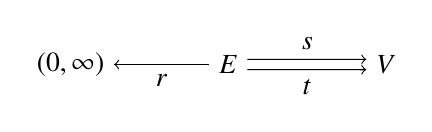
\begin{tikzpicture}[scale=2]
        \node (R) at (0,1) {$(0, \infty)$};
        \node (E1) at (1,1) {$E$}
          edge [->] node [below] {$r$} (R);
        \node (V1) at (2,1) {$V$};
        \draw [->] (E1.15) to node [above] {$s$} (V1.165);
        \draw [->] (E1.345) to node [below] {$t$} (V1.195);
      \end{tikzpicture}
    \end{center}
    There are various choices one could make for a morphism of such networks; Baez defined a morphism of resistor networks to be a pair of functions $\epsilon, \upsilon$ making the following diagrams commute:

    \begin{center}
      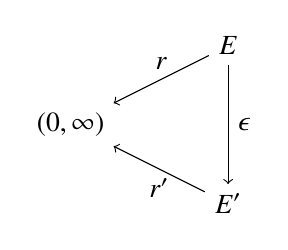
\begin{tikzpicture}[scale=2]
        \node (R) at (0,.5) {$(0, \infty)$};
        \node (E2) at (1, 0) {$E'$}
          edge [->] node [below] {$r'$} (R);
        \node (E1) at (1,1) {$E$}
          edge [->] node [above] {$r$} (R)
          edge [->] node [right] {$\epsilon$} (E2);
      \end{tikzpicture}
      $\quad$
      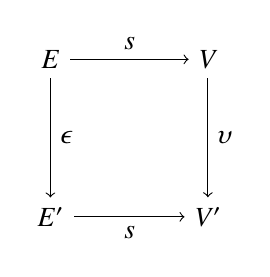
\begin{tikzpicture}[scale=2]
        \node (E2) at (1, 0) {$E'$};
        \node (E1) at (1,1) {$E$}
          edge [->] node [right] {$\epsilon$} (E2);
        \node (V2) at (2, 0) {$V'$}
          edge [<-] node [below] {$s$} (E2);
        \node (V1) at (2,1) {$V$}
          edge [<-] node [above] {$s$} (E1)
          edge [->] node [right] {$\upsilon$} (V2);
      \end{tikzpicture}
      $\quad$
      \begin{tikzpicture}[scale=2]
        \node (E2) at (1, 0) {$E'$};
        \node (E1) at (1,1) {$E$}
          edge [->] node [right] {$\epsilon$} (E2);
        \node (V2) at (2, 0) {$V'$}
          edge [<-] node [below] {$t$} (E2);
        \node (V1) at (2,1) {$V$}
          edge [<-] node [above] {$t$} (E1)
          edge [->] node [right] {$\upsilon$} (V2);
      \end{tikzpicture}
    \end{center}

    Resistor networks and morphisms between them form a category ResNet;
this category has finite limits and colimits.
    
    There is a compact closed bicategory Cospan(ResNet) with an important compact closed subbicategory Circ consisting of cospans whose feet are resistor networks with no edges.  A morphism in Circ is a {\bf circuit,} a resistor network with chosen sets of input and output vertices across which one can measure a voltage drop.
\end{itemize}

\section{Previous work}
\label{previous}

Compact closed categories were first defined by Kelly \cite{KellyCC}, and later studied in depth by Kelly and Laplaza \cite{KellyLaplaza}.

B\'enabou \cite{Ben67} defined bicategories and showed that small categories, distributors, and natural transformations form a bicategory Dist.  Distributors later became more widely known as ``profunctors'', so we will call that bicategory ``Prof'' instead.  Later, B\'enabou defined closed bicategories and showed that Prof is closed  \cite
{Ben73}.  He defined $V$-enriched profunctors when $V$ is a cocomplete monoidal or symmetric monoidal closed category, defined $V$-Prof and proved that any $V$-enriched functor, regarded as a $V$-profunctor, has a right adjoint.  More applications and details are in his lecture notes
\cite{Ben00}.

Kapranov and Voevodsky \cite{KV94} defined braided semistrict monoidal
2-categories, but their definition left out some necessary axioms.  Baez and Neuchl \cite{HDA1} gave an improved definition, but it was still missing a clause; Crans \cite{Crans} gave the complete definition.  See Baez and Langford \cite{HDA4} and Shulman \cite{Shulman} for details.

Gordon, Power, and Street \cite{GPS} defined fully weak tricategories; a monoidal bicategory is a one-object tricategory.

Another name for semistrict monoidal 2-categories is ``Gray monoids'', 
{\em i.e.} monoid objects in the 2-category Gray \cite{Gray}.  Day and Street \cite{DS97} defined compact closed Gray monoids, and appealed to the coherence theorem of Gordon, Power, and Street to extend compact closedness to arbitrary bicategories.  The semistrict approach is somewhat artificial when dealing with most ``naturally occurring''
bicategories, since the associator for composition of 1-morphisms is rarely the identity.  However, this approach does apply to Cocont.

Katis, Sabadini and Walters \cite{KSW98} gave a precise account of the double-entry bookkeeping method {\em partita doppia} in terms of the compact closed bicategory Span(RGraph); in a later paper \cite{KW99}, they cite a handwritten note by McCrudden for the ``swallowtail''
coherence law we use in this thesis.

Preller and Lambek \cite{PL07} generalized compact monoidal categories in a different direction.  They considered a compact monoidal category to be a one-object bicategory satisfying some criteria, and then extend that definition to multiple objects.  The resulting concept of ``compact bicategory'' is {\em not} what is being studied in this thesis.

McCrudden \cite{McCrudden} gave the first fully general definitions of braided, sylleptic, and symmetric monoidal bicategories.  Schommer-Pries
\cite{SPT} gave the correct notion of a monoidal transformation between monoidal functors between monoidal bicategories.

Carboni and Walters \cite{CW87} proved that $V$-Prof is a cartesian bicategory.  Later, they showed \cite{CW04} that Prof is equivalent to Cocont as a bicategory.  Together with Kelly and Wood \cite{CKWW08}, they proved that any cartesian bicategory is symmetric monoidal in the sense of McCrudden.

\section{Compact closed bicategories}
\label{definition}

In this section, we lay out the definition of a compact closed bicategory.  First we give the definition of a bicategory, then start adding structure to it: we introduce the tensor product and monoidal unit; then we look at the different ways to move objects around each other, giving braided, sylleptic and symmetric monoidal bicategories. Next, we define closed monoidal bicategories by introducing a right pseudoadjoint to tensoring with an object; and finally we introduce duals for objects in a bicategory.

\begin{defn}
  A {\bf bicategory} $\C$ consists of
  \begin{enumerate}
    \item a collection of {\bf objects}
    \item for each pair of objects $A, B$ in $\C$, a category $\C(A,B)$;
the objects of $\C(A,B)$ are called {\bf 1-morphisms}, while the morphisms of $\C(A,B)$ are called {\bf 2-morphisms}.
    \item for each triple of objects $A, B, C$ in $\C$, a {\bf composition} functor 
        \[ \circ_{A,B,C}\maps \C(B, C) \times \C(A, B) \to \C(A, C).\]
      We will leave off the indices and write it as an infix operator.
    \item for each object $A$ in $\C$, an object $1_A$ in $\C(A,A)$
called the {\bf identity 1-morphism on $A$}.  We will often write this simply as $A$.
    \item for each quadruple of objects $A, B, C, D$, a natural isomorphism called the {\bf associator for composition}; if $(f,g,h)$ is an object of $\C(C,D) \times \C(B,C) \times \C(A,B),$ then 
      $$\acirc_{f,g,h} \maps (f \circ g) \circ h \to f \circ (g
\circ h).$$
    \item for each pair of objects $A, B$ in $\C$, natural isomorphisms called {\bf left and right unitors for composition.}  If $f$ is an object of $\C(A,B)$, then
      \[\begin{array}{l}
        \lcirc_f\maps B \circ f \stackrel{\sim}{\to} f\\
        \rcirc_f\maps f \circ A \stackrel{\sim}{\to} f
      \end{array}\]
  \end{enumerate}
  such that $\acirc, \lcirc,$ and $\rcirc$ satisfy the following coherence laws:
  \begin{enumerate}
    \item for all $(f,g,h,j)$ in $\C(D,E) \times \C(C,D) \times \C(B,C)
\times \C(A,B),$ the following diagram, called the {\bf pentagon equation}, commutes:
      \[\begin{diagram}
        \node[2]{((f \circ g) \circ h) \circ j} \arrow{sse,t}{\acirc_{f\circ g, h, j}} \arrow{sw,t}{\acirc_{f,g,h} \circ j} \\
        \node{(f \circ (g \circ h)) \circ j} \arrow[2]{s,l}{\acirc_{f,g\circ h, j}}\\
        \node[3]{(f \circ g) \circ (h \circ j)} \arrow{ssw,b}{\acirc_{f,g,h \circ j}}\\
        \node{f \circ ((g \circ h) \circ j)} \arrow{se,b}{f \circ\acirc_{g,h,j}}\\
        \node[2]{f \circ (g \circ (h \circ j))}
      \end{diagram}\]
    \item for all $(f,g)$ in $\C(B,C)\times \C(A,B)$ the following diagram, called the {\bf triangle equation}, commutes:
      \[\begin{diagram}
        \node{(f \circ B) \circ g} 
          \arrow[2]{e,t}{\acirc} 
          \arrow{se,b} {\rcirc_f \circ g} \node[2]{f \circ (B \circ g)} 
          \arrow{sw,b}{f \circ \lcirc_g} \\
        \node[2]{f \circ g}
      \end{diagram}\]
  \end{enumerate}
\end{defn}

The associator $\acirc$ and unitors $\rcirc, \lcirc$ for composition of
1-morphisms are necessary, but when we are drawing commutative diagrams of 1-morphisms they are very hard to show; fortunately, by the coherence theorem for bicategories, any consistent choice is equivalent to any other, so we leave them out.

We refer the reader to Tom Leinster's excellent ``Basic bicategories''
\cite{LeinsterBB} for definitions of
\begin{itemize}
  \item morphisms of bicategories, which we call functors,
  \item transformations between functors, which we call pseudonatural transformations, and
  \item modifications between transformations.
\end{itemize}

\begin{defn}
  An {\bf equivalence} of objects $A, B$ in a bicategory is a pair of morphisms $f\maps A \to B, g\maps B \to A$ together with invertible 2-morphisms $e:g \circ f \stackrel{\sim}{\Rightarrow} 1_A$ and $i:f \circ g \stackrel{\sim}{\Rightarrow} 1_B$.
\end{defn}
\begin{defn}
  An {\bf adjoint equivalence} is one in which the 2-morphisms $e$ and $i^{-1}$ exhibit that $g$ is left adjoint to $f$.
\end{defn}
For a given morphism $f,$ any two choices of data $(g, e, i)$ making
$f$ an adjoint equivalence are canonically isomorphic, so any choice is as good as any other.  When $f, g$ form an adjoint equivalence, we write $g = f^\bullet$.  Any equivalence can be improved to an adjoint equivalence.

We can often take a 2-morphism and ``reverse'' one of its edges.  Given objects $A,B,C,D$, morphisms $f:A\to C$, $g:C\to D$, $h:D\to B$, $j:A
\to B$ such that $h$ is an adjoint equivalence, and a 2-morphism 
\begin{center}
  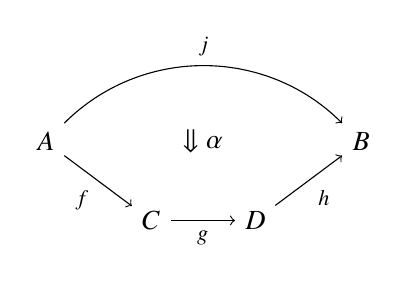
\begin{tikzpicture}[scale=2]
    \node (A) at (0,0) {$A$};
    \node (alpha) at (1,0) {$\Downarrow \alpha$};
    \node (C) at (.67, -.5) {$C$}
      edge [<-] node [below left, l] {$f$} (A);
    \node (D) at (1.33, -.5) {$D$}
      edge [<-] node [below, l] {$g$} (C);
    \node (B) at (2,0) {$B$}
      edge [<-, out=135, in=45] node [above,l] {$j$} (A)
      edge [<-] node [below right, l] {$h$} (D);
  \end{tikzpicture}
\end{center}
we can get a new 2-morphism 
\[ (\rcirc(g) \circ f)(e_h \circ g \circ f)(h^\bullet \circ
\alpha):h^\bullet \circ j \Rightarrow g \circ f, \]
\begin{center}
  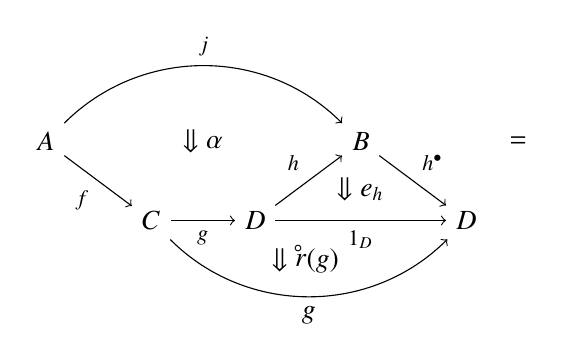
\begin{tikzpicture}[scale=2]
    \node (A) at (0,0) {$A$};
    \node (alpha) at (1,0) {$\Downarrow \alpha$};
    \node (C) at (.67, -.5) {$C$}
      edge [<-] node [below left, l] {$f$} (A);
    \node (D) at (1.33, -.5) {$D$}
      edge [<-] node [below, l] {$g$} (C);
    \node (B) at (2,0) {$B$}
      edge [<-, out=135, in=45] node [above,l] {$j$} (A)
      edge [<-] node [above left, l] {$h$} (D);
    \node (D2) at (2.67, -.5) {$D$}
      edge [<-] node [above right, l] {$h^\bullet$} (B)
      edge [<-] node [below, l] {$1_D$} (D)
      edge [<-, out=-135, in=-45] node [below] {$g$} (C);
    \node at (2, -.3) {$\Downarrow e_h$};
    \node at (1.65, -.75) {$\Downarrow \rcirc(g)$};
    \node at (3,0) {$=$};
  \end{tikzpicture}  
  \begin{tikzpicture}[scale=2]
    \node (A) at (0,0) {$A$};
    \node (alpha) at (1,0) {$\Downarrow \alpha_1$};
    \node (C) at (.67, -.5) {$C$}
      edge [<-] node [below left, l] {$f$} (A);
    \node (D) at (1.33, -.5) {$D$}
      edge [<-] node [below, l] {$g$} (C);
    \node (B) at (2,0) {$B$}
      edge [<-, out=135, in=45] node [above,l] {$j$} (A)
      edge [->] node [below right, l] {$h^\bullet$} (D);
    \node at (0,-1.2) {};
  \end{tikzpicture}  
\end{center}
where $e_h:h^\bullet \circ h \Rightarrow 1$ is the 2-morphism from the equivalence.  We denote such variations of a 2-morphism by adding numeric subscripts; the number simply records the order in which we introduce them, not any information about the particular variation.

In the following definitions, I have given some plausible combinatorical reasoning justifying many of the parts of the definition, but except where noted, this is not part of the definition; its intent is merely to help organize the rather long and dry content.  I am not aware of any work on the combinatorics of cells in higher categories beyond that mentioned below by Stasheff, Kapranov and Voevodsky.  

Also, in the illustrations of 2-cells and coherence laws below, I use expressions like $(A \tensor B) \tensor C$ as a shorthand for functors like
      \[\tensor \circ (\tensor \times 1): \C^3 \to \C.\]

\begin{defn} A {\bf monoidal bicategory} $\C$ is a bicategory in which we can ``multiply'' objects.  It consists of the following: \\
  
\begin{itemize}
\item A bicategory $\C$.
\item A {\bf tensor product} functor $\otimes:\C \times \C \rightarrow
\C$.  This functor involves an invertible ``tensorator'' 2-morphism
$(f \otimes g) \circ (f' \otimes g') \Rightarrow 
(f \circ f') \otimes (g \circ g')$ which we elide in most of the coherence equations below.  The coherence theorem for monoidal bicategories implies that any 2-morphism involving the tensorator is the same no matter how it is inserted \cite[Remark~3.1.6]{Gurski}, so like the associator for composition of 1-morphisms, we leave it out.

The {\bf Stasheff polytopes} \cite{Stasheff} are a series of geometric figures whose vertices enumerate the ways to parenthesize the tensor product of $n$ objects, so the number of vertices is given by the Catalan numbers; for each polytope, we have a corresponding $(n-2)$-morphism of the same shape with directed edges and faces:
  \begin{enumerate}
    \item The tensor product of one object $A$ is the one object $A$ itself.
    \item The tensor product of two objects $A$ and $B$ is the one object $A \tensor B$.
    \item There are two ways to parenthesize the product of three objects, so we have an {\bf associator} adjoint equivalence pseudonatural in $A,B,C$
        \[ a\maps (A\tensor B) \tensor C \rightarrow A \tensor (B\tensor C) \]
      for moving parentheses from the left pair to the right pair.
    \item There are five ways to parenthesize the product of four objects, so we have a {\bf pentagonator} invertible modification $\pi$ relating the two different ways of moving parentheses from being clustered at the left to being clustered at the right.  (Mnemonic: Pink Pentagonator.)
      \begin{center}
        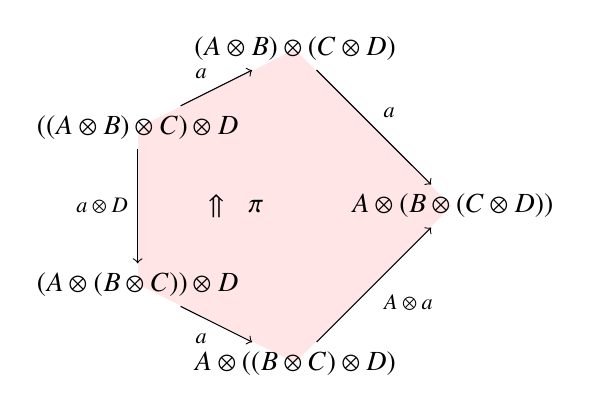
\begin{tikzpicture}
          \filldraw[white,fill=red,fill opacity=0.1](0,3)--(2,4)--(4,2)--(2,0)--(0,1)--cycle;
          \node (ABCD1) at (0,3) {$((A \tensor B) \tensor C) \tensor D$};
          \node (ABCD2) at (2,4) {$(A\tensor B) \tensor (C\tensor D)$}
            edge [<-] node [l, above left] {$a$} (ABCD1);
          \node (ABCD3) at (4,2) {$A \tensor (B \tensor (C \tensor D))$}
            edge [<-] node [l, above right] {$a$} (ABCD2);
          \node (ABCD4) at (2,0) {$A \tensor ((B \tensor C) \tensor D)$}
            edge [->] node [l, below right] {$A \tensor a$} (ABCD3);
          \node (ABCD5) at (0,1) {$(A \tensor (B \tensor C)) \tensor D$}
            edge [->] node [l, below left] {$a$} (ABCD4)
            edge [<-] node [l, left] {$a \tensor D$} (ABCD1);
          \node at (1,2) {\tikz\node [rotate=90] {$\Rightarrow$};};
          \node at (1.5,2) {$\pi$};
        \end{tikzpicture}
      \end{center}
    \item There are fourteen ways to parenthesize the product of five objects, so we have an {\bf associahedron} equation of modifications with fourteen vertices relating the various ways of getting from the parentheses clustered at the left to clustered at the right.
      \begin{center}
        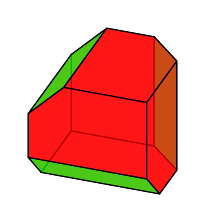
\begin{tikzpicture}[line join=round]
          \begin{scope}[scale=.2]
            \filldraw[fill=red,fill opacity=0.7](-4.306,-3.532)--(-2.391,-.901)--(-2.391,3.949)--(-5.127,.19)--(-5.127,-2.581)--cycle;
            \filldraw[fill=red,fill opacity=0.7](-4.306,-3.532)--(-2.391,-.901)--(2.872,-1.858)--(4.306,-3.396)--(3.212,-4.9)--cycle;
            \filldraw[fill=red,fill opacity=0.7](2.872,-1.858)--(2.872,5.07)--(-.135,5.617)--(-2.391,3.949)--(-2.391,-.901)--cycle;
            \filldraw[fill=green,fill opacity=0.7](4.306,-3.396)--(4.306,3.532)--(2.872,5.07)--(2.872,-1.858)--cycle;
            \filldraw[fill=green,fill opacity=0.7](-2.872,1.858)--(-.135,5.617)--(-2.391,3.949)--(-5.127,.19)--cycle;
            \filldraw[fill=red,fill opacity=0.7](3.212,-4.9)--(4.306,-3.396)--(4.306,3.532)--(2.391,.901)--(2.391,-3.949)--cycle;
            \filldraw[fill=green,fill opacity=0.7](-4.306,-3.532)--(3.212,-4.9)--(2.391,-3.949)--(-5.127,-2.581)--cycle;
            \filldraw[fill=red,fill opacity=0.7](-2.872,1.858)--(2.391,.901)--(4.306,3.532)--(2.872,5.07)--(-.135,5.617)--cycle;
            \filldraw[fill=red,fill opacity=0.7](-5.127,-2.581)--(-5.127,.19)--(-2.872,1.858)--(2.391,.901)--(2.391,-3.949)--cycle;
          \end{scope}
        \end{tikzpicture}% End sketch output
      \end{center}
    The associahedron is a cube with three of its edges bevelled. It holds in the bicategory $\C$, where we have used juxtaposition instead of $\tensor$ for brevity and the unmarked 2-morphisms are instances of the pseudonaturality invertible modification for the associator.  (Mnemonic for the rectangular invertible modifications: GReen conGRuences.)
      \begin{center}
        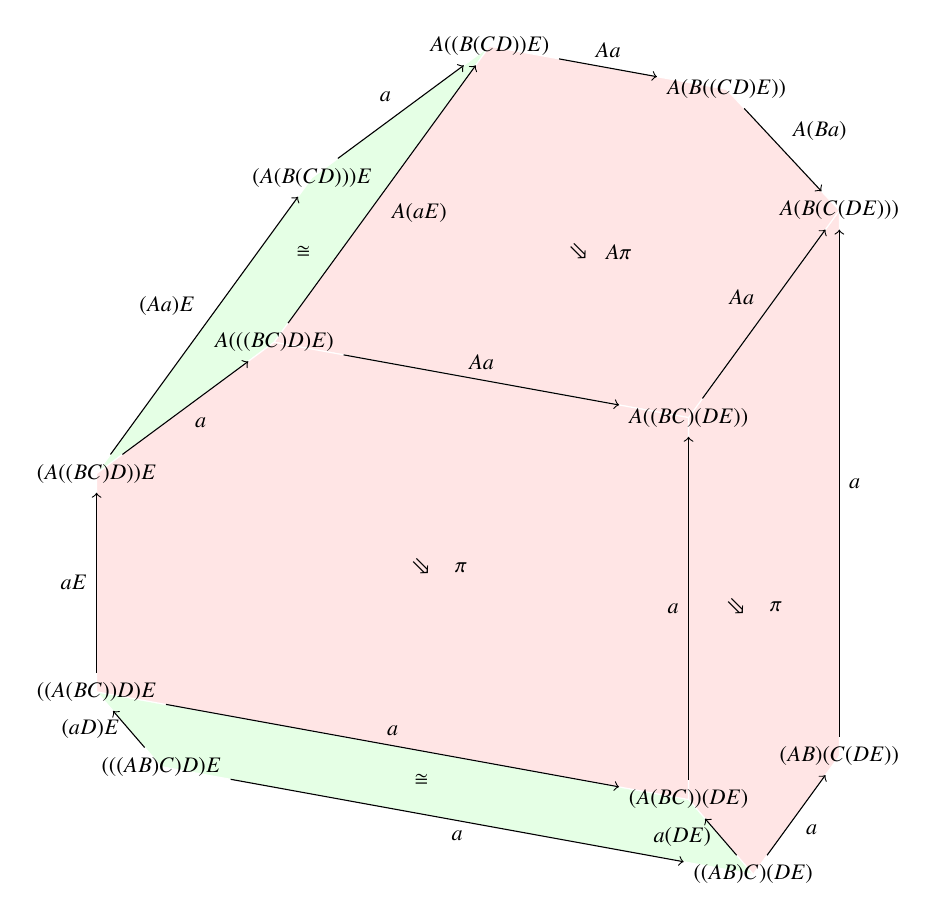
\begin{tikzpicture}[line join=round]
          \filldraw[white,fill=green,fill opacity=0.1](-2.872,1.858)--(-.135,5.617)--(-2.391,3.949)--(-5.127,.19)--cycle;
          \filldraw[white,fill=red,fill opacity=0.1](3.212,-4.9)--(4.306,-3.396)--(4.306,3.532)--(2.391,.901)--(2.391,-3.949)--cycle;
          \filldraw[white,fill=green,fill opacity=0.1](-4.306,-3.532)--(3.212,-4.9)--(2.391,-3.949)--(-5.127,-2.581)--cycle;
          \filldraw[white,fill=red,fill opacity=0.1](-2.872,1.858)--(2.391,.901)--(4.306,3.532)--(2.872,5.07)--(-.135,5.617)--cycle;
          \filldraw[white,fill=red,fill opacity=0.1](-5.127,-2.581)--(-5.127,.19)--(-2.872,1.858)--(2.391,.901)--(2.391,-3.949)--cycle;
          \begin{scope}[font=\fontsize{8}{8}\selectfont]
            \node (A) at (-2.391,3.949) {$(A(B(CD)))E$};
            \node (B) at (-5.127,.19) {$(A((BC)D))E$}
              edge [->] node [l, above left] {$(Aa)E$} (A);
            \node (C) at (-5.127,-2.581) {$((A(BC))D)E$}
              edge [->] node [l, left] {$aE$} (B);
            \node (D) at (-4.306,-3.532) {$(((AB)C)D)E$}
              edge [->] node [l, left] {$(aD)E$} (C);
            \node (E) at (3.212,-4.9) {$((AB)C)(DE)$}
              edge [<-] node [l, below] {$a$} (D);
            \node (F) at (4.306,-3.396) {$(AB)(C(DE))$}
              edge [<-] node [l, below right] {$a$} (E);
            \node (G) at (4.306,3.532) {$A(B(C(DE)))$}
              edge [<-] node [l, right] {$a$} (F);
            \node (H) at (2.872,5.07) {$A(B((CD)E))$}
              edge [->] node [l, above right] {$A(Ba)$} (G);
            \node (I) at (-.135,5.617) {$A((B(CD))E)$}
              edge [->] node [l, above] {$Aa$} (H)
              edge [<-] node [l, above left] {$a$} (A);
            \node (J) at (-2.872,1.858) {$A(((BC)D)E)$}
              edge [->] node [l, below right] {$A(aE)$} (I)
              edge [<-] node [l, below right] {$a$} (B);
            \node (K) at (2.391,-3.949) {$(A(BC))(DE)$}
              edge [<-] node [l, left] {$a(DE)$} (E)
              edge [<-] node [l, above] {$a$} (C);
            \node (L) at (2.391,.901) {$A((BC)(DE))$}
              edge [<-] node [l, left] {$a$} (K)
              edge [<-] node [l, above] {$Aa$} (J)
              edge [->] node [l, above left] {$Aa$} (G);
            \node at (-1,-1) {\tikz\node [rotate=-45] {$\Rightarrow$};};
            \node at (-.5,-1) {$\pi$};
            \node at (1,3) {\tikz\node [rotate=-45] {$\Rightarrow$};};
            \node at (1.5,3) {$A \pi$};
            \node at (3,-1.5) {\tikz\node [rotate=-45] {$\Rightarrow$};};
            \node at (3.5,-1.5) {$\pi$};
            \node at (-1,-3.7) {$\cong$};
            \node at (-2.5,3) {$\cong$};
          \end{scope}
        \end{tikzpicture}% End sketch output
        \\
        =
        \\
        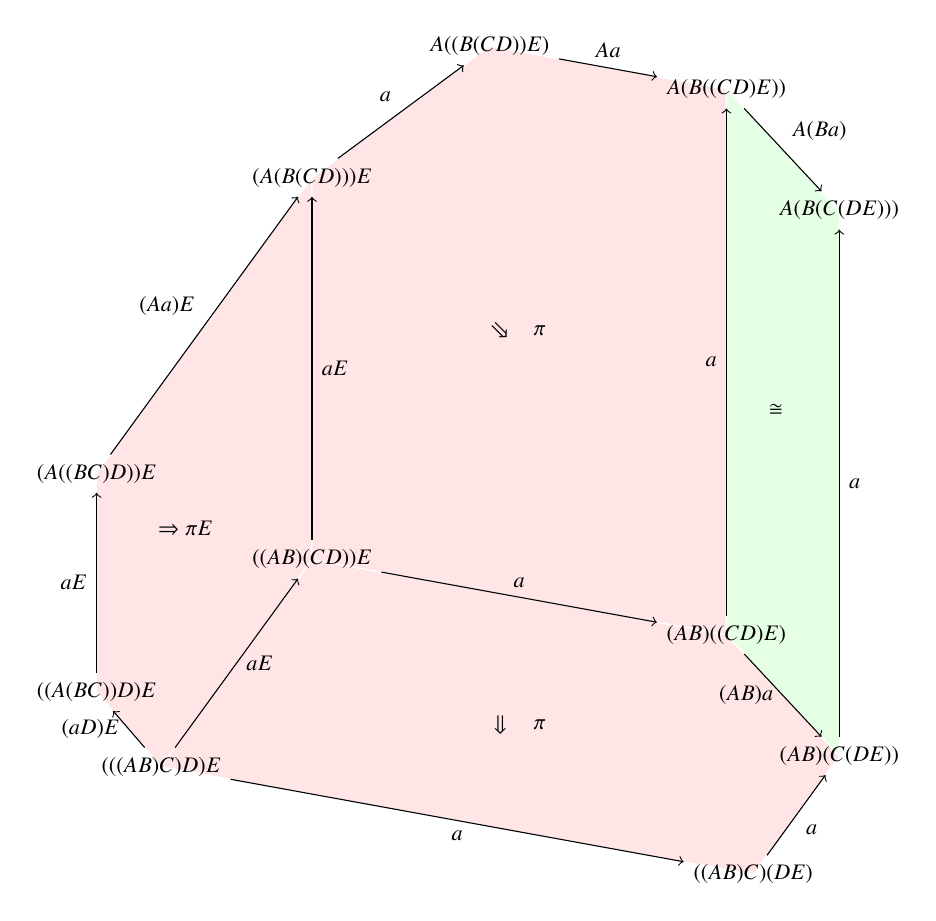
\begin{tikzpicture}[line join=round]
          \filldraw[white,fill=red,fill opacity=0.1](-4.306,-3.532)--(-2.391,-.901)--(-2.391,3.949)--(-5.127,.19)--(-5.127,-2.581)--cycle;
          \filldraw[white,fill=red,fill opacity=0.1](-4.306,-3.532)--(-2.391,-.901)--(2.872,-1.858)--(4.306,-3.396)--(3.212,-4.9)--cycle;
          \filldraw[white,fill=red,fill opacity=0.1](2.872,-1.858)--(2.872,5.07)--(-.135,5.617)--(-2.391,3.949)--(-2.391,-.901)--cycle;
          \filldraw[white,fill=green,fill opacity=0.1](4.306,-3.396)--(4.306,3.532)--(2.872,5.07)--(2.872,-1.858)--cycle;
          \begin{scope}[font=\fontsize{8}{8}\selectfont]
            \node (A) at (-2.391,3.949) {$(A(B(CD)))E$};
            \node (B) at (-5.127,.19) {$(A((BC)D))E$}
              edge [->] node [l, above left] {$(Aa)E$} (A);
            \node (C) at (-5.127,-2.581) {$((A(BC))D)E$}
              edge [->] node [l, left] {$aE$} (B);
            \node (D) at (-4.306,-3.532) {$(((AB)C)D)E$}
              edge [->] node [l, left] {$(aD)E$} (C);
            \node (E) at (3.212,-4.9) {$((AB)C)(DE)$}
              edge [<-] node [l, below] {$a$} (D);
            \node (F) at (4.306,-3.396) {$(AB)(C(DE))$}
              edge [<-] node [l, below right] {$a$} (E);
            \node (G) at (4.306,3.532) {$A(B(C(DE)))$}
              edge [<-] node [l, right] {$a$} (F);
            \node (H) at (2.872,5.07) {$A(B((CD)E))$}
              edge [->] node [l, above right] {$A(Ba)$} (G);
            \node (I) at (-.135,5.617) {$A((B(CD))E)$}
              edge [->] node [l, above] {$Aa$} (H)
              edge [<-] node [l, above left] {$a$} (A);
            \node (M) at (-2.391,-.901) {$((AB)(CD))E$}
              edge [<-] node [l, right] {$aE$} (D)
              edge [->] node [l, right] {$aE$} (A);
            \node (N) at (2.872,-1.858) {$(AB)((CD)E)$}
              edge [<-] node [l, above] {$a$} (M)
              edge [->] node [l, left] {$a$} (H)
              edge [->] node [l, left] {$(AB)a$} (F);
            \node at (-4,-.5) {$\Rightarrow \pi E$};
            \node at (0,-3) {\tikz\node [rotate=-90] {$\Rightarrow$};};
            \node at (0.5,-3) {$\pi$};
            \node at (0,2) {\tikz\node [rotate=-45] {$\Rightarrow$};};
            \node at (0.5,2) {$\pi$};
            \node at (3.5,1) {$\cong$};
          \end{scope}
        \end{tikzpicture}% End sketch output
      \end{center}
  
  \end{enumerate}

\item Just as in any monoid there is an identity element 1, in every monoidal bicategory there is a {\bf monoidal unit} object $I$. Associated to the monoidal unit are a series of morphisms---one of each dimension---that express how to ``cancel'' the unit in a product. Each morphism of dimension $n>0$ has two Stasheff polytopes of dimension $n-1$ as ``subcells'', one for parenthesizing $n+1$ objects and the other for parenthesizing the $n$ objects left over after cancellation.  There are $n+1$ ways to insert $I$ into $n$ objects, so there are $n+1$ morphisms of dimension $n$.
  \begin{enumerate}
    \item There is one monoidal unit object $I$.
    \item There are two {\bf unitor} adjoint equivalences $l$ and $r$ that are pseudonatural in $A$.  The Stasheff polytopes for two objects and for one object are both points, so the unitors are line segments joining them.
        \[ l\maps I \tensor A \rightarrow A \]
        \[ r\maps A \tensor I \rightarrow A. \]
    \item There are three {\bf 2-unitor} invertible modifications $\lambda, \mu,$ and $\rho$. The Stasheff polytope for three objects is a line segment and the Stasheff polytope for two objects is a point, so these modifications are triangles.  (Mnemonic: Umber Unitor.)
      \begin{center}
        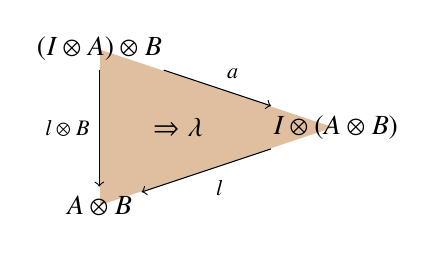
\begin{tikzpicture}
          \filldraw[white,fill=brown,fill opacity=0.5](0,2)--(3,1)--(0,0)--cycle;
          \node (IAB1) at (0,2) {$(I\tensor A)\tensor B$};
          \node (IAB2) at (3,1) {$I\tensor (A \tensor B)$}
            edge [<-] node [l, above right] {$a$} (IAB1);
          \node (AB) at (0,0) {$A \tensor B$}
            edge [<-] node [l, below right] {$l$} (IAB2)
            edge [<-] node [l, left] {$l \tensor B$} (IAB1);
          \node at (1,1) {$\Rightarrow \lambda$};
        \end{tikzpicture}
      \end{center}
      \begin{center}
        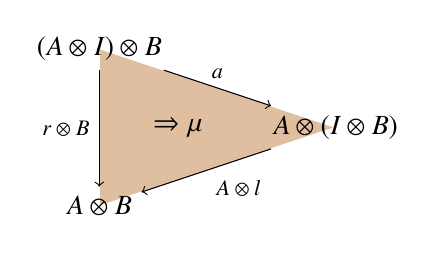
\begin{tikzpicture}
          \filldraw[white,fill=brown,fill opacity=0.5](0,2)--(3,1)--(0,0)--cycle;
          \node (AB) at (0,0) {$A \tensor B$};
          \node (AIB2) at (3,1) {$A\tensor (I\tensor B)$}
            edge [->] node [l, below right] {$A \tensor l$} (AB);
          \node (AIB1) at (0,2) {$(A\tensor I) \tensor B$}
            edge [->] node [l, above] {$a$} (AIB2)
            edge [->] node [l, left] {$r \tensor B$} (AB);
          \node at (1,1) {$\Rightarrow \mu$};
        \end{tikzpicture}
      \end{center}
      \begin{center}
        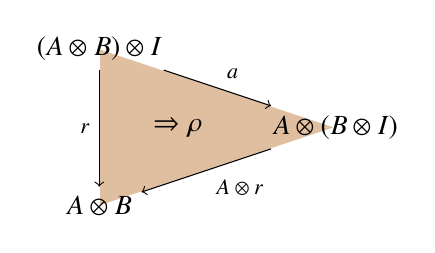
\begin{tikzpicture}
          \filldraw[white,fill=brown,fill opacity=0.5](0,2)--(3,1)--(0,0)--cycle;
          \node (ABI1) at (0,2) {$(A \tensor B) \tensor I$};
          \node (ABI2) at (3,1) {$A \tensor (B \tensor I)$}
            edge [<-] node [l, above right] {$a$} (ABI1);
          \node (AB) at (0,0) {$A \tensor B$}
            edge [<-] node [l, below right] {$A \tensor r$} (ABI2)
            edge [<-] node [l, left] {$r$} (ABI1);
          \node at (1,1) {$\Rightarrow \rho$};
        \end{tikzpicture}
      \end{center}
    \item There are four equations of modifications.  The Stasheff polytope for four objects is a pentagon and the Stasheff polytope for three objects is a line segment, so these equations are irregular prisms with seven vertices.

% IBCD
    \begin{center}
      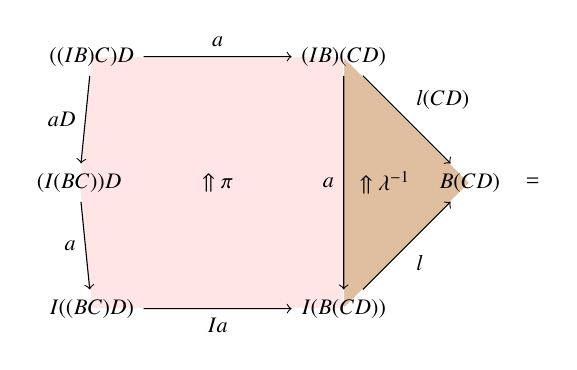
\begin{tikzpicture}[scale=1.6]
        \filldraw[white,fill=red,fill opacity=0.1](-1,1)--(1,1)--(1,-1)--(-1,-1)--(-1.1,0)--cycle;
        \filldraw[white,fill=brown,fill opacity=0.5](1,1)--(2,0)--(1,-1)--cycle;
        \begin{scope}[font=\fontsize{8}{8}\selectfont]
          \node (A) at (-1.1,0) {$(I(BC))D$};
          \node (B) at (-1,1) {$((IB)C)D$}
            edge [->] node [l, left] {$aD$} (A);
          \node (C) at (1,1) {$(IB)(CD)$}
            edge [<-] node [l, above] {$a$} (B);
          \node (D) at (1,-1) {$I(B(CD))$}
            edge [<-] node [l, left] {$a$} (C);
          \node (E) at (-1,-1) {$I((BC)D)$}
            edge [->] node [l, below] {$Ia$} (D)
            edge [<-] node [l, left] {$a$} (A);
          \node (F) at (2,0) {$B(CD)$}
            edge [<-] node [l, above right] {$l(CD)$} (C)
            edge [<-] node [l, below right] {$l$} (D);
          \node at (0,0) {$\Uparrow \pi$};
          \node at (1.33,0) {$\Uparrow \lambda^{-1}$};
          \node at (2.5, 0) {=};
        \end{scope}
      \end{tikzpicture}
      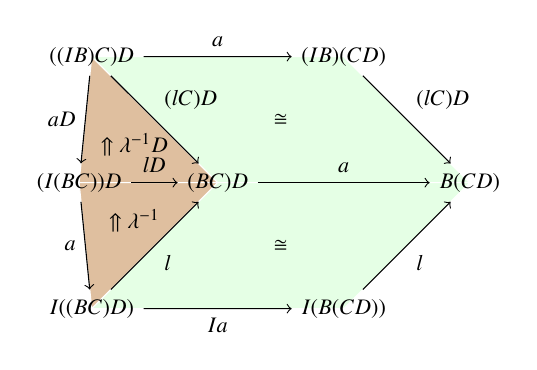
\begin{tikzpicture}[scale=1.6]
        \filldraw[white,fill=brown,fill opacity=0.5](-1,1)--(0,0)--(-1.1,0)--cycle;
        \filldraw[white,fill=brown,fill opacity=0.5](-1,-1)--(0,0)--(-1.1,0)--cycle;
        \filldraw[white,fill=green,fill opacity=0.1](-1,1)--(0,0)--(2,0)--(1,1)--cycle;
        \filldraw[white,fill=green,fill opacity=0.1](-1,-1)--(0,0)--(2,0)--(1,-1)--cycle;
        \begin{scope}[font=\fontsize{8}{8}\selectfont]
          \node (A) at (-1.1,0) {$(I(BC))D$};
          \node (B) at (-1,1) {$((IB)C)D$}
            edge [->] node [l, left] {$aD$} (A);
          \node (C) at (1,1) {$(IB)(CD)$}
            edge [<-] node [l, above] {$a$} (B);
          \node (D) at (1,-1) {$I(B(CD))$};
          \node (E) at (-1,-1) {$I((BC)D)$}
            edge [->] node [l, below] {$Ia$} (D)
            edge [<-] node [l, left] {$a$} (A);
          \node (F) at (2,0) {$B(CD)$}
            edge [<-] node [l, above right] {$(lC)D$} (C)
            edge [<-] node [l, below right] {$l$} (D);
          \node (G) at (0,0) {$(BC)D$}
            edge [<-] node [l, above] {$lD$} (A)
            edge [<-] node [l, above right] {$(lC)D$} (B)
            edge [<-] node [l, below right] {$l$} (E)
            edge [->] node [l, above] {$a$} (F);
          \node at (-.66,.3) {$\Uparrow \lambda^{-1} D$};
          \node at (-.66,-.3) {$\Uparrow \lambda^{-1}$};
          \node at (.5,.5) {$\cong$};
          \node at (.5,-.5) {$\cong$};
        \end{scope}
      \end{tikzpicture}
    \end{center}
% AICD
    \begin{center}
      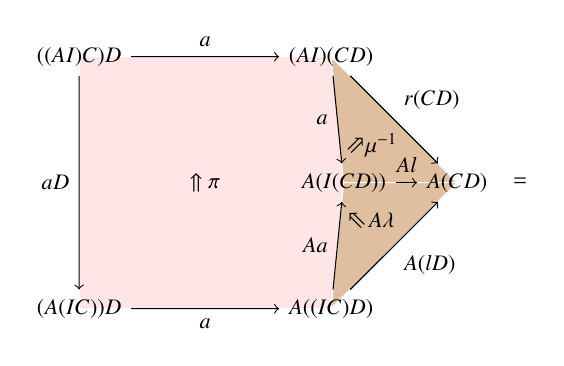
\begin{tikzpicture}[scale=1.6]
        \filldraw[white,fill=red,fill opacity=0.1](-1,-1)--(-1,1)--(1,1)--(1.1,0)--(1,-1)--cycle;
        \filldraw[white,fill=brown,fill opacity=0.5](1,1)--(1.1,0)--(2,0)--cycle;
        \filldraw[white,fill=brown,fill opacity=0.5](1.1,0)--(1,-1)--(2,0)--cycle;
        \begin{scope}[font=\fontsize{8}{8}\selectfont]
          \node (A) at (-1,1) {$((AI)C)D$};
          \node (B) at (1,1) {$(AI)(CD)$}
            edge [<-] node [l,above] {$a$} (A);
          \node (C) at (1.1,0) {$A(I(CD))$}
            edge [<-] node [l,left] {$a$} (B);
          \node (D) at (1,-1) {$A((IC)D)$}
            edge [->] node [l,left] {$Aa$} (C);
          \node (E) at (-1,-1) {$(A(IC))D$}
            edge [->] node [l,below] {$a$} (D)
            edge [<-] node [l,left] {$aD$} (A);
          \node (F) at (2,0) {$A(CD)$}
            edge [<-] node [l,above right] {$r(CD)$} (B)
            edge [<-] node [l,above] {$Al$} (C)
            edge [<-] node [l,below right] {$A(lD)$} (D);
          \node at (0,0) {$\Uparrow \pi$};
          \node at (1.2,.3) {\tikz\node [rotate=45] {$\Rightarrow$};};
          \node at (1.4,.3) {$\mu^{-1}$};
          \node at (1.2,-.3) {\tikz\node [rotate=135] {$\Rightarrow$};};
          \node at (1.4,-.3) {$A\lambda$};
          \node at (2.5,0) {=};
        \end{scope}
      \end{tikzpicture}
      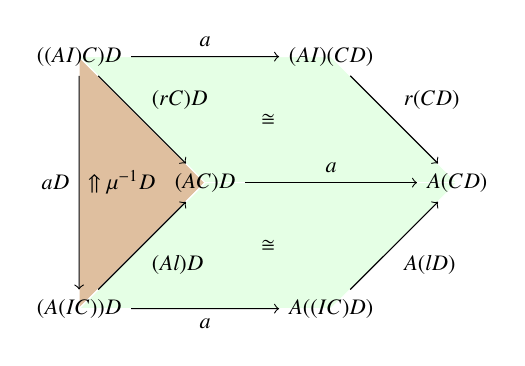
\begin{tikzpicture}[scale=1.6]
        \filldraw[white,fill=brown,fill opacity=0.5](-1,1)--(0,0)--(-1,-1)--cycle;
        \filldraw[white,fill=green,fill opacity=0.1](-1,1)--(0,0)--(2,0)--(1,1)--cycle;
        \filldraw[white,fill=green,fill opacity=0.1](0,0)--(2,0)--(1,-1)--(-1,-1)--cycle;
        \begin{scope}[font=\fontsize{8}{8}\selectfont]
          \node (A) at (-1,1) {$((AI)C)D$};
          \node (B) at (1,1) {$(AI)(CD)$}
            edge [<-] node [l,above] {$a$} (A);
          \node (D) at (1,-1) {$A((IC)D)$};
          \node (E) at (-1,-1) {$(A(IC))D$}
            edge [->] node [l,below] {$a$} (D)
            edge [<-] node [l,left] {$aD$} (A);
          \node (F) at (2,0) {$A(CD)$}
            edge [<-] node [l,above right] {$r(CD)$} (B)
            edge [<-] node [l,below right] {$A(lD)$} (D);
          \node (G) at (0,0) {$(AC)D$}
            edge [<-] node [l,above right] {$(rC)D$} (A)
            edge [<-] node [l,below right] {$(Al)D$} (E)
            edge [->] node [l, above] {$a$} (F);
          \node at (-.66,0) {$\Uparrow \mu^{-1}D$};
          \node at (.5,.5) {$\cong$};
          \node at (.5,-.5) {$\cong$};
        \end{scope}
      \end{tikzpicture}
    \end{center}
% ABID
    \begin{center}
      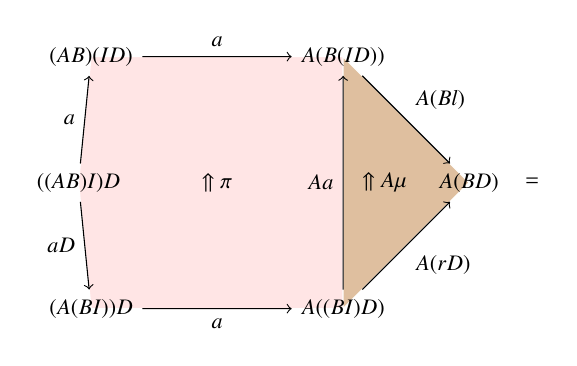
\begin{tikzpicture}[scale=1.6]
        \filldraw[white,fill=red,fill opacity=0.1](-1,1)--(1,1)--(1,-1)--(-1,-1)--(-1.1,0)--cycle;
        \filldraw[white,fill=brown,fill opacity=0.5](1,1)--(2,0)--(1,-1)--cycle;
        \begin{scope}[font=\fontsize{8}{8}\selectfont]
          \node (A) at (-1.1,0) {$((AB)I)D$};
          \node (B) at (-1,1) {$(AB)(ID)$}
            edge [<-] node [l, left] {$a$} (A);
          \node (C) at (1,1) {$A(B(ID))$}
            edge [<-] node [l, above] {$a$} (B);
          \node (D) at (1,-1) {$A((BI)D)$}
            edge [->] node [l, left] {$Aa$} (C);
          \node (E) at (-1,-1) {$(A(BI))D$}
            edge [->] node [l, below] {$a$} (D)
            edge [<-] node [l, left] {$aD$} (A);
          \node (F) at (2,0) {$A(BD)$}
            edge [<-] node [l, above right] {$A(Bl)$} (C)
            edge [<-] node [l, below right] {$A(rD)$} (D);
          \node at (0,0) {$\Uparrow \pi$};
          \node at (1.33,0) {$\Uparrow A\mu$};
          \node at (2.5, 0) {=};
        \end{scope}
      \end{tikzpicture}
      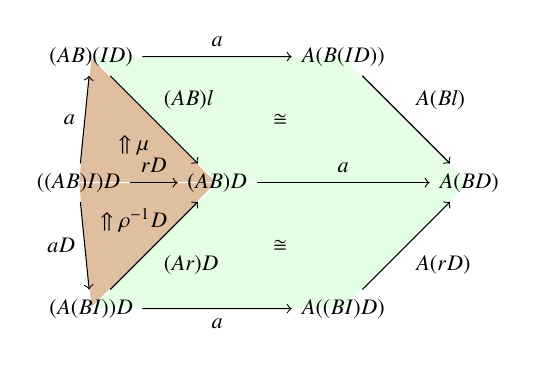
\begin{tikzpicture}[scale=1.6]
        \filldraw[white,fill=brown,fill opacity=0.5](-1,1)--(0,0)--(-1.1,0)--cycle;
        \filldraw[white,fill=brown,fill opacity=0.5](-1,-1)--(0,0)--(-1.1,0)--cycle;
        \filldraw[white,fill=green,fill opacity=0.1](-1,1)--(0,0)--(2,0)--(1,1)--cycle;
        \filldraw[white,fill=green,fill opacity=0.1](-1,-1)--(0,0)--(2,0)--(1,-1)--cycle;
        \begin{scope}[font=\fontsize{8}{8}\selectfont]
          \node (A) at (-1.1,0) {$((AB)I)D$};
          \node (B) at (-1,1) {$(AB)(ID)$}
            edge [<-] node [l, left] {$a$} (A);
          \node (C) at (1,1) {$A(B(ID))$}
            edge [<-] node [l, above] {$a$} (B);
          \node (D) at (1,-1) {$A((BI)D)$};
          \node (E) at (-1,-1) {$(A(BI))D$}
            edge [->] node [l, below] {$a$} (D)
            edge [<-] node [l, left] {$aD$} (A);
          \node (F) at (2,0) {$A(BD)$}
            edge [<-] node [l, above right] {$A(Bl)$} (C)
            edge [<-] node [l, below right] {$A(rD)$} (D);
          \node (G) at (0,0) {$(AB)D$}
            edge [<-] node [l, above] {$rD$} (A)
            edge [<-] node [l, above right] {$(AB)l$} (B)
            edge [<-] node [l, below right] {$(Ar)D$} (E)
            edge [->] node [l, above] {$a$} (F);
          \node at (-.66,.3) {$\Uparrow \mu$};
          \node at (-.66,-.3) {$\Uparrow \rho^{-1}D$};
          \node at (.5,.5) {$\cong$};
          \node at (.5,-.5) {$\cong$};
        \end{scope}
      \end{tikzpicture}
    \end{center}
% ABCI
    \begin{center}
      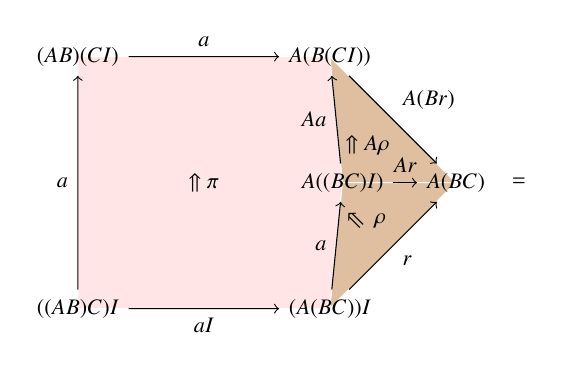
\begin{tikzpicture}[scale=1.6]
        \filldraw[white,fill=red,fill opacity=0.1](-1,-1)--(-1,1)--(1,1)--(1.1,0)--(1,-1)--cycle;
        \filldraw[white,fill=brown,fill opacity=0.5](1,1)--(1.1,0)--(2,0)--cycle;
        \filldraw[white,fill=brown,fill opacity=0.5](1.1,0)--(1,-1)--(2,0)--cycle;
        \begin{scope}[font=\fontsize{8}{8}\selectfont]
          \node (A) at (-1,1) {$(AB)(CI)$};
          \node (B) at (1,1) {$A(B(CI))$}
            edge [<-] node [l,above] {$a$} (A);
          \node (C) at (1.1,0) {$A((BC)I)$}
            edge [->] node [l,left] {$Aa$} (B);
          \node (D) at (1,-1) {$(A(BC))I$}
            edge [->] node [l,left] {$a$} (C);
          \node (E) at (-1,-1) {$((AB)C)I$}
            edge [->] node [l,below] {$aI$} (D)
            edge [->] node [l,left] {$a$} (A);
          \node (F) at (2,0) {$A(BC)$}
            edge [<-] node [l,above right] {$A(Br)$} (B)
            edge [<-] node [l,above] {$Ar$} (C)
            edge [<-] node [l,below right] {$r$} (D);
          \node at (0,0) {$\Uparrow \pi$};
          \node at (1.3,.3) {$\Uparrow A\rho$};
          \node at (1.2,-.3) {\tikz\node [rotate=135] {$\Rightarrow$};};
          \node at (1.4,-.3) {$\rho$};
          \node at (2.5,0) {=};
        \end{scope}
      \end{tikzpicture}
      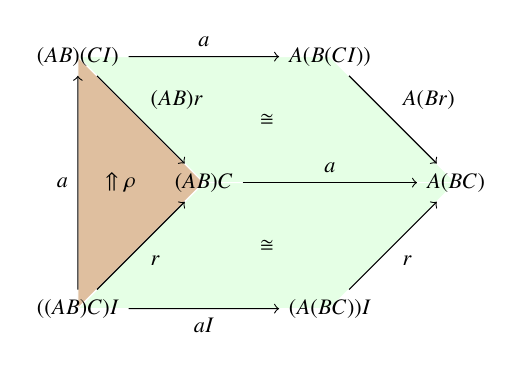
\begin{tikzpicture}[scale=1.6]
        \filldraw[white,fill=brown,fill opacity=0.5](-1,1)--(0,0)--(-1,-1)--cycle;
        \filldraw[white,fill=green,fill opacity=0.1](-1,1)--(0,0)--(2,0)--(1,1)--cycle;
        \filldraw[white,fill=green,fill opacity=0.1](0,0)--(2,0)--(1,-1)--(-1,-1)--cycle;
        \begin{scope}[font=\fontsize{8}{8}\selectfont]
          \node (A) at (-1,1) {$(AB)(CI)$};
          \node (B) at (1,1) {$A(B(CI))$}
            edge [<-] node [l,above] {$a$} (A);
          \node (D) at (1,-1) {$(A(BC))I$};
          \node (E) at (-1,-1) {$((AB)C)I$}
            edge [->] node [l,below] {$aI$} (D)
            edge [->] node [l,left] {$a$} (A);
          \node (F) at (2,0) {$A(BC)$}
            edge [<-] node [l,above right] {$A(Br)$} (B)
            edge [<-] node [l,below right] {$r$} (D);
          \node (G) at (0,0) {$(AB)C$}
            edge [<-] node [l,above right] {$(AB)r$} (A)
            edge [<-] node [l,below right] {$r$} (E)
            edge [->] node [l, above] {$a$} (F);
          \node at (-.66,0) {$\Uparrow \rho$};
          \node at (.5,.5) {$\cong$};
          \node at (.5,-.5) {$\cong$};
        \end{scope}
      \end{tikzpicture}
    \end{center}
  \end{enumerate}
\end{itemize}
\end{defn}

\begin{defn}
  A {\bf braided} monoidal bicategory $\C$ is a monoidal bicategory in which objects can be moved past each other.  A braided monoidal bicategory consists of the following:
  \begin{itemize}
    \item A monoidal bicategory $\C$;
    \item A series of morphisms for ``shuffling''.  
    \begin{defn}
      A {\bf shuffle} of a list $\mathcal{A} = (A_1, \ldots, A_n)$ into a list $\mathcal{B} = (B_1, \ldots, B_k)$ inserts each element of
$\mathcal{A}$ into $\mathcal{B}$ such that if $0 < i < j < n+1$ then
$A_i$ appears to the left of $A_j$.
    \end{defn}

    An ``$(n,k)$-shuffle polytope'' is an $n$-dimensional polytope whose vertices are all the different shuffles of an $n$-element list into a
$k$-element list; there are ${n+k \choose k}$ ways to do this.  General shuffle polytopes were defined by Kapronov and Voevodsky \cite{KV94}. As with the Stasheff polytopes, we have morphisms of the same shape as $(n, k)$-shuffle polytopes with directed edges and faces.
    \begin{itemize}
      \item $(n=1,k=1)$: ${{1+1} \choose 1} = 2,$ so this polytope has two vertices, $(A,B)$ and $(B,A)$.  It has a single edge, which we call a ``braiding'', which encodes how $A$ moves past $B$.  It is an adjoint equivalence pseudonatural in $A, B$.
        \[ b:AB \to BA \]
      \item $(n=1,k=2)$ and $(n=2,k=1)$: ${{1+2} \choose 1} = {{2+1}
\choose 1} = 3,$ so whenever the associator is the identity---{\em e.g.} in a braided strictly monoidal bicategory---these polytopes are triangles, invertible modifications whose edges are the directed (1,1) polytope, the braiding.
        \begin{center}
          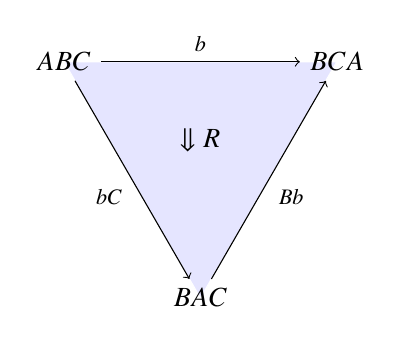
\begin{tikzpicture}
            \filldraw[white,fill=blue,fill opacity=0.1](30:2cm)--(150:2cm)--(270:2cm)--cycle;
            \node (A) at (30:2cm) {$BCA$};
            \node (C) at (150:2cm) {$ABC$}
              edge [->] node [l, above] {$b$} (A);
            \node (E) at (270:2cm) {$BAC$}
              edge [<-] node [l, below left] {$bC$} (C)
              edge [->] node [l, below right] {$Bb$} (A);
            \node at (0,0) {$\Downarrow R$};
          \end{tikzpicture}
          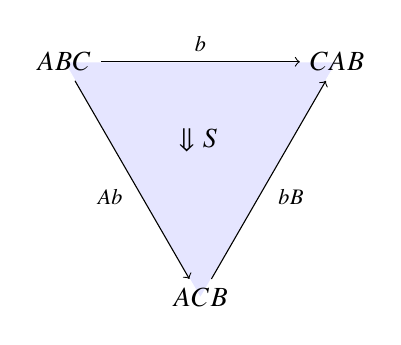
\begin{tikzpicture}
            \filldraw[white,fill=blue,fill opacity=0.1](30:2cm)--(150:2cm)--(270:2cm)--cycle;
            \node (A) at (30:2cm) {$CAB$};
            \node (C) at (150:2cm) {$ABC$}
              edge [->] node [l, above] {$b$} (A);
            \node (E) at (270:2cm) {$ACB$}
              edge [<-] node [l, below left] {$Ab$} (C)
              edge [->] node [l, below right] {$bB$} (A);
            \node at (0,0) {$\Downarrow S$};
          \end{tikzpicture}
        \end{center}
        When the associator is not the identity, the triangles' vertices get replaced with associators, effectively truncating them, and we are left with hexagon invertible modifications. (Mnemonic: Blue Braiding.)
        \begin{center}
          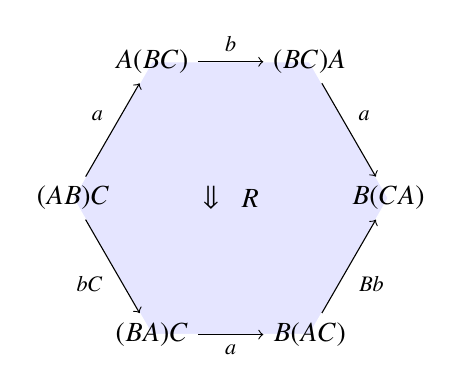
\begin{tikzpicture}
            \filldraw[white,fill=blue,fill opacity=0.1](0:2cm)--(60:2cm)--(120:2cm)--(180:2cm)--(240:2cm)--(300:2cm)--cycle;
            \node (A) at (  0:2cm) {$B(CA)$};
            \node (B) at ( 60:2cm) {$(BC)A$}
              edge [->] node [l, above right] {$a$} (A);
            \node (C) at (120:2cm) {$A(BC)$}
              edge [->] node [l, above] {$b$} (B);
            \node (D) at (180:2cm) {$(AB)C$}
              edge [->] node [l, above left] {$a$} (C);
            \node (E) at (240:2cm) {$(BA)C$}
              edge [<-] node [l, below left] {$bC$} (D);
            \node (F) at (300:2cm) {$B(AC)$}
              edge [<-] node [l, below] {$a$} (E)
              edge [->] node [l, below right] {$Bb$} (A);
            \node at (-0.25,0) {\tikz\node [rotate=-90] 
{$\Rightarrow$};};
            \node at (0.25,0) {$R$};
          \end{tikzpicture}
          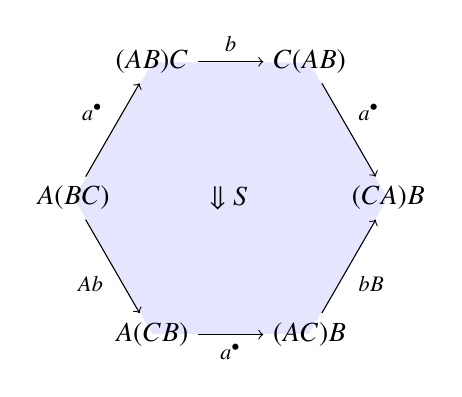
\begin{tikzpicture}
            \filldraw[white,fill=blue,fill opacity=0.1](0:2cm)--(60:2cm)--(120:2cm)--(180:2cm)--(240:2cm)--(300:2cm)--cycle;
            \node (A) at (  0:2cm) {$(CA)B$};
            \node (B) at ( 60:2cm) {$C(AB)$}
              edge [->] node [l, above right] {$a^\bullet$} (A);
            \node (C) at (120:2cm) {$(AB)C$}
              edge [->] node [l, above] {$b$} (B);
            \node (D) at (180:2cm) {$A(BC)$}
              edge [->] node [l, above left] {$a^\bullet$} (C);
            \node (E) at (240:2cm) {$A(CB)$}
              edge [<-] node [l, below left] {$Ab$} (D);
            \node (F) at (300:2cm) {$(AC)B$}
              edge [<-] node [l, below] {$a^\bullet$} (E)
              edge [->] node [l, below right] {$bB$} (A);
            \node at (0,0) {$\Downarrow S$};
          \end{tikzpicture}
        \end{center}
      \item $(n=3,k=1)$ and $(n=1,k=3)$: ${{3+1} \choose 1} = {{1+3}
\choose 1} = 4,$ so in a braided strictly monoidal bicategory, these polytopes are tetrahedra whose faces are the $(2,1)$ polytope.
        \begin{center}
          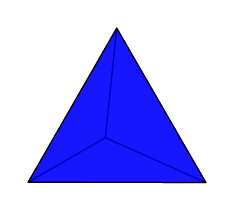
\begin{tikzpicture}[line join=round,scale=.2]
            \filldraw[fill=blue,fill opacity=0.7](-.551,-.318)--(.172,6.631)--(-5.449,-3.146)--cycle;
            \filldraw[fill=blue,fill opacity=0.7](-.551,-.318)--(5.828,-3.167)--(-5.449,-3.146)--cycle;
            \filldraw[fill=blue,fill opacity=0.7](-.551,-.318)--(.172,6.631)--(5.828,-3.167)--cycle;
            \filldraw[fill=blue,fill opacity=0.7](-5.449,-3.146)--(.172,6.631)--(5.828,-3.167)--cycle;
          \end{tikzpicture}% End sketch output
        \end{center}
        Again, when the associator is not the identity, the vertices get truncated, this time being replaced by pentagonators; as a side-effect, four of the six edges are also beveled.
        \begin{center}
          \begin{tikzpicture}[line join=round,scale=.2]
            \filldraw[fill=green,fill opacity=0.7](3.11,-1.226)--(1.675,-.585)--(1.112,-1.562)--(2.548,-2.203)--cycle;
            \filldraw[fill=blue,fill opacity=0.7](3.281,.425)--(2.009,2.629)--(-.144,3.591)--(-.235,2.722)--(1.675,-.585)--(3.11,-1.226)--cycle;
            \filldraw[fill=blue,fill opacity=0.7](-3.234,-1.214)--(-2.132,-.578)--(-.235,2.722)--(-.144,3.591)--(-1.798,2.636)--(-3.062,.436)--cycle;
            \filldraw[fill=red,fill opacity=0.7](-1.566,-1.557)--(-2.132,-.578)--(-.235,2.722)--(1.675,-.585)--(1.112,-1.562)--cycle;
            \filldraw[fill=blue,fill opacity=0.7](2.548,-2.203)--(1.112,-1.562)--(-1.566,-1.557)--(-2.668,-2.194)--(-.515,-3.155)--(.894,-3.158)--cycle;
            \filldraw[fill=green,fill opacity=0.7](-3.234,-1.214)--(-2.132,-.578)--(-1.566,-1.557)--(-2.668,-2.194)--cycle;
            \filldraw[fill=red,fill opacity=0.7](1.519,2.346)--(-1.16,2.351)--(-1.798,2.636)--(-.144,3.591)--(2.009,2.629)--cycle;
            \filldraw[fill=red,fill opacity=0.7](3.281,.425)--(2.791,.142)--(.894,-3.158)--(2.548,-2.203)--(3.11,-1.226)--cycle;
            \filldraw[fill=red,fill opacity=0.7](-3.234,-1.214)--(-2.668,-2.194)--(-.515,-3.155)--(-2.425,.152)--(-3.062,.436)--cycle;
            \filldraw[fill=green,fill opacity=0.7](3.281,.425)--(2.009,2.629)--(1.519,2.346)--(2.791,.142)--cycle;
            \filldraw[fill=green,fill opacity=0.7](-3.062,.436)--(-1.798,2.636)--(-1.16,2.351)--(-2.425,.152)--cycle;
            \filldraw[fill=blue,fill opacity=0.7](2.791,.142)--(1.519,2.346)--(-1.16,2.351)--(-2.425,.152)--(-.515,-3.155)--(.894,-3.158)--cycle;
          \end{tikzpicture}% End sketch output
        \end{center}
        This equation governs shuffling one object $A$ into three objects $B, C, D$: \\
        \begin{center}
          \begin{tikzpicture}[line join=round,scale=1.25]
            \filldraw[white,fill=red,fill opacity=0.1](1.519,2.346)--(-1.16,2.351)--(-1.798,2.636)--(-.144,3.591)--(2.009,2.629)--cycle;
            \filldraw[white,fill=red,fill opacity=0.1](3.281,.425)--(2.791,.142)--(.894,-3.158)--(2.548,-2.203)--(3.11,-1.226)--cycle;
            \filldraw[white,fill=red,fill opacity=0.1](-3.234,-1.214)--(-2.668,-2.194)--(-.515,-3.155)--(-2.425,.152)--(-3.062,.436)--cycle;
            \filldraw[white,fill=green,fill opacity=0.1](3.281,.425)--(2.009,2.629)--(1.519,2.346)--(2.791,.142)--cycle;
            \filldraw[white,fill=green,fill opacity=0.1](-3.062,.436)--(-1.798,2.636)--(-1.16,2.351)--(-2.425,.152)--cycle;
            \filldraw[white,fill=blue,fill opacity=0.1](2.791,.142)--(1.519,2.346)--(-1.16,2.351)--(-2.425,.152)--(-.515,-3.155)--(.894,-3.158)--cycle;
            \begin{scope}[font=\fontsize{8}{8}\selectfont]
              \node (A) at (-.144,3.591) {};
              \node[anchor=south] at (A) {$(A(BC))D$};
              \node (B) at (2.009,2.629) {}
                edge [<-] node [l, above right] {$a$} (A);
              \node[anchor=west] at (B) {$A((BC)D)$};
              \node (C) at (3.281,.425) {}
                edge [<-] node [l, above right] {$b$} (B);
              \node[anchor=west] at (C) {$((BC)D)A$};
              \node (D) at (3.11,-1.226) {}
                edge [<-] node [l, right] {$a$} (C);
              \node[anchor=west] at (D) {$(BC)(DA)$};
              \node (E) at (2.548,-2.203) {}
                edge [<-] node [l, right] {$a$} (D);
              \node[anchor=north west] at (E) {$B(C(DA))$};
              \node (F) at (.894,-3.158) {}
                edge [->] node [l, below right] {$Ba$} (E);
              \node[anchor=north] at (F) {$B((CD)A)$};
              \node (G) at (-.515,-3.155) {}
                edge [->] node [l, above] {$Bb$} (F);
              \node[anchor=north] at (G) {$B(A(CD))$};
              \node (H) at (-2.668,-2.194) {}
                edge [->] node [l, below left] {$Ba$} (G);
              \node[anchor=north east] at (H) {$B((AC)D)$};
              \node (I) at (-3.234,-1.214) {}
                edge [->] node [l, left] {$a$} (H);
              \node[anchor=east] at (I) {$(B(AC))D$};
              \node (J) at (-3.062,.436) {}
                edge [->] node [l, left] {$aD$} (I);
              \node[anchor=east] at (J) {$((BA)C)D$};
              \node (K) at (-1.798,2.636) {}
                edge [->] node [l, above left] {$(bC)D$} (J)
                edge [->] node [l, above left] {$aD$} (A);
              \node[anchor=east] at (K) {$((AB)C)D$};
              \node (L) at (-1.16,2.351) {}
                edge [<-] node [l, below left] {$a$} (K);
              \node[anchor=north west] at (L) {$(AB)(CD)$};
              \node (M) at (1.519,2.346) {}
                edge [<-] node [l, above] {$a$} (L)
                edge [<-] node [l, below, sloped] {$Aa$} (B);
              \node[anchor=north east] at (M) {$A(B(CD))$};
              \node (N) at (2.791,.142) {}
                edge [<-] node [l, left] {$b$} (M)
                edge [->] node [l, left] {$a$} (F)
                edge [<-] node [l, above, sloped] {$aA$} (C);
              \node[anchor=east] at (N) {$(B(CD))A$};
              \node (O) at (-2.425,.152) {}
                edge [<-] node [l, below right] {$b(CD)$} (L)
                edge [<-] node [l, above] {$a$} (J)
                edge [->] node [l, right] {$a$} (G);
              \node[anchor=west] at (O) {$(BA)(CD)$};
              \node at (-0.25,3) {\tikz\node [rotate=-90] 
{$\Rightarrow$};};
              \node at (0,3) {$\pi$};
              \node at (-2,1.5) {$\cong$};
              \node at (2.3,1.5) {$\cong$};
              \node at (-2.25,-1.5) {$\Leftarrow \pi^{-1}$};
              \node at (2.5,-1.5) {$\Leftarrow \pi^{-1}$};
              \node at (-0,0) {\tikz\node [rotate=-135] 
{$\Rightarrow$};};
              \node at (0.25,0) {$R$};
            \end{scope}
          \end{tikzpicture}% End sketch output
          \\
          =
          \\
          \begin{tikzpicture}[line join=round,scale=1.25]
            \filldraw[white,fill=green,fill opacity=0.1](3.11,-1.226)--(1.675,-.585)--(1.112,-1.562)--(2.548,-2.203)--cycle;
            \filldraw[white,fill=blue,fill opacity=0.1](3.281,.425)--(2.009,2.629)--(-.144,3.591)--(-.235,2.722)--(1.675,-.585)--(3.11,-1.226)--cycle;
            \filldraw[white,fill=blue,fill opacity=0.1](-3.234,-1.214)--(-2.132,-.578)--(-.235,2.722)--(-.144,3.591)--(-1.798,2.636)--(-3.062,.436)--cycle;
            \filldraw[white,fill=red,fill opacity=0.1](-1.566,-1.557)--(-2.132,-.578)--(-.235,2.722)--(1.675,-.585)--(1.112,-1.562)--cycle;
            \filldraw[white,fill=blue,fill opacity=0.1](2.548,-2.203)--(1.112,-1.562)--(-1.566,-1.557)--(-2.668,-2.194)--(-.515,-3.155)--(.894,-3.158)--cycle;
            \filldraw[white,fill=green,fill opacity=0.1](-3.234,-1.214)--(-2.132,-.578)--(-1.566,-1.557)--(-2.668,-2.194)--cycle;
            \begin{scope}[font=\fontsize{8}{8}\selectfont]
              \node (A) at (-.144,3.591) {};
              \node[anchor=south] at (A) {$(A(BC))D$};
              \node (B) at (2.009,2.629) {}
                edge [<-] node [l, above right] {$a$} (A);
              \node[anchor=west] at (B) {$A((BC)D)$};
              \node (C) at (3.281,.425) {}
                edge [<-] node [l, above right] {$b$} (B);
              \node[anchor=west] at (C) {$((BC)D)A$};
              \node (D) at (3.11,-1.226) {}
                edge [<-] node [l, right] {$a$} (C);
              \node[anchor=west] at (D) {$(BC)(DA)$};
              \node (E) at (2.548,-2.203) {}
                edge [<-] node [l, right] {$a$} (D);
              \node[anchor=north west] at (E) {$B(C(DA))$};
              \node (F) at (.894,-3.158) {}
                edge [->] node [l, below right] {$Ba$} (E);
              \node[anchor=north] at (F) {$B((CD)A)$};
              \node (G) at (-.515,-3.155) {}
                edge [->] node [l, above] {$Bb$} (F);
              \node[anchor=north] at (G) {$B(A(CD))$};
              \node (H) at (-2.668,-2.194) {}
                edge [->] node [l, below left] {$Ba$} (G);
              \node[anchor=north east] at (H) {$B((AC)D)$};
              \node (I) at (-3.234,-1.214) {}
                edge [->] node [l, left] {$a$} (H);
              \node[anchor=east] at (I) {$(B(AC))D$};
              \node (J) at (-3.062,.436) {}
                edge [->] node [l, left] {$aD$} (I);
              \node[anchor=east] at (J) {$((BA)C)D$};
              \node (K) at (-1.798,2.636) {}
                edge [->] node [l, above left] {$(bC)D$} (J)
                edge [->] node [l, above left] {$aD$} (A);
              \node[anchor=east] at (K) {$((AB)C)D$};
              \node (P) at (-2.132,-.578) {}
                edge [<-] node [l, above, sloped] {$(Bb)D$} (I);
              \node[anchor=west] at (P) {$(B(CA))D$};
              \node (Q) at (-.235,2.722) {}
                edge [->] node [l, below right] {$aD$} (P)
                edge [<-] node [l, left] {$bD$} (A);
              \node[anchor=west] at (Q) {$((BC)A)D$};
              \node (R) at (1.675,-.585) {}
                edge [<-] node [l, below left] {$a$} (Q)
                edge [->] node [l, above, sloped] {$(BC)b$} (D);
              \node[anchor=east] at (R) {$(BC)(AD)$};
              \node (S) at (1.112,-1.562) {}
                edge [<-] node [l, below right] {$a$} (R)
                edge [->] node [l, above, sloped] {$B(Cb)$} (E);
              \node[anchor=south east] at (S) {$B(C(AD))$};
              \node (T) at (-1.566,-1.557) {}
                edge [->] node [l, below] {$Ba$} (S)
                edge [<-] node [l, below left] {$a$} (P)
                edge [<-] node [l, above, sloped] {$B(bD)$} (H);
              \node[anchor=south west] at (T) {$B((CA)D)$};
              \node at (-0.25,0) {\tikz\node [rotate=-135] 
{$\Rightarrow$};};
              \node at (0.25,0) {$\pi^{-1}$};
              \node at (2,1) {$\Leftarrow R$};
              \node at (-2.25,1) {\tikz\node [rotate=-135] 
{$\Rightarrow$};};
              \node at (-2,1) {$RD$};
              \node at (2.25,-1.25) {$\cong$};
              \node at (-2.5,-1.25) {$\cong$};
              \node at (-0.5,-2.5) {\tikz\node [rotate=-90] 
{$\Rightarrow$};};
              \node at (0,-2.5) {$BR^{-1}$};
            \end{scope}
          \end{tikzpicture}% End sketch output
        \end{center}
        This equation governs shuffling one object $D$ into three objects $A,B,C$: \\
        \begin{center}
          \begin{tikzpicture}[line join=round,scale=1.25]
            \filldraw[white,fill=red,fill opacity=0.1](1.519,2.346)--(-1.16,2.351)--(-1.798,2.636)--(-.144,3.591)--(2.009,2.629)--cycle;
            \filldraw[white,fill=red,fill opacity=0.1](3.281,.425)--(2.791,.142)--(.894,-3.158)--(2.548,-2.203)--(3.11,-1.226)--cycle;
            \filldraw[white,fill=red,fill opacity=0.1](-3.234,-1.214)--(-2.668,-2.194)--(-.515,-3.155)--(-2.425,.152)--(-3.062,.436)--cycle;
            \filldraw[white,fill=green,fill opacity=0.1](3.281,.425)--(2.009,2.629)--(1.519,2.346)--(2.791,.142)--cycle;
            \filldraw[white,fill=green,fill opacity=0.1](-3.062,.436)--(-1.798,2.636)--(-1.16,2.351)--(-2.425,.152)--cycle;
            \filldraw[white,fill=blue,fill opacity=0.1](2.791,.142)--(1.519,2.346)--(-1.16,2.351)--(-2.425,.152)--(-.515,-3.155)--(.894,-3.158)--cycle;
            \begin{scope}[font=\fontsize{8}{8}\selectfont]
              \node (A) at (-.144,3.591) {};
              \node[anchor=south] at (A) {$A((BC)D)$};
              \node (B) at (2.009,2.629) {}
                edge [<-] node [l, above right] {$a^\bullet$} (A);
              \node[anchor=west] at (B) {$(A(BC))D$};
              \node (C) at (3.281,.425) {}
                edge [<-] node [l, above right] {$b$} (B);
              \node[anchor=west] at (C) {$D(A(BC))$};
              \node (D) at (3.11,-1.226) {}
                edge [<-] node [l, right] {$a^\bullet$} (C);
              \node[anchor=west] at (D) {$(DA)(BC)$};
              \node (E) at (2.548,-2.203) {}
                edge [<-] node [l, right] {$a^\bullet$} (D);
              \node[anchor=north west] at (E) {$((DA)B)C$};
              \node (F) at (.894,-3.158) {}
                edge [->] node [l, below right] {$a^\bullet C$} (E);
              \node[anchor=north] at (F) {$(D(AB))C$};
              \node (G) at (-.515,-3.155) {}
                edge [->] node [l, above] {$bC$} (F);
              \node[anchor=north] at (G) {$((AB)D)C$};
              \node (H) at (-2.668,-2.194) {}
                edge [->] node [l, below left] {$a^\bullet C$} (G);
              \node[anchor=north east] at (H) {$(A(BD))C$};
              \node (I) at (-3.234,-1.214) {}
                edge [->] node [l, left] {$a^\bullet$} (H);
              \node[anchor=east] at (I) {$A((BD)C)$};
              \node (J) at (-3.062,.436) {}
                edge [->] node [l, left] {$Aa^\bullet$} (I);
              \node[anchor=east] at (J) {$A(B(DC))$};
              \node (K) at (-1.798,2.636) {}
                edge [->] node [l, above left] {$a(Bb)$} (J)
                edge [->] node [l, above left] {$Aa^\bullet$} (A);
              \node[anchor=east] at (K) {$A(B(CD))$};
              \node (L) at (-1.16,2.351) {}
                edge [<-] node [l, below left] {$a^\bullet$} (K);
              \node[anchor=north west] at (L) {$(AB)(CD)$};
              \node (M) at (1.519,2.346) {}
                edge [<-] node [l, above] {$a^\bullet$} (L)
                edge [<-] node [l, below, sloped] {$a^\bullet D$} (B);
              \node[anchor=north east] at (M) {$((AB)C)D$};
              \node (N) at (2.791,.142) {}
                edge [<-] node [l, left] {$b$} (M)
                edge [->] node [l, left] {$a^\bullet$} (F)
                edge [<-] node [l, above, sloped] {$Da^\bullet$} (C);
              \node[anchor=east] at (N) {$D((AB)C)$};
              \node (O) at (-2.425,.152) {}
                edge [<-] node [l, below right] {$(AB)b$} (L)
                edge [<-] node [l, above] {$a^\bullet$} (J)
                edge [->] node [l, right] {$a^\bullet$} (G);
              \node[anchor=west] at (O) {$(AB)(DC)$};
              \node at (-0.25,3) {\tikz\node [rotate=-90] 
{$\Rightarrow$};};
              \node at (0,3) {$\pi^\bullet$};
              \node at (-2,1.5) {$\cong$};
              \node at (2.3,1.5) {$\cong$};
              \node at (-2.25,-1.5) {$\Leftarrow \pi^{\bullet-1}$};
              \node at (2.5,-1.5) {$\Leftarrow \pi^{\bullet-1}$};
              \node at (-0,0) {\tikz\node [rotate=-135] 
{$\Rightarrow$};};
              \node at (0.25,0) {$S$};
            \end{scope}
          \end{tikzpicture}% End sketch output
          \\
          =
          \\
          \begin{tikzpicture}[line join=round,scale=1.25]
            \filldraw[white,fill=green,fill opacity=0.1](3.11,-1.226)--(1.675,-.585)--(1.112,-1.562)--(2.548,-2.203)--cycle;
            \filldraw[white,fill=blue,fill opacity=0.1](3.281,.425)--(2.009,2.629)--(-.144,3.591)--(-.235,2.722)--(1.675,-.585)--(3.11,-1.226)--cycle;
            \filldraw[white,fill=blue,fill opacity=0.1](-3.234,-1.214)--(-2.132,-.578)--(-.235,2.722)--(-.144,3.591)--(-1.798,2.636)--(-3.062,.436)--cycle;
            \filldraw[white,fill=red,fill opacity=0.1](-1.566,-1.557)--(-2.132,-.578)--(-.235,2.722)--(1.675,-.585)--(1.112,-1.562)--cycle;
            \filldraw[white,fill=blue,fill opacity=0.1](2.548,-2.203)--(1.112,-1.562)--(-1.566,-1.557)--(-2.668,-2.194)--(-.515,-3.155)--(.894,-3.158)--cycle;
            \filldraw[white,fill=green,fill opacity=0.1](-3.234,-1.214)--(-2.132,-.578)--(-1.566,-1.557)--(-2.668,-2.194)--cycle;
            \begin{scope}[font=\fontsize{8}{8}\selectfont]
              \node (A) at (-.144,3.591) {};
              \node[anchor=south] at (A) {$A((BC)D)$};
              \node (B) at (2.009,2.629) {}
                edge [<-] node [l, above right] {$a^\bullet$} (A);
              \node[anchor=west] at (B) {$(A(BC))D$};
              \node (C) at (3.281,.425) {}
                edge [<-] node [l, above right] {$b$} (B);
              \node[anchor=west] at (C) {$D(A(BC))$};
              \node (D) at (3.11,-1.226) {}
                edge [<-] node [l, right] {$a^\bullet$} (C);
              \node[anchor=west] at (D) {$(DA)(BC)$};
              \node (E) at (2.548,-2.203) {}
                edge [<-] node [l, right] {$a^\bullet$} (D);
              \node[anchor=north west] at (E) {$((DA)B)C$};
              \node (F) at (.894,-3.158) {}
                edge [->] node [l, below right] {$a^\bullet C$} (E);
              \node[anchor=north] at (F) {$(D(AB))C$};
              \node (G) at (-.515,-3.155) {}
                edge [->] node [l, above] {$bC$} (F);
              \node[anchor=north] at (G) {$((AB)D)C$};
              \node (H) at (-2.668,-2.194) {}
                edge [->] node [l, below left] {$a^\bullet C$} (G);
              \node[anchor=north east] at (H) {$(A(BD))C$};
              \node (I) at (-3.234,-1.214) {}
                edge [->] node [l, left] {$a^\bullet$} (H);
              \node[anchor=east] at (I) {$A((BD)C)$};
              \node (J) at (-3.062,.436) {}
                edge [->] node [l, left] {$Aa^\bullet$} (I);
              \node[anchor=east] at (J) {$A(B(DC))$};
              \node (K) at (-1.798,2.636) {}
                edge [->] node [l, above left] {$A(Bb)$} (J)
                edge [->] node [l, above left] {$Aa^\bullet$} (A);
              \node[anchor=east] at (K) {$A(B(CD))$};
              \node (P) at (-2.132,-.578) {}
                edge [<-] node [l, above, sloped] {$A(bC)$} (I);
              \node[anchor=west] at (P) {$A((DB)C)$};
              \node (Q) at (-.235,2.722) {}
                edge [->] node [l, below right] {$Aa^\bullet$} (P)
                edge [<-] node [l, left] {$Ab$} (A);
              \node[anchor=west] at (Q) {$A(D(BC))$};
              \node (R) at (1.675,-.585) {}
                edge [<-] node [l, below left] {$a^\bullet$} (Q)
                edge [->] node [l, above, sloped] {$b(BC)$} (D);
              \node[anchor=east] at (R) {$(AD)(BC)$};
              \node (S) at (1.112,-1.562) {}
                edge [<-] node [l, below right] {$a^\bullet$} (R)
                edge [->] node [l, above, sloped] {$(bB)C$} (E);
              \node[anchor=south east] at (S) {$((AD)B)C$};
              \node (T) at (-1.566,-1.557) {}
                edge [->] node [l, below] {$a^\bullet C$} (S)
                edge [<-] node [l, below left] {$a^\bullet$} (P)
                edge [<-] node [l, above, sloped] {$(Ab)C$} (H);
              \node[anchor=south west] at (T) {$(A(DB))C$};
              \node at (-0.25,0) {\tikz\node [rotate=-135] 
{$\Rightarrow$};};
              \node at (0.25,0) {$\pi^{\bullet-1}$};
              \node at (2,1) {$\Leftarrow S$};
              \node at (-2.25,1) {\tikz\node [rotate=-135] 
{$\Rightarrow$};};
              \node at (-2,1) {$AS$};
              \node at (2.25,-1.25) {$\cong$};
              \node at (-2.5,-1.25) {$\cong$};
              \node at (-0.5,-2.5) {\tikz\node [rotate=-90] 
{$\Rightarrow$};};
              \node at (0,-2.5) {$S^{-1}C$};
            \end{scope}
          \end{tikzpicture}% End sketch output
        \end{center}
        
      \item $(n=2,k=2)$: ${{2+2} \choose 2} = 6;$ in a braided strictly monoidal bicategory, this polytope is composed mostly of (2,1) triangles, but there is a pair of braidings that commute, so one face is a square.
        \begin{center}
          \begin{tikzpicture}[line join=round, scale=.5]
            \filldraw[fill=blue,fill opacity=0.7](-5.635,-.347)--(-1.888,.116)--(0,-1.695)--cycle;
            \filldraw[fill=blue,fill opacity=0.7](5.635,-.347)--(0,-1.695)--(1.888,.116)--cycle;
            \filldraw[fill=green,fill opacity=0.7](0,2.083)--(-1.888,.116)--(0,-1.695)--(1.888,.116)--cycle;
            \filldraw[fill=blue,fill opacity=0.7](5.635,-.347)--(-5.635,-.347)--(0,-1.695)--cycle;
            \filldraw[fill=blue,fill opacity=0.7](5.635,-.347)--(1.888,.116)--(0,2.083)--cycle;
            \filldraw[fill=blue,fill opacity=0.7](0,2.083)--(-1.888,.116)--(-5.635,-.347)--cycle;
            \filldraw[fill=blue,fill opacity=0.7](5.635,-.347)--(-5.635,-.347)--(0,2.083)--cycle;
          \end{tikzpicture}% End sketch output
        \end{center}
        When the associator is not the identity, the six vertices get truncated and six of the edges get beveled.
        \begin{center}
          \begin{tikzpicture}[line join=round, scale=.5]
            \filldraw[fill=green,fill opacity=0.7](0,-.807)--(-.944,.116)--(-1.678,-.488)--(-.546,-1.564)--cycle;
            \filldraw[fill=green,fill opacity=0.7](.944,.116)--(0,-.807)--(.546,-1.564)--(1.678,-.488)--cycle;
            \filldraw[fill=green,fill opacity=0.7](.944,.116)--(0,-.807)--(-.944,.116)--(0,1.079)--cycle;
            \filldraw[fill=red,fill opacity=0.7](.546,-1.564)--(.453,-1.75)--(-.453,-1.75)--(-.546,-1.564)--(0,-.807)--cycle;
            \filldraw[fill=green,fill opacity=0.7](0,1.079)--(-.944,.116)--(-1.72,.642)--(-.588,1.829)--cycle;
            \filldraw[fill=green,fill opacity=0.7](.944,.116)--(0,1.079)--(.588,1.829)--(1.72,.642)--cycle;
            \filldraw[fill=red,fill opacity=0.7](1.678,-.488)--(2.075,-.32)--(2.109,.417)--(1.72,.642)--(.944,.116)--cycle;
            \filldraw[fill=red,fill opacity=0.7](-1.72,.642)--(-2.109,.417)--(-2.075,-.32)--(-1.678,-.488)--(-.944,.116)--cycle;
            \filldraw[fill=red,fill opacity=0.7](.588,1.829)--(.492,2.021)--(-.492,2.021)--(-.588,1.829)--(0,1.079)--cycle;
            \filldraw[fill=blue,fill opacity=0.7](1.678,-.488)--(2.075,-.32)--(2.573,-.48)--(2.308,-.977)--(.453,-1.75)--(.546,-1.564)--cycle;
            \filldraw[fill=blue,fill opacity=0.7](-.546,-1.564)--(-.453,-1.75)--(-2.308,-.977)--(-2.573,-.48)--(-2.075,-.32)--(-1.678,-.488)--cycle;
            \filldraw[fill=blue,fill opacity=0.7](-.453,-1.75)--(-2.308,-.977)--(-1.412,-.174)--(1.412,-.174)--(2.308,-.977)--(.453,-1.75)--cycle;
            \filldraw[fill=blue,fill opacity=0.7](1.72,.642)--(.588,1.829)--(.492,2.021)--(2.405,.899)--(2.625,.433)--(2.109,.417)--cycle;
            \filldraw[fill=blue,fill opacity=0.7](-.588,1.829)--(-.492,2.021)--(-2.405,.899)--(-2.625,.433)--(-2.109,.417)--(-1.72,.642)--cycle;
            \filldraw[fill=green,fill opacity=0.7](2.075,-.32)--(2.573,-.48)--(2.625,.433)--(2.109,.417)--cycle;
            \filldraw[fill=green,fill opacity=0.7](-2.075,-.32)--(-2.573,-.48)--(-2.625,.433)--(-2.109,.417)--cycle;
            \filldraw[fill=blue,fill opacity=0.7](.492,2.021)--(-.492,2.021)--(-2.405,.899)--(-1.412,-.174)--(1.412,-.174)--(2.405,.899)--cycle;
            \filldraw[fill=red,fill opacity=0.7](2.625,.433)--(2.405,.899)--(1.412,-.174)--(2.308,-.977)--(2.573,-.48)--cycle;
            \filldraw[fill=red,fill opacity=0.7](-2.625,.433)--(-2.405,.899)--(-1.412,-.174)--(-2.308,-.977)--(-2.573,-.48)--cycle;
          \end{tikzpicture}% End sketch output
        \end{center}
        This equation governs shuffling two objects $A, B$ into two objects $C, D$: \\
        \begin{center}
          \begin{tikzpicture}[line join=round, scale=2.5, font=\fontsize
{5}{5}\selectfont]
            \filldraw[white,fill=blue,fill opacity=0.1](-.453,-1.75)--(-2.308,-.977)--(-1.412,-.174)--(1.412,-.174)--(2.308,-.977)--(.453,-1.75)--cycle;
            \filldraw[white,fill=blue,fill opacity=0.1](.492,2.021)--(-.492,2.021)--(-2.405,.899)--(-1.412,-.174)--(1.412,-.174)--(2.405,.899)--cycle;
            \filldraw[white,fill=red,fill opacity=0.1](2.625,.433)--(2.405,.899)--(1.412,-.174)--(2.308,-.977)--(2.573,-.48)--cycle;
            \filldraw[white,fill=red,fill opacity=0.1](-2.625,.433)--(-2.405,.899)--(-1.412,-.174)--(-2.308,-.977)--(-2.573,-.48)--cycle;
            \node (A) at (-2.573,-.48) {};
            \node [left] at (A) {$(A(BC))D$};

            \node (B) at (-2.625,.433) {}
              edge [<-] node [l, left] {$a$} (A);
            \node [left] at (B) {$A((BC)D)$};

            \node (C) at (-2.405,.899) {}
              edge [<-] node [l, left] {$Aa$} (B);
            \node [left] at (C) {$A(B(CD))$};

            \node (D) at (-.492,2.021) {}
              edge [<-] node [l, above left] {$Ab$} (C);
            \node [above] at (D) {$A((CD)B)$};

            \node (E) at (.492,2.021) {}
              edge [<-] node [l, above] {$a^\bullet$} (D);
            \node [above] at (E) {$(A(CD))B$};

            \node (F) at (2.405,.899) {}
              edge [<-] node [l, above right] {$bB$} (E);
            \node [right] at (F) {$((CD)A)B$};

            \node (G) at (2.625,.433) {}
              edge [<-] node [l, right] {$aB$} (F);
            \node [right] at (G) {$(C(DA))B$};

            \node (H) at (2.573,-.48) {}
              edge [<-] node [l, right] {$a$} (G);
            \node [right] at (H) {$C((DA)B)$};

            \node (I) at (2.308,-.977) {}
              edge [->] node [l, right] {$Ca^\bullet$} (H);
            \node [right] at (I) {$C(D(AB))$};

            \node (J) at (.453,-1.75) {}
              edge [->] node [l, below right] {$Cb$} (I);
            \node [below] at (J) {$C((AB)D)$};

            \node (K) at (-.453,-1.75) {}
              edge [->] node [l, below] {$a$} (J);
            \node [below] at (K) {$(C(AB))D$};

            \node (L) at (-2.308,-.977) {}
              edge [->] node [l, below left] {$bD$} (K)
              edge [<-] node [l, left] {$a^\bullet D$} (A);
            \node [left] at (L) {$((AB)C)D$};

            \node (M) at (-1.412,-.174) {$(AB)(CD)$}
              edge [<-] node [l, below right] {$a$} (L)
              edge [<-] node [l, above right] {$a^\bullet$} (C);

            \node (N) at (1.412,-.174) {$(CD)(AB)$}
              edge [<-] node [l, above] {$b$} (M)
              edge [->] node [l, below left] {$a$} (I)
              edge [->] node [l, above left] {$a^\bullet$} (F);
            \begin{scope}[font=\fontsize{10}{10}\selectfont]
              \node at (-2.2,0) {$\Uparrow \pi_1$};
              \node at (0,1) {$\Uparrow S$};
              \node at (0,-1) {$\Uparrow R^{-1}$};
              \node at (2.2,0) {$\Uparrow \pi_2$};
            \end{scope}
          \end{tikzpicture}% End sketch output
          \\ = \\
          \begin{tikzpicture}[line join=round, scale=2.5, font=\fontsize
{5}{5}\selectfont]
            \filldraw[white,fill=green,fill opacity=0.1](0,-.807)--(-.944,.116)--(-1.678,-.488)--(-.546,-1.564)--cycle;
            \filldraw[white,fill=green,fill opacity=0.1](.944,.116)--(0,-.807)--(.546,-1.564)--(1.678,-.488)--cycle;
            \filldraw[white,fill=green,fill opacity=0.1](.944,.116)--(0,-.807)--(-.944,.116)--(0,1.079)--cycle;
            \filldraw[white,fill=red,fill opacity=0.1](.546,-1.564)--(.453,-1.75)--(-.453,-1.75)--(-.546,-1.564)--(0,-.807)--cycle;
            \filldraw[white,fill=green,fill opacity=0.1](0,1.079)--(-.944,.116)--(-1.72,.642)--(-.588,1.829)--cycle;
            \filldraw[white,fill=green,fill opacity=0.1](.944,.116)--(0,1.079)--(.588,1.829)--(1.72,.642)--cycle;
            \filldraw[white,fill=red,fill opacity=0.1](1.678,-.488)--(2.075,-.32)--(2.109,.417)--(1.72,.642)--(.944,.116)--cycle;
            \filldraw[white,fill=red,fill opacity=0.1](-1.72,.642)--(-2.109,.417)--(-2.075,-.32)--(-1.678,-.488)--(-.944,.116)--cycle;
            \filldraw[white,fill=red,fill opacity=0.1](.588,1.829)--(.492,2.021)--(-.492,2.021)--(-.588,1.829)--(0,1.079)--cycle;
            \filldraw[white,fill=blue,fill opacity=0.1](1.678,-.488)--(2.075,-.32)--(2.573,-.48)--(2.308,-.977)--(.453,-1.75)--(.546,-1.564)--cycle;
            \filldraw[white,fill=blue,fill opacity=0.1](-.546,-1.564)--(-.453,-1.75)--(-2.308,-.977)--(-2.573,-.48)--(-2.075,-.32)--(-1.678,-.488)--cycle;
            \filldraw[white,fill=blue,fill opacity=0.1](1.72,.642)--(.588,1.829)--(.492,2.021)--(2.405,.899)--(2.625,.433)--(2.109,.417)--cycle;
            \filldraw[white,fill=blue,fill opacity=0.1](-.588,1.829)--(-.492,2.021)--(-2.405,.899)--(-2.625,.433)--(-2.109,.417)--(-1.72,.642)--cycle;
            \filldraw[white,fill=green,fill opacity=0.1](2.075,-.32)--(2.573,-.48)--(2.625,.433)--(2.109,.417)--cycle;
            \filldraw[white,fill=green,fill opacity=0.1](-2.075,-.32)--(-2.573,-.48)--(-2.625,.433)--(-2.109,.417)--cycle;

            \node (A) at (-2.573,-.48) {};
            \node [left] at (A) {$(A(BC))D$};

            \node (B) at (-2.625,.433) {}
              edge [<-] node [l, left] {$a$} (A);
            \node [left] at (B) {$A((BC)D)$};

            \node (C) at (-2.405,.899) {}
              edge [<-] node [l, left] {$Aa$} (B);
            \node [left] at (C) {$A(B(CD))$};

            \node (D) at (-.492,2.021) {}
              edge [<-] node [l, above left] {$Ab$} (C);
            \node [above] at (D) {$A((CD)B)$};

            \node (E) at (.492,2.021) {}
              edge [<-] node [l, above] {$a^\bullet$} (D);
            \node [above] at (E) {$(A(CD))B$};

            \node (F) at (2.405,.899) {}
              edge [<-] node [l, above right] {$bB$} (E);
            \node [right] at (F) {$((CD)A)B$};

            \node (G) at (2.625,.433) {}
              edge [<-] node [l, right] {$aB$} (F);
            \node [right] at (G) {$(C(DA))B$};

            \node (H) at (2.573,-.48) {}
              edge [<-] node [l, right] {$a$} (G);
            \node [right] at (H) {$C((DA)B)$};

            \node (I) at (2.308,-.977) {}
              edge [->] node [l, right] {$Ca^\bullet$} (H);
            \node [right] at (I) {$C(D(AB))$};

            \node (J) at (.453,-1.75) {}
              edge [->] node [l, below right] {$Cb$} (I);
            \node [below] at (J) {$C((AB)D)$};

            \node (K) at (-.453,-1.75) {}
              edge [->] node [l, below] {$a$} (J);
            \node [below] at (K) {$(C(AB))D$};

            \node (L) at (-2.308,-.977) {}
              edge [->] node [l, below left] {$bD$} (K)
              edge [<-] node [l, left] {$a^\bullet D$} (A);
            \node [left] at (L) {$((AB)C)D$};

            \node (O) at (-2.075,-.32) {}
              edge [<-] node [l, below, sloped] {$(Ab)D$} (A);
            \node [above right] at (O) {$(A(CB))D$};

            \node (P) at (-2.109,.417) {}
              edge [<-] node [l, left] {$a$} (O)
              edge [<-] node [l, above, sloped] {$A(bD)$} (B);
            \node [below right] at (P) {$A((BC)D)$};

            \node (Q) at (-1.72,.642) {}
              edge [<-] node [l, above, sloped] {$Aa$} (P);
            \node [right] at (Q) {$A(C(BD))$};

            \node (R) at (-.944,.116) {$(AC)(BD)$}
              edge [<-] node [l, above right] {$a^\bullet$} (Q);

            \node (S) at (-1.678,-.488) {}
              edge [->] node [l, below right] {$a$} (R)
              edge [<-] node [l, below, sloped] {$a^\bullet D$} (O);
            \node [right] at (S) {$((AC)B)D$};

            \node (T) at (-.546,-1.564) {}
              edge [<-] node [l, above, sloped] {$(bB)D$} (S)
              edge [<-] node [right] {$a^\bullet D$} (K);
            \node at (T) {$((CA)B)D$};

            \node (U) at (0,-.807) {$(CA)(BD)$}
              edge [<-] node [l, above left] {$a$} (T)
              edge [<-] node [l, above, sloped] {$b(BD)$} (R);

            \node (V) at (.546,-1.564) {}
              edge [<-] node [l, above right] {$a$} (U)
              edge [->] node [left] {$Ca^\bullet$} (J);
            \node at (V) {$C(A(BD))$};

            \node (W) at (1.678,-.488) {}
              edge [<-] node [l, above, sloped] {$C(Ab)$} (V);
            \node [left] at (W) {$C(A(DB))$};

            \node (X) at (2.075,-.32) {}
              edge [<-] node [l, below, sloped] {$Ca^\bullet$} (W)
              edge [->] node [l, below, sloped] {$C(bB)$} (H);
            \node [above left] at (X) {$C((AD)B)$};

            \node (Y) at (2.109,.417) {}
              edge [->] node [l, right] {$a$} (X)
              edge [->] node [l, above, sloped] {$(Cb)B$} (G);
            \node [below left] at (Y) {$(C(AD))B$};

            \node (Z) at (1.72,.642) {}
              edge [->] node [l, above, sloped] {$aB$} (Y);
            \node [left] at (Z) {$((CA)D)B$};

            \node (A') at (.944,.116) {$(CA)(DB)$}
              edge [->] node [l, above left] {$a^\bullet$} (Z)
              edge [->] node [l, below left] {$a$} (W)
              edge [<-] node [l, above, sloped] {$(CA)b$} (U);

            \node (B') at (0,1.079) {$(AC)(DB)$}
              edge [->] node [l, below, sloped] {$b(DB)$} (A')
              edge [<-] node [l, below, sloped] {$(AC)b$} (R);

            \node (C') at (-.588,1.829) {}
              edge [->] node [l, below left] {$a^\bullet$} (B')
              edge [<-] node [l, below, sloped] {$A(Cb)$} (Q)
              edge [<-] node [right] {$Aa$} (D);
            \node at (C') {$A(C(DB))$};

            \node (D') at (.588,1.829) {}
              edge [<-] node [l, below right] {$a^\bullet$} (B')
              edge [->] node [l, below, sloped] {$(bD)B$} (Z)
              edge [->] node [left] {$aB$} (E);
            \node at (D') {$((AC)D)B$};

            \begin{scope} [font=\fontsize{10}{10}\selectfont]
              \node at (-2.4,0) {$\cong$};
              \node at (-1.7,0) {\tikz\node [rotate=90] 
{$\Rightarrow$};};
              \node at (-1.5,0) {$\pi_1$};
              \node at (-2,-.8) {\tikz\node [rotate=90] 
{$\Rightarrow$};};
              \node at (-1.8,-.8) {$SD$};
              \node at (-2,.9) {\tikz\node [rotate=90] 
{$\Rightarrow$};};
              \node at (-1.75,.9) {$AR^{-1}$};
              \node at (-0.1,1.6) {\tikz\node [rotate=90] 
{$\Rightarrow$};};
              \node at (0.1,1.6) {$\pi_4$};
              \node at (-.75,.75) {$\cong$};
              \node at (-.75,-.75) {$\cong$};
              \node at (0,0) {$\cong$};
              \node at (.75,-.75) {$\cong$};
              \node at (.75,.75) {$\cong$};
              \node at (-0.1,-1.5) {\tikz\node [rotate=90] 
{$\Rightarrow$};};
              \node at (0.1,-1.5) {$\pi_3$};
              \node at (1.8,.9) {\tikz\node [rotate=90] 
{$\Rightarrow$};};
              \node at (2.05,.9) {$R^{-1}B$};
              \node at (1.8,-.8) {\tikz\node [rotate=90] 
{$\Rightarrow$};};
              \node at (2, -.8) {$CS$};
              \node at (1.5,0) {\tikz\node [rotate=90] 
{$\Rightarrow$};};
              \node at (1.7,0) {$\pi_2$};
              \node at (2.4,0) {$\cong$};
            \end{scope}
          \end{tikzpicture}% End sketch output
        \end{center}
    \end{itemize}
    \item The Breen polytope.  In a braided monoidal category, the Yang-Baxter equations hold; there are two fundamentally distinct proofs of this fact.
    \begin{center}
      \begin{tikzpicture}
        \begin{scope}[scale=.3, font=\fontsize{8}{8}\selectfont]
          \node (ACB) at (5,0) {ACB};
          \node (ABC) at (0,3) {ABC}
            edge [->] node [l, below left] {$Ab$} (ACB);
          \node (CAB) at (10,3) {CAB}
            edge [<-] node [l, below right] {$b B$} (ACB);
          \node (BAC) at (0,9) {BAC}
            edge [<-] node [l, left] {$b C$} (ABC);
          \node (CBA) at (10,9) {CBA}
            edge [<-] node [l, above left] {$b$} (ACB)
            edge [<-] node [l, right] {$Cb$} (CAB);
          \node (BCA) at (5,12) {BCA}
            edge [<-] node [l, above left] {$Bb$} (BAC)
            edge [<-] node [l, below right] {$b$} (ABC)
            edge [->] node [l, above right] {$b A$} (CBA);
        \end{scope}
      \end{tikzpicture}
      \begin{tikzpicture}
        \begin{scope}[scale=.3, font=\fontsize{8}{8}\selectfont]
          \node (ACB) at (5,0) {ACB};
          \node (ABC) at (0,3) {ABC}
            edge [->] node [l, below left] {$Ab$} (ACB);
          \node (CAB) at (10,3) {CAB}
            edge [<-] node [l, above] {$b$} (ABC)
            edge [<-] node [l, below right] {$b B$} (ACB);
          \node (BAC) at (0,9) {BAC}
            edge [<-] node [l, left] {$b C$} (ABC);
          \node (CBA) at (10,9) {CBA}
            edge [<-] node [l, below] {$b$} (BAC)
            edge [<-] node [l, right] {$Cb$} (CAB);
          \node (BCA) at (5,12) {BCA}
            edge [<-] node [l, above left] {$Bb$} (BAC)
            edge [->] node [l, above right] {$b A$} (CBA);
        \end{scope}
      \end{tikzpicture}
    \end{center}
    In a braided strictly monoidal bicategory, the two proofs become the front and back face of another coherence law governing the interaction of the (2,1)-shuffle polytopes; when the associator is nontrivial, the vertices get truncated.  That the coherence law is necessary was something of a surprise: Kapranov and Voevodsky did not include it in their definition of braided semistrict monoidal 2-categories; Breen
\cite{Breen} corrected the definition.  We therefore call the following coherence law the ``Breen polytope''.  In retrospect, we can see that this is the start of a series of polytopes whose faces are
``permutohedra'' \cite{Permutohedra}; the need for the Breen polytope and the rest of the series became clear in Batanin's approach to weak 
$n$-categories \cite{Batanin}.
    \begin{center}
      \begin{tikzpicture}
        \begin{scope}[scale=.8, font=\fontsize{8}{8}\selectfont]
          \filldraw[white,fill=blue,fill opacity=0.1] (1,2.5)--(0,4)--(0,8)--(1,9.5)--(4,11.5)--(6,11.5)--cycle;
          \filldraw[white,fill=blue,fill opacity=0.1] (9,9.5)--(10,8)--(10,4)--(9,2.5)--(6,0.5)--(4,0.5)--cycle;
          \filldraw[white,fill=green,fill opacity=0.1] (6,11.5)--(9,9.5)--(4,0.5)--(1,2.5)--cycle;
          \node (ABC1) at (1, 2.5) {};
          \node [below left, l] at (ABC1) {$A(BC)$};
          \node (ABC2) at (0, 4) {}
            edge [<-] node [below left, l] {$a^\bullet$} (ABC1);
          \node [left, l] at (ABC2) {$(AB)C$};
          \node (BAC1) at (0, 8) {}
            edge [<-] node [left, l] {$bC$} (ABC2);
          \node [left, l] at (BAC1) {$(BA)C$};
          \node (BAC2) at (1, 9.5) {}
            edge [<-] node [left, l] {$a$} (BAC1);
          \node [above left, l] at (BAC2) {$B(AC)$};
          \node (BCA1) at (4, 11.5) {}
            edge [<-] node [above left, l] {$Bb$} (BAC2);
          \node [above, l] at (BCA1) {$B(CA)$};
          \node (BCA2) at (6, 11.5) {}
            edge [<-] node [above, l] {$a^\bullet$} (BCA1)
            edge [<-] node [below right] {$b$} (ABC1);
          \node [above, l] at (BCA2) {$(BC)A$};
          \node (CBA1) at (9, 9.5) {}
            edge [<-] node [above right, l] {$bA$} (BCA2);
          \node [above right, l] at (CBA1) {$(CB)A$};
          \node (CBA2) at (10, 8) {}
            edge [->] node [right, l] {$a^\bullet$} (CBA1);
          \node [right, l] at (CBA2) {$C(BA)$};
          \node (CAB1) at (10, 4) {}
            edge [->] node [right, l] {$Cb$} (CBA2);
          \node [right, l] at (CAB1) {$C(AB)$};
          \node (CAB2) at (9, 2.5) {}
            edge [->] node [right, l] {$a$} (CAB1);
          \node [below right, l] at (CAB2) {$(CA)B$};
          \node (ACB1) at (6, 0.5) {}
            edge [->] node [below right, l] {$bB$} (CAB2);
          \node [below, l] at (ACB1) {$(AC)B$};
          \node (ACB2) at (4, 0.5) {}
            edge [->] node [below, l] {$a^\bullet$} (ACB1)
            edge [->] node [below right, l] {$b$} (CBA1)
            edge [<-] node [below left, l] {$Ab$} (ABC1);
          \node [below, l] at (ACB2) {$A(CB)$};
          \node at (2, 7.5) {$\Rightarrow R_1^{-1}$};
          \node at (5, 6) {$\cong$};
          \node at (8, 4.5) {$\Rightarrow R_1$};
        \end{scope}
      \end{tikzpicture}
      \\ = \\
      \begin{tikzpicture}
        \begin{scope}[scale=.8, font=\fontsize{8}{8}\selectfont]
          \filldraw[white,fill=blue,fill opacity=0.1] (0,8)--(1,9.5)--(4,11.5)--(6,11.5)--(9,9.5)--(10,8)--cycle;
          \filldraw[white,fill=blue,fill opacity=0.1] (10,4)--(9,2.5)--(6,0.5)--(4,0.5)--(1,2.5)--(0,4)--cycle;
          \filldraw[white,fill=green,fill opacity=0.1] (0,4)--(0,8)--(10,8)--(10,4)--cycle;
          \node (ABC1) at (1, 2.5) {};
          \node [below left, l] at (ABC1) {$A(BC)$};
          \node (ABC2) at (0, 4) {}
            edge [<-] node [below left, l] {$a^\bullet$} (ABC1);
          \node [left, l] at (ABC2) {$(AB)C$};
          \node (BAC1) at (0, 8) {}
            edge [<-] node [left, l] {$bC$} (ABC2);
          \node [left, l] at (BAC1) {$(BA)C$};
          \node (BAC2) at (1, 9.5) {}
            edge [<-] node [left, l] {$a$} (BAC1);
          \node [above left, l] at (BAC2) {$B(AC)$};
          \node (BCA1) at (4, 11.5) {}
            edge [<-] node [above left, l] {$Bb$} (BAC2);
          \node [above, l] at (BCA1) {$B(CA)$};
          \node (BCA2) at (6, 11.5) {}
            edge [<-] node [above, l] {$a^\bullet$} (BCA1);
          \node [above, l] at (BCA2) {$(BC)A$};
          \node (CBA1) at (9, 9.5) {}
            edge [<-] node [above right, l] {$bA$} (BCA2);
          \node [above right, l] at (CBA1) {$(CB)A$};
          \node (CBA2) at (10, 8) {}
            edge [->] node [right, l] {$a^\bullet$} (CBA1)
            edge [<-] node [below, l] {$b$} (BAC1);
          \node [right, l] at (CBA2) {$C(BA)$};
          \node (CAB1) at (10, 4) {}
            edge [->] node [right, l] {$Cb$} (CBA2)
            edge [<-] node [below, l] {$b$} (ABC2);
          \node [right, l] at (CAB1) {$C(AB)$};
          \node (CAB2) at (9, 2.5) {}
            edge [->] node [right, l] {$a$} (CAB1);
          \node [below right, l] at (CAB2) {$(CA)B$};
          \node (ACB1) at (6, 0.5) {}
            edge [->] node [below right, l] {$bB$} (CAB2);
          \node [below, l] at (ACB1) {$(AC)B$};
          \node (ACB2) at (4, 0.5) {}
            edge [->] node [below, l] {$a^\bullet$} (ACB1)
            edge [<-] node [below left, l] {$Ab$} (ABC1);
          \node [below, l] at (ACB2) {$A(CB)$};
          \node at (5, 10) {$\Downarrow S_1^{-1}$};
          \node at (5, 6) {$\cong$};
          \node at (5, 2) {$\Downarrow S_1$};
        \end{scope}
      \end{tikzpicture}
    \end{center}
  \end{itemize}
\end{defn}

\begin{defn}
  A {\bf sylleptic} monoidal bicategory $\C$ is a braided monoidal bicategory equipped with \\
  \begin{itemize} 
    \item an invertible modification called the syllepsis, (Mnemonic: Salmon Syllepsis)
    \begin{center}
      \begin{tikzpicture}
        \filldraw[white,fill=salmon,fill opacity=0.1] (1.5,0) ellipse (37pt and 22pt);
        \node (AB) at (0,0) {$AB$};
        \node (BA) at (3,0) {$BA$}
          edge [<-, out=135, in=45] node [above,l] {$b$} (AB)
          edge [<-, out=-135, in=-45] node [below,l] {$b^\bullet$} (AB);
        \node at (1.5,0) {$\Downarrow v$};
      \end{tikzpicture}
    \end{center}
  \end{itemize}
  subject to the following axioms.
  \begin{itemize} 
    \item This equation governs the interaction of the syllepsis with the $(n=1,k=2)$ braiding:
    \begin{center}
      \begin{tikzpicture}
        \begin{scope}[font=\fontsize{8}{8}\selectfont]
          \filldraw [white,fill=blue,fill opacity=0.1] (0:2cm)--(60:2cm)
arc(0:180:1cm and 5mm)--(180:2cm) [rotate=120] arc(0:180:1cm and
5mm)--(180:2cm) [rotate=120] arc(0:180:1cm and 5mm)--cycle;
          \node (A) at (  0:2cm) {};
          \node at (A) [right] {$B(CA)$};
          \node (B) at ( 60:2cm) {}
            edge [->] node [l, above right] {$a$} (A);
          \node at (B) [above right] {$(BC)A$};
          \node (C) at (120:2cm) {}
            edge [->, out=45, in=135] node [l, above] {$b$} (B);
          \node at (C) [above left] {$A(BC)$};
          \node (D) at (180:2cm) {}
            edge [->] node [l, above left] {$a$} (C);
          \node at (D) [left] {$(AB)C$};
          \node (E) at (240:2cm) {}
            edge [<-, out=165, in=255] node [l, below left] {$bC$} (D);
          \node at (E) [below left] {$(BA)C$};
          \node (F) at (300:2cm) {}
            edge [<-] node [l, below] {$a$} (E)
            edge [->, out=15, in=285] node [l, below right] {$Bb$} (A);
          \node at (F) [below right] {$B(AC)$};
          \node at (0,0) {$\Downarrow R$};
          \node at (0:3.7cm) {=};
        \end{scope}
      \end{tikzpicture}
      \begin{tikzpicture}
        \begin{scope}[font=\fontsize{8}{8}\selectfont]
          \filldraw [white,fill=blue,fill opacity=0.1] (0:2cm)--(60:2cm) arc(0:-180:1cm and 5mm)--(180:2cm) [rotate=120] arc(0:-180:1cm and 5mm)--(180:2cm) [rotate=120] arc(0:-180:1cm and 5mm)--cycle;
          \filldraw [white,fill=salmon, fill opacity=0.1] (60:2cm) arc(0:360:1cm and 5mm);
          \filldraw [white,fill=salmon, fill opacity=0.1] (180:2cm) [rotate=120] arc(0:360:1cm and 5mm);
          \filldraw [white,fill=salmon, fill opacity=0.1] (300:2cm) [rotate=240] arc(0:360:1cm and 5mm);
          \node (A) at (  0:2cm) {};
          \node at (A) [right] {$B(CA)$};
          \node (B) at ( 60:2cm) {}
            edge [->] node [l, above right] {$a$} (A);
          \node at (B) [above right] {$(BC)A$};
          \node (C) at (120:2cm) {}
            edge [->, out=45, in=135] node [l, above] {$b$} (B)
            edge [->, out=-45, in=-135] node [l, below] {$b^\bullet$} (B);
          \node at (C) [above left] {$A(BC)$};
          \node (D) at (180:2cm) {}
            edge [->] node [l, above left] {$a$} (C);
          \node at (D) [left] {$(AB)C$};
          \node (E) at (240:2cm) {}
            edge [<-, out=165, in=255] node [l, below left] {$bC$} (D)
            edge [<-, out=75, in=-15] node [l, above right] {$b^\bullet C$} (D);
          \node at (E) [below left] {$(BA)C$};
          \node (F) at (300:2cm) {}
            edge [<-] node [l, below] {$a$} (E)
            edge [->, out=15, in=285] node [l, below right] {$Bb$} (A)
            edge [->, out=105, in=195] node [l, above left] {$Bb^\bullet$} (A);
          \node at (F) [below right] {$B(AC)$};
          \node at (0,0) {$\Downarrow S^\bullet$};
          \node at (90:1.732cm) {$\Downarrow v$};
          \node at (210:1.732cm) {$\Downarrow v^{-1}C$};
          \node at (330:1.732cm) {$\Downarrow Bv^{-1}$};
        \end{scope}
      \end{tikzpicture}
    \end{center}
    \item This equation governs the interaction of the syllepsis with the $(n=2,k=1)$ braiding:
    \begin{center}
      \begin{tikzpicture}
        \begin{scope}[font=\fontsize{8}{8}\selectfont]
          \filldraw [white,fill=blue,fill opacity=0.1] (0:2cm)--(60:2cm) arc(0:180:1cm and 5mm)--(180:2cm) [rotate=120] arc(0:180:1cm and 5mm)--(180:2cm) [rotate=120] arc(0:180:1cm and 5mm)--cycle;
          \node (A) at (  0:2cm) {};
          \node at (A) [right] {$(CA)B$};
          \node (B) at ( 60:2cm) {}
            edge [->] node [l, above right] {$a^\bullet$} (A);
          \node at (B) [above right] {$C(AB)$};
          \node (C) at (120:2cm) {}
            edge [->, out=45, in=135] node [l, above] {$b$} (B);
          \node at (C) [above left] {$(AB)C$};
          \node (D) at (180:2cm) {}
            edge [->] node [l, above left] {$a^\bullet$} (C);
          \node at (D) [left] {$A(BC)$};
          \node (E) at (240:2cm) {}
            edge [<-, out=165, in=255] node [l, below left] {$Ab$} (D);
          \node at (E) [below left] {$A(CB)$};
          \node (F) at (300:2cm) {}
            edge [<-] node [l, below] {$a^\bullet$} (E)
            edge [->, out=15, in=285] node [l, below right] {$bB$} (A);
          \node at (F) [below right] {$(AC)B$};
          \node at (0,0) {$\Downarrow S$};
          \node at (0:3.7cm) {=};
        \end{scope}
      \end{tikzpicture}
      \begin{tikzpicture}
        \begin{scope}[font=\fontsize{8}{8}\selectfont]
          \filldraw [white,fill=blue,fill opacity=0.1] (0:2cm)--(60:2cm) arc(0:-180:1cm and 5mm)--(180:2cm) [rotate=120] arc(0:-180:1cm and 5mm)--(180:2cm) [rotate=120] arc(0:-180:1cm and 5mm)--cycle;
          \filldraw [white,fill=salmon, fill opacity=0.1] (60:2cm) arc(0:360:1cm and 5mm);
          \filldraw [white,fill=salmon, fill opacity=0.1] (180:2cm) [rotate=120] arc(0:360:1cm and 5mm);
          \filldraw [white,fill=salmon, fill opacity=0.1] (300:2cm) [rotate=240] arc(0:360:1cm and 5mm);
          \node (A) at (  0:2cm) {};
          \node at (A) [right] {$(CA)B$};
          \node (B) at ( 60:2cm) {}
            edge [->] node [l, above right] {$a^\bullet$} (A);
          \node at (B) [above right] {$C(AB)$};
          \node (C) at (120:2cm) {}
            edge [->, out=45, in=135] node [l, above] {$b$} (B)
            edge [->, out=-45, in=-135] node [l, below] {$b^\bullet$} (B);
          \node at (C) [above left] {$(AB)C$};
          \node (D) at (180:2cm) {}
            edge [->] node [l, above left] {$a^\bullet$} (C);
          \node at (D) [left] {$A(BC)$};
          \node (E) at (240:2cm) {}
            edge [<-, out=165, in=255] node [l, below left] {$Ab$} (D)
            edge [<-, out=75, in=-15] node [l, above right] {$Ab^\bullet$} (D);
          \node at (E) [below left] {$A(CB)$};
          \node (F) at (300:2cm) {}
            edge [<-] node [l, below] {$a^\bullet$} (E)
            edge [->, out=15, in=285] node [l, below right] {$Bb$} (A)
            edge [->, out=105, in=195] node [l, above left] {$b^\bullet B$} (A);
          \node at (F) [below right] {$(AC)B$};
          \node at (0,0) {$\Downarrow R^\bullet$};
          \node at (90:1.732cm) {$\Downarrow v$};
          \node at (210:1.732cm) {$\Downarrow Av^{-1}$};
          \node at (330:1.732cm) {$\Downarrow v^{-1}B$};
        \end{scope}
      \end{tikzpicture}
    \end{center}
  \end{itemize}
\end{defn}

\begin{defn}
  A {\bf symmetric} monoidal bicategory is a sylleptic monoidal bicategory subject to the following axiom, where the unlabeled green cells are identities: \\
  \begin{itemize}
    \item for all objects $A$ and $B$ of $\C$, the following equation holds: \\
    \begin{center}
      \begin{tikzpicture}[scale=.75]
        \filldraw[white,fill=green,fill opacity=0.1](0,4)--(6,4)--(6,0)--cycle;
        \filldraw[white,fill=salmon,fill opacity=0.1](0,4)--(0,0)--(6,0)--cycle;
        \node (AB1) at (0,4) {$A \tensor B$};
        \node (BA1) at (6,4) {$B \tensor A$}
          edge [<-] node [l, above] {$b$} (AB1);
        \node (BA2) at (0,0) {$B \tensor A$}
          edge [<-] node [l, left] {$b$} (AB1);
        \node (AB2) at (6,0) {$A \tensor B$}
          edge [->] node [l, right] {$b$} (BA1)
          edge [<-] node [l, above right] {1} (AB1)
          edge [<-] node [l, below] {$b$} (BA2);
        \node (v) at (2,1) {$\Downarrow v_1$};
        \node (1) at (5,3) {$\Downarrow$};
        \node (=) at (7,2) {=};
      \end{tikzpicture}
      \begin{tikzpicture}[scale=.75]
        \filldraw[white,fill=green,fill opacity=0.1](0,4)--(6,4)--(0,0)--cycle;
        \filldraw[white,fill=salmon,fill opacity=0.1](0,0)--(6,0)--(6,4)--cycle;
        \node (AB1) at (0,4) {$A \tensor B$};
        \node (BA1) at (6,4) {$B \tensor A$}
          edge [<-] node [l, above] {$b$} (AB1);
        \node (BA2) at (0,0) {$B \tensor A$}
          edge [->] node [l, above left] {1} (BA1)
          edge [<-] node [l, left] {$b$} (AB1);
        \node (AB2) at (6,0) {$A \tensor B$}
          edge [->] node [l, right] {$b$} (BA1)
          edge [<-] node [l, below] {$b$} (BA2);
        \node (v) at (4,1) {$\Downarrow v_1$};
        \node (1) at (1,3) {$\Downarrow$};
      \end{tikzpicture}
    \end{center}
  \end{itemize}
\end{defn}  

\begin{defn}
  Given two bicategories $\mathcal{J}, \mathcal{K}$, two functors 
${L\maps\mathcal{J}\to \mathcal{K}}$ and ${R\maps\mathcal{K} \to \mathcal{J}}$ are
{\bf pseudoadjoint} if for all $A \in \mathcal{J}, B \in \mathcal{K}$
the categories Hom${}_\mathcal{K}(LA, B)$ and Hom${}_\mathcal{J}(A, RB)$
are adjoint equivalent pseudonaturally in $A$ and $B$.
\end{defn}

Monoidal closed bicategories satisfy the obvious weakening of the definition of monoidal closed categories:
\begin{defn}
  A monoidal {\bf closed} bicategory is one in which for every object
$A$, the functor $- \tensor A$ has a right pseudoadjoint $A \lhom -.$
\end{defn}

Similarly, compact closed bicategories weaken the notion of duality from compact closed categories.  In the following definition, we abstract the notion of pseudoadjointness from functors between bicategories to arbitrary objects of a bicategory.
\begin{defn}
  A {\bf compact closed} bicategory is a symmetric monoidal bicategory in which every object has a pseudoadjoint.
\end{defn}
This means that every object $A$ is equipped with a (weak) {\bf dual}, an object $A^*$ equipped with two 1-morphisms
  \def\cap[#1,#2,#3]{
    \coordinate (Astar) at ($ (#1,#2) + (1,0) $);
    \coordinate (top) at ($ (#1,#2) + (0.5,1) $);
    \coordinate (A) at (#1,#2);
    \begin{scope}[decoration={markings,mark=at position 0.99 with 
{\arrow{triangle 45};}}]
      \draw[postaction={decorate}] (Astar) to [out=90,in=0] (top);
    \end{scope}
    \draw (top) to [out=180,in=90] (A);
    \node [left] at (A) {$#3$};
    \node [right] at (Astar) {$#3$};
    \node [above] at (top) {$i$};
  }
  \def\cup[#1,#2,#3]{
    \coordinate (Astar) at ($ (#1,#2) + (1,1) $);
    \coordinate (top) at ($ (#1,#2) + (0.5,0) $);
    \coordinate (A) at ($ (#1,#2) + (0,1) $);
    \begin{scope}[decoration={markings,mark=at position 0.99 with 
{\arrow{triangle 45};}}]
      \draw[postaction={decorate}] (Astar) to [out=-90,in=0] (top);
    \end{scope}
    \draw (top) to [out=180,in=-90] (A);
    \node [left] at (A) {$#3$};
    \node [right] at (Astar) {$#3$};
    \node [below] at (top) {$e$};
  }
  \def\id[#1,#2,#3,#4,#5]{
    \coordinate (A1) at (#1,#2);
    \coordinate (A2) at (#3,#4);
    \begin{scope}[decoration={markings,mark=at position 0.5 with {\arrow
{triangle 45};}}]
      \draw[postaction={decorate}] (A1) to (A2);
      \node [right] at ($ (A1)!.5!(A2) $) {$#5$};
    \end{scope}
  }
  \[ i_A: I \to A \tensor A^* \quad \quad e_A: A^* \tensor A \to I \]
  \begin{center}
    \begin{tikzpicture}
      \cap[0,0,A];
    \end{tikzpicture}
    $\quad$
    \begin{tikzpicture}
      \cup[0,0,A];
    \end{tikzpicture}
  \end{center}
and two ``zig-zag'' 2-isomorphisms (Mnemonic: Yellow Yanking or Xanthic Zig-zag)
  \[ \zeta_A: A \Rightarrow (A \tensor e_A) \circ (i_A \tensor A) \]
  \begin{center}
    \begin{tikzpicture}
      \node (A) at (0,0) {$A$};
      \node (B) at (2,1) {$AA^*A$}
        edge [->] node [below right, l] {$Ae$} (A);
      \node (C) at (0,2) {$A$}
        edge [->] node [left, l] {$A$} (A)
        edge [->] node [above right, l] {$iA$} (B);
      \node at (.5,1) [above] {$\zeta$};
      \node at (.5,1) {$\Rightarrow$};
      \begin{scope}[on background layer]
        \fill [white,fill=yellow,fill opacity=0.1] (A.center) to
(B.center) to (C.center) to (A.center);
      \end{scope}
    \end{tikzpicture}
    $\quad\quad\quad$
    \begin{tikzpicture}
      \id[-2,2,-2,0,A];
      \node at (-1,1) {$\Rightarrow$};
      \node [above] at (-1,1) {$\zeta$};
      \cap[0,1,];
      \id[2,2,2,1,A];
      \id[0,1,0,0,A];
      \cup[1,0,];
    \end{tikzpicture}
  \end{center}
  \[ \theta_A: A^* \Rightarrow (e_A \tensor A^*) \circ (A^* \tensor i_A)
\]
  \begin{center}
    \begin{tikzpicture}
      \node (A) at (0,0) {$A^*$};
      \node (B) at (2,1) {$A^*AA^*$}
        edge [->] node [below right, l] {$eA^*$} (A);
      \node (C) at (0,2) {$A^*$}
        edge [->] node [left, l] {$A$} (A)
        edge [->] node [above right, l] {$A^*i$} (B);
      \node at (.5,1) [above] {$\theta$};
      \node at (.5,1) {$\Rightarrow$};
      \begin{scope}[on background layer]
        \fill [white,fill=yellow,fill opacity=0.1] (A.center) to
(B.center) to (C.center) to (A.center);
      \end{scope}
    \end{tikzpicture}
    $\quad\quad\quad$
    \begin{tikzpicture}
      \id[-2,0,-2,2,A];
      \node at (-1,1) {$\Rightarrow$};
      \node [above] at (-1,1) {$\theta$};
      \id[0,1,0,2,A];
      \cap[1,1,];
      \cup[0,0,];
      \id[2,0,2,1,A];
    \end{tikzpicture}
  \end{center}
such that the following ``swallowtail equation'' holds:
  \begin{center}
    \begin{tikzpicture}[scale=1.75]
      \node (A) at (2,0) {$AA^*$};
      \node (B) at (2,2) {$AA^*AA^*$}
        edge [->] node [right, l] {$AeA^*$} (A);
      \node (C) at (0,3) {$AA^*$}
        edge [->] node [below left, l] {$AA^*$} (A)
        edge [->] node [above right, l] {$iAA^*$} (B);
      \node at (1.5,1.5) [above] {$\zeta A^*$};
      \node at (1.5,1.5) {$\Rightarrow$};
      \begin{scope}
        \fill [white,fill=yellow,fill opacity=0.1] (A.center) to
(B.center) to (C.center) to (A.center);
      \end{scope}
      \node (D) at (4,3) {$AA^*$}
        edge [->] node [below right, l] {$AA^*$} (A)
        edge [->] node [above left, l] {$AA^*i$} (B);
      \begin{scope}
        \fill [white,fill=yellow,fill opacity=0.1] (A.center) to
(B.center) to (D.center) to (A.center);
      \end{scope}
      \node at (2.5,1.5) [above] {$A\theta^{-1}$};
      \node at (2.5,1.5) {$\Rightarrow$};
      \node (E) at (2,4) {$I$}
        edge [->] node [above left, l] {$i$} (C)
        edge [->] node [above right, l] {$i$} (D);
      \node at (2,3) {$\cong$};
      \begin{scope}
        \fill [white,fill=green,fill opacity=0.1] (B.center) to
(D.center) to (E.center) to (C.center) to (B.center);
      \end{scope}
      \node at (5,2.5) {$=$};
      \node (F) at (6,0) {$AA^*$};
      \node (G) at (6,4) {$I$}
        edge [->] node [right, l] {$i$} (F);
    \end{tikzpicture}
  \end{center}
  \begin{center}
    \begin{tikzpicture}
      \id[0,2,0,0,A];
      \cap[0,2,];
      \id[1,0,1,2,A];

      \id[3,1,3,0,A];
      \cap[3,1,];
      \cup[4,0,];
      \id[5,2,5,1,];
      \cap[5,2,];
      \id[6,0,6,2,A];

      \id[8,2,8,0,A];
      \cap[8,2,];
      \id[9,1,9,2,];
      \cup[9,0,];
      \cap[10,1,];
      \id[11,0,11,1,A];

      \id[13,2,13,0,A];
      \cap[13,2,];
      \id[14,0,14,2,A];
      
      \node at (2,1.5) [above] {$(\zeta A^*)\circ i$};
      \node at (2,1.5) {$\Rightarrow$};
      \node at (7,1.5) {$\cong$};
      \node at (12,1.5) [above] {$(A\theta^{-1})\circ i$};
      \node at (12,1.5) {$\Rightarrow$};
      \node (B) at (13.5, -.5) {};
      \node (A) at (.5,-.5) {}
        edge [very thick,double distance=2pt, bend right=10] (B);
    \end{tikzpicture}
  \end{center}
We have drawn the diagrams in a strictly monoidal compact closed bicategory for clarity; when the associator is not the identity, we truncate some corners:

\begin{center}
  \begin{tikzpicture}
    \node (A) at (30:2cm) {$(AA^*)A$};
    \node (B) at (90:2cm) {$IA$}
      edge [->] node [above right, l] {$iA$} (A);
    \node (C) at (150:2cm) {$A$}
      edge [->] node [above left, l] {$l^\bullet$} (B);
    \node (D) at (210:2cm) {$A$}
      edge [<-] node [left, l] {$A$} (C);
    \node (E) at (270:2cm) {$AI$}
      edge [->] node [below left, l] {$r$} (D);
    \node (F) at (330:2cm) {$A(A^*A)$}
      edge [->] node [below right, l] {$Ae$} (E)
      edge [<-] node [right, l] {$a$} (A);
    \node at (90:.25cm) {$\zeta$};
    \node at (-90:.25cm) {$\Rightarrow$};
    \begin{scope}
      \fill [white,fill=yellow,fill opacity=0.1] (A.center) to
(B.center) to (C.center) to (D.center) to (E.center) to (F.center) to
(A.center);
    \end{scope}
  \end{tikzpicture}
  \begin{tikzpicture}
    \node (A) at (30:2cm) {$A^*(AA^*)$};
    \node (B) at (90:2cm) {$A^*I$}
      edge [->] node [above right, l] {$A^*i$} (A);
    \node (C) at (150:2cm) {$A^*$}
      edge [->] node [above left, l] {$r^\bullet$} (B);
    \node (D) at (210:2cm) {$A^*$}
      edge [<-] node [left, l] {$A^*$} (C);
    \node (E) at (270:2cm) {$IA^*$}
      edge [->] node [below left, l] {$l$} (D);
    \node (F) at (330:2cm) {$(A^*A)A^*$}
      edge [->] node [below right, l] {$eA^*$} (E)
      edge [<-] node [right, l] {$a^\bullet$} (A);
    \node at (90:.25cm) {$\theta$};
    \node at (-90:.25cm) {$\Rightarrow$};
    \begin{scope}
      \fill [white,fill=yellow,fill opacity=0.1] (A.center) to
(B.center) to (C.center) to (D.center) to (E.center) to (F.center) to
(A.center);
    \end{scope}
  \end{tikzpicture}
\end{center}

\begin{center}
  \begin{tikzpicture}[scale=.75]
    \filldraw [white,fill=brown,fill opacity=0.5] (6,0)--(4,3)--(8,3)--cycle;
    \filldraw [white,fill=green,fill opacity=0.1] (4,6)--(8,6)--(8,3)--(4,3)--cycle;
    \filldraw [white,fill=red,fill opacity=0.1] (4,6)--(8,6)--(9,9)--(6,11)--(3,9)--cycle;
    \filldraw [white,fill=green,fill opacity=0.1] (3,9)--(0,11)--(3,13)--(6,11)--cycle;
    \filldraw [white,fill=green,fill opacity=0.1] (6,11)--(9,9)--(12,11)--(9,13)--cycle;
    \filldraw [white,fill=green,fill opacity=0.1] (6,11)--(3,13)--(6,14)--(9,13)--cycle;
    \filldraw [white,fill=green,fill opacity=0.1] (3,13)--(3,16)--(6,17)--(6,14)--cycle;
    \filldraw [white,fill=green,fill opacity=0.1] (6,17)--(6,14)--(9,13)--(9,16)--cycle;
    \filldraw [white,fill=brown,fill opacity=0.5] (0,11)--(3,13)--(3,16)--cycle;
    \filldraw [white,fill=brown,fill opacity=0.5] (12,11)--(9,13)--(9,16)--cycle;
    
    \node (A) at (6,0) {$AA^*$};
    \node (B) at (4,3) {$(AI)A^*$}
      edge [->] node [below left, l] {$rA^*$} (A);
    \node (C) at (8,3) {$A(IA^*)$}
      edge [<-] node [above, l] {$a$} (B)
      edge [->] node [below right, l] {$Al$} (A);
    \node at (6,2) [above] {$\mu$};
    \node at (6,2) {$\Rightarrow$};
    \node (D) at (4,6) {$(A(A^*A))A^*$}
      edge [->] node [left,l] {$(Ae)A^*$} (B);
    \node (E) at (8,6) {$A((A^*A)A^*)$}
      edge [<-] node [above, l] {$a$} (D)
      edge [->] node [right, l] {$A(eA^*)$} (C);
    \node at (6,4.5) {$\cong$};
    \node (F) at (3,9) {$((AA^*)A)A^*$}
      edge [->] node [left,l] {$aA^*$} (D);
    \node (G) at (9,9) {$A(A^*(AA^*))$}
      edge [->] node [right, l] {$Aa^\bullet$} (E);
    \node (H) at (0,11) {$(IA)A^*$}
      edge [->] node [below left, l] {$(iA)A^*$} (F);
    \node (I) at (6,11) {$(AA^*)(AA^*)$}
      edge [->] node [below right, l] {$a^\bullet$} (F)
      edge [->] node [below left, l] {$a$} (G);
    \node at (6,8) [above] {$\pi_2^{-1}$};
    \node at (6,8) {$\Rightarrow$};
    \node (J) at (12,11) {$A(A^*I)$}
      edge [->] node [below right, l] {$A(A^*i)$} (G);
    \node (K) at (3,13) {$I(AA*)$}
      edge [->] node [below right, l] {$a^\bullet$} (H)
      edge [->] node [below left, l] {$i(AA^*)$} (I);
    \node at (3,10.5) {$\cong$};
    \node (L) at (9,13) {$(AA^*)I$}
      edge [->] node [below right, l] {$(AA^*)i$} (I)
      edge [->] node [below left, l] {$a$} (J);
    \node at (9,10.5) {$\cong$};
    \node (M) at (3,16) {$AA^*$}
      edge [->] node [above left, l] {$l^\bullet A^*$} (H)
      edge [->] node [right, l] {$l^\bullet$} (K);
    \begin{scope}[on background layer]
      \fill[white,fill=yellow,fill opacity=0.1] (A.center) to (B.center) to (D.center) to (F.center) to (H.center) to (M.center) to (M.west) to [bend right=90] (A.west) to (A.center);
    \end{scope}
    \draw [->, black] (M.west) to [bend right=90] node [left, l] {$AA^*$} (A.west);
    \node at (2.5,13.5) [above] {$\lambda^\bullet$};
    \node at (2.5,13.5) {$\Rightarrow$};
    \node (N) at (9,16) {$AA^*$}
      edge [->] node [left, l] {$r^\bullet$} (L)
      edge [->] node [above right, l] {$Ar^\bullet$} (J);
    \begin{scope}[on background layer]
      \fill[white,fill=yellow,fill opacity=0.1] (A.center) to (C.center) to (E.center) to (G.center) to (J.center) to (N.center) to (N.east) to [bend left=90] (A.east) to (A.center);
    \end{scope}
    \draw [->, black] (N.east) to [bend left=90] node [right, l] {$AA^*$} (A.east);
    \node at (9.5,13.5) [above] {$\rho_1$};
    \node at (9.5,13.5) {$\Rightarrow$};
    \node (O) at (6,14) {$II$}
      edge [->] node [above left, l] {$Ii$} (K)
      edge [->] node [above right, l] {$iI$} (L);
    \node at (6,13) {$\cong$};
    \node (P) at (6,17) {$I$}
      edge [->] node [above, l] {$i$} (M)
      edge [->] node [above, l] {$i$} (N)
      edge [->] node [left, l] {$l^\bullet$} node [right, l] {$r^\bullet$} (O);
    \node at (4.5,15) {$\cong$};
    \node at (7.5,15) {$\cong$};
    \node at (1,6) [above] {$\zeta A^*$};
    \node at (1,6) {$\Rightarrow$};
    \node at (11,6) [above] {$A\theta^{-1}$};
    \node at (11,6) {$\Rightarrow$};
    \node at (15, 8.5) {$=$};

    \node (A') at (17,0) {$AA^*$};
    \node (P') at (17,17) {$I$}
      edge [->] node [left, l] {$i$} (A');
  \end{tikzpicture}
\end{center}

\section{Bicategories of spans}
\label{Hoffnung}
At the start of this chapter, we stated that spans of sets form a compact closed bicategory.  Street \cite{Street82} suggested weakening the notion of a map of spans to hold only up to 2-isomorphism, allowing to define spans in bicategories rather than mere categories; Hoffnung \cite
{Hoffnung} worked out the details.

A {\bf span} from $A$ to $B$ in a bicategory $T$ is a pair of morphisms with the same source: ${A \stackrel{f}{\leftarrow} C \stackrel{g}{\to} B.}$

A {\bf map of spans} $h$ between two spans ${A \stackrel{f}{\leftarrow} C \stackrel{g}{\to} B}$ and ${A \stackrel{f'}{\leftarrow} C' \stackrel{g'}{\to} B}$ is a triple $(h\maps C\to C', \alpha\maps f \Rightarrow f'h, \beta\maps g \Rightarrow g'h):$
\begin{center}
  \begin{tikzpicture}[scale=2]
    \node (C) at (1,2) {$C$};
    \node (A) at (0,1) {$A$}
      edge [<-] node [l,above left] {$f$}(C);
    \node (B) at (2,1) {$X$}
      edge [<-] node [l,above right] {$g$}(C);
    \node (C') at (1,0) {$C'$}
      edge [->] node [l,below left] {$f'$}(A)
      edge [->] node [l,below right] {$g'$}(B)
      edge [<-] node [l,left] {$h$} (C);
    \node at (0.5,1) {$\alpha \Downarrow$};
    \node at (1.5,1) {$\beta \Downarrow$};
  \end{tikzpicture}
\end{center}
A {\bf map of maps of spans} is a 2-morphism $\gamma\maps h \Rightarrow h'$ such that $\alpha' = (f'\gamma) \alpha$ and $\beta' = (g'\gamma) \beta$.  Maps and maps of maps compose in the obvious ways.

Hoffnung showed that any 2-category $T$ with finite products and strict iso-comma objects (hereafter called ``weak pullbacks'') gives rise to a monoidal tricategory Span($T$) whose
\begin{itemize}
  \item objects are objects of $T$,
  \item morphisms are spans in $T$,
  \item 2-morphisms are maps of spans, and
  \item 3-morphisms are maps of maps of spans;
\end{itemize}
The tensor product of two spans $A \stackrel{f}{\leftarrow} C \stackrel{g}{\rightarrow} B$ 
and $A' \stackrel{f'}{\leftarrow} C' \stackrel{g'}{\rightarrow} B'$ is the span
\[A \times A' \stackrel{f \times f'}{\leftarrow} C \times C' \stackrel{g \times g'}{\rightarrow} B \times B'.\]
Here we show that the bicategory $\Span_2(T)$ whose
\begin{itemize}
  \item objects are objects of $T$,
  \item morphisms are spans in $T$, and
  \item 2-morphisms are 3-isomorphism classes of maps of spans.
\end{itemize}
forms a compact closed bicategory.

We define composition of spans using the weak pullback in $T$.  The weak pullback of a cospan $A \stackrel{f}{\to} C \stackrel{g}{\leftarrow} B$ consists of an object $A_{f,g}B,$ 1-morphisms $\pi_1\maps A_{f,g}B \to A$ and $\pi_2\maps A_{f,g}B \to B$, and a 2-morphism $K\maps f\pi_1 \Rightarrow g\pi_2.$  The weak pullback satisfies two universal properties.  First, given any competitor $(X, \pi'_1\maps X \to A, \pi'_2\maps X \to B, K'\maps f\pi'_1 \Rightarrow g\pi'_2),$ there exists a unique 1-morphism $\langle\pi'_1, \pi'_2\rangle\maps X \Rightarrow A_{f,g}B$ such that $\pi_1\langle\pi'_1, \pi'_2\rangle = \pi'_1, \pi_2\langle\pi'_1, \pi'_2\rangle = \pi'_2,$ and $K\langle\pi'_1, \pi'_2\rangle = K'.$
\begin{center}
  \begin{tikzpicture}[scale=2]
    \node (C) at (2,0) {$C$};
    \node (A) at (1,1) {$A$}
      edge [->] node [above right, l] {$f$} (C);
    \node (B) at (3,1) {$B$}
      edge [->] node [above left, l] {$g$} (C);
    \node (X) at (2,2) {$A_{f,g}B$}
      edge [->] node [above left, l] {$\pi_1$} (A)
      edge [->] node [above right, l] {$\pi_2$} (B);
    \node at (2,1) {$\Rightarrow K$};
    \draw (1.8,1.7)--(2,1.5)--(2.2,1.7);
    
    \node at (2, 3) {$X$}
      edge [->, dashed] node [right,l] {$\langle\pi'_1, \pi'_2\rangle$} (X)
      edge [->, bend right] node [above left, l] {$\pi'_1$} (A)
      edge [->, bend left] node [above right, l] {$\pi'_2$} (B);
    \node at (1.5, 2) {$=$};
    \node at (2.5, 2) {$=$};
    
    \node at (3.25, 1.5) {$=$};
  \end{tikzpicture}
  \begin{tikzpicture}[scale=2]
    \node (C) at (2,0) {$C$};
    \node (A) at (1,1) {$A$}
      edge [->] node [above right, l] {$f$} (C);
    \node (B) at (3,1) {$B$}
      edge [->] node [above left, l] {$g$} (C);    
    \node at (2, 3) {$X$}
      edge [->, bend right] node [above left, l] {$\pi'_1$} (A)
      edge [->, bend left] node [above right, l] {$\pi'_2$} (B);
    \node at (2, 1.5) {$\Rightarrow K'$};
  \end{tikzpicture}
\end{center}
Second, given any object $X$, 1-morphisms $j,k\maps X \to A_{f,g}B,$ and 2-morphisms $\omega\maps \pi_1j \Rightarrow \pi_1k$ and $\rho\maps \pi_2j \Rightarrow \pi_2k$ such that
\begin{center}
  \begin{tikzpicture}[scale=2]
    \node (C) at (1,0) {$C$};
    \node (A) at (0,1) {$A$}
      edge [->] node [below left,l] {$f$} (C);
    \node (B) at (2,1) {$B$}
      edge [->] node [below right,l] {$g$} (C);
    \node (P2) at (1,2) {$A_{f,g}B$}
      edge [->] node [above left,l] {$\pi_1$} (A)
      edge [->] node [above right,l] {$\pi_2$} (B);
    \node (P1) at (-1,2) {$A_{f,g}B$}
      edge [->] node [below left,l] {$\pi_1$} (A);
    \node (X) at (0,3) {$X$}
      edge [->] node [above left,l] {$j$} (P1)
      edge [->] node [above right,l] {$k$} (P2);
    \node at (1,1) {$\Rightarrow K$};
    \node at (0,2) {$\Rightarrow \omega$};
    \node at (2.25,1.5) {$=$};
  \end{tikzpicture}
  \begin{tikzpicture}[scale=2]
    \node (C) at (1,0) {$C$};
    \node (A) at (0,1) {$A$}
      edge [->] node [below left,l] {$f$} (C);
    \node (B) at (2,1) {$B$}
      edge [->] node [below right,l] {$g$} (C);
    \node (P1) at (1,2) {$A_{f,g}B$}
      edge [->] node [above left,l] {$\pi_1$} (A)
      edge [->] node [above right,l] {$\pi_2$} (B);
    \node (P2) at (3,2) {$A_{f,g}B$}
      edge [->] node [below right,l] {$\pi_2$} (B);
    \node (X) at (2,3) {$X$}
      edge [->] node [above left,l] {$j$} (P1)
      edge [->] node [above right,l] {$k$} (P2);
    \node at (1,1) {$\Rightarrow K$};
    \node at (2,2) {$\Rightarrow \rho$};
  \end{tikzpicture}
\end{center}
there is a unique 2-morphism $\gamma\maps j \Rightarrow k$ such that $\omega = \pi_1\gamma$ and $\rho = \pi_2\gamma.$

Weak pullbacks are unique up to isomorphism \cite{nlab2pullbacks}.  The construction of Span($T$) requires choosing specific weak pullbacks for each cospan \cite[3.2.1]{Hoffnung}; in our proof below, we choose especially nice pullbacks for the kinds of cospan that appear in the definition of a compact closed bicategory.  The first set of choices we make will concern cospans whose legs are both isomorphisms; the second set of choices will concern certain cospans whose legs involve the natural transformation $\Delta$ that takes any object $A$ in $T$ to $A \times A.$  The second set of choices does not conflict with the first, since $\Delta$ is not an isomorphism.

To our knowledge, no one has completely defined equivalence of symmetric monoidal bicategories yet; the correct definition should have the property that different choices of weak pullback should give equivalent symmetric monoidal bicategories. [[TODO: From John: ``Chris Schommer-Pries has been doing a lot of work on symmetric monoidal bicategories lately, since a paper based on his thesis was rejected by a journal for not justifying diagrammatic calculations with these gadgets.  I sent you a list of references on this recently - 2 things by Bruce Bartlett explaining S-P's work and one by Gurski et al - and you should cite these even if you don't use them.  Jamie Vicary should know a lot about this, because his massive paper with Bruce, Chris S-P and Chris Douglas has been held up by this problem.'']]

We denote by $A^{\times n}$ the apex of the span resulting from the composition of $n$ identity spans on $A.$

\begin{lemma}
  \label{piling}
  Given isomorphisms $f\maps A \to C$ and $g\maps B \to C$, the weak pullback of the cospan $A \stackrel{f}{\to} C \stackrel{g\pi_1}{\leftarrow} B^{\times n}$ is isomorphic to the weak pullback of the cospan $A \stackrel{A}{\to} A \stackrel{\pi_1}{\leftarrow} A^{\times n}.$
\end{lemma}
{\em Proof.}  
The weak pullbacks of the two cospans are
\begin{center}
  \begin{tikzpicture}[scale=2]
    \node(C) at (2,0) {$C$};
    \node(A) at (1,1) {$A$}
      edge [->] node [below left,l] {$f$} (C);
    \node(B) at (3,1) {$B^{\times n}$}
      edge [->] node [below right,l] {$g\pi_1$} (C);
    \node(AfgB) at (2,2) {$A_{f,g\pi_1}B^{\times n}$}
      edge [->] node [above left,l] {$\pi_1$} (A)
      edge [->] node [above right,l] {$\pi_2$} (B);
    \node at (2,1) {$\Rightarrow K$};
  \end{tikzpicture}
  $\quad \quad$
  \begin{tikzpicture}[scale=2]
    \node(C) at (2,0) {$A$};
    \node(A) at (1,1) {$A$}
      edge [->] node [below left,l] {$A$} (C);
    \node(B) at (3,1) {$A^{\times n}$}
      edge [->] node [below right,l] {$\pi_1$} (C);
    \node(AAAA) at (2,2) {$A_{A,\pi_1}A^{\times n}$}
      edge [->] node [above left,l] {$\pi'_1$} (A)
      edge [->] node [above right,l] {$\pi'_2$} (B);
    \node at (2,1) {$\Rightarrow L$};
  \end{tikzpicture}
  .
\end{center}
By the first universal property of weak pullbacks, there exist unique morphisms from $A_{A,\pi_1}A^{\times n}$ to $A_{f,g\pi_1}B^{\times n}$ and back making the following diagrams commute.  The unique morphisms are evidently inverses.
\begin{center}
  \begin{tikzpicture}[scale=2.5]
    \node(C) at (2,0) {$C$};
    \node(A) at (1,1) {$A$}
      edge [->] node [below left,l] {$f$} (C);
    \node(B) at (3,1) {$B^{\times n}$}
      edge [->] node [below right,l] {$g\pi_1$} (C);
    \node(AfgB) at (2,2) {$A_{f,g\pi_1}B^{\times n}$}
      edge [->] node [above left,l] {$\pi_1$} (A)
      edge [->] node [above right,l] {$\pi_2$} (B);
    \node at (2,1) {$\Rightarrow K$};
    \node (AAAA) at (2,3) {$A_{A,\pi_1}A^{\times n}$}
      edge [->, dashed] node [right,l,pos=.9] {$\langle \pi'_1, (g^{-1}f)^{\times n}\pi'_2\rangle$}(AfgB)
      edge [->, bend right] node [above left,l] {$\pi'_1$} (A)
      edge [->, bend left] node [above right,l] {$(g^{-1}f)^{\times n}\pi'_2$} (B);
    \node at (1.75,2.5) {=};
    \node at (2.25,2.5) {=};
  \end{tikzpicture}
  \begin{tikzpicture}[scale=2.5]
    \node at (0.25,1.5) {$=$};
    \node(C) at (2,0) {$C$};
    \node(A) at (1,1) {$A$}
      edge [->] node [below left,l] {$f$} (C);
    \node(B) at (3,1) {$B^{\times n}$}
      edge [->] node [below right,l] {$g\pi_1$} (C);
    \node at (2,1.5) {$\Rightarrow fL$};
    \node (AAAA) at (2,3) {$A_{A,\pi_1}A^{\times n}$}
      edge [->, bend right] node [above left,l] {$\pi'_1$} (A)
      edge [->, bend left] node [above right,l] {$(g^{-1}f)^{\times n}\pi'_2$} (B);
  \end{tikzpicture}
\end{center}

\begin{center}
  \begin{tikzpicture}[scale=2.5]
    \node(C) at (2,0) {$A$};
    \node(A) at (1,1) {$A$}
      edge [->] node [below left,l] {$A$} (C);
    \node(B) at (3,1) {$A^{\times n}$}
      edge [->] node [below right,l] {$\pi_1$} (C);
    \node(AfgB) at (2,2) {$A_{A,\pi_1}A^{\times n}$}
      edge [->] node [above left,l] {$\pi'_1$} (A)
      edge [->] node [above right,l] {$\pi'_2$} (B);
    \node at (2,1) {$\Rightarrow L$};
    \node (AAAA) at (2,3) {$A_{f,g\pi_1}B^{\times n}$}
      edge [->, dashed] node [right,l,pos=.9] {$\langle \pi_1, (f^{-1}g)^{\times n}\pi_2\rangle$}(AfgB)
      edge [->, bend right] node [above left,l] {$\pi_1$} (A)
      edge [->, bend left] node [above right,l] {$(f^{-1}g)^{\times n}\pi_2$} (B);
    \node at (1.75,2.5) {=};
    \node at (2.25,2.5) {=};
  \end{tikzpicture}
  \begin{tikzpicture}[scale=2.5]
    \node at (0.25,1.5) {$=$};
    \node(C) at (2,0) {$A$};
    \node(A) at (1,1) {$A$}
      edge [->] node [below left,l] {$A$} (C);
    \node(B) at (3,1) {$A^{\times n}$}
      edge [->] node [below right,l] {$\pi_1$} (C);
    \node at (2,1.5) {$\Rightarrow f^{-1}K$};
    \node (AAAA) at (2,3) {$A_{f,g\pi_1}B^{\times n}$}
      edge [->, bend right] node [above left,l] {$\pi_1$} (A)
      edge [->, bend left] node [above right,l] {$(f^{-1}g)^{\times n}\pi_2$} (B);
  \end{tikzpicture}
\end{center}
\hfill $\square$

Since we must choose weak pullbacks for each cospan, given a cospan $A \stackrel{f}{\to} C \stackrel{g\pi_1}{\leftarrow} B^{\times n}$ where $f$ and $g$ are invertible, we choose the weak pullback to be {\em equal} to $A_{A,\pi_1}A^{\times n}=A^{\times (n+1)}.$  With that choice, we also have the following useful corollary.

\begin{cor}
  \label{reverse}
  Given an isomorphism $f\maps A \to B$ in $T,$ the composite of the identity span on $B$ and the span $B \stackrel{f}{\leftarrow} A \stackrel{A}{\to} A$ is equal to the composite of the identity span on $B$ and the span $B \stackrel{B}{\leftarrow} B \stackrel{f^{-1}}{\to} A$; both result in the span $B \stackrel{\pi_1}{\leftarrow} B^{\times 2} \stackrel{f^{-1}\pi_2}{\to} A.$
\end{cor}

\begin{lemma}
  \label{swap}
  The braiding $b:A^{\times 2} \to A^{\times 2}$ in $T$ is naturally isomorphic to the identity.
\end{lemma}

{\em Proof.} The weak pullback of the identity cospan on $A$ is $A^{\times 2}$ equipped with projections $\pi_1, \pi_2$ and a 2-morphism $L.$  We have $\pi_1 b = \pi_2, \pi_2 b = \pi_1,$ and $L b = L^{-1}.$  The following 2-morphisms are equal:
\begin{center}
  \begin{tikzpicture}[scale=2]
    \node (C) at (1,0) {$A$};
    \node (A) at (0,1) {$A$}
      edge [->] node [below left,l] {$A$} (C);
    \node (B) at (2,1) {$A$}
      edge [->] node [below right,l] {$A$} (C);
    \node (P2) at (1,2) {$A^{\times 2}$}
      edge [->] node [above left,l] {$\pi_1$} (A)
      edge [->] node [above right,l] {$\pi_2$} (B);
    \node (P1) at (-1,2) {$A^{\times 2}$}
      edge [->] node [below left,l] {$\pi_1$} (A);
    \node (X) at (0,3) {$A^{\times 2}$}
      edge [->] node [above left,l] {$b$} (P1)
      edge [->] node [above right,l] {$A^{\times 2}$} (P2);
    \node at (1,1) {$\Rightarrow L$};
    \node at (0,2) {$\Rightarrow L^{-1}$};
    \node at (2.25,1.5) {$=$};
  \end{tikzpicture}
  \begin{tikzpicture}[scale=2]
    \node (C) at (1,0) {$A$};
    \node (A) at (0,1) {$A$}
      edge [->] node [below left,l] {$A$} (C);
    \node (B) at (2,1) {$A$}
      edge [->] node [below right,l] {$A$} (C);
    \node (P1) at (1,2) {$A^{\times 2}$}
      edge [->] node [above left,l] {$\pi_1$} (A)
      edge [->] node [above right,l] {$\pi_2$} (B);
    \node (P2) at (3,2) {$A^{\times 2}$}
      edge [->] node [below right,l] {$\pi_2$} (B);
    \node (X) at (2,3) {$A^{\times 2}$}
      edge [->] node [above left,l] {$b$} (P1)
      edge [->] node [above right,l] {$A^{\times 2}$} (P2);
    \node at (1,1) {$\Rightarrow L$};
    \node at (2,2) {$\Rightarrow L$};
  \end{tikzpicture}
\end{center}
(note that on the right hand side, the lower use of $L$ is whiskered by $b,$ becoming $L^{-1}$), so by the second universal property of the weak pullback, there exists a unique 2-morphism $\gamma\maps b \Rightarrow A^{\times 2}$ such that $L^{-1} = \pi_1 \gamma$ and $L = \pi_2 \gamma.$ \hfill $\square$

\begin{cor}
  The map of spans
  \begin{center}
    \begin{tikzpicture}[scale=2]
      \node (C) at (1,0) {$A^{\times 2}$};
      \node (A) at (0,1) {$A$}
        edge [<-] node [below left,l] {$\pi_1$} (C);
      \node (B) at (2,1) {$A$}
        edge [<-] node [below right,l] {$\pi_2$} (C);
      \node (D) at (1,2) {$A^{\times 2}$}
        edge [->] node [above left,l] {$\pi_1$} (A)
        edge [->] node [above right,l] {$\pi_2$} (B)
        edge [->] node [right,l] {$b$} (C);
      \node at (.5,1) {$\Rightarrow L$};
      \node at (1.5,1) {$\Rightarrow L^{-1}$};
    \end{tikzpicture}
  \end{center}
  is in the same equivalence class as the identity map of spans.
\end{cor}

\begin{cor}
  \label{permute}
  Any permutation of $A^{\times n}$ is naturally isomorphic to the identity.
\end{cor}

\begin{lemma}
  Given a span $$A \stackrel{f}{\leftarrow} C \stackrel{g}{\to} B$$ where $f$ is an isomorphism, the left unitor for composition is the map of spans
  \begin{center}
    \begin{tikzpicture}[scale=2]
      \node (A) at (1,0) {$A$};
      \node (B) at (0,1) {$A$}
        edge [->] node [l, below left] {$A$} (A);
      \node (C) at (2,1) {$C$}
        edge [->] node [l, auto] {$f$} (A);
      \node (D) at (1,2) {$A^{\times 2}$}
        edge [->] node [l, above left] {$\pi_1$} (B)
        edge [->] node [l, auto] {$f^{-1}\pi_2$} (C)
        edge [->] node [l, auto, pos=.25] {$\pi_1$} (A);
      \node at (.5,1) {$=$};
      \node at (1.5,1) {$\Rightarrow L$};
    \end{tikzpicture}
  \end{center}
  where $L\maps \pi_1 \Rightarrow \pi_2$ is the 2-morphism from the weak pullback $A^{\times 2}$.
\end{lemma}
{\em Proof.}
Lemma \ref{piling} and our choice of weak pullback give us the source span and $L$.  By the first universal property of the weak pullback, there exists a unique morphism $\Delta\maps A \to A^{\times 2}$ such that $\pi_1\Delta = A, \pi_2\Delta = A,$ and $L\Delta = A.$
\begin{center}
  \begin{tikzpicture}[scale=2.5]
    \node(C) at (2,0) {$A$};
    \node(A) at (1,1) {$A$}
      edge [->] node [below left,l] {$A$} (C);
    \node(B) at (3,1) {$A$}
      edge [->] node [below right,l] {$A$} (C);
    \node(AAAA) at (2,2) {$A^{\times 2}$}
      edge [->] node [above left,l] {$\pi_1$} (A)
      edge [->] node [above right,l] {$\pi_2$} (B);
    \node at (2,1) {$\Rightarrow L$};
    \node (D) at (2,3) {$A$}
      edge [->, dashed] node [right,l] {$\Delta$}(AAAA)
      edge [->, bend right] node [above left,l] {$A$} (A)
      edge [->, bend left] node [above right,l] {$A$} (B);
    \node at (1.75,2.5) {=};
    \node at (2.25,2.5) {=};
  \end{tikzpicture}
  \begin{tikzpicture}[scale=2.5]
    \node at (0.7,1) {$=$};
    \node(C) at (2,0) {$A$};
    \node(A) at (1,1) {$A$}
      edge [->] node [below left,l] {$A$} (C);
    \node(B) at (3,1) {$A$}
      edge [->] node [below right,l] {$A$} (C);
    \node (D) at (2,3) {$A$}
      edge [->, bend right] node [above left,l] {$A$} (A)
      edge [->, bend left] node [above right,l] {$A$} (B);
    \node at (2,1) {$=$};
  \end{tikzpicture}
\end{center}
The following 2-morphisms are equal:
\begin{center}
  \begin{tikzpicture}[scale=2]
    \node (C) at (1,0) {$A$};
    \node (A) at (0,1) {$A$}
      edge [->] node [below left,l] {$A$} (C);
    \node (B) at (2,1) {$A$}
      edge [->] node [below right,l] {$A$} (C);
    \node (P2) at (1,2) {$A^{\times 2}$}
      edge [->] node [above left,l] {$\pi_1$} (A)
      edge [->] node [above right,l] {$\pi_2$} (B);
    \node (P1) at (-1,2) {$A^{\times 2}$}
      edge [->] node [below left,l] {$\pi_1$} (A);
    \node (D) at (-0.5,2.5) {$A$}
      edge [->] node [above left,l] {$\Delta$} (P1)
      edge [->] node [above right,l] {$A$} (A);
    \node (X) at (0,3) {$A^{\times 2}$}
      edge [->] node [above left,l] {$\pi_1$} (D)
      edge [->] node [above right,l] {$A^{\times 2}$} (P2);
    \node at (1,1) {$\Rightarrow L$};
    \node at (-.6,2) {$=$};
    \node at (0.25,2) {$=$};
    \node at (2.25,1.5) {$=$};
  \end{tikzpicture}
  \begin{tikzpicture}[scale=2]
    \node (C) at (1,0) {$A$};
    \node (A) at (0,1) {$A$}
      edge [->] node [below left,l] {$A$} (C);
    \node (B) at (2,1) {$A$}
      edge [->] node [below right,l] {$A$} (C);
    \node (P1) at (1,2) {$A^{\times 2}$}
      edge [->] node [above left,l] {$\pi_1$} (A)
      edge [->] node [above right,l] {$\pi_2$} (B);
    \node (P2) at (3,2) {$A^{\times 2}$}
      edge [->] node [below right,l] {$\pi_2$} (B);
    \node (D) at (1.5,2.5) {$A$}
      edge [->] node [above left,l] {$\Delta$} (P1)
      edge [->] node [above right,l] {$A$} (B);
    \node (X) at (2,3) {$A^{\times 2}$}
      edge [->] node [above left,l] {$\pi_1$} (D)
      edge [->] node [above right,l] {$A^{\times 2}$} (P2);
    \node at (1.4,2) {$=$};
    \node at (1,1) {$\Rightarrow L$};
    \node at (2.25,2) {$\Rightarrow L$};
  \end{tikzpicture}
\end{center}
(note that on the right-hand side, the lower 2-morphism is whiskered by $\Delta,$ so it is the identity 2-morphism) so by the second universal property of the weak pullback, there exists a unique invertible 2-morphism $\gamma\maps \Delta\pi_1 \Rightarrow A^{\times 2}$ such that $\pi_1\gamma = \pi_1$ and $\pi_2\gamma = L.$

The first universal property of the weak pullback proves that $\pi_1$ is a one-sided inverse to $\Delta.$  It is not a 2-sided inverse in $T$, but the second universal property of the weak pullback shows that the composite $\Delta\pi_1$ is isomorphic to the identity, so when $\pi_1$ and $\Delta$ are used as maps of spans, they are inverses in $\Span_2(T)$. \hfill $\square$

\begin{cor}
  In light of Lemma \ref{swap} and the previous lemma, the left and the right unitor for composition are equal to each other.
\end{cor}

We are now ready to prove the main theorem.

\begin{thm}
  \label{Span2}
  If $T$ is a 2-category with finite products and weak pullbacks, then $\Span_2(T)$ is a compact closed bicategory.
\end{thm}
{\em Proof.} As noted, Hoffnung \cite{Hoffnung} showed that $\Span_3(T)$
is a monoidal tricategory.  We refer the reader to Hoffnung's paper for the complete definition of a monoidal tricategory, but suffice it to say that it replaces the commuting polyhedra in the above definition of a monoidal bicategory with polyhedra that commute up to a specified 3-morphism, and then adds coherence law polytopes to govern them.  When we mod out by 3-isomorphism classes of maps of spans, these 3-morphisms become trivial, so $\Span_2(T)$ is a monoidal bicategory.

The associator is the span $$(A\times B)\times C \stackrel{(A\times B)\times C}{\leftarrow} (A\times B)\times C \stackrel{a}{\to} A\times (B\times C).$$  The left and right unitors are the spans $$1\times A \stackrel{1\times A}{\leftarrow} 1\times A \stackrel{l}{\to} A$$ and $$A\times 1 \stackrel{A\times 1}{\leftarrow} A\times 1 \stackrel{r}{\to} A,$$ respectively.  The braiding is $$A\times B \stackrel{A\times B}{\leftarrow} A\times B \stackrel{b}{\to} B\times A.$$   The cap is $$1 \stackrel{!}{\leftarrow} A \stackrel{\Delta}{\to} A\times A;$$ the cup is its reverse, $$A\times A \stackrel{\Delta}{\leftarrow} A \stackrel{!}{\to} 1.$$  The ``bulleted'' morphisms like $a^\bullet$ are the reverse spans.

By adding an identity edge to the pentagonator, we get an identity map of spans: each edge is a span whose left leg is the identity and whose right leg is an isomorphism in $T;$ the source and target composite spans are both the composition of three such edges, so by our choice of weak pullbacks and Lemma \ref{piling}, their apexes are equal.
\begin{center}
  \begin{tikzpicture}[scale=1.5]
    \filldraw[white,fill=red,fill opacity=0.1](0:2cm)--(60:2cm)--(120:2cm)--(180:2cm)--(240:2cm)--(300:2cm)--cycle;
    \node (A) at (  0:2cm) {$A(B(CD))$};
    \node (B) at ( 60:2cm) {$(AB)(CD)$}
      edge [->] node [l, above right] {$a$} (A);
    \node (C) at (120:2cm) {$((AB)C)D$}
      edge [->] node [l, above] {$a$} (B);
    \node (D) at (180:2cm) {$((AB)C)D$}
      edge [->] node [l, above left] {$((AB)C)D$} (C);
    \node (E) at (240:2cm) {$(A(BC))D$}
      edge [<-] node [l, below left] {$aD$} (D);
    \node (F) at (300:2cm) {$A((BC)D)$}
      edge [<-] node [l, below] {$a$} (E)
      edge [->] node [l, below right] {$Aa$} (A);
    \node at (0,0) {$=$};
  \end{tikzpicture}
  \begin{tikzpicture}[scale=2.75]
    \node (C) at (1,0) {$(((AB)C)D)^{\times 3}$};
    \node (A) at (0,1) {$((AB)C)D$}
      edge [<-] node [below left,l] {$\pi_1$} (C);
    \node (B) at (2,1) {$A(B(CD))$}
      edge [<-] node [below right,l] {$Aa\circ a\circ aD\circ \pi_3$} (C);
    \node (D) at (1,2) {$(((AB)C)D)^{\times 3}$}
      edge [->] node [above left,l] {$\pi_1$} (A)
      edge [->] node [above right,l] {$a\circ a\circ \pi_3$} (B)
      edge [->] node [right,l] {$(((AB)C)D)^{\times 3}$} (C);
    \node at (.75,1.25) {$=$};
    \node at (1.25,1.25) {$=$};
  \end{tikzpicture}
\end{center}
The right-hand 2-morphism in the map of spans is an identity because the pentagon equation holds in the underlying category of $T.$  We recover a five-sided pentagonator by composing this identity map of spans with the unitor for composition; since composition of maps of spans is strictly associative, the pentagonator is equal to the unitor for composition.  

\begin{center}
  \begin{tikzpicture}[scale=2]
    \filldraw[white,fill=red,fill opacity=0.1](0,3)--(2,4)--(4,2)--(2,0)--(0,1)--cycle;
    \node (ABCD1) at (0,3) {$((A  B)  C)  D$};
    \node (ABCD2) at (2,4) {$(A B)  (C D)$}
      edge [<-] node [l, above left] {$a$} (ABCD1);
    \node (ABCD3) at (4,2) {$A  (B  (C  D))$}
      edge [<-] node [l, above right] {$a$} (ABCD2);
    \node (ABCD4) at (2,0) {$A  ((B  C)  D)$}
      edge [->] node [l, below right] {$A  a$} (ABCD3);
    \node (ABCD5) at (0,1) {$(A  (B  C))  D$}
      edge [->] node [l, below left] {$a$} (ABCD4)
      edge [<-] node [l, left] {$a  D$} (ABCD1);
    \node (ABCD6) at (1.5,2.5) {$((A  B)  C)  D$}
      edge [<-] node [l, auto] {$((A  B)  C)  D$} (ABCD1)
      edge [->] node [l, auto] {$a$} (ABCD2);
    \node at (1.25,3) {\tikz\node [rotate=90] {$\Rightarrow$};};
    \node at (1.4,3) {$l^\circ$};
    \node at (2,2) {$=$};
  \end{tikzpicture}
\end{center}

Similarly, the 2-unitors for the monoidal product are all equal to the inverse of the unitor for composition.

\begin{center}
  \begin{tikzpicture}[scale=2.5]
    \filldraw[white,fill=brown,fill opacity=0.5](0,2)--(3,1)--(0,0)--cycle;
    \node (IAB1) at (0,2) {$(I A) B$};
    \node (IAB2) at (3,1) {$I (A  B)$}
      edge [<-] node [l, above right] {$a$} (IAB1);
    \node (AB) at (0,0) {$A  B$}
      edge [<-] node [l, below right] {$l$} (IAB2)
      edge [<-] node [l, left] {$l  B$} (IAB1);
    \node at (1,1) {$(I A) B$}
      edge [<-] node [l, right] {$(I A) B$} (IAB1)
      edge [->] node [l, auto] {$lB$} (AB);
    \node at (4,1) {etc.};
    \node at (.3,1) {$\Rightarrow l^{\circ-1}$};
    \node at (2,1) {$=$};
  \end{tikzpicture}
\end{center}

The hexagon modification $R$, like the ``six-sided pentagonator'' above, is an identity map of spans: each edge is, again, a span whose left leg is an identity and whose right leg is an isomorphism in $T$.  The source and target spans are the composition of three such edges, so the apexes are equal; the right-hand 2-morphism in the map of spans is an equality because the hexagon equations hold in $T.$

The hexagon modification $S$ is more complicated because it has three reversed associators.  If we add an identity edge before each reversed associator, then by Lemma \ref{reverse} the apexes are the same as if we had used inverse associators instead.  To get the same number of edges in the source span as in the target span, we add another identity edge before the last edge in the target span.  The resulting eight-sided 2-morphism is an identity.  We recover a six-sided $S$ by using two inverse unitors for composition on the source span and two unitors for composition on the target span.

The unitors for composition cancel out: since by Corollary \ref{permute} the order of the copies of $A(BC)$ in the apex of the source span doesn't matter, any choice of two copies of $A(BC)$ to project out is equal to any other.  The two duplications are cancelled by the two projections, making $S$ an identity map of spans.

\begin{center}
  \begin{tikzpicture}[scale=2]
    \filldraw[white,fill=blue,fill opacity=0.1](0:2cm)--(60:2cm)--(120:2cm)--(180:2cm)--(240:2cm)--(300:2cm)--cycle;
    \node (A) at (  0:2cm) {$(CA)B$};
    \node (B) at ( 60:2cm) {$C(AB)$}
      edge [->] node [l, above right] {$a^\bullet$} (A);
    \node (C) at (120:2cm) {$(AB)C$}
      edge [->] node [l, above] {$b$} (B);
    \node (D) at (180:2cm) {$A(BC)$}
      edge [->] node [l, above left] {$a^\bullet$} (C);
    \node (E) at (240:2cm) {$A(CB)$}
      edge [<-] node [l, below left] {$Ab$} (D);
    \node (F) at (300:2cm) {$(AC)B$}
      edge [<-] node [l, below] {$a^\bullet$} (E)
      edge [->] node [l, below right] {$bB$} (A);
    \node at (150:1cm) {$A(BC)$}
      edge [<-] node [l, below] {$A(BC)$} (D)
      edge [->] node [l, right] {$a^\bullet$} (C);
    \node at (150:1.4cm) {$\Rightarrow l^{\circ -1}$};
    \node at (30:1cm) {$C(AB)$}
      edge [<-] node [l, left] {$C(AB)$} (B)
      edge [->] node [l,below] {$a^\bullet$} (A);
    \node at (30:1.4cm) {$\Leftarrow l^{\circ -1}$};
    \node (G) at (270:1cm) {$A(CB)$}
      edge [<-] node [l, left] {$A(CB)$} (E)
      edge [->] node [l,below] {$a^\bullet$} (F);
    \node at (330:1cm) {$A(CB)$}
      edge [<-] node [l, left] {$A(CB)$} (F)
      edge [->] node [l,above] {$bB$} (A);
    \node at (270:1.5) {$\Downarrow l^\circ$};
    \node at (330:1.5) {$\Rightarrow l^\circ$};
    \node at (0,0) {$=$};
  \end{tikzpicture}
  \begin{tikzpicture}[scale=2.75]
    \node (C) at (1,0) {$(A(BC))^{\times 3}$};
    \node (A) at (0,1) {$A(BC)$}
      edge [<-] node [below left,l] {$\pi_1$} (C);
    \node (B) at (2,1) {$(CA)B$}
      edge [<-] node [below right,l,pos=.75] {$bB\circ a^{-1}\circ Ab\circ \pi_3$} (C);
    \node (D) at (1,2) {$(A(BC))^{\times 3}$}
      edge [->] node [above left,l] {$\pi_1$} (A)
      edge [->] node [above right,l,pos=.25] {$a^{-1}\circ b\circ a^{-1}\circ \pi_3$} (B)
      edge [->] node [right,l] {$(A(BC))^{\times 3}$} (C);
    \node at (.75,1.25) {$=$};
    \node at (1.25,1.25) {$=$};
  \end{tikzpicture}
\end{center}

We can insert an identity morphism in the source and target of the syllepsis to get a four-sided identity map of spans, then use unitors for composition to recover a 2-sided syllepsis.  By Corollary \ref {permute} the duplication and projection cancel out, giving an identity map of spans for the syllepsis.

\begin{center}
  \begin{tikzpicture}[scale=3, bend angle=270]
    \filldraw[white,fill=salmon,fill opacity=0.1] (1,1) ellipse (30pt and 20pt);
    \node (A) at (0,1) {$AB$};
    \node (B) at (1,1.3) {$AB$}
      edge [<-] node [l,above left] {$AB$} (A);
    \node (C) at (1,.6) {$AB$}
      edge [<-] node [l,below left] {$AB$} (A);
    \node (D) at (2,1) {$BA$}
      edge [<-] node [l,above right] {$b$} (B)
      edge [<-] node [l,below right] {$b^\bullet$} (C)
      edge [<-, bend right] node [l,below] {$b^\bullet$} (A)
      edge [<-, bend left] node [l,above] {$b$} (A);
    \node at (1,1) {$=$};
    \node at (.6,1.4) {$\Downarrow l^{\circ-1}$};
    \node at (1.3,.5) {$\Downarrow l^{\circ}$};
  \end{tikzpicture}
  \begin{tikzpicture}[scale=2.75]
    \node (C) at (1,0) {$AB$};
    \node (A) at (0,1) {$AB$}
      edge [<-] node [below left,l] {$\pi_1$} (C);
    \node (B) at (2,1) {$BA$}
      edge [<-] node [below right,l,pos=.75] {$b^{-1}\circ \pi_2$} (C);
    \node (D) at (1,2) {$AB$}
      edge [->] node [above left,l] {$\pi_1$} (A)
      edge [->] node [above right,l,pos=.25] {$b\circ \pi_2$} (B)
      edge [->] node [right,l] {$AB$} (C);
    \node at (.75,1.25) {$=$};
    \node at (1.25,1.25) {$=$};
  \end{tikzpicture}
\end{center}

Since the hexagon modifications and the syllepsis are both identities, the Breen polytope and the coherence laws for the syllepsis are trivial.

Hoffnung proved that $\Span_2(T)$ is a monoidal bicategory, so we don't have to prove that the associahedron or unitor coherence laws hold.  However, it's instructive to see how the associahedron holds, because the pattern applies to the shuffle polytopes, too.  The associahedron coherence law has three pentagonators on the front and three on the back; both the front and back are maps of spans $(((AB)C)D)^{\times 6} \Rightarrow (((AB)C)D)^{\times 3}$ that use three unitors for composition.  Since by Corollary \ref{permute} the order of the copies of $((AB)C)D$ doesn't matter, any choice of three copies of $((AB)C)D$ to project out is equal to any other, so the front and the back of the coherence law are equal.

Since the shuffle polytopes have an even number of pentagonators, we can slice them so that half of the pentagonators are on the front and half are on the back; by Corollary \ref{permute}, the order of the objects in the apex of the spans doesn't matter, so the front and back faces of the shuffle polytopes must be equal.

Since the shuffle polytopes, the Breen polytope, and the syllepsis coherence laws all hold, $\Span_2(T)$ is a symmetric monoidal bicategory.

\newcommand{\pb}[1]{\begin{tikzpicture}[dot/.style={fill,inner sep=1pt,circle}, scale=.2]
  \foreach \x / \y [remember=\x as \lastx(initially 0), count=\n] in {#1}
    \draw[\ifnum\y>0 black\else white\fi] (\lastx, 0) to[out=90,in=90,looseness=1.7] (\x, 0);
  \foreach \x in {0,...,\n} \draw[black] (\x,0) node[dot]{};
\end{tikzpicture}}

The yanking 2-morphisms include $e$ and $i$ on their edges, which are only sometimes isomorphisms, so the technique above is not sufficient to prove the entire theorem.  When $\Delta$ is an isomorphism, we define $\zeta$ by first adding an identity edge before the reversed unitor in the target morphism and five identities to the source morphism.  The result is a 12-sided identity 2-morphism.  We recover a six-sided 2-morphism $\zeta$ by adding five inverse unitors for composition to the source and one unitor for composition to the target.  Therefore, the 2-morphism $\zeta$ is equal to the product of four inverse unitors for composition.  Since $\theta$ is the reverse map of spans to $\zeta,$ $\theta$ is also equal to the product of four inverse unitors for composition.

\begin{center}
  \begin{tikzpicture}[scale=3.5]
    \filldraw[white,fill=yellow,fill opacity=0.1](30:2cm)--(90:2cm)--(150:2cm)--(210:2cm)--(270:2cm)--(330:2cm)--cycle;
    \node (A1) at (150:2cm) {$A$};
    \node (A2) at (210:2cm) {$A$} edge [<-] node [l, auto] {$A$} (A1);
    \node (B2) at (90:2cm) {$IA$} edge [<-] node [l, auto, swap] {$l^\bullet$} (A1);
    \node (B3) at (30:2cm) {$(AA^*)A$} edge [<-] node [l, auto, swap] {$iA$} (B2);
    \node (B4) at (330:2cm) {$A(A^*A)$} edge [<-] node [l, auto, swap] {$a$} (B3);
    \node (B5) at (270:2cm) {$AI$} 
      edge [<-] node [l, auto, swap] {$Ae$} (B4)
      edge [->] node [l, auto] {$r$} (A2);
    \coordinate (CS) at (120:1cm);
    \coordinate (CE) at (210:1.4cm);
    \node (C2) at (CS) {$A$} edge [<-] node [l, above right] {$A$} (A1);
    \node (C3) at ($ (CS)!.25!(CE) $) {$A$} 
      edge [<-] node [l, right] {$A$} (C2) 
      edge [<-] node [l, above right] {$A$} (A1);
    \node (C4) at ($ (CS)!.50!(CE) $) {$A$} 
      edge [<-] node [l, right] {$A$} (C3)
      edge [<-] node [l, above right] {$A$} (A1);
    \node (C5) at ($ (CS)!.75!(CE) $) {$A$} 
      edge [<-] node [l, right] {$A$} (C4)  
      edge [<-] node [l, above right] {$A$} (A1);
    \node (C6) at (CE) {$A$} 
      edge [<-] node [l, right] {$A$} (C5)
      edge [<-] node [l, above right] {$A$} (A1)
      edge [->] node [l, below right] {$A$} (A2);
    \coordinate (DS) at (-.8,.8);
    \coordinate (DE) at (-1.4,-.6);
    \node at (DS) {$\Rightarrow l^{\circ-1}$};
    \node at ($ (DS)!.25!(DE) $) {$\Rightarrow l^{\circ-1}$};
    \node at ($ (DS)!.50!(DE) $) {$\stackrel{\Rightarrow}{l^{\circ-1}}$};
    \node at ($ (DS)!.70!(DE) $) {$\stackrel{\Rightarrow}{l^{\circ-1}}$};
    \node at (DE) {$\stackrel{\Rightarrow}{l^{\circ-1}}$};
    \node (E2) at (120:1.3cm) {$A$}
      edge [<-] node [l,auto,swap] {$A$} (A1)
      edge [->] node [l,auto,swap] {$l^\bullet$} (B2);
    \node at (120:1.5cm) {$\Uparrow l^\circ$};
    \node at (0,0) {$=$};
  \end{tikzpicture}
\end{center}




As a calculational aid, we introduce some topological notation for weak pullbacks.  The notation is based on $\Span_2(\mbox{Cat}),$ where the weak pullback is a category.  The objects of the weak pullback of the cospan $A \stackrel{f}{\to} C \stackrel{g}{\leftarrow} B$ are triples $(a, b, m\maps fa \leftrightarrow gb),$ so we will denote an object with a dot and isomorphisms between the objects with an arc.  For example, the weak pullback $A_{A,A}A,$ would be denoted $\pb{1 / 1}$, the product $A\times A$ would be denoted $\pb{1 / 0}$ and the weak pullback of the cospan $A_{A,A}A \stackrel{\pi_2}{\to} A \stackrel{\pi_2}{\leftarrow} A\times A$ would be denoted $\pb{1/1,3/1,2/0}.$

The target 1-morphism of the yanking 2-morphism $\zeta_A$ is $r(A\otimes e)a(i\otimes A)l^\bullet.$  In order to turn $l^\bullet$ into $l^{-1},$ we pre- and postcompose with an identity morphism.
\begin{center}
  \begin{tikzpicture}
    \node (Al) at (0,0) {$\bullet$};
    \node (Ar) at (2,0) {$\bullet$};
    \node (Aa) at (1,1) {$\bullet$}
      edge [->] (Al)
      edge [->] (Ar);
    \node (lr) at (4,0) {$1 \times \bullet$};
    \node (la) at (3,1) {$1 \times \bullet$}
      edge [->] node[auto,l] {$l$} (Ar)
      edge [->] (lr);
    \node (Ala) at (2,2) {$\pb{1/1}$}
      edge [->] node[auto,l] {$\pi_1$} (Aa)
      edge [->] node[auto,l] {$l^{-1}\pi_2$} (la);
    \node (ir) at (6,0) {$\pb{1/0,2/0}$};
    \node (ia) at (5,1) {$\pb{1/0}$}
      edge [->] node [auto,l] {$!\times \bullet$} (lr)
      edge [->] node [auto,l] {$\Delta \times \bullet$} (ir);
    \node (Alia) at (3,3) {$\pb{1/1,3/1,2/0}$}
      edge [->] node [auto,l] {$\pi_1$} (Ala)
      edge [->] node [auto,l] {$\pi_2$} (ia);

    \node (Al') at (14,0) {$\bullet$};
    \node (Ar') at (12,0) {$\bullet$};
    \node (Aa') at (13,1) {$\bullet$}
      edge [->] (Al')
      edge [->] (Ar');
    \node (lr') at (10,0) {$\bullet \times 1$};
    \node (la') at (11,1) {$\bullet \times 1$}
      edge [->] node[auto,l] {$r$} (Ar')
      edge [->] (lr');
    \node (Ala') at (12,2) {$\pb{1/1}$}
      edge [->] node[auto,l] {$\pi_2$} (Aa')
      edge [->] node[auto,l] {$r^{-1}\pi_1$} (la');
    \node (ir') at (8,0) {$\pb{1/0,2/0}$};
    \node (ia') at (9,1) {$\pb{1/0}$}
      edge [->] node [auto,l] {$\bullet \times !$} (lr')
      edge [->] node [auto,l] {$\bullet \times \Delta$} (ir');
    \node (Alia') at (11,3) {$\pb{2/1,3/1,1/0}$}
      edge [->] node [auto,l] {$\pi_2$} (Ala')
      edge [->] node [auto,l] {$\pi_1$} (ia');
      
    \node (aa) at (7,1) {$\pb{1/0,2/0}$}
      edge [->] (ir)
      edge [->] node [auto,l] {$a$} (ir');
    \node (Aliaa) at (4,4) {$\pb{1/1,3/1,4/0,2/1,5/1,6/0}$}
      edge [->] node [auto,l] {$\pi_1$} (Alia)
      edge [->] node [auto,l] {$\pi_2$} (aa);
      
    \node at (7,7) {$\pb{1/1,3/1,6/1,8/1,5/1,2/1,4/1,7/1,9/1,10/1}$}
      edge [->] node [auto,l] {$\pi_1$} (Aliaa)
      edge [->] node [auto,l] {$\pi_2$} (Alia');
  \end{tikzpicture}
\end{center}

The apex $\pb{1/1,3/1,6/1,8/1,5/1,2/1,4/1,7/1,9/1,10/1}$ of this composition has eleven dots connected by ten arcs in a single chain.  It is evident that $\pb{1/1,3/1,6/1,8/1,5/1,2/1,4/1,7/1,9/1,10/1}$ is isomorphic to $\pb{1/1,2/1,3/1,4/1,5/1,6/1,7/1,8/1,9/1,10/1}$, the apex of the composition of ten identity spans, so we choose weak pullbacks such that they are {\em equal}, making $\zeta$ an identity 2-morphism.  The 2-morphism $\theta$ follows {\em mutatis mutandis}, and the swallowtail coherence law is trivial. \hfill $\square$

**HERE**

\hfill $\square$

\section{Proofs}
\label{proofs}
\begin{thm}
  \label{span}
  When $C$ is a category with finite products and pullbacks, the bicategory Span($C$) of objects of $C$, spans in $C,$ and maps of spans is compact closed.
\end{thm}
{\em Proof.} When $C$ is a category with finite products and pullbacks,
$\Span(C)$ is a special case of Theorem \ref{Span2} where all the
2-morphisms in the weak pullbacks are identities. \hfill $\square$

\begin{thm}
  The bicategory Rel of sets, relations, and implications, is compact closed.
\end{thm}
{\em Proof.} Rel is a wide sub-bicategory of Span(Set)---that is, it has all sets as objects, but only some of the 1-morphisms.  Relations are the jointly-monic spans, the spans for which there is at most one element whose image under the legs of the span picks out any particular pair of related elements.  Implications are maps of jointly-monic spans:
a function between sets with at most one element is an implication. Since all of the structure morphisms in the definition of a compact closed bicategory are jointly monic and all the 2-morphisms between those structure morphisms exist, Rel is compact closed.\hfill $\square$

\begin{thm}
  The bicategories Cospan(ResNet) and Circ are compact closed.
\end{thm}
{\em Proof.} The coproduct of two resistor networks is given by juxtaposition; the pushout of a cospan $S \hookleftarrow R
\hookrightarrow T$ of resistor networks is given by juxtaposition followed by identifying the images of $R$ in $S$ and $T$.  Cospans in ResNet are spans in ResNet${}^{\op},$ where the coproduct and pushout become product and pullback, so Cospan(ResNet) is compact closed as a corollary of Theorem \ref{span}.  Since every object is self-dual in Cospan(ResNet), the subcategory Circ whose objects are resistor networks with no edges is also compact closed. \hfill $\square$

\section{Conclusion}

[[ Stuff about CCBs ]]

\chapter*{Conclusion}
\addcontentsline{toc}{chapter}{Conclusion}

\section*{Generalizing object-oriented programming}
I began studying compact closed bicategories in order to write down ``the higher theory of a symmetric monoidal closed category''.  To explain what I mean, I think it would be instructive to go down one dimension first.

Many concepts in mathematics can be expressed as sets equipped with functions that satisfy relations.  For example, a group is
\begin{itemize}
  \item a set $G$ equipped with
  \item a function $mult\maps G \times G \to G,$
  \item a function $id\maps 1 \to G,$ and
  \item a function $inv\maps G \to G$ such that
  \item for all $a, b, c$ in $G$, $mult(mult(a, b), c) = mult(a, mult(b, c)),$
  \item for all $a$ in $G$, $mult(a, id()) = a = mult(id(), a),$ and
  \item for all $a$ in $G$, $mult(a, inv(a)) = mult(inv(a), a) = id().$
\end{itemize}
Pointed sets, monoids, groups, rings, directed graphs, and more all have presentations of this form.  We can abstract away the sets and functions to objects and morphisms to get the definition of a ``group object'':
\begin{itemize}
  \item an object $G$ equipped with
  \item a morphism $mult\maps G \times G \to G,$
  \item a morphism $id\maps 1 \to G,$ and
  \item a morphism $inv\maps G \to G$ such that
  \item $mult \circ (mult \times G) = mult \circ (G \times mult),$
  \item $mult \circ (id \times G) \circ left^{-1} = mult \circ (G \times id) \circ right^{-1} = G,$ and
  \item $mult \circ (inv \times G) \circ \Delta = mult \circ (G \times inv) \circ \Delta = id,$
\end{itemize}
where $left\maps G \to 1 \times G,$ $right\maps G \to G \times 1,$ and $\Delta\maps G \to G \times G$ are the unitors and diagonal morphism in any category with products.  Bill Lawvere showed in his 1963 thesis \cite{Lawvere} that this way of writing the definition of a group is a presentation of a particular category with products (now called a ``Lawvere theory'' in his honor), that any product-preserving functor from this category to the category of sets and functions picks out a group, and that any group can be expressed as such a functor.  Under certain circumstances, these functors always have adjoints, which means that it makes sense to talk about the free group on a set and the underlying set of a group.  Another benefit is that one is free to consider group objects in categories other than Set.  For example, a group object in the category of manifolds and smooth maps is a Lie group, and a group object in the opposite category of commutative rings and ring homomorphisms is a Hopf algebra \cite{nlabgroupobject}.

In the years since Lawvere, other kinds of theory have been proposed; Lawvere's theories assumed the existence of cartesian products, but only a tensor product is needed to write down the notion of a monoid.  The category Vect of vector spaces and linear maps has a tensor product as well as the cartesian product; a monoid in (Vect, $\times$) is just a vector space, but a monoid in (Vect, $\otimes$) is an algebra.  While Lawvere theories have models in categories with products, PROs have models in monoidal categories and PROPs have models in symmetric monoidal categories.  The most general theory of a monoid is a PRO: we can, for instance, consider monoid objects in a category of endofunctors and natural transformations where the tensor product is composition; the resulting concept is a monad.

In section \ref{ptbackground} we discussed one special kind of Lawvere theory called a ``typed lambda-theory'', where in addition to the cartesian product we are able to talk about the internal hom.  Lambda-theories play a central role in modern object-oriented programming; what category theorists call a theory, programmers call an interface, and what category theorists call a structure-preserving functor between theories, programmers call an implementation of the interface.  Granted, most popular programming languages sacrifice correctness in the form of proof-bearing code for convenience in the form of tests, but the spirit is there.  As theorem provers become more powerful, languages like Agda that require proofs are becoming more widely used.

My intent in studying compact closed bicategories was not to describe a set with structure, but rather a category with structure and stuff: a symmetric monoidal closed category.  I wanted to describe, as a programmer, what it meant to be a programming language in the general sense explained in chapter II.1.  The notion of a ``higher'' theory is an obvious extension of Lawvere's idea, but as far as I know, no one has worked out the details.  A higher theory should be a bicategory of some kind, and its presentation should have objects, 1-morphisms, 2-morphisms, and equations among the 2-morphisms.  Of course, if our theories are bicategories, we should take our models in bicategories, too.  The first 2-category that comes to mind is Cat, as a categorified version of Set; however, the higher theory of a symmetric monoidal closed category needs to be able to describe the adjunction between $- \otimes X$ and $X \lhom -$.  Since all our objects are small categories, this adjunction is most easily expressed as an isomorphism of hom sets, which indicates that the category Set should play a special role.

Prof is the bicategory of small categories, profunctors, and natural transformations.  A profunctor $F\maps C \to D$ is a functor $F\maps C \to \Set^{D^{\op}}.$  One can turn any functor $G\maps R \to S$ into a profunctor like this:
\[ \begin{array}{rl}G\maps R &\to \Set^{S^{\op}} \\ r & \mapsto s \mapsto \Hom(s, G(r)).\end{array} \]
An object in $\Set^{C^{\op}}$ is called ``a presheaf on $C$''.  Composing profunctors is very much like multiplying matrices, in that there's a ``summation'' (really a coend) over the middle category; composition is not associative, but there's an associator.  If we restrict Prof to Cauchy-complete categories, then Prof is equivalent (as a mere category) to Cocont, the 2-category of presheaf categories, cocontinuous ({\em i.e.} small-colimit-preserving) functors, and natural transformations\footnote{2.7.4, page 63 of Kashiwara-Schapira's {\em Categories and Sheaves} [[ Put this in the bibliography ]].}.  So we can ``strictify'' composition if we'd like, and ignore the associator and unitors for composition.

Also, if we restrict to Cauchy-complete categories in Prof, then we also have the nice property that a profunctor has a right adjoint if and only if it comes from a functor as described above.  (Kelly's {\em Basic concepts of enriched category theory}, Theorem 4.51 [[ Put this in the bibliography ]])

Prof is a compact closed bicategory.  The monoidal product is the cartesian product in Cat and the monoidal unit is the category with a single object and only the identity morphism.  Below, I denote the associator, symmetric braiding, currying, and unitor natural isomorphisms as \textbf{assoc}, \textbf{swap}, \textbf{curry}, \textbf{left} and \textbf{right}, respectively.  Every object $C$ has a dual $C^* = C^{\op}.$  The internal hom $A \lhom B$ is equivalent to $A^{\op} \times B.$  This means that through judicious use of currying and unitors we can move categories from one side of the arrow to the other:
\[ \begin{array}{rcl}
  F& \maps & C \not\to D \\
  \mbold{right}^{-1} \circ F& \maps & C \not\to D \times I \equiv D^{\op} \lhom I \\
  \mbold{curry}^{-1}(\mbold{right}^{-1} \circ F)& \maps & C \times D^{\op} \not\to I \\
  \mbold{curry}^{-1}(\mbold{right}^{-1} \circ F) \circ \mbold{swap}& \maps & D^{\op} \times C \not\to I \\
  \mbold{curry}(\mbold{curry}^{-1}(\mbold{right}^{-1} \circ F) \circ \mbold{swap})& \maps & D^{\op} \not\to C \lhom I \equiv C^{\op} \times I \\
  F^* = \mbold{right} \circ \mbold{curry}(\mbold{curry}^{-1}(\mbold{right}^{-1} \circ F) \circ \mbold{swap})& \maps & D^{\op} \not\to C^{\op}
\end{array} \]
For profunctors arising from functors, we have
\[ \begin{array}{rl}F'\maps D &\not\to C \\ d &\mapsto c \mapsto \Hom(F(c), d)\end{array} \]

The theory given below should also be a compact closed 2-category.  The monoidal product is denoted $\boxtimes$, the unit is $J,$ and the dual is ${}^*.$  I believe that 2-functors preserving the compact closed structure pick out symmetric monoidal closed categories; I hope that the forgetful ``underlying category'' 2-functor has a left adjoint.  If it does, then we can say ``the free symmetric monoidal closed category on a category'' and form a 2-monad (or pseudomonad) whose algebras (or pseudoalgebras) are all symmetric monoidal closed categories.

This is my guess as to what the higher theory of a symmetric monoidal closed category looks like:
\begin{itemize}
  \item an object $C$
  \item morphisms
  \begin{itemize}
    %  @:C x C -> C
    \item $\tensor \maps C \boxtimes C \to C$
    \item $\tensor' \maps C \to C \boxtimes C$
    %  I:1 -> C
    \item $I \maps J \to C$
    \item $I' \maps C \to J$
    %  -o:C* x C -> C
    \item $\lhom \maps C^* \boxtimes C \to C$
    \item $\lhom' \maps C \to C^* \boxtimes C$
  \end{itemize}
  \item 2-morphisms
  \begin{itemize}
    %  i^@:1 => @'@
    \item $i^\tensor\maps 1_{C \boxtimes C} \too \tensor' \circ \tensor$
    %  e^@:@@' => 1
    \item $e^\tensor\maps \tensor \circ \tensor' \too 1_C$\\

    %  i^I:1 => I'I
    \item $i^I\maps 1_J \too I' \circ I$
    %  e^I:II' => 1
    \item $e^I\maps I \circ I' \too 1_C$\\

    %  i^-o:1 => -o'-o
    \item $i^\lhom\maps 1_{C^* \boxtimes C} \too \lhom' \circ \lhom$
    %  e^-o:-o-o' => 1
    \item $e^\lhom\maps \lhom \circ \lhom' \too 1_C$\\

    %  a:@ o (@ x C) ~=> @ o (C x @)
    \item $a\maps \tensor \circ (\tensor \boxtimes 1_C) \isotoo \tensor \circ (1_C \boxtimes \tensor) \circ \mbold{assoc}_{C, C, C}$
    %  b:@ o swap ~=> @
    \item $b\maps \tensor \isotoo \tensor \circ \mbold{~swap}_{C, C}$
    %  c:@'* ~=> curry(-o*)
    \item $c:\tensor' \isotoo \mbold{curry}(\lhom)$
    
    %  l:@ o (I x C) o left^{-1} ~=> C
    \item $l\maps \tensor \circ (I \boxtimes 1_C) \isotoo \mbold{left}_C$
    %  r:@ o (C x I) o right^{-1} ~=> C
    \item $r\maps \tensor \circ (1_C \boxtimes I) \isotoo \mbold{right}_C$
    \item inverses for $a,b,c,l,r$
  \end{itemize}
  %
  \item equalities between 2-morphisms
  \begin{itemize}
    \item pentagon equation
    \item triangle equation
    \item hexagon equations
    \item zigzag equations for each of $\tensor, I, \lhom$
    \item $a,b,c,l,r$ composed with their inverses equal the identity
  \end{itemize}
\end{itemize}

It has one generating object, $C,$ so it makes sense to talk about the underlying category.  We want to be sure that $\tensor, I,$ and $\lhom$ are really functors, not arbitrary profunctors, so the first three pairs of 2-morphisms specify the adjoint relation between each of those morphisms and their prime.  The next five 2-morphisms are the natural isomorphisms in the definition of a symmetric monoidal closed category; that they are isomorphisms is enforced when we get to the equalities between 2-morphisms.

The currying natural isomorphism is the really interesting bit, since it's the only one that must mention the external hom.  Start with the tensor
\[ \begin{array}{rl}\tensor\maps C \times C &\not\to C \\ (a,b) &\mapsto c \mapsto \Hom(c, a \tensor b),\end{array} \]
then take its right adjoint to get
\[ \begin{array}{rl}\tensor'\maps C & \not\to C \otimes C \\ c & \mapsto (a, b) \mapsto \Hom(a \tensor b, c),\end{array} \]
which is the first half of the currying isomorphism.

Now start with the internal hom:
\[ \begin{array}{rl}\lhom\maps C^{op} \times C &\not\to C \\ (b,c) &\mapsto a \mapsto \Hom(a, b \lhom c),\end{array} \]
Curry:
\[ \begin{array}{rl}\mbold{curry}(\lhom)\maps C &\not\to C \otimes C \\ c &\mapsto (a, b) \mapsto \Hom(a, b \lhom c),\end{array} \]
which is the second half of the currying isomorphism.  Explicitly,
\[ c:\tensor' \isotoo \mbold{curry}(\lhom). \]

The equalities of 2-morphisms are mostly the coherence laws from the definition of a symmetric monoidal closed category, though we do need to add equalitites $aa^{-1} = 1, a^{-1}a = 1,$ etc. to make $a,b,c,l,r$ into natural {\em iso}morphisms.

The upshot is that compact closed bicategories seem like the natural language in which to express what it means to be symmetric, monoidal, and closed.  For instance, if we take models in the 2-category Rel of sets, relations, and implications, we get abelian groups: the tensor product becomes addition, the dual becomes negation, and currying becomes a bi-implication
\[ x + y = z \quad \iff \quad x = -y + z. \]

\section*{Concurrency, laziness, evaluation strategies}

Seely \cite{Seely} suggested that the process of computation in the lambda calculus should be modeled by rewrite rules; Hilken \cite{Hilken} later did this explicitly, and Hirschowitz \cite{Hirschowitz} categorified the whole categorical framework for talking about lambda calculus.  However, none of these approaches moved beyond ``confluence''.  An {\sl evaluation strategy} assigns to each term a rewrite that tells how to get to the next term.  The Church-Rosser theorem says that the lambda calculus is {\sl confluent}: while an evaluation strategy may never reach an answer, if two of them do, they will agree on the answer.  It's precisely because it doesn't matter which terminating strategy we use that we can mod out by the rewrite 2-morphisms to get a cartesian closed category.  This confluence means that lambda calculus is a fundamentally serial approach to programming.

Modern programming, however, deals with many computers all operating on different clocks, communicating over networks with delays, and the order in which messages arrive is important: consider two people racing to get the last concert ticket, or the order in which a deposit and a withdrawal apply to an empty bank account.  If rewrites involve moving messages around, then they will certainly not be confluent.

Milner, Parrow, and Walker proposed the pi calculus in 1989 \cite{MPW89}.  The pi calculus is to concurrent programming what the lambda calculus is to serial programming, and like lambda calculus, pi calculus has many many variants.  Here's a linear fragment of the pi calculus that's common to several variants:
\[\begin{array}{rll}
  P,Q ::= & 0 & \mbox{do nothing} \\
  |& P | Q & \mbox{concurrency}\\
  |& x?(y_1, \ldots, y_n).P & \mbox{receive}\\
  |& x!(y_1, \ldots, y_n) & \mbox{send}
\end{array}\]
where $x$ and $y_i$ are taken from a countably infinite set of ``names''.  Structural congruence says that concurrency and do-nothing form a commutative monoid.  Reduction in the pi calculus is given by the comm rule, where $x?(y_1, \ldots, y_n).P \;|\; x!(z_1, \ldots, z_n)$ reduces to $P\{z_i / y_i\}$.  The comm rule does not apply under a prefix, only to terms at the top level.

If we relax the restriction on the comm rule so that it can apply anywhere, then we can model the fragment above in a compact closed bicategory with a strict monoid object $M$ (where the unit and multiplication have right adjoints as above) and a family of adjunctions for each (name, object) pair.  We model processes as 1-morphisms into $M$:
\[\begin{array}{rl}
0\maps & J \to M\\
|\maps & M \boxtimes M \to M\\
?_{x, T}\maps & T^* \boxtimes M \to J\\
!_{x, T}\maps & J \to T^* \boxtimes M
\end{array}\]
$0$ and $|$ are the unit and multiplication in $M,$ respectively.  $!_{x, T}$ and $?_{x, T}$ are adjoints; the comm rule maps to the counit of the adjunction.  Sending is tensoring $!_{x,T}$ with the value of type $T$ to send, then composing with the counit for $T.$  Receiving is the unit for $T$, the continuation process, the right adjoint of multiplication, and finally $?_{x, T}.$

Restricting the comm rule to specific reduction contexts is not hard, but the resulting theory is not as pretty; it involves introducing a 1-morphism $C\maps M \to M$ to mark the reduction context and weakening the adjunction between $?_{x, T}$ and $!_{x, T}$ to a mere 2-morphism 
\[ comm\maps (T^* \boxtimes C) \circ (T^* \boxtimes |) \circ (!_{x, T} \boxtimes M) \circ (?_{x, T} \boxtimes M) \circ (T^* \boxtimes |') \Rightarrow T^* \boxtimes C.\]  Greg Meredith and I \cite{AC} prove full abstraction for the asynchronous polyadic pi calculus rather than its linear fragment above using a cartesian closed 2-category instead of a compact closed bicategory.

All popular programming languages, including ``eager'' ones like Java, C, JavaScript, Perl, Python, and Lisp, and ``lazy'' ones like Miranda, Lispkit, Lazy ML, Clean, and Haskell do not reduce terms under a lambda abstraction: the JavaScript program
\begin{verbatim}
  function loop() { while(1){} };
\end{verbatim}
does not cause the web browser to lock up unless the function is invoked.  When considering the function defined by a lambda term, 

\section*{Principle of least action}

In chapter II.1, we made an analogy between programs and Feynman diagrams.  The analogy is precise as far as it goes, but it's unsatisfactory in the sense that Feynman diagrams describe processes happening over time, while Lambek and Scott mod out by the process of computation that occurs over time.  If we use 2-categories that explicitly model rewrites between terms, we get something that could potentially be interpreted in $3\Cob_2$.  In an extended TQFT, there ought to be three notions of partition function: one for each direction of 1-morphism and another for 2-morphisms.  Horizontal morphisms in $3\Cob_2$ are space-like; a program has a length.  Vertical morphisms are time-like; a rewrite occurs over time.  The partition function for horizontal morphisms is concerned with algorithmic information, the shortest program that computes a result.  The partition function for vertical
morphisms should be concerned with the fastest way to compute a result.  The partition function for 2-morphisms should have something to do with getting the best time-space tradeoff.

The analogy above used a double category, but we might also consider bicategories.  In Hamiltonian mechanics, we think of the state of the system as having a position and a momentum; the position describes a particular arrangement of parts of the system and the momentum describes how that arrangement is changing.  It's my contention that position and momentum are analogous to a term and a rewrite.  Evaluation strategies describe systems in which the momentum depends on the position; a more general notion of evaluation strategy would express both in terms of some other parameter like time.  From a Lagrangian viewpoint, we'd get a notion of stationary action; if each rewrite came with an associated computational cost, something like the variational principle would need to be used to minimize the cost of a computation.  Indeed, dynamic programming is a standard technique in computer science for minimizing the cost of a computation; the canonical example is choosing an association of matrices that minimizes the number of multiplications to perform.

\begin{thebibliography}{99}

\newcommand{\quantph}[1]{\href{http://arxiv.org/abs/quant-ph/#1}{{ arXiv:quant-ph/#1}}}
\newcommand{\hepth}[1]{\href{http://arxiv.org/abs/hep-th/#1}{{ arXiv:hep-th/#1}}}
\newcommand{\grqc}[1]{\href{http://arxiv.org/abs/gr-qc/#1}{{ arXiv:gr-qc/#1}}}
\newcommand{\qalg}[1]{\href{http://arxiv.org/abs/q-alg/#1}{{ arXiv:q-alg/#1}}}
\newcommand{\mathph}[1]{\href{http://arxiv.org/abs/math-ph/#1}{{ arXiv:math-ph/#1}}}
\newcommand{\Math}[1]{\href{http://arxiv.org/abs/math/#1}{{ arXiv:math/#1}}}
\newcommand{\arxiv}[1]{\href{http://arxiv.org/abs/#1}{{ arXiv:#1}}}

\bibitem{Sussman} H.\ Abelson, G.\ J.\ Sussman and J.\
Sussman, {\sl Structure and Interpretation of Computer Programs}, MIT Press, 1996.  Available at \href{http://mitpress.mit.edu/sicp/}{{ http://mitpress.mit.edu/sicp/}}.

\bibitem{Abramsky}
S.\ Abramsky, Abstract scalars, loops, and free traced and strongly compact closed categories, in {\sl Proceedings of CALCO 2005}, Lecture Notes in Computer Science {\bf 3629}, Springer, Berlin,
2005, 1--31. Also available at \hfill \break 
\href{http://web.comlab.ox.ac.uk/oucl/work/samson.abramsky/calco05.pdf}{ http://web.comlab.ox.ac.uk/oucl/work/samson.abramsky/calco05.pdf}.

\bibitem{AC} S.\ Abramsky and B.\ Coecke, A categorical semantics of quantum protocols, available at \quantph{0402130}.

\bibitem{AD}
S.\ Abramsky and R.\ Duncan, A categorical quantum logic, to appear in {\sl Mathematical Structures in Computer Science}, 2006. Also available at \quantph{0512114}.

\bibitem{AHS} S.\ Abramsky, E.\ Haghverdi and P.\ Scott, Geometry of interaction and linear combinatory algebras, 
{\sl Math.\ Struct.\ Comp.\ Sci.\ }{\bf 12} (2002), 625--665.  Also available at \hfill \break
\href{http://citeseer.ist.psu.edu/491623.html}{ http://citeseer.ist.psu.edu/491623.html}.

\bibitem{AT} S.\ Abramsky and N. Tzevelokos, Introduction to categories and categorical logic, in this volume.  Also available at
\href{http://web.comlab.ox.ac.uk/people/Bob.Coecke/AbrNikos.pdf}{ http://web.comlab.ox.ac.uk/people/Bob.Coecke/AbrNikos.pdf}.

\bibitem{ACP} V.~A. Adamyan, C.~S. Calude, B.~S. Pavlov. Transcending the limits of Turing computability, in T. Hida, K. Sait\^o, S. Si  (ed.). \emph{Quantum Information Complexity}. Proceedings of Meijo Winter School 2003, World Scientific, Singapore, 2004, 119--137.

\bibitem{Ambler} S.\ Ambler, First order logic in symmetric monoidal closed categories, Ph.D.\ thesis, U.\ of Edinburgh, 1991. Available at 
\href{http://www.lfcs.inf.ed.ac.uk/reports/92/ECS-LFCS-92-194/}{http://www.lfcs.inf.ed.ac.uk/reports/92/ECS-LFCS-92-194/ }.

\bibitem{AP} S.\ O.\ Anderson and A.\ J.\ Power, A representable approach to finite nondeterminism, Proc. MFPS `94, \textsl{Theoretical Computer Science} (1997) 3--25.

\bibitem{Asada} K.\ Asada, Arrows are strong monads, \textsl{MSFP `10 Proceedings of the third ACM SIGPLAN workshop on Mathematically structured functional programming.} (2002), 33--42.  Also available at \href{http://www.ipl.t.u-tokyo.ac.jp/~asada/papers/arrStrMnd.pdf}{www.ipl.t.u-tokyo.ac.jp/$\sim$asada/papers/arrStrMnd.pdf}.

\bibitem{Atkey} R.\ Atkey, What is a Categorical Model of Arrows? \emph{Electronic Notes in Theoretical Computer Science} \textbf{229} (5), 19--37.  Also available at\\ \href{http://www.sciencedirect.com/science/article/pii/S157106611100051X}{http://www.sciencedirect.com/science/article/pii/S157106611100051X}.

\bibitem{AtiyahTQFT} M.\ Atiyah, Topological quantum field theories,
\textsl{Publications Math\'ematiques de l'Institut des Hautes \'Etudes Scientifiques.} \textbf{68:1} (1988), 175--186.

\bibitem{B2} J.\ Baez, An introduction to spin foam models of quantum gravity and $BF$ theory, in {\sl Geometry and Quantum Physics}, eds.\
H.\ Gausterer and H.\ Grosse, Springer, Berlin, 2000, pp.\ 25--93. Also available at \grqc{9905087}.

\bibitem{Seminar} J.\ Baez, Classical versus quantum computation, U.\ C.\ Riverside seminar notes by D.\ Wise.  Available at
\href{http://math.ucr.edu/home/baez/qg-fall2006/index.html#computation}{http://math.ucr.edu/home/baez/qg-fall2006/} and\\ \href{http://math.ucr.edu/home/baez/qg-winter2007/index.html#computation}{http://math.ucr.edu/home/baez/qg-winter2007}.

\bibitem{B3} J.\ Baez, Higher-dimensional algebra and Planck-scale physics, in {\sl Physics Meets Philosophy at the Planck Length}, eds.\
C.\ Callender and N.\ Huggett, Cambridge U.\ Press, Cambridge,
2001, pp. 177--195.  Also available at \grqc{9902017}.

\bibitem{B4} J.\ Baez, Quantum quandaries: a category-theoretic perspective, in {\sl Structural Foundations of Quantum Gravity}, eds.\
S.\ French, D.\ Rickles and J.\ Saatsi, Oxford U.\ Press, Oxford,
2006, pp. 240-265.  Also available at \quantph{0404040}.

\bibitem{HDATQFT} J.\ Baez and J.\ Dolan, Higher-dimensional algebra and topological quantum field theory, \emph{J.\ Math.\ Phys.} \textbf{36} (1995), 6073--6105.  Also available at \href{http://arxiv.org/abs/q-alg/9503002v2}{q-alg/9503002v2}.

\bibitem{HDA3} J.\ Baez and J.\ Dolan, Higher-dimensional algebra III: n-categories and the algebra of opetopes, \emph{Adv. Math.} \textbf{135} (1998), 145--206.  Also available at \href{http://arxiv.org/abs/q-alg/9702014}{q-alg/9702014}.

\bibitem{HDA4} J.\ Baez and L.\ Langford, Higher-dimensional algebra IV: 2-Tangles, \textsl{Adv. Math.} \textbf{180} (2003), 705--764. Also available at \href{http://arxiv.org/abs/math.QA/9811139}{math.QA/9811139}.

\bibitem{BL} J.\ Baez and A.\ Lauda, A prehistory of $n$-categorical physics, to appear in proceedings of Deep Beauty: Mathematical Innovation and the Search for an Underlying Intelligibility of the Quantum World, Princeton, October 3, 2007, ed.\ Hans Halvorson. Also available at \href{http://math.ucr.edu/home/baez/history.pdf}
{http://math.ucr.edu/home/baez/history.pdf}.

\bibitem{HDA1} J.\ Baez and M.\ Neuchl, Higher-dimensional algebra I: Braided monoidal 2-categories, \textsl{Adv.\ Math.} \textbf{121} (1996), 196--244. Also available at \href{http://arxiv.org/abs/q-alg/9511013}{q-alg/9511013}.

\bibitem{BaezWiseCrans}J.\ Baez, D.\ Wise and A.\ Crans, Exotic Statistics for Strings in 4d BF Theory, \textsl{Adv. Theor. Math. Phys.} \textbf{11} (2007), 707--749.  Also available at \href{http://arxiv.org/abs/gr-qc/0603085}{arXiv:gr-qc/0603085}.

\bibitem{BK} B.\ Bakalov and A.\ Kirillov, Jr., {\sl Lectures on Tensor Categories and Modular Functors}, American Mathematical Society, Providence, Rhode Island, 2001.  Preliminary version available at \href{http://www.math.sunysb.edu/~kirillov/tensor/tensor.html}{http://www.math.sunysb.edu/$\sim$kirillov/tensor/tensor.html}.

\bibitem{Barendregt} H.\ Barendregt, {\sl The Lambda Calculus, its Syntax and Semantics}, North--Holland, Amsterdam, 1984.

\bibitem{BW} M.\ Barr and C.\ Wells, {\sl Toposes, Triples and Theories}, Springer Verlag, Berlin, 1983.  Revised and corrected version available at \href{http://www.cwru.edu/artsci/math/wells/pub/ttt.html}{
http://www.cwru.edu/artsci/math/wells/pub/ttt.html}.

\bibitem{Batanin}M.\ A.\ Batanin, {\sl The Eckman-Hilton argument and higher operads.}  Available at
\href{http://arxiv.org/abs/math/0207281}{arXiv:math/0207281}.

\bibitem{JSBell} J.\ S.\ Bell, On the Einstein-Podolsky-Rosen paradox, {\sl Physics} {\bf 1} (1964), 195--200.

\bibitem{JLBell} J.\ L.\ Bell, {\sl The Development of Categorical Logic}, available at \hfill \break
\href{http://publish.uwo.ca/~jbell/catlogprime.pdf}{http://publish.uwo.ca/$\sim$jbell/catlogprime.pdf}.

\bibitem{Ben00} J.\ B{\'e}nabou, Distributors at work. Available at \\
\href{http://www.mathematik.tu-darmstadt.de/~streicher/FIBR/DiWo.pdf}{http://www.mathematik.tu-darmstadt.de/$\sim$streicher/FIBR/DiWo.pdf}.

\bibitem{Ben67} J.\ B{\'e}nabou, Introduction to bicategories, in \textsl{Reports of the Midwest Category Seminar}, Springer, Berlin, (1967), 1--77.

\bibitem{Ben73} J.\ B{\'e}nabou, Les distributeurs, \textsl{Sem. Math. Pure Univ. Catholique de Louvain}, \textbf{33} (1973).

\bibitem{BGLVZ} C.\ H. Bennett, P.\ Gacs, M.\ Li, M.\ B.\ Vit\'anyi and W.\ H.\ Zurek, Information distance, \textit{IEEE Trans.\ 
Inform.\ Theor.\ }\textbf{44} (1998), 1407--1423.

\bibitem{BBPH} N.\ Benton, G.\ M.\ Bierman, V.\ de Paiva and J.\ M.\ E.\
Hyland, Linear lambda-calculus and categorical models revisited, in
{\sl Computer Science Logic (CSL'92), Selected Papers}, Lecture Notes in Computer Science {\bf 702}, Springer, Berlin, 1992, pp.\ 61--84. Also available at
\href{http://citeseer.ist.psu.edu/benton92linear.html}
{http://citeseer.ist.psu.edu/benton92linear.html}

\bibitem{BBPH3} N.\ Benton, G.\ Bierman, V.\ de Paiva and M.\ Hyland,
{\sl Term Assignment for Intuitionistic Linear Logic}, Technical Report 262, University of Cambridge Computer Laboratory, August 1992. Also available at \href{http://citeseer.ist.psu.edu/1273.html}
{http://citeseer.ist.psu.edu/1273.html}.

\bibitem{BiermanThesis} G.\ Bierman, {\sl On Intuitionistic Linear Logic}, PhD Thesis, Cambridge University.  Available at 
\href{http://research.microsoft.com/~gmb/Papers/thesis.pdf}
{http://research.microsoft.com/$\sim$gmb/Papers/thesis.pdf}.

\bibitem{BS} R.\ Blute and P.\ Scott, Category theory for linear logicians, in {\sl Linear Logic in Computer Science}, eds.\
T.\ Ehrhard, J.-Y.\ Girard, P.\ Ruet, P.\ Scott, Cambridge U.\ Press, Cambridge, 2004, pp.\ 3--64.  Also available at 
\href{http://www.site.uottawa.ca/~phil/papers/catsurv.web.pdf}
{http://www.site.uottawa.ca/$\sim$phil/papers/catsurv.web.pdf}.

\bibitem{BD86} F.\ Borceux and D.\ Dejean, Cauchy completion in category theory, \textsl{Cahiers Topologie G\'eom. Diff\'erentielle Cat\'egoriques}, \textbf{27} (1986), 133--146.

\bibitem{Breen} L.\ Breen, On the classification of 2-gerbes and 2-stacks, \textsl{Ast\'erisque} \textbf{225} (1994), 1--160.

\bibitem{BurrisS} S.\ N.\ Burris and H.\ P.\ Sankappanavar,
{\sl A Course in Universal Algebra}, Springer, Berlin, 1981.  Also available at \href{http://www.math.uwaterloo.ca/~snburris/htdocs/ualg.html}
{http://www.math.uwaterloo.ca/$\sim$snburris/htdocs/ualg.html}.

\bibitem{Calude} C.\ S.\ Calude, {\sl Information and Randomness: 
An Algorithmic Perspective}, Springer, Berlin, 2002.

\bibitem{CCD}
C. S. Calude, Elena Calude, M. J. Dinneen. A new measure of the difficulty  of  problems,  J. Mult.-Valued Logic Soft Comput. 12 (2006), 285--307.

\bibitem{CDS} C.~S. Calude, M.~J. Dinneen and C.-K. Shu. Computing a glimpse of randomness,  Experiment. Math. 11, 2 (2002), 369--378. 
 
 
\bibitem{CJ} C. S. Calude, H. J{\"u}rgensen.  Is complexity a source of incompleteness? Adv.  in Appl. Math. 35 (2005), 1--15.

\bibitem{CJL} C. S. Calude, H. J\"{u}rgensen, S. Legg. Solving finitely refutable mathematical problems, in C. S. Calude, G. P\u{a}un (eds.).  Finite Versus Infinite.  Contributions to an Eternal Dilemma, Springer-Verlag, London, 2000, 39--52.

\bibitem{CP} C.  S. Calude, B. Pavlov. Coins, quantum measurements, and Turing's barrier,  Quantum Inf. Process. 1, 1--2 (2002), 107--127.

\bibitem{CST2004} C.\ S.\ Calude, L.\ Staiger, S.\ A.\ Terwijn, On partial randomness, {\sl Ann.\ Appl.\ Pure Logic}\textbf{138} (2006)
20--30. Also available at
\href{http://www.cs.auckland.ac.nz/CDMTCS//researchreports/239cris.pdf}
{$\langle$http://www.cs.auckland.ac.nz/CDMTCS//researchreports/239cris.pdf$\rangle$}.

\bibitem{cs0} C.~S. Calude, M.~A. Stay. From Heisenberg to G\"odel via Chaitin,  Internat. J. Theoret. Phys.  44, 7 (2005), 1053--1065.

\bibitem{CSHalting2006} C.\ S.\ Calude and M.\ A.\ Stay, Most Programs Stop Quickly or Never Halt, 
{\sl Adv.\ Appl.\ Math.\ }\textbf{40} (3), 295--308. Also available as
\href{http://arxiv.org/abs/cs/0610153}
{$\langle$arXiv:cs/0610153$\rangle$}.

\bibitem{CSNatural2006} C.\ S.\ Calude and M.\ A.\ Stay, Natural halting probabilities, partial randomness, and zeta functions, \textsl{Inform. and Comput.}, \textbf{204} (2006), 
1718--1739. 

\bibitem{CKWW08} A.\ Carboni, G.\ M.\ Kelly, R.\ F.\ C.\ Walters, and R.\ J.\ Wood, Cartesian bicategories II, \textsl{Theory and Applications of Categories}, {\bf 19:6} (2008) 93--124.  Available at \href{http://www.emis.de/journals/TAC/volumes/19/6/19-06abs.html}{http://www.emis.de/journals/TAC/volumes/19/6/19-06abs.html}.

\bibitem{CW87} A.\ Carboni and R.\ F.\ C.\ Walters, Cartesian bicategories I, \textsl{J. Pure Appl. Algebra} \textbf{49} (1987), 11--32.

\bibitem{CW04} G.\ L.\ Cattani and G.\ Winskel, Profunctors, open maps and bisimulation, \textsl{Mathematical Structures in Computer Science}, \textbf{15:3} (2005) 553--614.

\bibitem{Chaitin1975} G.\ Chaitin, A theory of program size formally identical to information theory, {\sl Journal of the ACM} \textbf{22}
(1975), 329--340. Also available at
\href{http://www.cs.auckland.ac.nz/~chaitin/acm75.pdf}
{$\langle$http://www.cs.auckland.ac.nz/$\sim$chaitin/acm75.pdf$\rangle$}.

\bibitem{Chaitin1976} G.\ Chaitin, Algorithmic entropy of sets, 
{\sl Comput.\ Math.\ Appl.\ }\textbf{2} (1976), 
233--245.  Also available at \hfill \break
\href{http://www.cs.auckland.ac.nz/CDMTCS/chaitin/sets.ps}
{$\langle$http://www.cs.auckland.ac.nz/CDMTCS/chaitin/sets.ps$\rangle$}.

\bibitem{busy}
G. J. Chaitin.  Computing the busy beaver function, in T. M. Cover, B. Gopinath (eds.).  \textsl{Open Problems in Communication and Computation}, Springer-Verlag, Heidelberg, 1987, 108--112.

\bibitem{ChariPressley} V.\ Chari and A.\ Pressley, \textsl{A Guide to Quantum Groups}, Cambridge University Press, Cambridge, 1995.

\bibitem{CL} E.\ Cheng and A.\ Lauda, \textsl{Higher-Dimensional Categories: an Illustrated Guidebook}.  Available at
\href{http://www.dpmms.cam.ac.uk/~elgc2/guidebook/}
{http://www.dpmms.cam.ac.uk/$\sim$elgc2/guidebook/}.

\bibitem{Church} A.\ Church, An unsolvable problem of elementary number theory, {\sl Amer.\ Jour.\ Math.\ }{\bf 58} (1936), 345--363.

\bibitem{Coecke1} B.\ Coecke, De-linearizing linearity: projective quantum axiomatics from strong compact closure, {\sl Proceedings of the 3rd International Workshop on Quantum Programming Languages (QPL 2005)}, Elsevier, 2007, pp.\ 49--72.  Also available at \quantph{0506134}.

\bibitem{Coecke2} B.\ Coecke, Kindergarten quantum mechanics, to appear in {\sl Proceedings of QTRF-III}.  Also available at
\quantph{0510032}.

\bibitem{CP1} B.\ Coecke and E.\ O.\ Paquette, POVMs and Naimark's theorem without sums, to appear in {\sl Proceedings of the 4th International Workshop on Quantum Programming Languages (QPL 2006)}. Also available at \quantph{0608072}.

\bibitem{CP2} B.\ Coecke and D.\ Pavlovic, Quantum measurements without sums, to appear in {\sl The Mathematics of Quantum Computation and Technology}, eds.\ Chen, Kauffman and Lomonaco, Taylor and Francis. Also available at \quantph{0608035}.

\bibitem{Crans} S.\ Crans, Generalized centers of braided and sylleptic monoidal 2-categories, \textsl{Adv. Math.} \textbf{136} (1998), 183--223.

\bibitem{Crole} R.\ L.\ Crole, {\sl Categories for Types}, Cambridge U.\ Press, Cambridge, 1993.

\bibitem{Curry} H.\ B.\ Curry and R.\ Feys, {\sl Combinatory Logic}, Vol. I, North--Holland, Amsterdam, 1958.

H.\ B.\ Curry, J.\ R. Findley and J.\ P.\ Selding, {\sl Combinatory Logic}, Vol. II, North--Holland, Amsterdam, 1972.

\bibitem{Cvitanovic} P.\ Cvitanovic, \textsl{Group Theory}, Princeton U.\ Press, Princeton, 2003.  Available at \hfill \break
\href{http://www.nbi.dk/GroupTheory/}{
http://www.nbi.dk/GroupTheory/}.

\bibitem{D'A} G. D'Abramo. Asymptotic behavior and halting probability of Turing Machines, April 2006.  Available at \href{http://arxiv.org/abs/math/0512390}{math.HO/0512390}.

\bibitem{Day} B.\ Day. On closed categories of functors. In Saunders Mac Lane, editor, Reports of the Midwest Category Seminar, {\sl Lecture Notes in Mathematics}, \textbf{137} (1970) 1--38.

\bibitem{DS97} B.J.\ Day and R.\ Street, Monoidal bicategories and Hopf algebroids, \textsl{Adv. Math.}, \textbf{129} (1997), 99-157.

\bibitem{dCM} R.\ Di Cosmo and D.\ Miller, Linear logic,
{\sl Stanford Encyclopedia of Philosophy}, available at 
\href{http://plato.stanford.edu/entries/logic-linear/}
{http://plato.stanford.edu/entries/logic-linear/}

\bibitem{DvT} M.\ Dorca and A.\ van Tonder, Quantum computation, categorical semantics and linear logic, available at \quantph{0312174}.
 
\bibitem{EK}
S.\ Eilenberg and G.\ M.\ Kelly, Closed categories, in
{\sl Proceedings of the Conference on Categorical Algebra (La Jolla, 
1965)}, Springer, Berlin, 1966, pp.\ 421--562.

\bibitem{EM}
S.\ Eilenberg and S.\ Mac Lane, General theory of natural equivalences, \textsl{Trans.\ Amer.\ Math.\ Soc.} 
\textbf{58} (1945), 231--294.

\bibitem{FLObCatComplex} M.\ Fiore, T.\ Leinster, Objects of Categories as Complex Numbers, \textsl{Adv. Math.} \textbf{190} (2005), 264--277.  Available at \href{http://arxiv.org/abs/math/0212377}{arXiv:math/0212377}.

\bibitem{FT1982} E.\ Fredkin and T.\ Toffoli, Conservative logic, 
\textit{Intl.\ J.\ Theor.\ Phys.\ }\textbf{21} (1982), 219--253. Also available at 
\hfill \break
\href{http://strangepaths.com/wp-content/uploads/2007/11/conservativelogic.pdf}
{$\langle$http://strangepaths.com/wp-content/uploads/2007/11/conservativelogic.pdf$\rangle$}.

\bibitem{FKLW} M.\ Freedman, A.\ Kitaev, M.\ Larsen and Z.\ Wang, Topological quantum computation.  Available at \href{http://arxiv.org/abs/quant-ph/0101025}{  arXiv:quant-ph/0101025v2}.

\bibitem{FKW} M.\ Freedman, A.\ Kitaev and Z.\ Wang, Simulation of topological field theories by quantum computers, {\sl Comm. Math. Phys.\ }{\bf 227}
(2002), 587--603.  Also available at \quantph{0001071}.

M.\ Freedman, A.\ Kitaev and Z.\ Wang, A modular functor which is universal for quantum computation, {\sl Comm. Math. Phys.\ }{\bf 227}
(2002), 605--622.  Also available at \quantph{0001108}.

\bibitem{FY}
P.\ Freyd and D.\ Yetter, Braided compact monoidal categories with applications to low dimensional topology,
\textsl{Adv.\ Math.\ } {\bf 77} (1989), 156--182.

\bibitem{GK} N.\ Gambino and J.\ Kock, Polynomial functors and polynomial monads,
{\sl Math. Proc. Cambridge Phil. Soc.} \textbf{154} (2013), 153--192. Also available at {http://arxiv.org/abs/0906.4931}{arxiv:0906.4931}.

\bibitem{Girard1} J.-Y.\ Girard, Linear logic, {\sl Theor.\ Comp.\ 
Sci.\ }{\bf 50} (1987), 1--102.  Also available at \hfill \break
\href{http://iml.univ-mrs.fr/~girard/linear.pdf}
{http://iml.univ-mrs.fr/~girard/linear.pdf}.

\bibitem{GLT} J.-Y.\ Girard, Y.\ Lafont and P.\ Taylor, {\sl Proofs and Types}, Cambridge U.\ Press, Cambridge, 1990. Also available at \href{http://www.monad.me.uk/stable/Proofs\%2BTypes.html}
{http://www.monad.me.uk/stable/Proofs\%2BTypes.html}.

\bibitem{Goedel} K.\ G\"odel, Zur intuitionistischen Arithmetik und Zahlentheorie, {\sl Ergebnisse eines mathematischen Kolloquiums} {\bf 4} (1933), 34--38.
 
\bibitem{Goldblatt} R.\ Goldblatt, {\sl Topoi: the Categorial Analysis of Logic}, North--Holland, New York, 1984. Also available at
\href{http://cdl.library.cornell.edu/cgi-bin/cul.math/docviewer?did=Gold010}
{http://cdl.library.cornell.edu/cgi-bin/cul.math/docviewer?did=Gold010}.

\bibitem{GC} D.\ Gottesman and I.~L.~Chuang, Quantum teleportation is a universal computational primitive, 
{\sl Nature} {\bf 402} (1999), 390--393. Also available at \quantph{9908010}.

\bibitem{Gray} J.\ Gray, {\sl Formal category theory: Adjointness for 2-Categories,} Springer Lecture Notes in Mathematics \textbf{391}, Berlin, 1974.

\bibitem{GPS} R.\ Gordon, A.\ J.\ Power, and R.\ Street, Coherence for tricategories, \textsl{Memoirs Amer.\ Math.\  Soc.\ } \textbf{117} (1995) Number 558.

\bibitem{Permutohedra} G.\ Th.\ Guilbaud and P.\ Rosenstiehl, Analyse alg\'ebrique d'un scrutin, \textsl{Math\'ematiques et sciences humaines} \textbf{4} (1963), 9--33.

\bibitem{Gurski} n.\ Gurski, An algebraic theory of tricategories, PhD thesis, University of Chicago, (2007).  Available at
\href{http://gauss.math.yale.edu/~mg622/tricats.pdf}
{http://gauss.math.yale.edu/$\sim$mg622/tricats.pdf}

\bibitem{HM} J.~D. Hamkins, A. Miasnikov. The halting problem is decidable on a set of asymptotic probability one, \textsl{Notre Dame J. Formal Logic} \textbf{47} (4) (2006), 515--524.

\bibitem{Hasegawa} M.\ Hasegawa, Logical predicates for intuitionistic linear type theories, {\sl Typed Lambda Calculi and Applications: 4th International Conference, TLCA '99}, ed.\ J.-Y.\ Girard, Lecture Notes in Computer Science {\bf 1581}, Springer, Berlin, 1999. Also available at \href{http://citeseer.ist.psu.edu/187161.html}
{http://citeseer.ist.psu.edu/187161.html}.

\bibitem{HasegawaTraced} M.\ Hasegawa, On traced monoidal closed categories, \textsl{Mathematical Structures in Computer Science} \textbf{19} (2), (April 2009) 217--244.

\bibitem{Heyting} A.\ Heyting, ed., {\sl L.\ E.\ J.\ Brouwer: Collected Works 1: Philosophy and Foundations of Mathematics}, Elsevier, Amsterdam,
1975. 

\bibitem{Hilken} B.\ Hilken, Towards a proof theory of rewriting: the simply-typed $2\lambda$-calculus, {\sl Theor.\ Comp.\ Sci.\ }{\bf 170} 
(1996), 407--444.  Also available at \href{http://www.pps.univ-paris-diderot.fr/~mellies/mpri/mpri-ens/articles/hilken-2-lambda-calculus.pdf}{http://www.pps.univ-paris-diderot.fr/~mellies/mpri/mpri-ens/articles/hilken-2-lambda-calculus.pdf}

\bibitem{HS} J.\ R.\ Hindley and J.\ P.\ Seldin, {\sl Lambda-Calculus and Combinators: An Introduction}, Cambridge U.\ Press, Cambridge, 2008.

\bibitem{Hirschowitz} Tom Hirschowitz, Cartesian closed 2-categories and permutation equivalence in higher-order
rewriting, {\sl Logical Methods in Computer Science}, IfCoLog (International Federation of Computational
Logic), {\bf 9} (3) (2013), 10--28.  Also available at \href{https://hal.archives-ouvertes.fr/hal-00540205/file/macy.pdf}{https://hal.archives-ouvertes.fr/hal-00540205/file/macy.pdf}

\bibitem{Hoffnung} A.\ Hoffnung, Spans in 2-categories: A monoidal tricategory.  To appear.  Also available at \href
{http://arxiv.org/abs/1112.0560}{arXiv:1112.0560}

\bibitem{Houston} R.\ Houston, {\sl Linear Logic without Units}, PhD Thesis, University of Manchester (2007).  Available at \href
{http://arxiv.org/abs/1305.2231}{arxiv:1305.2231}

\bibitem{Howard} W.\ A.\ Howard, The formulae-as-types notion of constructions, in {\sl To H.\ B.\ Curry: Essays on Combinatory Logic, Lambda Calculus and Formalism}, eds.\ J.\ P.\ Seldin and J.\ R.\
Hindley, Academic Press, New York, 1980, pp.\ 479--490.

\bibitem{Hughes} J.\ Hughes, Generalising Monads to Arrows, \emph{Science of Computer Programming} \textbf{37} (May 2000) 67--111.  Preprint available at \href{http://www.cse.chalmers.se/~rjmh/Papers/arrows.pdf}{http://www.cse.chalmers.se/$\sim$rjmh/Papers/arrows.pdf}.

\bibitem{JHH} B.\ Jacobs, C.\ Heunen and I.\ Hasuo, Categorical semantics for arrows, {\sl Journal of Functional Programming} 
\textbf{19:3-4} (2009) 403--438.  The results appeared in an earlier conference paper C.\ Heunen, B.\ Jacobs, Arrows, like Monads, are Monoids, {\sl ENTCS} \textbf{158} (2006), 219--236.

\bibitem{Jay1989} 
C.\ B.\ Jay, Languages for monoidal categories, 
{\sl Jour.\ Pure Appl.\ Alg.\ }{\bf 59} (1989), 61--85.

\bibitem{Jay1990} 
C.\ B.\ Jay, The structure of free closed categories, 
{\sl Jour.\ Pure Appl.\ Alg.\ }{\bf 66} (1990), 271--285. 

\bibitem{Jaynes1957} E.\ T.\ Janyes, Information theory and statistical mechanics, \textit{Phys.\ Rev.\ } 
\textbf{106} (1957), 620--630.  Also available at  \hfill \break
\href{http://bayes.wustl.edu/etj/articles/theory.1.pdf}
{$\langle$http://bayes.wustl.edu/etj/articles/theory.1.pdf$\rangle$}.

\bibitem{Jaynes2003} E.\ T.\ Janyes, 
{\sl Probability Theory: The Logic of Science}, Cambridge U.\ Press, Cambridge, 2003. Draft available at \hfill \break
 \href{http://omega.albany.edu:8008/JaynesBook.html}
{$\langle$http://omega.albany.edu:8008/JaynesBook.html$\rangle$}.

\bibitem{JS0} 
A.\ Joyal and R.\ Street, The geometry of tensor calculus I, 
{\sl Adv.\ Math.\ }{\bf 88} (1991), 55--113.

A.\ Joyal and R.\ Street, The geometry of tensor calculus II. Available at
\hfill \break
\href{http://www.math.mq.edu.au/~street/GTCII.pdf}
{http://www.math.mq.edu.au/~street/GTCII.pdf}.

\bibitem{JS1} A.\ Joyal and R.\ Street, Braided monoidal categories,
{\sl Macquarie Math Reports} 860081 (1986).  Available at
\href{http://rutherglen.ics.mq.edu.au/~street/JS86.pdf}{
http://rutherglen.ics.mq.edu.au/$\sim$street/JS86.pdf}.

A.\ Joyal and R.\ Street, Braided tensor categories,
\textsl{Adv.\ Math.\ }\textbf{102} (1993), 20--78.

\bibitem{JSV} A.\ Joyal, R.\ Street and D.\ Verity, Traced monoidal categories, \textsl{Math. Proc. of the Cambridge Phil. Soc.} \textbf{119:3} (1996) 447--468.

\bibitem{Kaiser}
D.\ Kaiser, \textsl{Drawing Theories Apart: The Dispersion of Feynman Diagrams in Postwar Physics}, U.\ Chicago Press, Chicago, 2005.

\bibitem{KV94} M. Kapranov and V. Voevodsky, 2-categories and Zamolodchikov tetrahedra equations, \textsl{Proc. Symp. Pure Math.} \textbf{56} (1994) 177--259.

\bibitem{Kassel} C.\ Kassel, \textsl{Quantum Groups}, Springer, Berlin, 1995.

\bibitem{KSW98} P.\ Katis, N.\ Sabadini, R.F.C.\ Walters, On partita doppia, \textsl{Theory and Applications of Categories} (Written in 1998, to appear).  Available at \href{http://arxiv.org/abs/0803.2429}{arXiv:0803.2429v1}.

\bibitem{KW99} P.\ Katis, R.F.C.\ Walters, The compact closed bicategory of left adjoints, \textsl{Math.\ Proc.\ of the Cambridge Philosophical Society} \textbf{130:1} (2001) 77--87.  Also available at \href{http://citeseerx.ist.psu.edu/viewdoc/summary?doi=10.1.1.23.4825}{http://citeseerx.ist.psu.edu/viewdoc/summary?doi=10.1.1.23.4825}.

\bibitem{Kauffman} 
L.\ H.\ Kauffman, {\sl Knots and Physics}, World Scientific, Singapore, 1991.

\bibitem{KaufmanLins} 
L.\ H.\ Kauffman and S.\ Lins, {\sl Temperley--Lieb Recoupling Theory and Invariants of 3-Manifolds}, Princeton U.\ Press, Princeton, 1994.

\bibitem{KellyCC} G.\ M.\ Kelly, Many variable functorial calculus I, \textsl{Coherence in Categories, Lecture Notes in Math.}, \textbf{281} (1972) 66--105.

\bibitem{Kelly} G.\ M.\ Kelly, Basic concepts of enriched category theory, \textsl{Lecture Notes in Mathematics}, \textbf{64} (1982).  Republished in \textsl{Reprints in Theory and Applications of Categories}, \textbf{10} (2005), 1--136.  Available at \href{http://www.tac.mta.ca/tac/reprints/articles/10/tr10abs.html}{http://www.tac.mta.ca/tac/reprints/articles/10/tr10abs.html}.

\bibitem{KellyLaplaza} G.\ M.\ Kelly, M.\ L.\ Laplaza, Coherence for compact closed categories, \textsl{Journal of Pure and Applied Algebra} \textbf{19} (1980) 193--213.

\bibitem{KM} G.\ M.\ Kelly and S.\ Mac Lane, Coherence in closed categories, {\sl Jour.\ Pure Appl.\ Alg.\ }{\bf 1} (1971), 97--140
and 219.

\bibitem{Kleene}
S.\ Kleene, $\lambda$-definability and recursiveness,
{\sl Duke Math.\ Jour.\ }{\bf 2} (1936), 340--353. 

\bibitem{Kock04}
J.\ Kock, \textsl{Frobenius Algebras and 2{D} Topological Quantum Field Theories}, London Mathematical Society Student Texts \textbf{59}, Cambridge U.\ Press, Cambridge, 2004.

\bibitem{Kock72} A.\ Kock, Strong functors and monoidal monads, \textsl{Archiv der Math.} \textbf{23} (1972) 113--120.  Available at \href{http://home.imf.au.dk/kock/SFMM.pdf}{http://home.imf.au.dk/kock/SFMM.pdf}.

\bibitem{KSZ}  S. K\"ohler, C. Schindelhauer, M. Ziegler. On approximating real-world halting problems, in M. Li\'skiewicz, R. Reischuk (eds.). Proc. FCT 2005, Lectures Notes Comput. Sci. 3623, Springer, Heidelberg, 2005, 454--466.

\bibitem{Kohno}
T.\ Kohno, ed., \textsl{New Developments in the Theory of Knots}, World Scientific, Singapore, 1990.

\bibitem{Kolmogorov1965} A.\ N.\ Kolmogorov, Three approaches to the definition of the quantity of information, 
{\sl Probl.\ Inf.\ Transm.\ }\textbf{1} (1965), 3--11.

\bibitem{KL} S.\ Kullback and R.\ A.\ Leibler, On information and sufficiency, \textsl{Ann.\ Math.\ Stat.\ }\textbf{22}
(1951), 79--86.

\bibitem{Lack} Stephen Lack, A 2-categories companion, in \textsl{Towards Higher Categories}, eds. J.\ Baez and P.\ May, Springer, Berlin, 2009.  Also available at \href{http://arxiv.org/abs/math/0702535}{arXiv:math/0702535}.

\bibitem{Lambek} J.\ Lambek, From $\lambda$-calculus to cartesian closed categories, in {\sl To H.\ B.\ Curry: Essays on Combinatory Logic, Lambda Calculus and Formalism}, eds.\ J.\ P.\ Seldin and J.\
R.\ Hindley, Academic Press, New York, 1980, pp.\ 375--402. 

\bibitem{LS} J.\ Lambek and P.\ J.\ Scott, {\sl Introduction to Higher-order Categorical Logic}, Cambridge U.\ Press, Cambridge,
1986.  

\bibitem{Landin} P.\ Landin, A correspondence between ALGOL 60 and Church's lambda-notation, {\sl Comm.\ ACM} {\bf 8} (1965), 89--101,
158--165.

\bibitem{LP} W.~B. Langdon, R. Poli. The halting probability in Von Neuamnn architectures, in P. Collet et a. (eds.). EuroGP 2006, Lectures Notes Comput. Sci. 3905, Springer, Heidelberg, 2006, 225--237.

\bibitem{Lawvere} F.\ W.\ Lawvere, {\sl Functorial Semantics of Algebraic Theories}, Ph.D.\ Dissertation, Columbia University, 1963. Also available at 
\href{http://www.tac.mta.ca/tac/reprints/articles/5/tr5abs.html}
{http://www.tac.mta.ca/tac/reprints/articles/5/tr5abs.html}.

\bibitem{Leinster}
T.\ Leinster, A survey of definitions of $n$-category,
\textsl{Th.\ Appl.\ Cat.} \textbf{10} (2002), 1--70. Also available at \Math{0107188}.

\bibitem{LeinsterBB} T.\ Leinster, Basic bicategories. (1998)  Available at \href{http://arxiv.org/abs/math/9810017}{http://arxiv.org/abs/math/9810017}.

\bibitem{Levin1973} L.\ A.\ Levin, Universal sequential search problems, \textit{Probl.\ Inf.\ Transm.\ }\textbf{9}
(1973), 265--266.

\bibitem{Levin1974} L.\ A.\ Levin, Laws of information conservation
(non-growth) and aspects of the foundation of probability theory.
\textit{Probl.\ Inf.\ Transm.\ }\textbf{10} (1974),
206--210.

\bibitem{LevinZvonkin} L.\ A.\ Levin and A.\ K.\ Zvonkin, The complexity of finite objects and the development of the concepts of information and randomness by means of the theory of algorithms, 
\textsl{Russian Mathematics Surveys} {\bf 256} (1970), 83--124
Also available at \href{http://www.cs.bu.edu/fac/lnd/dvi/ZL-e.pdf}
{$\langle$http://www.cs.bu.edu/fac/lnd/dvi/ZL-e.pdf$\rangle$}.

\bibitem{LV} M.\ Li and P.\ Vit\'anyi, \textsl{An Introduction to Kolmogorov Complexity Theory and its Applications}, Springer, Berlin, 2008.

\bibitem{MacLane2} S.\ Mac Lane, {\sl Categories for the Working Mathematician}, Springer, Berlin, 1998.

\bibitem{MacLane} S.\ Mac Lane, Natural associativity and commutativity, {\sl Rice Univ.\ Stud.\ }{\bf 49} (1963) 28--46.

\bibitem{ManinRenorm1} Y.\ Manin, \textsl{Renormalization and computation I: motivation and background}.  Available as
\href{http://arxiv.org/abs/0904.4921}{arxiv:0904.4921}.

\bibitem{ManinRenorm2} Y.\ Manin, \textsl{Renormalization and computation II: Time Cut-off and the Halting Problem}. Available as
\href{http://arxiv.org/abs/0908.3430}{arxiv:0908.3430}.

\bibitem{MM2009} Y.\ Manin, M.\ Marcolli, \textsl{Error-correcting codes and phase transitions}. Available as
\href{http://arxiv.org/abs/0910.5135}{arxiv:0910.5135}.

\bibitem{ml} N. Margolus, L. B. Levitin. The maximum speed of dynamical evolution, Phys. D 120 (1998), 188--195.

\bibitem{McCarthy} J.\ McCarthy, Recursive functions of symbolic expressions and their computation by machine, Part I, 
{\sl Comm.\ ACM} {\bf 4} (1960), 184--195.  Also available at 
\href{http://www-formal.stanford.edu/jmc/recursive.html}
{http://www-formal.stanford.edu/jmc/recursive.html}.

\bibitem{McCrudden} P.\ McCrudden, Balanced coalgebroids, \textsl{Theory and Applications of Categories}, \textbf{7} 6 (2000), 71--147.  Available at \href{http://www.emis.de/journals/TAC/volumes/7/n6/7-06abs.html}{http://www.emis.de/journals/TAC/volumes/7/n6/7-06abs.html}.

\bibitem{McLarty} C.\ McLarty, {\sl Elementary Categories, Elementary Toposes}, Clarendon Press, Oxford, 1995.

\bibitem{Mellies} P.\ Melli\`es, Axiomatic rewriting theory I: a diagrammatic standardisation theorem, in {\sl Processes, Terms and Cycles: Steps on the Road to Infinity}, Lecture Notes in Computer Science {\bf 3838}, Springer, 2005, pp.\ 554--638.  Also available at 
\href{http://www.pps.jussieu.fr/~mellies/papers/jwkfestschrift.pdf}
{http://www.pps.jussieu.fr/~mellies/papers/jwkfestschrift.pdf}.

\bibitem{MPW89} R.\ Milner, J.\ Parrow and D.\ Walker, A Calculus of Mobile Processes Pt.1, {\sl Information and Computation} {\bf 100:1} (1992), 1--40. Also available at \href{http://www.lfcs.inf.ed.ac.uk/reports/89/ECS-LFCS-89-85/}{http://www.lfcs.inf.ed.ac.uk/reports/89/ECS-LFCS-89-85/}

\bibitem{MR} G.\ Moore and N.\ Read, Nonabelions in the the fractional quantum Hall effect, {\sl Nucl.\ Phys.\ B} 
{\bf 360} (1991), 362--396.

\bibitem{Morton} J.\ Morton, Double bicategories and double cospans, \textsl{Journal of Homotopy and Related Structures}, \textbf{4:1} (2009), 389--428.  Also available at \href{http://arxiv.org/abs/math/0611930}{arxiv:math/0611930}.

\bibitem{Moschovakis} J.\ Moschovakis, Intuitionistic logic,
{\sl Stanford Encyclopedia of Philosophy}, available at \hfill \break
\href{http://plato.stanford.edu/entries/logic-intuitionistic/}
{http://plato.stanford.edu/entries/logic-intuitionistic/}.

\bibitem{ChuangNielsen} M.\ A.\ Nielsen and I.\ L.\ Chuang,
{\sl Quantum Computation and Quantum Information}, Cambridge U.\ 
Press, Cambridge, 2000.

\bibitem{nlab2pullbacks} {\sl 2-pullbacks}, 
\href{http://ncatlab.org/nlab/show/2-pullback#strict_weighted_limits}
{http://ncatlab.org/nlab/show/2-pullback\#strict\_weighted\_limits}

\bibitem{nlabgroupobject} {\sl group object}, 
\href{http://ncatlab.org/nlab/show/group+object#examples}
{http://ncatlab.org/nlab/show/group+object\#examples}
 
\bibitem{Penrose}
R.\ Penrose, Applications of negative dimensional tensors, in \textsl{Combinatorial Mathematics and its Applications}, ed.\
D.~Welsh. Academic Press, 1971, pp.\ 221--244.

R.\ Penrose, Angular momentum: an approach to combinatorial space-time, in \textsl{Quantum Theory and Beyond}, ed.\
T.~Bastin. Cambridge U.\ Press, 1971, pp.\ 151--180.

R.\ Penrose, On the nature of quantum geometry, in \textsl{Magic Without Magic}, ed.\ J.\ Klauder, Freeman, 1972, pp.\ 333--354.

R.\ Penrose, Combinatorial quantum theory and quantized directions, in \textsl{Advances in Twistor Theory}, eds.\ L.\ Hughston and R.\ Ward, Pitman Advanced Publishing Program, 1979, pp.\ 301--317.

\bibitem{PourElRichards} M.\ B.\ Pour-El and J.\ I.\ Richards,
\textsl{Computability in Analysis and Physics}, Springer, Berlin, 1989. Also available at \href{http://projecteuclid.org/euclid.pl/1235422916}
{$\langle$http://projecteuclid.org/euclid.pl/1235422916$\rangle$}.

\bibitem{PowerTCS} J.\ Power, Premonoidal categories as categories with algebraic structure, \textsl{Theoretical Computer Science} \textbf{278} 1--2 (2002), 303--321.

\bibitem{PL07} A.\ Preller, J.\ Lambek, Free compact 2-categories, \textsl{Mathematical Structures in Computer Science} \textbf{17} 2 (April 2007), 309--340.  Also available at \href{ftp://ftp.math.mcgill.ca/pub/lambek/freecompact.pdf}{ftp://ftp.math.mcgill.ca/pub/lambek/freecompact.pdf}.

\bibitem{Reif} F.\ Reif, {\sl Fundamentals of Statistical and Thermal Physics}, McGraw--Hill, New York, 1965.

\bibitem{Renyi} A.\ R\'enyi, On measures of information and entropy,
\textsl{Proceedings of the 4th Berkeley Symposium on Mathematics, Statistics and Probability}, 1960, pp.\ 547--561.  Also available at
\href{http://digitalassets.lib.berkeley.edu/math/ucb/text/math_s4_v1_article-27.pdf}
{$\langle$http://digitalassets.lib.berkeley.edu/math/ucb/text/math\_s4\_v1\_article-27.pdf$\rangle$}.

\bibitem{Roberts} C.\ P.\ Roberts, 
{\sl The Bayesian Choice: From Decision-Theoretic Foundations to Computational Implementation}, Springer, Berlin, 2001.

\bibitem{RP} E.\ P.\ Robinson and J.\ Power. Premonoidal categories and notions of computation. \textsl{Math. Struct. in Comp. Sci.} \textbf{7} 5 (1997), 453--468.  Also available at \href{http://www.eecs.qmul.ac.uk/~edmundr/pubs/mscs97/premoncat.ps}{http://www.eecs.qmul.ac.uk/$\sim$edmundr/pubs/mscs97/premoncat.ps}.

\bibitem{RSW} E.\ Rowell, R.\ Stong and Z.\ Wang, On classification of modular tensor categories, available at \arxiv{0712.1377}.

\bibitem{Sawin} S.\ Sawin, Links, quantum groups and TQFTs,
{\sl Bull.\ Amer.\ Math.\ Soc.\ }{\bf 33} (1996), 413-445. Also available at \qalg{9506002}.

\bibitem{Schalk} A.\ Schalk, What is a categorical model for linear logic?  Available at \hfill \break
\href{http://www.cs.man.ac.uk/~schalk/notes/llmodel.pdf}
{http://www.cs.man.ac.uk/$\sim$schalk/notes/llmodel.pdf}.

\bibitem{SPT} C.\ Schommer-Pries, The Classification of two-dimensional extended topological field theories, PhD thesis. Available at
\href{http://sites.google.com/site/chrisschommerpriesmath/Home/Schommer-Pries-Thesis.pdf}{http://sites.google.com/site/chrisschommerpriesmath/Home/Schommer-Pries-Thesis.pdf}.

\bibitem{Schoenfinkel} M.\ Sch\"onfinkel, \"Uber die Bausteine der mathematischen Logik, {\sl Math.\ Ann.\ }{\bf 92} (1924), 305--316. Also available at On the building blocks of mathematical logic, trans.\ S.\ Bauer-Mengelberg, in {\sl A Source Book in Mathematical Logic, 1879-1931}, ed.\ J.\ van Heijenoort, Harvard U.\ Press, Cambridge, Massachusetts, 1967, pp.\ 355--366.

\bibitem{Scott} P.\ Scott, Some aspects of categories in computer science, in {\sl Handbook of Algebra}, Vol.\ 2, ed.\ M.\ Hazewinkel, Elsevier, Amsterdam, 2000. Also available at \\
\href{http://www.site.uottawa.ca/~phil/papers/handbook.ps}
{http://www.site.uottawa.ca/~phil/papers/handbook.ps}.

\bibitem{Seely} R.\ A.\ G.\ Seely, Weak adjointness in proof theory,
{\sl Applications of Sheaves}, Lecture Notes in Mathematics {\bf 753}, Springer, Berlin, 697--701.  Also available at \hfill \break
\href{http://www.math.mcgill.ca/rags/WkAdj/adj.pdf}
{http://www.math.mcgill.ca/rags/WkAdj/adj.pdf}.

R.\ A.\ G.\ Seely, Modeling computations: a
2-categorical framework, in {\sl Proc.\ Symp.\ Logic Comp.\ 
Sci.\ 1987}, Computer Society of the IEEE, pp.\ 65--71. Also available at \hfill \break 
\href{http://www.math.mcgill.ca/rags/WkAdj/LICS.pdf}
{http://www.math.mcgill.ca/rags/WkAdj/LICS.pdf}.

\bibitem{Segal} G.\ Segal, The definition of a conformal field theory, in {\sl Topology, Geometry and Quantum Field Theory: Proceedings of the 
2002 Oxford Symposium in Honour of the 60th Birthday of Graeme Segal,} 
ed.\ U.\ L.\ Tillmann, Cambridge U.\ Press, 2004.

\bibitem{Selinger2} P.\ Selinger, Lecture notes on the lambda calculus, available at \hfill \break
\href{http://www.mscs.dal.ca/~selinger/papers/#lambdanotes}
{http://www.mscs.dal.ca/$\sim$selinger/papers/\#lambdanotes}.

\bibitem{Selinger} P.\ Selinger, Dagger compact closed categories and completely positive maps, {\sl Proceedings of the 3rd International Workshop on Quantum Programming Languages (QPL 2005)}, Elsevier, 2007, pp.\ 139--163. Also available at \href{http://www.mscs.dal.ca/~selinger/papers/#dagger}
{http://www.mscs.dal.ca/$\sim$selinger/papers/\#dagger}.

\bibitem{SV} P.\ Selinger and B.\ Valiron, A lambda calculus for quantum computation with classical control,
{\sl Math.\ Struct.\ Comp.\ Sci.} {\bf 13} (2006), 527--552. Also available at \hfill \break 
\href{http://www.mathstat.dal.ca/~selinger/papers/#qlambda}
{http://www.mathstat.dal.ca/$\sim$selinger/papers/\#qlambda}.

\bibitem{Shulman} M.\ Shulman, Constructing symmetric monoidal bicategories.  Avaliable at \href{http://arxiv.org/abs/1004.0993}{http://arxiv.org/abs/1004.0993}.

\bibitem{ShulCafe} M.\ Shulman, Re: Inevitability in Mathematics,
{\sl $n$-Category Caf\'e} (2010).  Available at
\href{https://golem.ph.utexas.edu/category/2010/06/inevitability_in_mathematics.html#c033741}
{https://golem.ph.utexas.edu/category/2010/06/}\\
\href{https://golem.ph.utexas.edu/category/2010/06/inevitability_in_mathematics.html#c033741}
{inevitability\_in\_mathematics.html\#c033741}

\bibitem{Shum}
M.-C.\ Shum, Tortile tensor categories,
\textsl{Jour.\ Pure Appl.\ Alg.\ }\textbf{93} (1994), 57--110.

\bibitem{Smolin} L.\ Smolin, The future of spin networks, 
{\sl The Geometric Universe: Science, Geometry, and the Work of Roger Penrose}, eds.\ S.\ Hugget, P.\ Tod, and L.\ J.\ Mason, Oxford U.\ Press, Oxford, 1998.  Also available at \grqc{9702030}.

\bibitem{Solomonoff1964} R.\ J.\ Solomonoff, A formal theory of inductive inference, part I, {\sl Inform.\ Control} {\bf 7} (1964),
1--22.  Also available at 
\hfill \break
\href{http://world.std.com/~rjs/1964pt1.pdf}
{$\langle$http://world.std.com/$\sim$rjs/1964pt1.pdf$\rangle$}.

\bibitem{Soloviev} S.\ Soloviev, Proof of a conjecture of S.\ Mac Lane, {\sl Ann.\ Pure Appl.\ Logic} {\bf 90} (1997), 101--162.

\bibitem{Stasheff} J.\ Stasheff, Homotopy associativity of $H$-spaces I, II, \textsl{Trans. Amer. Math. Soc.} \textbf{108} (1963), 275--312.

\bibitem{HDRA2015} Michael Stay and L.\ G.\ Meredith, Higher category models of the pi-calculus, to appear.  Available at \arxiv{1504.04311}.

\bibitem{Stern} A.\ Stern, Anyons and the quantum Hall effect --
a pedagogical review, {\sl Ann.\ Phys.\ }{\bf 323} (2008), 204--249.  Available at \arxiv{0711.4697}.

\bibitem{Stone} M.\ Stone, ed., {\sl Quantum Hall Effect}, World Scientific, Singapore, 1992.

\bibitem{Street82} R.\ Street, Fibrations in bicategories, \textsl{Cahiers de topologie et g\'eom\'etrie diff\'erentielle cat\'egoriques}, 
\textbf{21} 2 (1980),  111--160.  Also available at \\ \href{http://www.numdam.org/item?id=CTGDC_1980__21_2_111_0}{http://www.numdam.org/item?id=CTGDC\_1980\_\_21\_2\_111\_0}

\bibitem{Street03} R.\ Street, Functorial calculus in monoidal bicategories, \textsl{Applied Categorical Structures} \textbf{11} (2003) 219--227.  Also available at
\href{http://www.maths.mq.edu.au/~street/Extraord.pdf}{http://www.maths.mq.edu.au/$\sim$street/Extraord.pdf}.

\bibitem{Street04} R.\ Street, Frobenius monads and pseudomonoids, \textsl{J. Math. Physics} \textbf{45 (10)} (October 2004) 3930--3948.  Also available at
\href{http://www.maths.mq.edu.au/~street/Frob.pdf}{http://www.maths.mq.edu.au/$\sim$street/Frob.pdf}.

\bibitem{Stoddard1919} E.\ J.\ Stoddard, Apparatus for obtaining power from compressed air, US Patent 1,926,463.  Available at 
\hfill \break
\href{http://www.google.com/patents?id=zLRFAAAAEBAJ}
{$\langle$http://www.google.com/patents?id=zLRFAAAAEBAJ$\rangle$}.

\bibitem{Gentzen} M.\ E.\ Szabo, ed., {\sl Collected Papers of Gerhard Gentzen}, North--Holland, Amsterdam, 1969.

%\bibitem{Toffoli} T.\ Toffoli, Reversible computing, {\sl Proceedings
%of the 7th Colloquium on Automata, Languages and Programming,} Lecture
%Notes in Computer Science {\bf 85}, Springer, Berlin, 1980, pp.\ 632--644

\bibitem{Szilard1929} L.\ Szilard, On the decrease of entropy in a thermodynamic system by the intervention of intelligent beings,
\textsl{Zeit.\ Phys.\ }\textbf{53} (1929) 840--856. English translation in H.\ S.\ Leff and A.\ F.\ Rex (eds.)
\textit{Maxwell's Demon. Entropy, Information, Computing,} 
Adam Hilger, Bristol, 1990.

\bibitem{Tadaki2002} K.\ Tadaki, A generalization of Chaitin's halting probability $\Omega$ and halting self-similar sets, {\sl Hokkaido Math.\ J.\ }\textbf{31} (2002), 219--253.  Also available at
\href{http://arxiv.org/abs/nlin.CD/0212001}{arXiv:nlin.CD/0212001}.

\bibitem{Tadaki2008} K.\ Tadaki, A statistical mechanical interpretation of algorithmic information theory.  Available at
\href{http://arxiv.org/abs/0801.4194}{arXiv:0801.4194}.

\bibitem{Tadaki2009} K.\ Tadaki, A statistical mechanical interpretation of algorithmic information theory III: Composite systems and fixed points.
\textsl{Proceedings of the 2009 IEEE Information Theory Workshop, Taormina, Sicily, Italy}, to appear.  Also available at
\href{http://arxiv.org/abs/0904.0973}{arXiv:0904.0973}.

\bibitem{Trimble} T.\ Trimble, {\sl Linear Logic, Bimodules, and Full Coherence for Autonomous Categories}, Ph.D.\ thesis, Rutgers University, 
1994. 

\bibitem{Troelstra} A.\ S.\ Troelstra, {\sl Lectures on Linear Logic}, Center for the Study of Language and Information, Stanford, California,
1992.

\bibitem{Turaev} V.\ G.\ Turaev, {\sl Quantum Invariants of Knots and 3-Manifolds}, de Gruyter, Berlin, 1994.

\bibitem{vT} A.\ van Tonder, A lambda calculus for quantum computation,
{\sl SIAM Jour.\ Comput.\ }{\bf 33} (2004), 1109--1135. Also available at \quantph{0307150}.

\bibitem{Two2Traces} S.\ Willerton, Two 2-Traces.  Available at \\ \href{http://www.simonwillerton.staff.shef.ac.uk/ftp/TwoTracesBeamerTalk.pdf}{http://www.simonwillerton.staff.shef.ac.uk/ftp/TwoTracesBeamerTalk.pdf}.

\bibitem{Witten} E.\ Witten, Quantum field theory and the Jones polynomial,
\textsl{Comm.\ Math.\ Phys.} \textbf{121} (1989), 351--399.

\bibitem{WZ} W.\ K.\ Wootters and W.\ H.\ Zurek, A single quantum cannot be cloned, {\sl Nature} {\bf 299} 
(1982), 802--803. 

\bibitem{Yetter} D.\ N.\ Yetter, {\sl Functorial Knot Theory: Categories of Tangles, Coherence, Categorical Deformations, and Topological Invariants}, World Scientific, Singapore, 2001.

\bibitem{Z}  M. Ziegler. Does quantum mechanics allow for infinite parallelism?  Internat. J. Theoret. Phys.  44, 11 (2005), 2059--2071.

\end{thebibliography}

\end{document}


%\bibitem{ch8}
%G. J. Chaitin. {\em Algorithmic Information Theory},
%Cambridge University Press, Cambridge,  1987. (third printing 1990)




%\bibitem{JC} G. J. Chaitin. Thoughts on the Riemann Hypothesis,
%{\em  The Mathematical Intelligencer} 26,1 (2004), 4--7.
%\bibitem{Kieu} Tien D. Kieu. Hypercomputability in quantum 
%mechanics, in S.B. Cooper, B. L\"owe, L. Torenvliet (eds.). {\em   
%New Computational Paradigms},  Technical Notes Series of Institute 
%for Logic, Language and 
%Computation,  University  of Amsterdam, 2005, 117--120.





